
\documentclass[11pt]{article}
\usepackage[margin=1in]{geometry}
\usepackage{graphicx}
\usepackage{adjustbox}
\usepackage[table]{xcolor}
\usepackage{xparse}
\usepackage[T1]{fontenc}
\usepackage{lmodern}
\usepackage[utf8]{inputenc}

% Core packages
\usepackage{amsmath,amssymb}
\usepackage{tikz-cd}
\usepackage{multicol}
\usepackage{array}
\usepackage{makecell}
\usepackage{booktabs}
\usepackage{tabularx}
\usepackage{longtable}
\usepackage{float}
\usepackage{placeins}
\usepackage{ragged2e}
\PassOptionsToPackage{hyphens}{url}
\usepackage{url}
\newcommand{\mth}[1]{\nolinkurl{#1}}
\usepackage[hidelinks]{hyperref}
\hypersetup{
    colorlinks=true,
    linkcolor=black,
    urlcolor=titleblue,
    citecolor=titleblue,
    pdfborder={0 0 0}
}
\newcolumntype{Y}{>{\Centering\arraybackslash\hspace{0pt}}X}
\newcolumntype{L}[1]{>{\RaggedRight\arraybackslash\hspace{0pt}}p{#1}}
\setlength{\emergencystretch}{3em}
\Urlmuskip=0mu plus 2mu\relax
\definecolor{titleblue}{HTML}{2E58A6}
\definecolor{ttiipurple}{HTML}{6A4C93}
\definecolor{ttiiteal}{HTML}{287D7D}

% ======================================================================
% Estilo unificado de tablas: minimalista, con la paleta institucional
%   azulprofundo = #003B70      azulcielo = #0077A8
% ======================================================================
\definecolor{azulprofundo}{HTML}{003B70}
\definecolor{azulcielo}{HTML}{0077A8}
\colorlet{azulregla}{azulprofundo!22!white}
\setlength{\heavyrulewidth}{0.8pt}
\setlength{\lightrulewidth}{0.5pt}
\setlength{\LTcapwidth}{\textwidth}
\renewcommand{\tablename}{Tabla}
\renewcommand{\figurename}{Figura}

\newlength{\ttlabelw}
\newlength{\ttstatusw}
\newlength{\ttbodyw}
\newlength{\ttspanw}

% Estilo general de las tablas: sin recuadros ni fondos, solo lineas finas.
\newcommand{\ttstyle}{%
  \small
  \setlength{\tabcolsep}{6pt}%
  \renewcommand{\arraystretch}{1.25}%
  \arrayrulecolor{azulprofundo}%
}
% Linea tenue para separar filas.
\newcommand{\hairrule}{%
  \arrayrulecolor{azulregla}\midrule[0.3pt]\arrayrulecolor{azulprofundo}%
}

% Tablas de casos de prueba: cada caso es una ficha sencilla.
\newcommand{\ttpruebasetup}{%
  \footnotesize
  \setlength{\tabcolsep}{6pt}%
  \renewcommand{\arraystretch}{1.3}%
  \setlength{\ttlabelw}{3.5cm}%
  \setlength{\ttstatusw}{2.9cm}%
  \setlength{\ttbodyw}{\dimexpr\linewidth-\ttlabelw-\ttstatusw-4\tabcolsep\relax}%
  \setlength{\ttspanw}{\dimexpr\ttbodyw+\ttstatusw+2\tabcolsep\relax}%
  \arrayrulecolor{azulprofundo}%
}
\newcommand{\ttlab}[1]{\textbf{#1}}
\newcommand{\ttbadge}[1]{%
  \def\ttbadgeA{#1}\def\ttbadgeB{Sí}%
  \ifx\ttbadgeA\ttbadgeB
    \textcolor{azulprofundo}{\textbf{Aprobado: #1}}%
  \else
    \textcolor{azulprofundo}{\textbf{Aprobado: #1}}%
  \fi
}
% Linea tenue entre los apartados de una ficha.
\newcommand{\ttinner}{\arrayrulecolor{azulregla}\specialrule{0.4pt}{3pt}{5pt}\arrayrulecolor{azulprofundo}}
% Cada ficha es una sola fila de la longtable, de modo que nunca se divide
% entre dos paginas.
\newcommand{\ttcasecore}[7]{%
  \begin{tabular}{@{}L{\ttlabelw}L{\ttbodyw}L{\ttstatusw}@{}}
  \specialrule{0.9pt}{14pt}{4pt}
  \textbf{\color{azulprofundo}#1} & \textbf{\color{azulprofundo}#2} &
  \multicolumn{1}{>{\RaggedLeft\arraybackslash}p{\ttstatusw}@{}}{\ttbadge{#5}} \\
  \specialrule{0.5pt}{3pt}{5pt}
  \ttlab{Descripción} & \multicolumn{2}{L{\ttspanw}@{}}{#3} \\
  \ttinner
  \ttlab{Resultado esperado} & \multicolumn{2}{L{\ttspanw}@{}}{#4} \\
  \ttinner
  \ttlab{Observaciones} & \multicolumn{2}{L{\ttspanw}@{}}{#6} \\
  #7%
  \end{tabular}
}
% Ficha intermedia (permite salto de pagina despues de ella).
\newcommand{\ttcase}[6]{\ttcasecore{#1}{#2}{#3}{#4}{#5}{#6}{}\\}
% Ultima ficha de la tabla: se mantiene junto con la linea final y el pie de tabla.
\newcommand{\ttcaselast}[6]{\ttcasecore{#1}{#2}{#3}{#4}{#5}{#6}{\specialrule{0.9pt}{10pt}{0pt}}\\*}
% Identificador temporal de contenido agregado durante TT II.
% Para ocultar todas las marcas del índice al finalizar la revisión,
% cambiar \showttiimarkstrue por \showttiimarksfalse.
\newif\ifshowttiimarks
\showttiimarksfalse
\newcommand{\ttiiTOC}[1]{%
  \ifshowttiimarks
    \texorpdfstring{\textcolor{ttiipurple}{\textbf{#1}}}{#1}%
  \else
    #1%
  \fi
}
% Identificador temporal de apartados existentes que serán actualizados.
% Para ocultar estas marcas, cambiar \showttiiupdatestrue por
% \showttiiupdatesfalse.
\newif\ifshowttiiupdates
\showttiiupdatesfalse
\newcommand{\ttiiUpdatedTOC}[1]{%
  \ifshowttiiupdates
    \texorpdfstring{\textcolor{ttiiteal}{\textbf{#1}}}{#1}%
  \else
    #1%
  \fi
}
\newcommand{\missingimageplaceholder}[1]{%
  \begingroup
  \setlength{\fboxsep}{8pt}%
  \fbox{%
    \parbox[c][2.2cm][c]{0.72\linewidth}{%
      \centering
      \texttt{Imagen no disponible}\\[0.35cm]
      \footnotesize\nolinkurl{#1}%
    }%
  }%
  \endgroup
}
\makeatletter
\let\Originalincludegraphics\includegraphics
\NewDocumentCommand{\boundedincludegraphics}{O{} m}{%
  \adjustbox{max width=\linewidth,max totalheight=.72\textheight}{%
    \Originalincludegraphics[#1]{#2}%
  }%
}
\newcommand{\includegraphicsfallback}[2]{%
  \begingroup
  \filename@parse{#2}%
  \edef\imagebase{\filename@area\filename@base}%
  \IfFileExists{\imagebase.png}{\boundedincludegraphics[#1]{\imagebase.png}}{%
    \IfFileExists{\imagebase.jpg}{\boundedincludegraphics[#1]{\imagebase.jpg}}{%
      \IfFileExists{\imagebase.jpeg}{\boundedincludegraphics[#1]{\imagebase.jpeg}}{%
        \IfFileExists{\imagebase.pdf}{\boundedincludegraphics[#1]{\imagebase.pdf}}{%
          \IfFileExists{\imagebase.PNG}{\boundedincludegraphics[#1]{\imagebase.PNG}}{%
            \IfFileExists{\imagebase.JPG}{\boundedincludegraphics[#1]{\imagebase.JPG}}{%
              \IfFileExists{\imagebase.JPEG}{\boundedincludegraphics[#1]{\imagebase.JPEG}}{%
                \IfFileExists{\imagebase.PDF}{\boundedincludegraphics[#1]{\imagebase.PDF}}{\missingimageplaceholder{#2}}%
              }%
            }%
          }%
        }%
      }%
    }%
  }%
  \endgroup
}
\newcommand{\IfGraphicsExists}[3]{%
  \begingroup
  \filename@parse{#1}%
  \edef\imagebase{\filename@area\filename@base}%
  \IfFileExists{\imagebase.png}{#2}{%
    \IfFileExists{\imagebase.jpg}{#2}{%
      \IfFileExists{\imagebase.jpeg}{#2}{%
        \IfFileExists{\imagebase.PNG}{#2}{%
          \IfFileExists{\imagebase.JPG}{#2}{%
            \IfFileExists{\imagebase.JPEG}{#2}{#3}%
          }%
        }%
      }%
    }%
  }%
  \endgroup
}
\RenewDocumentCommand{\includegraphics}{O{} m}{%
  \IfFileExists{#2}{\boundedincludegraphics[#1]{#2}}{\includegraphicsfallback{#1}{#2}}%
}
\makeatother
\newcommand{\evidenceimg}[1]{\makecell[c]{\parbox[c][2.4cm][c]{3.0cm}{\centering\includegraphics[width=2.8cm,height=2.2cm,keepaspectratio]{#1}}}}
\newcommand{\evidencepair}[2]{\makecell[c]{\parbox[c][2.4cm][c]{3.0cm}{\centering\includegraphics[width=1.35cm,height=2.2cm,keepaspectratio]{#1}\hfill\includegraphics[width=1.35cm,height=2.2cm,keepaspectratio]{#2}}}}
\newcommand{\evidenceimgmax}[1]{\makecell[c]{\parbox[c][2.4cm][c]{3.0cm}{\centering\includegraphics[width=2.95cm,height=2.25cm,keepaspectratio]{#1}}}}

\renewcommand{\contentsname}{\fontsize{18}{22}\selectfont Contenido}
\renewcommand{\listfigurename}{\fontsize{18}{22}\selectfont \'Indice de figuras}
\renewcommand{\listtablename}{\fontsize{18}{22}\selectfont \'Indice de tablas}

% Paragraphs
\setlength{\parindent}{0pt}
\setlength{\tabcolsep}{2pt}
\setlength{\parskip}{1\baselineskip}
\raggedbottom
\hbadness=10000
\hfuzz=1000pt
\vfuzz=400pt
\vbadness=10000

\title{Untitled}
\author{Author Name}
\date{\today}

\begin{document}
\pagenumbering{gobble}
\begin{titlepage}
    \thispagestyle{empty}

    % ======== ENCABEZADO ========
    \noindent
    \begin{minipage}[c]{0.18\textwidth}
        \centering
        
\includegraphics[width=2.0cm,keepaspectratio]{IPN.png}
    \end{minipage}\hfill
    \begin{minipage}[c]{0.60\textwidth}
        \centering
        {\large\textbf{INSTITUTO POLITÉCNICO NACIONAL}}\\[0.15cm]
        {\large\textbf{ESCUELA SUPERIOR DE CÓMPUTO}}
    \end{minipage}\hfill
    \begin{minipage}[c]{0.18\textwidth}
        \centering
        
\includegraphics[width=2.8cm,keepaspectratio]{ESCOM.png}
    \end{minipage}

    \vspace{2cm}

    % ======== TRABAJO TERMINAL ========
    \begin{center}
        {\Large\textbf{Trabajo Terminal II}}\\[0.25cm]
        {\large Número: \textbf{2026-B127}}
    \end{center}

    \vspace{1.3cm}

    % ======== TÍTULO ========
    \begin{center}
        {\color{titleblue}\LARGE\textbf{Prototipo de Análisis de Presentaciones\\[0.45cm]
         Impulsado por Inteligencia Artificial}}
    \end{center}

    \vspace{1.1cm}

    \begin{center}
        {\Large\textbf{Ingeniería en Sistemas Computacionales}}
    \end{center}

    \vspace{1.6cm}

    % ======== AUTORES Y DIRECTORES (lado a lado) ========
    \noindent
    \begin{minipage}[t]{0.48\textwidth}
        \centering
        {\large\textbf{Presentan:}}\\[0.35cm]
        {\large Escobar Segura Brandon Aldair}\\[0.15cm]
        {\large Gonzalez Ruiz Karol}
    \end{minipage}\hfill
    \begin{minipage}[t]{0.48\textwidth}
        \centering
        {\large\textbf{Directores de Trabajo Terminal:}}\\[0.35cm]
        {\large Camacho Vázquez Vanessa Alejandra}\\[0.15cm]
        {\large Rosas Carrillo Ary Shared}
    \end{minipage}

    \vfill

    % ======== PIE DE PÁGINA ========
    \begin{center}
        {\large Ciudad de México \quad\textbullet\quad Diciembre 2026}
    \end{center}
\end{titlepage}

\pagenumbering{roman}
\tableofcontents
\newpage
\listoffigures
\newpage
\listoftables
\newpage

\pagenumbering{arabic}

\section*{Resumen}
\addcontentsline{toc}{section}{Resumen}

El aprendizaje multimedia se ha convertido en una herramienta fundamental en la educación, pues combina texto, imágenes, audio y video para transmitir conocimientos de manera más dinámica y efectiva. El presente trabajo terminal tiene como objetivo desarrollar un prototipo de análisis asistido por Inteligencia Artificial (IA) que apoye a los docentes de la Escuela Superior de Cómputo (ESCOM) en el análisis y retroalimentación de sus presentaciones, mediante la generación de recomendaciones estratégicas que fortalezcan su labor docente. El prototipo busca mejorar la claridad, la estructura y el ritmo de las diapositivas, a fin de evitar que este recurso didáctico se convierta en un obstáculo para el aprendizaje. El alcance inicial contempla un prototipo funcional que abarca las fases de pre-clase, exposición y retroalimentación posterior, en beneficio tanto de los docentes como de los estudiantes de la ESCOM.

\clearpage
\section*{Introducción}
\addcontentsline{toc}{section}{Introducción}
En el panorama educativo actual, el uso de diapositivas se ha consolidado como una estrategia didáctica presente en distintos niveles de la educación. Por un lado, su implementación facilita la labor docente, dado que permite generar diversos recursos que favorecen el aprendizaje de los estudiantes [1]. No obstante, también es frecuente encontrar un desarrollo y una exposición deficientes de este material de apoyo: presentaciones saturadas de contenido, con información insuficiente o expuestas durante tiempos desproporcionados, lo que provoca que, en lugar de mejorar el proceso de enseñanza-aprendizaje, se afecte negativamente la asimilación del conocimiento. De este modo, un recurso con alto potencial educativo puede convertirse en un obstáculo para el aprendizaje efectivo.

En este contexto, el presente trabajo terminal busca apoyar al docente en la mejora de la calidad de las presentaciones utilizadas en el aula, mediante la aplicación de métricas, parámetros y el uso de la Inteligencia Artificial, la cual "se presenta como un elemento para abordar nuevos desafíos, como la adaptación a entornos digitales y la transformación de los procesos de enseñanza y aprendizaje" [2], al posibilitar el análisis automático de las diapositivas y la generación de recomendaciones dirigidas a los docentes. En este sentido, se propone el desarrollo de un presentador de diapositivas que integre capacidades de análisis inteligente.


\subsection*{Problemática}
\addcontentsline{toc}{subsection}{Problemática}
El uso de diapositivas como recurso de apoyo en el aula es una práctica ampliamente extendida en la educación superior; sin embargo, su efectividad depende en gran medida de la calidad con la que son diseñadas y presentadas. En la Escuela Superior de Cómputo (ESCOM), como en muchas instituciones de nivel superior, es común observar presentaciones que no siguen criterios estructurados de diseño multimedia: diapositivas con exceso de texto, lenguaje inadecuado para el nivel del estudiante, ausencia de coherencia entre diapositivas consecutivas o tiempos de exposición mal distribuidos. Estos problemas de diseño contravienen los principios del aprendizaje multimedia, los cuales establecen que la información visual y verbal debe estructurarse de modo que se minimice el procesamiento extrínseco o irrelevante [3]. Desde la perspectiva de la Teoría de la Carga Cognitiva, la memoria de trabajo humana posee una capacidad de procesamiento estrictamente limitada; por lo tanto, un mal diseño multimedia genera una sobrecarga en los canales de procesamiento que bloquea la asimilación del contenido y degrada la transmisión del conocimiento [4].

La problemática es más evidente cuando se considera que los docentes, aun cuando poseen amplio dominio de los temas de su área, no siempre cuentan con herramientas que les permitan analizar objetivamente la calidad de sus presentaciones antes o durante su uso en el aula. La revisión de este material suele realizarse de forma intuitiva, sin respaldo en métricas cuantitativas ni en criterios claros y uniformes que orienten su mejora.
Por otra parte, la aparición de modelos de lenguaje de gran escala y el avance de la Inteligencia Artificial generativa representan una oportunidad tecnológica que aún no ha sido aprovechada de forma sistemática en este contexto. Si bien existen herramientas comerciales de diseño de presentaciones que incorporan sugerencias básicas de formato, ninguna ofrece un análisis integral orientado específicamente a las presentaciones, que considere simultáneamente la complejidad del contenido, la cantidad de información por diapositiva, la coherencia narrativa entre ellas y su estructura interna.

En consecuencia, existe una brecha entre las presentaciones que actualmente se utilizan en el aula y las características que debería tener un material de apoyo bien estructurado para la educación. Cubrir esa brecha mediante una solución tecnológica representa el problema central que motiva el presente trabajo terminal.


\subsection*{Propuesta de Solución}
\addcontentsline{toc}{subsection}{Propuesta de Solución}
Se propone el desarrollo de un prototipo funcional de análisis y presentación de diapositivas asistido por Inteligencia Artificial, orientado a los docentes de la ESCOM. El prototipo recibirá como entrada una presentación en formato .pptx y ejecutará el análisis de cada diapositiva con base en cuatro métricas definidas: complejidad del contenido, cantidad de palabras, estructura de la diapositiva e hilo narrativo.

La métrica de complejidad del contenido se calcula a partir del índice de Flesch-Szigriszt adaptado al español, combinado con la densidad léxica del texto, estableciendo como rango adecuado para el nivel superior un Índice de Complejidad de Diapositiva (ICD) de entre 4.0 y 6.5. La métrica de cantidad de palabras establece un límite máximo de 50 palabras por diapositiva, incluyendo el título. La métrica de estructura verifica la presencia de un encabezado y su coherencia semántica con el cuerpo de la diapositiva. Finalmente, la métrica de hilo narrativo analiza la relación temática entre diapositivas adyacentes para garantizar la continuidad discursiva de la presentación.

Los resultados de estas métricas se envían como contexto al modelo Gemini 3.5 Flash Lite de Google a través de su API, el cual genera recomendaciones específicas para cada diapositiva que no cumpla con alguno de los criterios establecidos. Cuando una diapositiva excede el límite de palabras, el modelo determina la acción más adecuada: reestructurar el texto para ajustarlo al límite o proponer la división del contenido en múltiples diapositivas, preservando en todo momento los conceptos y definiciones originales del docente. Para la métrica de complejidad, el modelo ajusta el lenguaje dentro del rango académico sin comprometer las demás métricas. En cuanto a la estructura, si una diapositiva carece de encabezado o este no guarda relación semántica con su contenido, el modelo recomendará un encabezado acorde al cuerpo de la diapositiva. Por último, para la métrica de hilo narrativo, el modelo sugerirá temas o conceptos que contribuyan a conectar la transición entre diapositivas consecutivas.

El análisis incorpora adicionalmente dos funcionalidades complementarias. La primera es la generación automática de preguntas de comprensión y datos de interés asociados al contenido de cada diapositiva, con el fin de favorecer la participación durante la exposición. La segunda es el cálculo del tiempo estimado de exposición por diapositiva, determinado con base en el volumen y la complejidad del contenido, de modo que el docente cuente con una referencia que permita a los estudiantes procesar y comprender el material de forma óptima.

Una vez concluido el análisis, el prototipo habilita una segunda fase: la presentación de las diapositivas directamente desde el prototipo. Antes de iniciar la proyección, se solicitará al docente que indique el tiempo total que estima dedicar a la exposición, dato que servirá como referencia para el informe de rendimiento al finalizar la sesión. Durante la proyección, el prototipo opera con dos vistas diferenciadas. La vista del docente, desplegada en su equipo, muestra la diapositiva activa junto con dos contadores de tiempo ubicados en los extremos inferiores de la pantalla: uno que registra el tiempo transcurrido en la diapositiva actual y otro que acumula el tiempo global de la presentación. Desde esta vista, el docente podrá activar o desactivar la visualización de las preguntas de comprensión y los datos de interés asociados a la diapositiva en curso, con el propósito de comentarlos durante la exposición y fomentar la participación de los estudiantes. La vista del estudiante corresponde a la proyección principal y muestra únicamente el contenido de la diapositiva sin modificaciones ni elementos adicionales. Cabe señalar que el módulo de presentación no reproduce animaciones de transición ni animaciones de elementos; en caso de que la presentación original las contenga, estas serán ignoradas y las diapositivas se mostrarán de forma estática.

Al concluir la sesión, el prototipo genera un informe de rendimiento que consolida los resultados del análisis previo y las variaciones de tiempo registradas durante la exposición. Dicho informe presenta una comparativa entre el tiempo total de exposición registrado por el prototipo, el tiempo estimado por el docente al inicio de la sesión y el tiempo recomendado por la IA con base en el contenido analizado. Asimismo, identifica las diapositivas con mayor y menor desviación respecto a cualquiera de los tiempos de referencia. Este informe constituye una herramienta de retroalimentación que el docente puede consultar para orientar la mejora de sus materiales y su dinámica de exposición en sesiones futuras.

\subsection*{Objetivos}
\addcontentsline{toc}{subsection}{Objetivos}

\subsubsection*{Objetivo general}
\addcontentsline{toc}{subsubsection}{Objetivo general}
Diseñar y desarrollar un prototipo funcional que evalúe las presentaciones de los docentes de la ESCOM mediante un conjunto de métricas cuantitativas, integrando la API de Gemini para la generación de retroalimentación personalizada que oriente la mejora del material expositivo utilizado en el aula.

\subsubsection*{Objetivos específicos}
\addcontentsline{toc}{subsubsection}{Objetivos específicos}
\begin{itemize}
    \item Investigar y definir el conjunto de métricas que servirán como base para la evaluación cuantitativa del contenido textual de las diapositivas, sustentándolos en literatura especializada en lingüística y diseño de materiales para nivel superior.
    \item Diseñar la arquitectura del prototipo bajo un enfoque de desarrollo evolutivo, estableciendo los módulos necesarios y sus interacciones para garantizar la integración coherente de los componentes del prototipo final.
    \item Desarrollar los algoritmos de cálculo para cada métrica definida, considerando la complejidad del contenido, la cantidad de palabras por diapositiva, la estructura interna y la coherencia narrativa entre diapositivas consecutivas.
    \item Implementar la integración con la API de Gemini 3.5 Flash Lite mediante técnicas de ingeniería de prompts, con el fin de transformar los resultados del análisis en recomendaciones claras, específicas y accionables para el docente.
    \item Desarrollar una interfaz de usuario que permita a los docentes cargar sus presentaciones, visualizar los resultados del análisis por diapositiva y consultar los reportes de retroalimentación de forma organizada e interpretable.
    \item Validar el funcionamiento del prototipo mediante pruebas con presentaciones reales de distintas unidades de aprendizaje, verificando que las métricas calculadas y las recomendaciones generadas sean consistentes y pertinentes para el contexto de la ESCOM.
\end{itemize}

\subsection*{Justificación}
\addcontentsline{toc}{subsection}{Justificación}
La integración de las Tecnologías de la Información y Comunicación (TIC) ha sido un factor clave en la transformación de los procesos de enseñanza y aprendizaje en los diferentes sectores educativos, incorporando nuevos métodos y estrategias de instrucción. En este contexto, las diapositivas se han consolidado como un recurso base y guía para la explicación de temas durante las clases. No obstante, su efectividad no radica únicamente en su desarrollo, sino en una planificación clara que defina lo que se busca lograr al integrarlas en el aula [5]. La ausencia de una estrategia definida en su diseño y exposición puede convertir un recurso prometedor en un obstáculo: exceso de información por diapositiva, complejidad textual inadecuada para el nivel del estudiante, falta de estructura interna o un ritmo de exposición que no permite la adecuada asimilación del contenido. Esta situación provoca que un recurso con alto potencial se convierta en un factor que afecta negativamente la experiencia del estudiante en el aula.

Para atender esta problemática, se propone el desarrollo de un prototipo funcional de análisis de presentaciones basado en Inteligencia Artificial, cuyo objetivo principal es evaluar las diapositivas y generar recomendaciones personalizadas para los docentes. Dichas recomendaciones abarcan aspectos como la organización y claridad del contenido, el ritmo estimado de exposición y la inclusión de elementos que fomenten la participación del estudiante durante la clase. De este modo, el proyecto busca contribuir de forma innovadora a la mejora de un recurso ampliamente utilizado en la educación superior, mediante un análisis integral que va más allá de la estética visual y se enfoca en la calidad del contenido y su impacto en la comprensión del estudiante.

La originalidad de este trabajo reside en la integración del análisis cuantitativo de contenido —a través de métricas de complejidad textual, densidad léxica, estructura y coherencia narrativa— con la capacidad de recomendación de modelos de lenguaje de gran escala, dentro de un prototipo diseñado exclusivamente para la evaluación de presentaciones en el entorno académico de nivel superior. A diferencia de herramientas comerciales como el Diseñador de PowerPoint o las sugerencias integradas en Canva, que se orientan principalmente al diseño gráfico y la legibilidad superficial, esta propuesta ofrece un enfoque analítico y preventivo, capaz de asistir al docente antes, durante y después de la exposición, con base en criterios técnicamente fundamentados.

Este proyecto está dirigido principalmente a los docentes de la Escuela Superior de Cómputo, quienes emplean de manera cotidiana las diapositivas como apoyo en sus clases y constituyen los usuarios directos del prototipo. De igual forma, los estudiantes son beneficiarios indirectos, al recibir clases apoyadas con materiales más claros, estructurados y adecuados para la asimilación del conocimiento. En un alcance más amplio, la institución podría incorporar esta herramienta como parte de sus recursos de apoyo docente, contribuyendo a elevar la calidad de los materiales de instrucción en distintos contextos académicos.

El desarrollo de este Trabajo Terminal representa un reto técnico significativo, pues requiere la integración de conocimientos de diversas áreas adquiridas a lo largo de la carrera: inteligencia artificial, procesamiento de lenguaje natural, análisis de datos e ingeniería de software. En particular, el diseño de una arquitectura modular y escalable, el desarrollo de interfaces de usuario funcionales, la gestión de datos y la implementación de técnicas de ingeniería de prompts para la integración con la API de Gemini 3.5 Flash Lite reflejan la aplicación transversal de las competencias desarrolladas durante la formación en Ingeniería en Sistemas Computacionales.

En cuanto a la viabilidad, el proyecto se apoya en recursos tecnológicos accesibles: la API de Gemini 3.5 Flash Lite de Google, bibliotecas de código abierto para el procesamiento de presentaciones y entornos de desarrollo disponibles para el equipo. Los costos se limitan principalmente al desarrollo del software, el consumo de la API durante las pruebas y la ejecución de pruebas piloto con presentaciones reales, lo que hace posible implementar un prototipo funcional sin requerir inversión en infraestructura propietaria.

Respecto al alcance, el proyecto contempla la implementación de un prototipo funcional capaz de realizar el análisis integral de presentaciones en tres etapas: pre-clase, durante la exposición y post-clase, así como la generación de recomendaciones personalizadas con base en las métricas establecidas. Esta versión sentará las bases para futuras extensiones, entre las que se considera la implementación de un repositorio institucional donde docentes y estudiantes puedan consultar materiales junto con sus respectivas evaluaciones, fomentando el intercambio de buenas prácticas dentro de la comunidad académica. El tiempo estimado para el desarrollo del prototipo se ajusta a los plazos establecidos para Trabajo Terminal I y Trabajo Terminal II.

\newpage
\section*{Marco Teórico}
\addcontentsline{toc}{section}{Marco Teórico}

\subsection*{Paradigma del aprendizaje}
\addcontentsline{toc}{subsection}{Paradigma del aprendizaje}

La educación contemporánea se sustenta en distintos paradigmas que buscan explicar cómo ocurre el aprendizaje y qué condiciones lo favorecen. Un paradigma del aprendizaje puede definirse como el conjunto de supuestos, principios y modelos teóricos que orientan la comprensión del proceso educativo y que, en consecuencia, determinan cómo deben diseñarse los materiales, las estrategias y los entornos de instrucción [6].

Entre los paradigmas más influyentes en la educación superior se encuentra el constructivismo, corriente que concibe el aprendizaje no como la transmisión pasiva de información del docente al estudiante, sino como un proceso activo mediante el cual el individuo construye su propio conocimiento a partir de la interacción entre la nueva información y los esquemas cognitivos que ya posee [7]. Desde esta perspectiva, el estudiante no es un receptor vacío sino un agente que interpreta, reorganiza e integra activamente los nuevos contenidos con su experiencia previa, produciendo representaciones mentales propias y significativas.

Los fundamentos del constructivismo moderno se articulan en torno a dos tradiciones complementarias. Por un lado, Jean Piaget estableció que el conocimiento se construye a través de procesos de asimilación —incorporación de nueva información a esquemas existentes— y acomodación —modificación de esos esquemas cuando la nueva información no encaja en ellos—, siendo el desequilibrio cognitivo el motor que impulsa el aprendizaje [7]. Por otro lado, Lev Vygotski enfatizó el papel del contexto social y del lenguaje en la construcción del conocimiento, introduciendo el concepto de zona de desarrollo próximo como el espacio entre lo que el estudiante puede lograr de forma autónoma y lo que puede alcanzar con apoyo externo adecuado [8].

En el contexto de la educación superior en ingeniería, el constructivismo tiene implicaciones directas sobre el diseño de los materiales de instrucción. Si el aprendizaje depende de la capacidad del estudiante para conectar la información nueva con sus esquemas previos, entonces los materiales deben presentarse de forma que faciliten esa conexión: con una estructura clara que oriente al estudiante dentro del tema, con un nivel de complejidad adecuado al nivel de formación del receptor y con una secuencia lógica que permita construir el conocimiento de forma progresiva [6]. Un material que no cumpla estas condiciones —por estar mal estructurado, ser demasiado denso o carecer de coherencia interna— no solo dificulta la comprensión inmediata, sino que impide la formación de los esquemas cognitivos que constituyen el aprendizaje a largo plazo.

Esta perspectiva constructivista proporciona el marco conceptual desde el cual se comprenden y justifican los fundamentos cognitivos del aprendizaje multimedia, la Teoría de la Carga Cognitiva y los principios de diseño instruccional que orientan el desarrollo del presente trabajo, los cuales se describen en las secciones siguientes.



\subsection*{Aprendizaje Multimedia}
\addcontentsline{toc}{subsection}{Aprendizaje Multimedia}
El concepto de multimedia ha evolucionado notablemente a lo largo de los años debido a su continua adaptación a las innovaciones tecnológicas. Se define multimedia como el uso de múltiples medios para presentar y procesar información, integrando formatos diversos como texto impreso, imágenes, audio, video e interactividad [9].

No obstante, en el ámbito educativo se destaca la definición propuesta por Richard E. Mayer, quien concibe el término multimedia como "la presentación de material verbal y pictórico" [10]. Bajo este enfoque, el componente verbal hace referencia a las palabras, ya sea mediante texto escrito o a través de una narración oral. Por su parte, el material pictórico abarca tanto elementos visuales estáticos —ilustraciones, gráficas, diagramas, mapas y fotografías— como dinámicos —animaciones, simulaciones y video— [10].

Con base en este fundamento surgen las herramientas o aplicaciones multimedia, las cuales pueden definirse como los recursos tecnológicos o entornos informáticos que permiten integrar, presentar y procesar múltiples canales de información —texto, imagen, audio y video— de manera simultánea. Su desarrollo ha generado un impacto significativo en los procesos de enseñanza y aprendizaje dentro de las aulas. Una de las ventajas más relevantes de estas herramientas es su capacidad para superar las barreras del espacio y el tiempo, permitiendo que los estudiantes accedan a la información de forma activa, independientemente de su ubicación física [11].

Estas herramientas no solo complementan el contenido de las lecciones de forma innovadora, sino que también logran focalizar el interés del estudiante hacia el material expuesto, lo cual le posibilita regular su propio aprendizaje de acuerdo con sus capacidades y fortalezas intelectuales [11]. Cuando los contenidos se presentan bajo este enfoque, los estudiantes se involucran de manera proactiva, lo que promueve la colaboración, la creatividad y el compromiso con su formación académica.

\subsubsection*{Fundamentos Cognitivos del Aprendizaje}
\addcontentsline{toc}{subsubsection}{Fundamentos Cognitivos del Aprendizaje}
Para comprender cómo ocurre el aprendizaje a través de las herramientas multimedia, es fundamental alinear la estrategia educativa con la Arquitectura Cognitiva Humana (ACH), la cual describe la manera en que las estructuras y funciones cognitivas del ser humano están organizadas para procesar la información proveniente del entorno [3].

\textbf{Arquitectura Cognitiva Humana}

De acuerdo con el modelo de procesamiento de la información, el cerebro manipula los estímulos externos a lo largo de tres estructuras de memoria:

\begin{itemize}
    \item \textbf{Memoria sensorial:} Constituye el primer punto de contacto con el entorno, y es la encargada de recibir los estímulos a través de los sentidos y almacenarlos durante un período breve, de entre uno y tres segundos. Su función principal consiste en convertir los estímulos externos en información visual y auditiva, procesándola en canales separados; sin embargo, en esta etapa aún no se asigna ningún significado a la información recibida.
    \item \textbf{Memoria de trabajo (o memoria operativa):} Permite retener y manipular de manera consciente la información durante períodos cortos, que oscilan entre 15 y 30 segundos. Esta estructura resulta la más relevante para el diseño de estrategias educativas, dado que su capacidad de procesamiento es sumamente limitada. Se subdivide en dos canales independientes: el canal auditivo, que manipula información verbal, y el canal visual, que procesa la información pictórica; ambos son coordinados por un procesador central que los integra.
    \item \textbf{Memoria a largo plazo:} A diferencia de la memoria de trabajo, esta estructura posee una capacidad de almacenamiento prácticamente ilimitada y constituye el repositorio permanente del conocimiento. La información aquí se organiza en esquemas cognitivos, los cuales agrupan múltiples unidades de información para su posterior recuperación y aplicación. El aprendizaje puede definirse, esencialmente, como una alteración de esta memoria; si nada ha cambiado en ella, nada se ha aprendido. No obstante, dado que todo contenido debe ser procesado obligatoriamente por la memoria de trabajo, una sobrecarga de información puede impedir que se destinen recursos cognitivos suficientes a la formación de esquemas en la memoria a largo plazo [3].
\end{itemize}

\subsubsection*{Teoría de la Carga Cognitiva}
\addcontentsline{toc}{subsubsection}{Teoría de la Carga Cognitiva}
Desarrollada inicialmente por John Sweller en la década de 1980, la Teoría de la Carga Cognitiva se centra en las limitaciones de la memoria de trabajo. Esta teoría establece que el proceso de recibir, organizar e incorporar nueva información impone un esfuerzo mental denominado "carga cognitiva" [9]. Dicha carga es de naturaleza aditiva y se clasifica en tres tipos:

\begin{itemize}
    \item \textbf{Carga cognitiva intrínseca:} Corresponde al esfuerzo mental que exige la dificultad relacionada al tema estudiado. Depende directamente de dos factores: la complejidad del contenido en sí mismo y el nivel de experiencia previa del estudiante en esa área.
    \item \textbf{Carga cognitiva extrínseca:} Representa el esfuerzo mental innecesario que satura y afecta negativamente la memoria de trabajo. Por lo general, se origina a partir de una estrategia educativa deficiente, y genera un "ruido cognitivo" que desperdicia recursos en el procesamiento de elementos irrelevantes para el aprendizaje.
    \item \textbf{Carga cognitiva relevante (o germánica):} Es la porción de esfuerzo mental directamente responsable de contribuir al aprendizaje significativo. Involucra procesos cognitivos adecuados, tales como la abstracción, la comprensión y la construcción y automatización de esquemas mentales en la memoria a largo plazo.
\end{itemize}

Dado que los tres tipos de carga cognitiva son aditivos y la memoria de trabajo posee una capacidad limitada, esta teoría propone que el aprendizaje efectivo requiere un equilibrio en el que se eliminen los estímulos y elementos innecesarios. Al liberar recursos cognitivos de esa manera, se facilita la construcción, organización y automatización de nuevos esquemas en la memoria a largo plazo. En resumen, el éxito del aprendizaje efectivo radica en optimizar el esfuerzo mental, de modo que el nuevo conocimiento pueda integrarse sin que la capacidad cognitiva se vea sobrecargada.

\subsubsection*{La Teoría Cognitiva del Aprendizaje Multimedia (TCAM)}
\addcontentsline{toc}{subsubsection}{La Teoría Cognitiva del Aprendizaje Multimedia (TCAM)}
La Teoría Cognitiva del Aprendizaje Multimedia (TCAM), propuesta y desarrollada por Richard E. Mayer, integra los modelos de procesamiento de información y la Teoría de la Carga Cognitiva para explicar de qué manera la presentación multimedial de la información facilita o inhibe el aprendizaje [9]. Su objetivo central es alinear el diseño de los materiales educativos con el funcionamiento de la mente humana.

\textbf{Supuestos base de la TCAM}
El modelo cognitivo del aprendizaje multimedia se sostiene sobre tres premisas fundamentales que definen cómo el cerebro procesa los estímulos provenientes de una herramienta multimedia [9]:
\begin{itemize}
    \item \textbf{Canales duales:} Los seres humanos cuentan con canales separados para procesar la información visual —material pictórico y texto— y la información auditiva —narraciones y sonidos—.
    \item \textbf{Capacidad limitada:} Cada uno de estos canales puede procesar únicamente una pequeña cantidad de información de manera simultánea. Presentar demasiados elementos al mismo tiempo satura la memoria de trabajo y deja partes del mensaje sin procesar.
    \item \textbf{Procesamiento activo:} El aprendizaje significativo no resulta de una absorción pasiva de información, sino que emerge como consecuencia de la actividad mental del estudiante, quien debe seleccionar, organizar e integrar activamente el material para construir esquemas mentales coherentes.
\end{itemize}

\textbf{Procesos cognitivos en el aprendizaje multimedia}
Para que la información transite desde los estímulos externos hasta convertirse en conocimiento almacenado en la memoria a largo plazo, deben ejecutarse cinco procesos cognitivos esenciales:
\begin{itemize}
    \item \textbf{Selección de palabras e imágenes:} El estudiante dirige su atención hacia el texto, la narración y las imágenes, procesando estos estímulos desde la memoria sensorial hacia la memoria de trabajo.
    \item \textbf{Organización de palabras e imágenes:} Una vez en la memoria de trabajo, se establecen conexiones lógicas internas entre los elementos verbales para construir un modelo verbal coherente, y entre los elementos visuales para formar un modelo pictórico.
    \item \textbf{Integración:} En este paso definitivo, el estudiante construye conexiones entre el modelo verbal y el modelo pictórico, vinculándolos simultáneamente con los esquemas de conocimiento previo recuperados de su memoria a largo plazo.
\end{itemize}

\textbf{Principios de diseño estratégico aplicados a presentaciones}
A partir de múltiples experimentos empíricos, la TCAM ha derivado una serie de principios prácticos orientados a reducir la carga cognitiva extrínseca y fomentar el procesamiento activo. Estos principios son fundamentales para el diseño de diapositivas educativas:
\begin{itemize}
    \item \textbf{Principio Multimedia:} Establece que "las personas aprenden mejor de palabras e imágenes que solo de palabras" [9]. En el contexto de una presentación, el uso de texto complementado con gráficas, diagramas o ilustraciones facilita la construcción de modelos mentales, en contraste con las diapositivas que presentan únicamente bloques de texto extenso [10].
    \item \textbf{Principio de Coherencia:} Las personas aprenden de manera más efectiva cuando se excluyen palabras, sonidos o imágenes irrelevantes para el contenido [10]. Añadir elementos decorativos o textos que no apoyen el objetivo principal genera una sobrecarga extrínseca que compite por los limitados recursos cognitivos del estudiante.
    \item \textbf{Principio de Redundancia:} Presentar la misma información en múltiples formatos obliga al espectador a procesarla más de una vez de manera innecesaria. El aprendizaje mejora cuando se evita incluir texto redundante en pantalla que replique lo que el docente narra oralmente, ya que esta práctica sobrecarga el canal visual al exigir al alumno que lea y observe las imágenes de manera simultánea [10].
    \item \textbf{Principio de Modalidad:} La información se asimila con mayor facilidad cuando se distribuye entre dos modalidades distintas: la visual y la auditiva. En lugar de saturar la diapositiva con descripciones textuales extensas, resulta más efectivo presentar una imagen —canal visual— acompañada de la explicación oral del profesor —canal auditivo— [10].
    \item \textbf{Principio de Señalización (o señalamiento):} El estudiante aprende mejor cuando se añaden elementos que resalten la organización del material. En una diapositiva, esto se traduce en el uso de flechas, recuadros, organizadores, frases destacadas o encabezados que guíen la vista hacia la información esencial y prevengan la desorientación visual [9], [10].
\end{itemize}


\subsubsection*{Las Diapositivas como Apoyo en la Docencia}
\addcontentsline{toc}{subsubsection}{Las Diapositivas como Apoyo en la Docencia}
El uso de diapositivas en la educación permite concretar el Principio Multimedia, ya que combina eficazmente estímulos visuales y auditivos en un mismo entorno [9]. Al estructurar la información en un formato multimedia, el docente facilita que el estudiante construya representaciones mentales duales —verbal y visual— y las integre con sus conocimientos previos [9]. Además, el uso de estos recursos logra captar y mantener la atención del estudiante con mayor efectividad que los métodos y materiales tradicionales, lo que fomenta un entorno de aprendizaje dinámico y una mayor participación [11].

Limitaciones, críticas y riesgos asociados a su diseño
A pesar de sus claras ventajas, el diseño inadecuado de las diapositivas representa un riesgo significativo para el procesamiento cognitivo de los estudiantes. La crítica principal radica en la sobrecarga extrínseca generada por presentaciones saturadas de texto o elementos decorativos que carecen de relevancia con el tema expuesto [3]. Un error frecuente en la práctica docente consiste en transcribir el discurso oral directamente en la pantalla para leerlo frente a la clase; esta práctica viola el Principio de Redundancia [9], que establece que obligar al estudiante a procesar la misma información verbal por dos canales distintos consume recursos cognitivos de manera innecesaria y obstaculiza el aprendizaje a largo plazo [10].

Recomendaciones para una integración efectiva en el aula
Para que las diapositivas cumplan su propósito sin abrumar al estudiante, su diseño debe alinearse con la arquitectura cognitiva humana y sus limitaciones [3]. Se recomienda sustituir los bloques de texto extensos por gráficos, esquemas o ilustraciones, de modo que el canal visual del alumno se enfoque en la imagen mientras su canal auditivo procesa la explicación complementaria del profesor [9]. Asimismo, la implementación de señalizaciones visuales —como frases subrayadas, recuadros, flechas o tipografías contrastantes— resulta indispensable para centrar la atención del alumno en los conceptos esenciales durante la exposición y prevenir la desorientación visual [3].

El cumplimiento de estos lineamientos cognitivos y estratégicos evidencia la necesidad de someter los materiales educativos a procesos de revisión y mejora continua. Garantizar que las diapositivas respeten los límites de la memoria de trabajo y apliquen correctamente los principios multimedia constituye un paso fundamental para transitar de una enseñanza monótona hacia un aprendizaje estratégico, significativo e innovador [3].

\clearpage
\subsection*{Parámetros de Análisis}
\addcontentsline{toc}{subsection}{Parámetros de Análisis}
Los fundamentos teóricos expuestos en la sección anterior evidencian que la calidad de una presentación no depende de un factor único, sino de la interacción de múltiples dimensiones que inciden directamente en el procesamiento cognitivo del estudiante. Con el propósito de analizar objetivamente estos elementos, el presente trabajo define un conjunto de parámetros, entendidos como criterios cuantificables derivados de los principios de la Arquitectura Cognitiva Humana, la Teoría de la Carga Cognitiva y la Teoría Cognitiva del Aprendizaje Multimedia.

Cada parámetro aborda un aspecto específico del diseño instruccional y se operacionaliza mediante métricas concretas que permiten identificar tanto las fortalezas como las áreas de oportunidad en las presentaciones docentes. En conjunto, estos indicadores orientan la mejora continua del material didáctico y garantizan que las presentaciones respondan a las necesidades de aprendizaje de los estudiantes de nivel superior. A continuación, se describen y justifican cada uno de ellos.

\subsubsection*{Complejidad Lingüística}
\addcontentsline{toc}{subsubsection}{Complejidad Lingüística}
La complejidad lingüística en un texto se refiere al grado de dificultad que presenta un material escrito para ser procesado y comprendido por un lector determinado [12]. Este parámetro no evalúa si la información es verdadera o útil, sino el nivel de carga cognitiva que su comprensión genera en el lector. En este sentido, la carga cognitiva puede definirse como el colapso del procesamiento de la información derivado de las restricciones de la memoria de trabajo, la cual solo puede almacenar y organizar temporalmente una cantidad limitada de información durante el aprendizaje [13].

En el contexto del aula, esta deficiencia se manifiesta a través de fatiga mental, pérdida de motivación, relectura redundante de un mismo fragmento o comprensión errónea de la información. En contraste, un texto cuya legibilidad sea adecuada al nivel educativo del estudiante permite que la carga cognitiva se destine libremente a la asimilación, la retención y la evaluación del contenido.
Cuando un estudiante de nivel superior se enfrenta a un texto cuya complejidad supera su capacidad de comprensión, experimenta una sobrecarga cognitiva, ya que la complejidad textual abarca múltiples factores interrelacionados: la longitud de las oraciones, la densidad sintáctica, la frecuencia léxica y la cantidad de sílabas por palabra [14]. En consecuencia, un texto altamente complejo exige al alumno un mayor esfuerzo de interpretación, desviando recursos cognitivos que podrían destinarse al aprendizaje significativo.

\textbf{Índice de Flesch-Szigriszt (IFSZ)}
Para cuantificar la complejidad del contenido de una diapositiva se emplea, como primer componente, el Índice de Flesch-Szigriszt (IFSZ). Esta herramienta mide el nivel de dificultad de un texto en español analizando dos variables lingüísticas: el promedio de sílabas por palabra, que refleja la complejidad del vocabulario, y el promedio de palabras por frase, que refleja la complejidad sintáctica. Su fórmula es la siguiente:

\[
\mathrm{IFSZ} = 206.835 - (62.3 \times \frac{\text{Sílabas}}{\text{Palabras}}) - \frac{\text{Palabras}}{\text{Frases}}
\]

Cada componente de la fórmula cumple una función específica:
\begin{itemize}
    \item \textbf{206.835 — constante base.} No tiene significado lingüístico propio; es el punto de partida de la escala, obtenido empíricamente por Rudolf Flesch en 1948 y reajustado por Francisco Szigriszt-Pazos en 1993 para el español. Szigriszt aplicó la fórmula original a textos en español ya clasificados por dificultad y ajustó la constante y los coeficientes hasta que los resultados coincidieran con las clasificaciones reales. Matemáticamente, garantiza que un texto hipotético de máxima simplicidad —una sílaba por palabra y una palabra por frase— produzca un índice cercano a 100.
    \item \textbf{62.3 $\times$ (Sílabas/Palabras) — penalización silábica.} Mide la complejidad del vocabulario. Al dividir el total de sílabas entre el total de palabras se obtiene el promedio de sílabas por palabra. Cuanto mayor sea ese promedio, más técnico y difícil resulta el vocabulario. El coeficiente 62.3 indica la magnitud del castigo por cada sílaba adicional: si el promedio sube un punto (por ejemplo, de 2 a 3 sílabas por palabra), el IFSZ disminuye 62.3 puntos. Es el término de mayor influencia en la fórmula.
    \item \textbf{(Palabras/Frases) — penalización sintáctica.} Mide la complejidad de la estructura gramatical. Al dividir el total de palabras entre el número de frases u oraciones se obtiene el promedio de palabras por frase. Una oración larga exige que el lector mantenga más elementos en la memoria de trabajo antes de poder comprenderla completamente. El coeficiente implícito es 1.0, por lo que cada palabra adicional por frase resta exactamente un punto al resultado.
\end{itemize}

La lógica del índice es inversa: a mayor dificultad textual, mayor es la penalización acumulada que se resta de la constante, y por tanto menor es el valor resultante. Un texto con palabras cortas y oraciones breves producirá un IFSZ próximo a 100; un texto con vocabulario técnico multisílabo y oraciones extensas puede producir valores cercanos a cero o incluso negativos.

\textbf{Escala INFLESZ (Índice de Facilidad de Lectura para Español)}

Como complemento analítico al IFSZ, se desarrolló la Escala INFLESZ mediante un proceso empírico en el que se analizaron textos reales y se relacionaron las puntuaciones obtenidas con la comprensión observada en diferentes tipos de lectores. A partir de ese análisis, los autores establecieron intervalos que permiten clasificar el grado de dificultad textual de forma objetiva [15]. 

La Tabla 1 presenta dichos rangos:

\begin{table}[H]
    \centering
    \ttstyle
    \begin{tabular}{ccL{6.2cm}}
        \toprule
        \textbf{Puntos} & \textbf{Grado} & \textbf{Tipo de publicación} \\
        \midrule
        0--40 & Muy difícil & Universitario, científico \\
        \hairrule
        40--55 & Algo difícil & Bachillerato, divulgación científica, prensa especializada \\
        \hairrule
        55--65 & Normal & Educación secundaria, prensa general, prensa deportiva \\
        \hairrule
        65--80 & Bastante fácil & Educación primaria, prensa del corazón, novelas de éxito \\
        \hairrule
        $> 80$ & Muy fácil & Educación primaria, tebeos, cómic \\
        \bottomrule
    \end{tabular}
    \caption{Escala INFLESZ para la clasificación de la dificultad textual}
    \label{tab:escala-inflesz}
\end{table}

Con base en esta escala, las presentaciones de nivel superior deben situarse en un rango que permita el uso de vocabulario técnico propio del nivel sin generar sobrecarga cognitiva en el estudiante. Sin embargo, dado que las diapositivas constituyen un formato diferente al texto académico continuo —caracterizado por frases cortas, listas y fragmentos—, los rangos de la escala INFLESZ no pueden trasladarse directamente sin validación. Por ello, el IFSZ se emplea como componente parcial dentro de una métrica compuesta, cuya derivación se describe en las secciones siguientes.

\textbf{Ejemplo de cálculo del IFSZ}

Para mostrar el funcionamiento de la fórmula se considera el siguiente texto contenido en una diapositiva:
\begin{quote}
"El programa informático gestiona los recursos del hardware. Asigna memoria a cada proceso activo."
\end{quote}
El texto contiene 2 frases, 15 palabras y 36 sílabas en total.

La Tabla 2 muestra el desarrollo paso a paso:

\begin{table}[H]
    \centering
    \ttstyle
    \begin{tabular}{p{5.4cm}cp{3.6cm}}
        \toprule
        \textbf{Operación} & \textbf{Cálculo} & \textbf{Resultado} \\
        \midrule
        Total de sílabas / Total de palabras & 36 / 15 & 2.40 síl./pal. \\
        \hairrule
        Total de palabras / Número de frases & 15 / 2 & 7.50 pal./frase \\
        \hairrule
        Penalización silábica: 62.3 $\times$ 2.40 & 62.3 $\times$ 2.40 & 149.52 \\
        \hairrule
        Penalización sintáctica: 1.0 $\times$ 7.50 & 1.0 $\times$ 7.50 & 7.50 \\
        \hairrule
        IFSZ = 206.835 $-$ 149.52 $-$ 7.50 & 206.835 $-$ 157.02 & 49.8 \\
        \bottomrule
    \end{tabular}
    \caption{Cálculo paso a paso del IFSZ para el texto de ejemplo.}
\end{table}
Un resultado de 49.8 ubica el texto en el intervalo "Algo difícil" de la escala INFLESZ, asociado originalmente a materiales de bachillerato y divulgación científica. Sin embargo, esta clasificación no implica que el texto sea inadecuado para nivel superior; por el contrario, indica que su carga sintáctica es suficientemente accesible para que el estudiante pueda procesar las oraciones sin esfuerzo excesivo, mientras que la especialización del contenido queda reflejada en el vocabulario técnico empleado. La escala INFLESZ fue diseñada para texto continuo y no contempla las particularidades del formato de diapositiva, cuyas frases cortas y estructuras fragmentadas producen variaciones en los valores de IFSZ. Por esta razón, el IFSZ no se utiliza de forma aislada en el prototipo, sino como componente de la fórmula del ICD, donde su participación se pondera junto con la densidad léxica para obtener un análisis integral de la complejidad de cada diapositiva.

\textbf{Densidad Léxica (DL)}

La densidad léxica (DL) es una medida utilizada en lingüística que cuantifica la proporción de palabras con contenido semántico propio —sustantivos, verbos principales, adjetivos calificativos y adverbios de modo— respecto al total de palabras de un texto [16]. Su fórmula es:

\[
\mathrm{DL} = \left( \frac{\text{Palabras de contenido}}{\text{Total de palabras}} \right) \times 100
\]

\begin{itemize}
    \item \textbf{Las palabras de contenido } —también denominadas palabras léxicas— son aquellas que por sí solas transportan significado referencial: términos como "programa", "gestionar", "eficiente" o "rápidamente" permiten construir una imagen mental del concepto sin necesidad de contexto gramatical adicional. En contraste, las palabras funcionales —artículos, preposiciones, conjunciones, pronombres y verbos auxiliares— estructuran la relación gramatical entre los elementos del texto, pero no añaden contenido informativo propio [16].
\end{itemize}

Halliday y Hasan establecen que los textos académicos escritos presentan densidades léxicas entre 40\% y 65\%, mientras que la conversación oral puede descender hasta el 20\% [16]. Una densidad léxica elevada indica que el texto está compuesto predominantemente por términos con carga informativa, lo cual es característico del lenguaje técnico y académico. En el contexto de las presentaciones, la DL permite detectar si una diapositiva contiene suficiente información sustantiva, o si por el contrario está compuesta principalmente por conectores y frases de relleno sin aporte conceptual real.

\textbf{Ejemplo cálculo de la densidad léxica}

Utilizando el mismo texto del ejemplo anterior: 
\begin{quote}
"El programa informático gestiona los recursos del hardware. Asigna memoria a cada proceso activo."
\end{quote}
\newpage
La Tabla 3 clasifica cada palabra según su tipo gramatical:

\begin{table}[H]
    \centering
    \ttstyle
    \begin{tabular}{p{2.1cm}p{4.1cm}cp{3.7cm}}
        \toprule
        \textbf{Palabra} & \textbf{Tipo gramatical} & \textbf{¿Cuenta?} & \textbf{Razón} \\
        \midrule
        El & Artículo & No & Palabra funcional \\
        \hairrule
        programa & Sustantivo & Sí & Aporta contenido \\
        \hairrule
        informático & Adjetivo & Sí & Aporta contenido \\
        \hairrule
        gestiona & Verbo principal & Sí & Aporta contenido \\
        \hairrule
        los & Artículo & No & Palabra funcional \\
        \hairrule
        recursos & Sustantivo & Sí & Aporta contenido \\
        \hairrule
        del & Prep. + artículo & No & Palabra funcional \\
        \hairrule
        hardware & Sustantivo & Sí & Aporta contenido \\
        \hairrule
        Asigna & Verbo principal & Sí & Aporta contenido \\
        \hairrule
        memoria & Sustantivo & Sí & Aporta contenido \\
        \hairrule
        a & Preposición & No & Palabra funcional \\
        \hairrule
        cada & Determinante & No & Palabra funcional \\
        \hairrule
        proceso & Sustantivo & Sí & Aporta contenido \\
        \hairrule
        activo & Adjetivo & Sí & Aporta contenido \\
        \bottomrule
    \end{tabular}
    \caption{Clasificación gramatical de palabras para el cálculo de la DL.}
\end{table}

Con 9 palabras de contenido sobre un total de 14 palabras, el resultado es:
\[
\mathrm{DL} = \left( \frac{9}{14} \right) \times 100 = 64.3\%
\]
Un valor de 64.3\% indica que casi dos de cada tres palabras del texto aportan contenido informativo real, lo que refleja el equilibrio característico de un material de nivel superior: suficiente densidad conceptual para transmitir conocimiento técnico, como se justifica en la literatura.

\textbf{Índice de Complejidad de Diapositiva (ICD)}
El IFSZ y la densidad léxica miden aspectos complementarios de la complejidad textual. El IFSZ captura la complejidad sintáctica —qué tan fácil es procesar la estructura de las oraciones— mientras que la DL captura densidad informativa —qué proporción del texto aporta contenido conceptual—. Ambas son necesarias porque actúan sobre diferentes mecanismos cognitivos: el IFSZ incide en la carga extrínseca generada por la forma del texto, y la DL incide en la carga intrínseca asociada al volumen de conceptos que el estudiante debe integrar simultáneamente [13].

Con el fin de integrar ambas dimensiones en una sola puntuación interpretable, se define el Índice de Complejidad de Diapositiva (ICD) mediante la siguiente fórmula compuesta:

\[
\mathrm{ICD} = (0.6 \times \mathrm{CF} + 0.4 \times \mathrm{DLN}) \times 10
\]
donde:
\begin{itemize}
    \item \textbf{CF (complemento del IFSZ normalizado):} $\mathrm{CF} = (100 - \mathrm{IFSZ}) / 100$. Invierte la escala del IFSZ de modo que valores altos de CF correspondan a textos más difíciles de leer. La normalización lleva el valor al rango $[0,1]$.
    \item \textbf{DLN (densidad léxica normalizada):} $\mathrm{DLN} = \mathrm{DL} / 100$. Lleva la densidad léxica al mismo rango $[0,1]$, facilitando la comparación con CF en la fórmula.
    \item \textbf{Factor de escala $\times 10$:} Lleva el resultado al rango $[0,10]$, produciendo una puntuación más intuitiva para su interpretación y presentación al usuario.
\end{itemize}
La ponderación 0.6 para CF y 0.4 para DLN representa la principal dificultad cognitiva para el estudiante: un texto con baja claridad sintáctica dificulta la comprensión, independientemente de su riqueza léxica. La densidad léxica actúa como componente secundario que garantiza suficiente carga informativa. Esta jerarquía es consistente con los modelos de carga cognitiva extrínseca e intrínseca descritos por Sweller, donde la complejidad estructural del material (extrínseca) debe minimizarse antes de que el estudiante pueda procesar su contenido (intrínseca). 
En consecuencia, se asigna un peso de 0.6 al CF porque la claridad sintáctica es la condición necesaria que debe satisfacerse primero: si el estudiante no puede procesar la estructura del texto, el contenido conceptual es irrelevante. El peso de 0.4 para la DLN asegura que, una vez superada esta condición, la diapositiva contenga suficiente densidad informativa para constituirse como una unidad de conocimiento.

\textbf{Calibración empírica del ICD para nivel superior}

A fin de establecer el rango de ICD adecuado para presentaciones de nivel superior con base a datos reales —en lugar de basarse directamente en la literatura—, se realizó un estudio de calibración con una muestra de 1 531 diapositivas distribuidas en tres niveles educativos: 643 de nivel medio superior, 615 de nivel superior y 273 de posgrado. Para cada diapositiva se calcularon el IFSZ, la densidad léxica, el promedio de palabras por frase y el promedio de sílabas por palabra; posteriormente se extrajeron los percentiles 25 (Q1), 50 (mediana) y 75 (Q3) por nivel, representando el rango intercuartílico como la zona de comportamiento central o "normal" del conjunto de datos.

La Tabla 4 resume los resultados obtenidos para el IFSZ y la densidad léxica, así como el rango de ICD derivado de ambos, cuyo cálculo se detalla a continuación:

\begin{table}[H]
    \centering
    \scriptsize
    \resizebox{\textwidth}{!}{%
    \ttstyle
    \begin{tabular}{p{2.8cm}cccccc}
        \toprule
        \textbf{Nivel} & \textbf{n} & \textbf{FSZ Q1--Q3} & \textbf{FSZ mediana} & \textbf{DL Q1--Q3} & \textbf{DL mediana} & \textbf{ICD Q1--Q3} \\
        \midrule
        Media superior & 643 & 43.49--67.65 & 56.68 & 49.06\%--61.11\% & 54.29\% & 3.9--5.8 \\
        \hairrule
        Nivel superior & 615 & 46.20--71.74 & 59.27 & 53.85\%--66.67\% & 59.70\% & 3.8--5.9 \\
        \hairrule
        Posgrado & 273 & 36.49--61.47 & 52.47 & 57.63\%--76.03\% & 64.58\% & 4.6--6.9 \\
        \bottomrule
    \end{tabular}%
    }
    \caption{Resultados de calibración del IFSZ y la DL por nivel educativo.}
\end{table}
\textbf{Análisis de los resultados}

El análisis de los datos revela dos hallazgos relevantes. En primer lugar, la densidad léxica muestra un comportamiento monotónico creciente conforme aumenta el nivel educativo: su mediana pasa de 54.29\% en media superior a 59.70\% en superior y 64.58\% en posgrado. Este patrón confirma que los textos de mayor nivel académico incorporan progresivamente más vocabulario de contenido, y valida a la DL como variable discriminante entre niveles.

En segundo lugar, el IFSZ exhibe un comportamiento no monotónico: la mediana de nivel superior (59.27) es ligeramente mayor —es decir, el texto resulta más fácil de leer sintácticamente— que la de media superior (56.68), mientras que posgrado registra el valor más bajo (52.47). Este resultado, aparentemente contraintuitivo, se explica por las características propias del formato de diapositiva: a mayor nivel educativo, los docentes tienden a usar frases más cortas y fragmentadas —listas, definiciones compactas, términos aislados— lo que reduce el promedio de palabras por frase e incrementa el IFSZ sintácticamente, aun cuando el vocabulario empleado sea más especializado. Este fenómeno justifica que el IFSZ no pueda emplearse de manera aislada como indicador de nivel académico en presentaciones, y refuerza la necesidad de complementarlo con la densidad léxica dentro del ICD.

La combinación de ambas variables con la ponderación definida produce un índice que penaliza textos inaccesibles sintácticamente y premia aquellos con alta riqueza conceptual.

\textbf{Derivación del rango de ICD para nivel superior}

A partir de los valores Q1 y Q3 del IFSZ y la DL observados en las presentaciones de nivel superior, se calculan los límites del rango de ICD aplicando la fórmula definida. Dado que
\[
\mathrm{CF} = \frac{100 - \mathrm{IFSZ}}{100}
\]
el Q1 del CF se obtiene del Q3 del IFSZ (texto más fácil = menor CF) y el Q3 del CF se obtiene del Q1 del IFSZ (texto más difícil = mayor CF):

Límite inferior del rango (Q1 de CF y Q1 de DLN):

\[
\mathrm{CF}_1 = \frac{100 - 71.74}{100} = 0.2826
\]

\[
\mathrm{DLN}_1 = \frac{53.85}{100} = 0.5385
\]

\[
\mathrm{ICD}_1 = (0.6 \times 0.2826 + 0.4 \times 0.5385) \times 10 = (0.1696 + 0.2154) \times 10 = 3.85 \approx 3.9
\]

\textbf{Mediana del ICD:}

\[
\mathrm{CF}_{\mathrm{med}} = \frac{100 - 59.27}{100} = 0.4073
\]

\[
\mathrm{DLN}_{\mathrm{med}} = \frac{59.70}{100} = 0.5970
\]

\[
\mathrm{ICD}_{\mathrm{med}} = (0.6 \times 0.4073 + 0.4 \times 0.5970) \times 10 = (0.2444 + 0.2388) \times 10 = 4.83
\]

Límite superior del rango (Q3 de CF y Q3 de DLN):

\[
\mathrm{CF}_3 = \frac{100 - 46.20}{100} = 0.5380
\]

\[
\mathrm{DLN}_3 = \frac{66.67}{100} = 0.6667
\]

\[
\mathrm{ICD}_3 = (0.6 \times 0.5380 + 0.4 \times 0.6667) \times 10 = (0.3228 + 0.2667) \times 10 = 5.89 \approx 5.9
\]

La Tabla 5 resume el desarrollo de los tres puntos de cálculo:

\begin{table}[H]
    \centering
    \scriptsize
    \ttstyle
    \begin{tabular}{p{3.1cm}p{7.6cm}p{2.3cm}}
        \toprule
        \textbf{Punto de cálculo} & \textbf{Desarrollo} & \textbf{ICD} \\
        \midrule
        Límite inferior (Q1 de CF y Q1 de DLN) & $(0.6 \times 0.2826 + 0.4 \times 0.5385) \times 10$ & $3.85 \approx 3.9$ \\
        \hairrule
        Mediana & $(0.6 \times 0.4073 + 0.4 \times 0.5970) \times 10$ & $4.83$ \\
        \hairrule
        Límite superior (Q3 de CF y Q3 de DLN) & $(0.6 \times 0.5380 + 0.4 \times 0.6667) \times 10$ & $5.89 \approx 5.9$ \\
        \bottomrule
    \end{tabular}
    \caption{Derivación del rango de ICD para nivel superior a partir de datos empíricos.}
\end{table}
El rango intercuartílico del ICD para nivel superior resulta en [3.8, 5.9] con mediana de 4.83. Como referencia, el rango correspondiente a posgrado es [4.6, 6.9], lo que evidencia que las presentaciones de mayor especialización se desplazan hacia valores más altos del índice, principalmente impulsados por el incremento en la densidad léxica.

\textbf{Rango seleccionado}

Con base en los resultados de la calibración empírica, se establece como rango operativo objetivo para el prototipo un ICD de 4.0 a 6.0. Este valor se determina aplicando dos ajustes conservadores sobre el rango intercuartílico observado:

El rango resultante [4.0, 6.0] captura el 50\% central de las presentaciones de nivel superior observadas en la muestra, excluyendo los extremos que representan diapositivas atípicamente simples o densas. Una diapositiva con ICD inferior a 4.0 será señalada por el prototipo como potencialmente insuficiente en complejidad o contenido; una con ICD superior a 6.0 será señalada como potencialmente densa para el ritmo de una exposición en el aula.


\subsubsection*{Cantidad de palabras por diapositiva}
\addcontentsline{toc}{subsubsection}{Cantidad de palabras por diapositiva}

La cantidad de palabras proyectadas simultáneamente en una diapositiva determina el grado de saturación textual al que se expone el estudiante en cada momento de la exposición. Su propósito como métrica es cuantificar dicha saturación y determinar si el volumen de información textual resulta cognitivamente apropiado para el ritmo de una clase.

De acuerdo con la Teoría Cognitiva del Aprendizaje Multimedia, la arquitectura cognitiva humana cuenta con dos canales de procesamiento independientes: uno para la información auditiva y verbal, y otro para la información visual y pictórica. Dado que la capacidad de cada canal es limitada, el aprendizaje resulta más efectivo cuando la información se distribuye de manera equilibrada entre ambos [17]. Cuando un estudiante se enfrenta a una diapositiva con un volumen elevado de texto mientras el docente imparte su explicación de forma oral, el canal visual puede saturarse al intentar procesar el exceso de información en pantalla y la narración auditiva. Esta sobrecarga cognitiva dificulta la integración de la información en la memoria de trabajo y afecta la retención y el aprendizaje a largo plazo.

\textbf{Métrica: Palabras por diapositiva}

La literatura propone distintos enfoques para determinar el volumen textual máximo admisible en una diapositiva. La regla 5×5 recomienda un máximo de cinco líneas de contenido con cinco palabras por línea, lo que representa 25 palabras en el cuerpo de la diapositiva; con este límite se busca que la audiencia procese el mensaje visual en menos de diez segundos, organizando la información de lo general a lo específico [17]. La regla 7×7 amplía este criterio a siete líneas con siete palabras por línea, resultando en un máximo de 49 palabras en el cuerpo, y se agrega a esto un título de no más de siete palabras, se puede afirmar que el promedio asciende aproximadamente a 56 palabras por diapositiva. [19]. Un tercer enfoque propone un rango de entre 30 y 40 palabras en total, incluyendo el título [20], lo que equivale a aproximadamente 23 a 35 palabras en el cuerpo si se descuenta un encabezado de extensión promedio.



Con el propósito de fundamentar empíricamente el límite adoptado, se realizó un estudio de calibración con una muestra de 1 531 diapositivas reales distribuidas en tres niveles educativos: 643 de nivel medio superior, 615 de nivel superior y 273 de posgrado. Para cada diapositiva se contabilizaron únicamente las palabras del cuerpo, excluyendo el encabezado, y se extrajeron los percentiles 25 (Q1), 50 (mediana) y 75 (Q3) por nivel. 

La Tabla 6 resume la distribución observada para la cantidad de palabras por diapositiva en cada nivel educativo:

\begin{table}[H]
    \centering
    \ttstyle
    \begin{tabular}{L{3.2cm}cccc}
        \toprule
        \textbf{Nivel} & \textbf{n} & \textbf{Q1} & \textbf{Mediana} & \textbf{Q3} \\
        \midrule
        Media superior & 643 & 28 & 40 & 57 \\
        \hairrule
        Nivel superior & 615 & 24 & 47 & 96 \\
        \hairrule
        Posgrado & 273 & 20 & 33 & 57 \\
        \bottomrule
    \end{tabular}
    \caption{Cuartiles de la cantidad de palabras por diapositiva según nivel educativo.}
    \label{tab:palabras-por-diapositiva-cuartiles}
\end{table}


El análisis de los datos revela dos hallazgos relevantes. En primer lugar, el comportamiento de las medianas es no monotónico respecto al nivel educativo: la mediana de nivel superior (47 palabras) es la más alta de los tres niveles, mientras que posgrado registra la más baja (33 palabras). Este patrón indica que, a mayor especialización académica, las diapositivas tienden a ser más concisas, probablemente porque los docentes de posgrado presentan conceptos de alta densidad léxica en estructuras más compactas, fenómeno consistente con lo observado en la calibración de la densidad léxica del ICD. En segundo lugar, el Q3 de nivel superior (96 palabras) presenta una dispersión notablemente mayor que el de media superior y posgrado (ambos en 57 palabras), lo que refleja alta variabilidad en las prácticas de diseño de presentaciones en ese nivel: coexisten docentes que usan texto muy escaso con otros que saturan sus diapositivas. Este comportamiento refuerza la necesidad de establecer un límite normativo que corrija esa variabilidad hacia la práctica más adecuada.

Del análisis comparativo de los datos empíricos y las tres posturas de la literatura, el presente trabajo adopta un límite máximo de 50 palabras en el cuerpo de la diapositiva, excluyendo el título. Esta decisión se fundamenta en las siguientes consideraciones. En primer lugar, el límite de 25 palabras de la regla 5×5 resulta excesivamente restrictivo para presentaciones de nivel superior en ingeniería, donde la inclusión de definiciones técnicas, enunciados formales o descripciones de procesos requiere estructuras que difícilmente se expresan en fragmentos tan breves sin sacrificar precisión conceptual. En segundo lugar, la regla 7×7 establece un total de 56 palabras por diapositiva incluyendo el título —equivalente a 49 palabras en el cuerpo—, y señala que ese volumen puede leerse en menos de 30 segundos [19]; el valor de 50 palabras adoptado representa un ajuste mínimo sobre ese referente, respaldado además por el dato empírico de que la mediana de nivel superior (47 palabras) se sitúa precisamente en ese rango. En tercer lugar, 50 palabras es el único valor que cae dentro del rango intercuartílico de los tres niveles analizados simultáneamente, lo que significa que captura el comportamiento central de la muestra sin penalizar lo que es estadísticamente normal en el nivel objetivo. Finalmente, el Q3 de nivel superior (96 palabras) no puede emplearse como límite superior por su alta dispersión; su valor elevado refleja una práctica deficiente que el prototipo precisamente busca corregir, no validar. El título se excluye del conteo porque su función es orientar temáticamente al estudiante y no desarrollar contenido; su procesamiento cognitivo es cualitativamente distinto al del cuerpo de la diapositiva.

Con este límite se busca garantizar que los estudiantes puedan asimilar con rapidez la información proyectada y mantener su atención en la explicación verbal del docente, evitando que el canal visual compita con el canal auditivo durante la exposición.

\subsubsection*{Estructura de la Diapositiva}
\addcontentsline{toc}{subsubsection}{Estructura de la Diapositiva}

Para mantener un orden visual y cognitivo durante una exposición, es fundamental que cada diapositiva cuente con una jerarquía interna clara e identificable. Desde la perspectiva de la Teoría Cognitiva del Aprendizaje Multimedia, los elementos visuales de una diapositiva no actúan de forma aislada: el estudiante los procesa como un conjunto integrado en el que cada componente cumple una función específica dentro del canal visual [18]. En este contexto, el encabezado cumple la función de ancla cognitiva: orienta la atención del estudiante hacia la idea central antes de que este procese el cuerpo de la diapositiva, reduce la ambigüedad sobre el propósito del contenido y facilita la organización de la nueva información dentro de los esquemas de conocimiento previos. Su ausencia obliga al estudiante a inferir el tema por sí mismo mientras intenta simultáneamente atender la explicación oral del docente, lo que incrementa la carga cognitiva extrínseca sin aportar valor al aprendizaje.

Cruz Verduit y colaboradores señalan que, para lograr la máxima efectividad en la transmisión del mensaje, cada diapositiva debe encabezarse con un título breve que preferiblemente no exceda las siete palabras [19]. Otros enfoques conciben el encabezado como un elemento integral e imprescindible, y argumentan que cada diapositiva debe presentar una sola idea principal acompañada siempre de un título [20]. Desde esta perspectiva, el encabezado no requiere corresponder estrictamente al nombre de un tema del programa, sino que basta con que constituya una frase que dé sentido y coherencia a la información presentada. Ambas posturas coinciden en un punto fundamental: el encabezado no es un elemento decorativo ni opcional, sino un componente estructural que determina cómo el estudiante organiza e interpreta el contenido de cada diapositiva.

Sin embargo, la sola presencia de un encabezado no es condición suficiente para garantizar su utilidad. Un título que no guarda relación temática con el cuerpo de la diapositiva genera una disonancia cognitiva: el estudiante construye una expectativa sobre el contenido a partir del encabezado y, al encontrar información no correspondiente, debe reorientar su procesamiento, lo que consume recursos de la memoria de trabajo que deberían destinarse a la asimilación del conocimiento. Por esta razón, el presente parámetro evalúa la estructura interna de cada diapositiva en dos etapas consecutivas: primero verifica la presencia del encabezado y, una vez confirmada, evalúa su coherencia semántica con el contenido.

\textbf{Métrica A: Presencia de encabezado}

El prototipo procesará la estructura interna de cada diapositiva y extraerá el texto junto con sus propiedades de formato para identificar si existe algún elemento textual que funcione como título o encabezado. Una diapositiva sin encabezado detectable será marcada como deficiente en estructura, dado que priva al estudiante del ancla cognitiva necesaria para contextualizar la información antes de procesarla. En este caso, el modelo generará una propuesta de encabezado congruente con el contenido del cuerpo de la diapositiva.

\textbf{Métrica B: Coherencia semántica entre encabezado y contenido}

Las diapositivas que cuenten con encabezado serán sometidas a una segunda evaluación. El prototipo enviará el encabezado y el cuerpo de texto a la API de Gemini para determinar si existe una relación temática pertinente entre ambos; es decir, si el encabezado introduce, anuncia o sintetiza genuinamente la información contenida en el cuerpo de la diapositiva. Esta verificación garantiza que el orden jerárquico no sea únicamente un recurso de formato visual, sino un apoyo funcional para el estudiante: un encabezado coherente permite anticipar el contenido, organizar la escucha de la explicación oral en torno a una idea central y recuperar la información con mayor facilidad al momento de estudiar el material posteriormente. En caso de incoherencia semántica, el modelo recomendará un encabezado alternativo que refleje con precisión el contenido presentado.

\subsubsection*{Hilo Narrativo}
\addcontentsline{toc}{subsubsection}{Hilo Narrativo}

El hilo narrativo define la secuencia temática que sigue una presentación desde su introducción hasta su conclusión, asegurando que cada diapositiva se conecte de manera progresiva con el contexto general del tema abordado. Una presentación bien estructurada debe mantener una secuencia lógica y coherente entre todas sus diapositivas, de modo que cada una contribuya al desarrollo del contenido y prepare al estudiante para asimilar la información que le seguirá [18].

Este principio tiene sustento en la forma en que la memoria de trabajo integra la información nueva con los conocimientos previos. Cuando una presentación mantiene una progresión temática consistente, el estudiante puede construir esquemas cognitivos acumulativos: cada diapositiva activa el esquema formado por las anteriores y lo amplía, reduciendo el esfuerzo de integración y favoreciendo la retención a largo plazo [13]. Por el contrario, cuando la secuencia temática se interrumpe o resulta incoherente entre diapositivas consecutivas, el estudiante debe tratar cada bloque de información como un elemento aislado, sin poder apoyarse en el contexto construido previamente. Este esfuerzo adicional de reorientación consume recursos de la memoria de trabajo que deberían destinarse al procesamiento del contenido. Investigaciones recientes confirman que cuando una presentación carece de narrativa progresiva y el docente se limita a exponer fragmentos de información sin conectarlos entre sí, se generan altos niveles de agotamiento mental, ansiedad y desmotivación en estudiantes universitarios, comprometiendo la posibilidad de un aprendizaje significativo [21].

El objetivo de este parámetro es verificar que las diapositivas de una presentación mantengan un desarrollo temático claro y secuencial, detectando transiciones abruptas o cambios de tema no justificados que impidan al estudiante seguir el hilo de la exposición [19].

\textbf{Métrica: Coherencia y progresión temática}

Para evaluar el hilo narrativo, el prototipo extraerá y procesará el texto de cada diapositiva —encabezado y cuerpo— y lo enviará junto con el contenido de las diapositivas adyacentes a la API de Gemini. El modelo analizará si existe una relación temática lógica y progresiva entre cada diapositiva y sus inmediatas anterior y posterior, verificando que el contenido no represente un cambio abrupto de tema ni una repetición sin desarrollo respecto a lo ya expuesto.

Una transición será considerada coherente cuando el contenido de la diapositiva actual amplíe, ejemplifique, contraste o concluya lo establecido en la diapositiva precedente, y cuando prepare temáticamente el contenido de la siguiente. En caso de detectar una ruptura en la secuencia, el modelo no alterará el contenido de las diapositivas, sino que generará una recomendación específica: sugerirá los conceptos o elementos de transición que el docente podría incorporar —ya sea en el contenido de las diapositivas implicadas o en su explicación oral— para restablecer la continuidad temática de la presentación. De este modo, se preserva la intención original del docente mientras se señala con precisión el punto de quiebre narrativo que podría dificultar la comprensión del estudiante.

Una vez obtenida la calificación individual de cada una de las cuatro métricas, el resultado numérico, expresado en una escala de 0 a 10, se interpreta mediante una etiqueta cualitativa según el intervalo en el que se ubica. En la interfaz se presenta la etiqueta correspondiente en lugar del valor numérico directo. Esta representación facilita la comprensión del nivel asociado a cada criterio evaluado; las etiquetas funcionan como interpretación de las calificaciones y no como métricas adicionales. La correspondencia utilizada se muestra en la Tabla \ref{tab:clasificacion-cualitativa-metricas}.

\begin{table}[H]
    \centering
    \renewcommand{\arraystretch}{1.15}
    \ttstyle
    \begin{tabular}{L{2.8cm}L{3.5cm}L{6.5cm}}
        \toprule
        \textbf{Etiqueta} & \textbf{Rango de calificación (sobre 10)} & \textbf{Interpretación} \\
        \midrule
        Deficiente & 0.00--4.00 & Insuficiente \\
        \hairrule
        Regular & 4.01--6.00 & Aceptable con áreas de mejora \\
        \hairrule
        Bueno & 6.01--8.00 & Correcto \\
        \hairrule
        Excelente & 8.01--10.00 & Óptimo \\
        \bottomrule
    \end{tabular}
    \caption{Clasificación cualitativa de las calificaciones de las métricas de análisis.}
    \label{tab:clasificacion-cualitativa-metricas}
\end{table}

\clearpage
\subsection*{Modelos de Lenguaje de Gran Escala e Integración con Gemini}
\addcontentsline{toc}{subsection}{\protect\ttiiTOC{Modelos de Lenguaje de Gran Escala e Integración con Gemini}}

\subsubsection*{Modelos de Lenguaje de Gran Escala}
\addcontentsline{toc}{subsubsection}{\protect\ttiiTOC{Modelos de Lenguaje de Gran Escala}}

Un Modelo de Lenguaje de Gran Escala (\textit{Large Language Model}, LLM) es un modelo de inteligencia artificial entrenado sobre corpus masivos de texto mediante técnicas de aprendizaje profundo, con el objetivo de modelar la distribución estadística del lenguaje natural y generar texto coherente, contextualmente pertinente y semánticamente consistente [22]. A diferencia de los enfoques de procesamiento de lenguaje natural basados en reglas o en modelos estadísticos clásicos, los LLM aprenden representaciones distribuidas del significado a partir de una gran cantidad de parámetros ajustados durante el entrenamiento, lo que les permite realizar tareas de comprensión, generación, clasificación y razonamiento sobre texto a partir de instrucciones y ejemplos proporcionados en lenguaje natural [22]. En el contexto del presente trabajo, esta capacidad es relevante porque las tareas de evaluación semántica —como determinar si un encabezado es coherente con el cuerpo de una diapositiva o si existe progresión temática entre diapositivas consecutivas— no pueden resolverse únicamente mediante algoritmos deterministas, sino que requieren un modelo capaz de interpretar el significado del texto en contexto.

\subsubsection*{Arquitectura Transformer}
\addcontentsline{toc}{subsubsection}{\protect\ttiiTOC{Arquitectura Transformer}}

El fundamento arquitectónico de los LLM modernos es el modelo Transformer, introducido por Vaswani et al. en 2017 [23]. Antes de su aparición, el procesamiento de secuencias de texto se realizaba predominantemente mediante redes neuronales recurrentes (RNN) y sus variantes LSTM, que procesaban el texto de forma secuencial: cada palabra se analizaba en función de las anteriores, lo que generaba un cuello de botella computacional y dificultaba la captura de dependencias entre elementos distantes dentro de un texto largo.

El Transformer supera esta limitación mediante un mecanismo denominado atención (\textit{attention}), que permite al modelo ponderar simultáneamente la relevancia de los elementos de una secuencia respecto a los demás, independientemente de su distancia posicional [23]. Formalmente, el mecanismo de atención escalada por producto punto se expresa mediante la siguiente operación:

\[
\operatorname{Attention}(Q,K,V)
=
\operatorname{softmax}\left(\frac{QK^{\mathsf{T}}}{\sqrt{d_k}}\right)V
\]

donde $Q$ (consultas), $K$ (claves) y $V$ (valores) son proyecciones lineales de la representación de entrada, y $d_k$ es la dimensión del espacio de claves, utilizada como factor de escala para estabilizar los gradientes durante el entrenamiento [23]. El resultado es una representación contextualizada de cada elemento que incorpora, de forma ponderada, información de los demás elementos de la secuencia.

En la práctica, el Transformer implementa este mecanismo de forma paralela mediante múltiples cabezas de atención (\textit{multi-head attention}), cada una orientada a capturar diferentes relaciones entre los elementos del texto [23]. Las salidas de las cabezas se concatenan y se proyectan linealmente para producir una representación que integra diversas dimensiones del significado. Esta capacidad de modelar relaciones semánticas a larga distancia hace que el Transformer resulte especialmente adecuado para tareas de comprensión del lenguaje natural, como la evaluación de coherencia temática y la generación de texto contextualizado.

\subsubsection*{Gemini y su aplicación en el prototipo}
\addcontentsline{toc}{subsubsection}{\protect\ttiiTOC{Gemini y su aplicación en el prototipo}}

Gemini es una familia de modelos de inteligencia artificial desarrollada por Google DeepMind con capacidades para procesar diferentes modalidades de información. En el presente trabajo se utiliza Gemini 3.5 Flash Lite, variante orientada al procesamiento a gran escala de solicitudes que requieren baja latencia, alto rendimiento y capacidades de razonamiento [24]. Estas características resultan adecuadas para el prototipo, ya que las tareas asignadas al modelo requieren comprensión semántica contextualizada y generación de texto estructurado dentro de las restricciones definidas en cada instrucción.

Las tareas que el prototipo delega a la API de Gemini se relacionan con las capacidades derivadas de la arquitectura Transformer. La evaluación de coherencia semántica entre el encabezado y el cuerpo de cada diapositiva requiere determinar si dos fragmentos de texto comparten un referente temático común. Asimismo, la evaluación del hilo narrativo entre diapositivas adyacentes exige identificar progresión o continuidad temática entre bloques de texto independientes, lo que implica analizar relaciones semánticas a nivel de documento [23]. Por otra parte, la generación de recomendaciones, preguntas de comprensión y datos de interés aprovecha la capacidad generativa del modelo para producir texto coherente, contextualizado y acotado a las instrucciones definidas mediante ingeniería de prompts.


\newpage
\section*{Estado del Arte}
\addcontentsline{toc}{section}{Estado del Arte}
Para la siguiente propuesta, se realizó una investigación de herramientas, plataformas e investigaciones que se centran en distintos en foques de la mejora de la calidad de presentaciones educativas y el análisis automatizado de materiales didácticos. Las soluciones encontradas se agrupan en 4 categorías: asistentes comerciales de creación con IA, plataformas de diseño automatizado, herramientas académicas de análisis lingüístico y escalas de evaluación de legibilidad adaptadas al español. Si bien las herramientas actuales han avanzado considerablemente en la generación de contenido y el diseño estético de presentaciones, no existe alguna solución que integré simultáneamente el análisis de contenido mediante métricas y parámetros que influyen en el aprendizaje educativo de los alumnos y la retroalimentación personalizada orientada específicamente al docente.

Microsoft Copilot en PowerPoint es un asistente comercial de inteligencia artificial integrado en la suite de productividad Microsoft 365. Lanzado el año de 2023, el cual emplea Modelos de Lenguajes Grandes (LLMs), específicamente GPT-4, para generar, reformular y resumir contenido de diapositivas a partir de instrucciones (prompts) [25]. Su principal limitación comparada con esta propuesta es que se enfoca únicamente en la generación de contenido: no evalúa el material producido, ni considera criterios como la carga cognitiva del estudiante, la complejidad lingüística del texto o la coherencia narrativa entre diapositivas. Esto da apoyo a la presente propuesta, ya que facilita la generación de contenido y evalúa el impacto educativo dentro del aula.

Canva Magic Write / Magic Desing es una Plataforma de diseño que automatiza la creación de visual y distribución de contenido mediante LLMs [26]. Al igual que Copilot, Canva se enfoca en los principalmente en el diseño estético y la estructuración visual, carece de algún mecanismo que regule la cantidad de texto por diapositiva o si la carga de información presentada es apropiada para la carga cognitiva del estudiante. Por ende, este problema da apoyo a la decisión de incorporar en la presente propuesta la implementación de un algoritmo que delimite la densidad léxica, con el objetivo de garantizar la asimilación del contenido y evitar la saturación de este.
García Sánchez (2025) realizo un análisis comparando 5 herramientas de IA para el diseño de presentaciones en educación superior: Beautiful.ai, Tome, Canva AI, SlidesAI y Gamma [27]. En el cual se muestra que Canva AI y Gamma destacan por su versatilidad, ninguna herramienta en el mercado ofrece la evaluación del impacto cognitivo en el alumno. Esta investigacion refuerza la brecha que se desea cubrir mediante este presente trabajo, pasar del diseño estético al análisis educativo de las diapositivas.

Slide2Text (Zhou, 2025) es una herramienta de investigación que transforma presentaciones en formato pptx a libros de texto personalizados. Emplea LLMs, técnicas de Retrieveal-Augmented Generation (RAG) y reconocimiento de óptico de caracteres (OCR) para la extracción de contenido textual de las diapositivas, generando materiales educativos [28]. Aunque el objetivo de Slide2Text es diferente a la de la propuesta planteada en el presente trabajo, establece un precedente científico que valida la técnica de implementar modelos de lenguajes avanzados al análisis de diapositivas educativas. Este trabajo permite justificar la decisión de emplear IA generativa en nuestra propuesta, reorientándola hacia la evaluación y retroalimentación del material conforme a los principios de la Teoría Cognitiva del Aprendizaje Multimedia (TCAM).

Gatti (2025) desarrollo webinariitor, una herramienta inteligente para el análisis de presentaciones en entornos formativos [28]. Combina transcripciones automáticas con IA generativa para procesar videos y documentos, generando resúmenes, test y un chat contextual. Esta investigación permite validar el uso de IA generativa aplicada al contenido de presentaciones educativas
mande y respalda la importancia del módulo de generación de preguntas e ideas complementarias en la presente propuesta,

Coh-Metrix / Quad (Arizona State University) son herramientas académicas que calculan el índice de cohesión semántica, sintáctica y facilidad de compresión de textos educativos. Coh-Metrix analiza textos utilizando analizadores sintácticos y procesamiento de lenguaje natural (PLN) clásico [29]. Su existencia valida la evaluación de materiales educativos, como en la presente propuesta que permite calcular la complejidad lingüística de cada diapositiva.

La herramienta INFLEZ es un software diseñado para evaluar la legibilidad de textos en español, adaptando el índice de Flesch al idioma mediante fórmulas matemáticas y análisis estadístico [15]. Su existencia fundamenta la métrica central del presente trabajo y asegura que la evaluación de presentaciones no sea subjetiva, sino basada en un estándar lingüístico reconocido científicamente.

La Tabla 7 presenta un análisis de brechas que existen entre las soluciones presentadas anteriormente y la propuesta del presente Trabajo Terminal. 

\begin{table}[ht]
    \centering
    \footnotesize % Tamaño de fuente ligeramente menor para mejorar el ajuste
    \setlength{\tabcolsep}{3pt} % Reduce el espacio entre columnas
    \arrayrulecolor{azulprofundo}
    \begin{tabularx}{\textwidth}{@{} l *{6}{Y} @{}}
        \toprule
        \textbf{Herramienta / Investigación} & \textbf{Análisis por diaposit.} & \textbf{Métricas carga cognitiva} & \textbf{Retroal. generat. (IA)} & \textbf{Coheren. narrat.} & \textbf{Apoyo sesión en vivo} & \textbf{Docente univ.} \\
        \midrule
        Microsoft Copilot (2023)      & X & X & X & X & X & X \\
        Canva Magic Write (2023)      & X & X & X & X & X & X \\
        García Sánchez (2025)         & X & X & X & X & X & X \\
        Slide2Text – Zhou (2025)      & $\sim$ & X & $\sim$ & X & X & X \\
        Bautista Arroyo et al. (2025) & \checkmark & $\sim$ & X & X & X & $\sim$ \\
        Gatti / Webinarytor (2025)    & $\sim$ & X & $\sim$ & X & X & X \\
        Coh-Metrix / QUAID (ASU)      & \checkmark & \checkmark & X & $\sim$ & X & X \\
        Herramienta INFLESZ           & \checkmark & \checkmark & X & X & X & X \\
        \midrule
        \textbf{Nuestra propuesta}    & \checkmark & \checkmark & \checkmark & \checkmark & \checkmark & \checkmark \\
        \bottomrule
    \end{tabularx}
    \caption{Comparativa de herramientas e investigaciones ajustada al margen.}
\end{table}

\textbf{Nomenclatura:}
\begin{itemize}
    \item $\checkmark$: Sí / Implementado.
    \item $\sim$: Parcial.
    \item $\times$: No implementado.
\end{itemize}

Mediante el presente análisis de brechas presentado en la tabla I, permite concluir que, si bien las herramientas actuales cuentan con soluciones parciales para distintos aspectos del problema, ninguna herramienta integra de forma simultánea las necesidades identificadas en una presentación orientada a la educación. Las herramientas comerciales como Copilot integrado en PowerPoint y Canva IA, y el estudio comparativo de Garcia Sanchez (2025) demuestran que el mercado actual se orienta en el diseño estico, sin considerar aspectos que influyan en el aprendizaje del alumno. Gatti (2025) y Slide2Text validan el uso de la IA generativa sobre el material educativo, pero enfocada en la generación de contenido y no de evaluación. Coh-Metrix e INFLESZ aportan el sustento metodológico para nuestras métricas de evaluación de contenido. La propuesta presente representa una solución que busca integrar el análisis y la generación de contenido que influya positivamente en el aprendizaje del alumno, así mismo como una herramienta de retroalimentación para el docente.


\newpage
\section*{Metodología}
\addcontentsline{toc}{section}{Metodología}
\subsection*{Prototipado evolutivo}
\addcontentsline{toc}{subsection}{Prototipado evolutivo}

El desarrollo del prototipo se llevará a cabo bajo la metodología de Prototipado Evolutivo, lo que permitirá generar versiones sucesivas y funcionales del prototipo, incrementando sus capacidades en cada etapa [30]. Este enfoque es especialmente pertinente en proyectos educativos con inteligencia artificial, donde los requerimientos suelen evolucionar a medida que los usuarios interactúan con los prototipos [31].

Diversos estudios recientes respaldan esta elección metodológica. Por ejemplo, Alves et al. evidencian que el uso de prototipado con IA generativa en entornos educativos permite iterar con retroalimentación de docentes, mejorando la usabilidad y la pertinencia educativa [30]. De manera similar, Martínez y Gutiérrez muestran que el desarrollo iterativo incremental aplicado a recursos educativos favorece la reducción de errores y la mejora continua de los materiales [31]. Asimismo, Jiménez subraya que la integración de la inteligencia artificial en contextos educativos requiere herramientas adaptativas capaces de ajustarse a distintos perfiles de usuario [32]. Finalmente, Alonso destaca que la personalización y adaptación en entornos educativos virtuales se logra mediante procesos iterativos que permiten validar y ajustar los módulos progresivamente [33].

El desarrollo del presente trabajo terminal sigue una metodología de prototipado evolutivo, en la cual el prototipo se construye de forma incremental a través de versiones funcionales sucesivas. Cada prototipo incorpora y extiende las capacidades del anterior, permitiendo validar el funcionamiento de los módulos de forma progresiva y reduciendo el riesgo de integración al momento de consolidar el prototipo final. Esta metodología resulta apropiada dado que el proyecto involucra la integración de componentes heterogéneos —procesamiento de archivos, cálculo de métricas, consumo de API externa y gestión de sesiones en tiempo real— cuya interdependencia hace inviable una validación integral en una sola etapa de desarrollo.

\textbf{Prototipo 1: Análisis previo}

El primer prototipo constituye el núcleo analítico del prototipo. Su objetivo es implementar la carga de presentaciones en formato .pptx, la extracción del contenido textual de cada diapositiva y la evaluación de dicho contenido con base en las cuatro métricas definidas: complejidad del contenido, cantidad de palabras por diapositiva, estructura de la diapositiva e hilo narrativo. Los resultados de cada métrica se envían a la API de Gemini 3.5 Flash Lite, la cual genera recomendaciones específicas y, cuando corresponde, propuestas de contenido reestructurado que preservan los conceptos originales del docente. Este prototipo incluye una primera versión de la interfaz de usuario (v1) que permite al docente cargar su presentación, visualizar los resultados del análisis por diapositiva y consultar las recomendaciones generadas. Al concluir esta etapa se realizan pruebas de funcionamiento para verificar la precisión del cálculo de métricas y la pertinencia de las recomendaciones producidas por el modelo.

\textbf{Prototipo 2: Sesión en vivo}

El segundo prototipo extiende el prototipo hacia la fase de exposición en el aula. Sobre la base del análisis generado en el prototipo anterior, este módulo habilita la presentación de las diapositivas directamente desde el prototipo, incorporando dos funcionalidades principales. La primera es el monitoreo de tiempo en tiempo real: el prototipo registra el tiempo transcurrido en cada diapositiva y el tiempo global de la sesión, mostrando ambos contadores en la vista del docente. Antes de iniciar la proyección, el docente indica el tiempo total estimado para su exposición, dato que se utilizará posteriormente en el análisis de rendimiento. La segunda funcionalidad es la visualización de preguntas de comprensión y datos de interés asociados al contenido de cada diapositiva, que el docente puede activar o desactivar durante la exposición para fomentar la participación del estudiante. El prototipo opera con dos vistas diferenciadas: la vista del docente, con los controles y contadores de tiempo, y la vista del estudiante, que proyecta únicamente el contenido de la diapositiva sin elementos adicionales. Este prototipo incorpora una segunda versión de la interfaz de usuario (v2) y concluye con pruebas de funcionamiento orientadas a verificar la estabilidad del monitoreo de tiempo y la correcta sincronización entre ambas vistas.

\textbf{Prototipo 3: Retroalimentación}

El tercer prototipo implementa la fase posterior a la exposición. Al concluir la sesión, el prototipo consolida los datos registrados durante la presentación y genera un informe de rendimiento que integra dos dimensiones de análisis. La primera es la comparativa de tiempos: el informe contrasta el tiempo total de exposición registrado por el prototipo, el tiempo estimado por el docente al inicio de la sesión y el tiempo recomendado por la IA con base en el volumen y la complejidad del contenido analizado. La segunda dimensión identifica las diapositivas con mayor y menor desviación respecto a cualquiera de los tiempos de referencia, señalando aquellas en las que el docente invirtió un tiempo significativamente distinto al estimado. Este prototipo incorpora una tercera versión de la interfaz de usuario (v3) orientada a la visualización clara del informe, y concluye con pruebas de validación que verifican la consistencia entre los datos registrados durante la sesión y los resultados presentados en el reporte.

\textbf{Prototipo final: Integración y validación}

El prototipo final integra los tres módulos desarrollados en las etapas anteriores en un prototipo cohesivo y funcional. Esta fase no introduce nuevas funcionalidades, sino que se concentra en garantizar la coherencia operativa entre los componentes, resolver las inconsistencias detectadas durante las pruebas individuales de cada prototipo y consolidar la interfaz de usuario en su versión definitiva. Una vez completada la integración, se ejecuta un conjunto de pruebas de funcionamiento con presentaciones reales de nivel superior para verificar que el prototipo opera de forma estable de extremo a extremo: desde la carga del archivo hasta la generación del informe de rendimiento. Los resultados de estas pruebas constituyen la evidencia de validación del prototipo funcional que se reporta en este trabajo terminal.

\begin{figure}[!htbp]
    \centering
    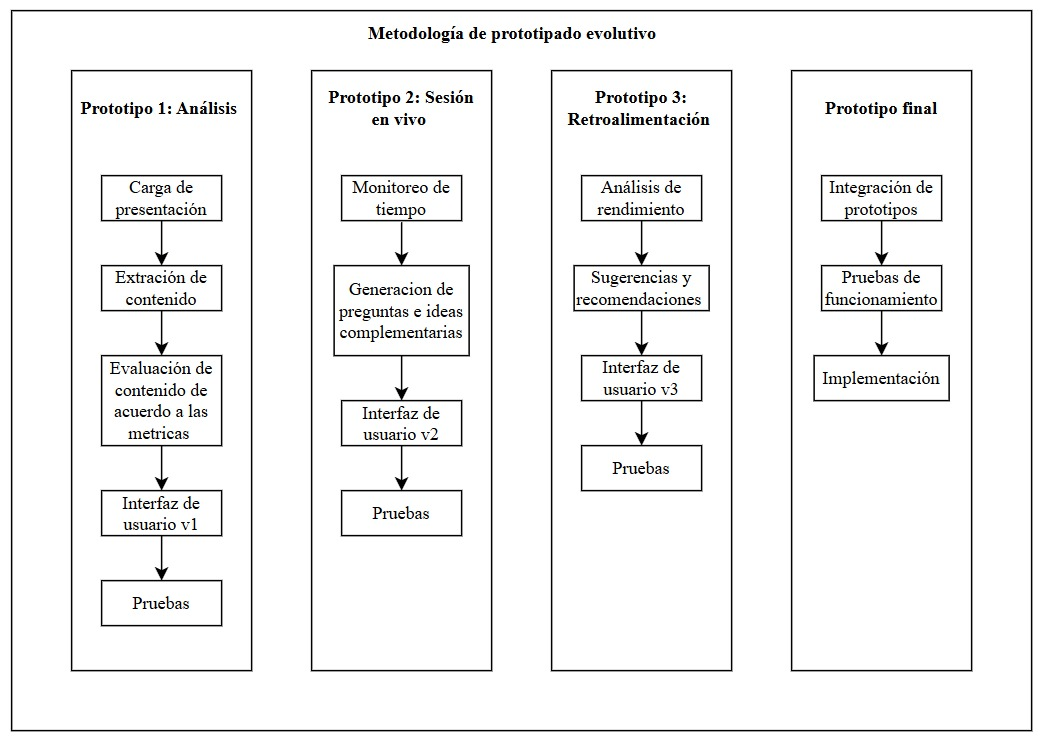
\includegraphics[width=0.9\textwidth]{TT-I/Fig01.jpeg}
    \caption{Prototipado General del Proyecto.}
    \label{fig:metodologia-prototipado-evolutivo}
\end{figure}



\clearpage
\section*{Bosquejo general}
\addcontentsline{toc}{section}{Bosquejo general}
\subsection*{Requerimientos funcionales}
\addcontentsline{toc}{subsection}{\protect\ttiiUpdatedTOC{Requerimientos funcionales}}

\renewcommand{\arraystretch}{1.0}
\setlength{\tabcolsep}{4pt}
\small

\begingroup
\ttstyle
\begin{longtable}{L{1.8cm}L{4.2cm}L{8.1cm}}
        \caption{Requerimientos funcionales}\\
        \toprule
        \textbf{ID} & \textbf{Nombre} & \textbf{Descripción} \\
        \midrule
        \endfirsthead
        \toprule
        \textbf{ID} & \textbf{Nombre} & \textbf{Descripción} \\
        \midrule
        \endhead
        \bottomrule
        \endlastfoot
        RF-01 &Selección de unidad de aprendizaje & El prototipo solicitará al usuario seleccionar la unidad de aprendizaje a la que pertenece, eligiendo entre las unidades de aprendizaje disponibles en la Escuela Superior de Cómputo. Una presentación no podrá ser cargada sin que esta selección haya sido realizada. \\
        \hairrule
        RF-01.1 & Carga de presentación & El prototipo permitirá al usuario cargar una presentación en formato .pptx. \\
        \hairrule
        RF-01.2 & Almacenamiento de presentación & El prototipo generará una copia del archivo cargado y la almacenará en un directorio dedicado a la unidad de aprendizaje que pertenezca la presentación. \\
        \hairrule
        RF-01.3 & Organización por unidad de aprendizaje & El prototipo organizará y mostrará las presentaciones agrupadas por unidad de aprendizaje, de modo que el docente pueda gestionar de forma independiente los materiales correspondientes a cada una de sus clases. \\
        \hairrule
        RF-01.4 & Visualización del temario & El prototipo permitirá al usuario consultar el temario oficial de la unidad de aprendizaje seleccionada, mostrando los temas y subtemas establecidos por la Escuela Superior de Cómputo. \\
        \hairrule
        RF-01.5 & Extracción de contenido & Durante el análisis el prototipo extraerá el número, el encabezado y el cuerpo de texto de cada diapositiva, omitiendo elementos decorativos, imágenes, animaciones y pies de página. \\
        \hairrule
        RF-01.6 & Correspondencia con el temario & Una vez extraídos los encabezados de cada diapositiva, el prototipo los comparará con los temas y subtemas del temario correspondiente a la unidad de aprendizaje seleccionada. Los temas del temario que presenten coincidencia con algún encabezado de la presentación serán marcados con un indicador visual, permitiendo al docente identificar qué temas del temario han sido abordados en sus presentaciones. \\
        \hairrule
        RF-01.7 & Eliminación de presentación & El prototipo permitirá al usuario eliminar de forma permanente una presentación previamente cargada, incluyendo todos los datos y resultados de análisis asociados a ella. \\
        \hairrule
        RF-01.8 & Eliminación por unidad de aprendizaje & El prototipo permitirá al usuario eliminar de forma permanente una unidad de aprendizaje junto con todas las presentaciones asociadas a ella y sus respectivos datos, incluyendo resultados de análisis e informes de rendimiento. Esta acción requerirá confirmación explícita del usuario antes de ejecutarse. \\
        \hairrule
        RF-01.9 & Ocultamiento de presentación & El prototipo permitirá ocultar una presentación sin eliminar el archivo ni sus datos asociados, retirándola de la vista principal y conservándola para su posterior restauración o eliminación permanente desde la vista de presentaciones ocultas. \\
        \hairrule
        RF-01.10 & Ocultamiento de unidad de aprendizaje & El prototipo permitirá ocultar una unidad de aprendizaje sin eliminarla ni eliminar sus presentaciones y datos asociados. La unidad dejará de aparecer en la vista principal y podrá restaurarse desde la vista de unidades ocultas. \\
        \hairrule
        RF-01.11 & Gestión de presentaciones ocultas & El prototipo permitirá consultar las presentaciones ocultas y, desde esa vista, restaurarlas o eliminarlas permanentemente con confirmación explícita. \\
        \hairrule
        RF-01.12 & Gestión de unidades de aprendizaje ocultas & El prototipo permitirá consultar y restaurar las unidades de aprendizaje ocultas. Desde esta vista no se ofrecerá la eliminación permanente de unidades. \\
        \hairrule
        RF-01.13 & Configuración del modelo de lenguaje & El prototipo permitirá al docente registrar su clave de API del servicio de lenguaje y seleccionar el modelo que se utilizará para el análisis y la generación de recomendaciones. La clave se almacenará de forma protegida y no se mostrará completa en la interfaz. \\
        \hairrule
        RF-02 & Análisis de presentación & El prototipo analizará la presentación indicada por el usuario, evaluando cada diapositiva con base en las métricas y parámetros predefinidos. \\
        \hairrule
        RF-02.1 & Complejidad del contenido & El prototipo calculará el Índice de Complejidad de Diapositiva (ICD) de cada diapositiva mediante la fórmula $\mathrm{ICD}=(0.6\times\mathrm{CF}+0.4\times\mathrm{DLN})\times10$. Donde CF es el complemento normalizado del índice Flesch-Szigriszt y DLN es la densidad léxica normalizada. Se determinará el porcentaje de diapositivas cuyo ICD se encuentre dentro del rango establecido de 4.0 a 6.0. Se le asignará un valor ponderado de 0.30 a esta métrica. \\
        \hairrule
        RF-02.2 & Cantidad de palabras & El prototipo contabilizará las palabras del cuerpo de cada diapositiva, excluyendo el encabezado. Las diapositivas que no superen el límite máximo de 50 palabras recibirán una puntuación de 10. Por cada 15 palabras adicionales que excedan dicho límite se descontará un punto, sin que la puntuación resultante pueda ser inferior a 0. Se le asignará un valor ponderado de 0.30 a esta métrica. \\
        \hairrule
        RF-02.3 & Estructura de la diapositiva & El prototipo evaluará la estructura interna de cada diapositiva en dos submétricas. Se le asignará un valor ponderado total de 0.25 a esta métrica. \\
        \hairrule
        RF-02.3.1 & Presencia de encabezado & El prototipo identificará si cada diapositiva cuenta con un encabezado detectable. En aquellos casos donde no se detecta un encabezado mediante la API de Gemini, se generaran recomendaciones de encabezados acordes con el contenido de la diapositiva. \\
        \hairrule
        RF-02.3.2 & Coherencia semántica encabezado-contenido & El prototipo enviará el encabezado y el cuerpo de texto de cada diapositiva a la API de Gemini, la cual asignará una calificación del 1 al 10 según el grado de relación temática entre ambos elementos. La calificación final de esta submétrica corresponderá al promedio de las puntuaciones obtenidas por las diapositivas evaluadas. \\
        \hairrule
        RF-02.4 & Hilo narrativo & El prototipo enviará el contenido de cada diapositiva junto con el de sus adyacentes a la API de Gemini, la cual asignará una calificación del 1 al 10 según el grado de coherencia y progresión temática entre diapositivas consecutivas. Se le asignará un valor ponderado de 0.15 a esta métrica. \\
        \hairrule
        RF-02.5 & Valoración global de la presentación & El prototipo calculará una valoración global de la presentación con base en los resultados de las cuatro métricas evaluadas y la clasificará en una de las siguientes categorías: Excelente, Bien, Regular o Deficiente. \\
        \hairrule
        RF-02.6 & Generación de recomendaciones & El prototipo, con apoyo de la API de Gemini, generará recomendaciones específicas para cada diapositiva que no cumpla con alguno de los criterios establecidos, preservando en todo momento los conceptos y definiciones originales del docente. \\
        \hairrule
        RF-02.7 & Actualización de la presentación & El prototipo actualizará cada diapositiva con base en las recomendaciones generadas mediante la API de Gemini. \\
        \hairrule
        RF-02.8 & Descarga de la presentación actualizada & El prototipo permitirá al docente descargar, en formato .pptx, una nueva versión de la presentación que incorpore las modificaciones realizadas con base en las recomendaciones generadas. \\
        \hairrule
        RF-02.9 & Generación de preguntas y datos de interés & El prototipo, con apoyo de la API de Gemini, generará preguntas de comprensión y datos de interés asociados al contenido de cada diapositiva, para uso opcional del docente durante la exposición. \\
        \hairrule
        RF-03 & Sesión en vivo & El prototipo habilitará un módulo de presentación en vivo que permitirá al docente exponer sus diapositivas directamente desde el prototipo. \\
        \hairrule
        RF-03.1 & Registro del tiempo estimado & Antes de iniciar la proyección, el prototipo solicitará al docente el tiempo total estimado para su exposición, expresado en minutos, el cual se utilizará como referencia en el informe de rendimiento. \\
        \hairrule
        RF-03.2 & Selección de grupo & Antes de iniciar la exposición, el prototipo permitirá al docente seleccionar el grupo correspondiente a la sesión, con el fin de asociar los tiempos registrados y facilitar su gestión y consulta por clase. \\
        \hairrule
        RF-03.2.1 & Eliminación de grupo y sus sesiones & El prototipo permitirá eliminar un grupo seleccionado asociado a una presentación. La eliminación borrará de forma permanente todas las sesiones y los tiempos registrados para ese grupo, previa confirmación explícita del docente. \\
        \hairrule
        RF-03.3 & Vista del docente & Durante la proyección, el prototipo mostrará en el equipo del docente la diapositiva activa junto con dos contadores de tiempo: uno que registra el tiempo transcurrido en la diapositiva actual y otro que acumula el tiempo global de la presentación. \\
        \hairrule
        RF-03.4 & Vista del estudiante & Durante la exposición, el prototipo mostrará en la pantalla de proyección únicamente el contenido de la diapositiva activa, sin contadores, controles ni elementos adicionales. \\
        \hairrule
        RF-03.5 & Visualización de preguntas y datos de interés & Durante la exposición, el prototipo mostrará  en la vista del docente las preguntas de comprensión y los datos de interés asociados a la diapositiva en curso. \\
        \hairrule
        RF-03.6 & Presentación estática & El prototipo ignorará las animaciones de transición y de elementos presentes en el archivo original, mostrando todas las diapositivas de forma estática. \\
        \hairrule
        RF-04 & Informe de rendimiento & Al concluir la sesión en vivo, el prototipo generará un informe de rendimiento donde mostrará un análisis de los datos de tiempo registrados durante la exposición. \\
        \hairrule
        RF-04.1 & Comparativa de tiempos & El informe de rendimiento presentará una comparativa entre el tiempo total registrado por el prototipo, el tiempo estimado por el docente al inicio de la sesión y el tiempo recomendado por la IA con base en el contenido analizado. \\
        \hairrule
        RF-04.2 & Identificación de desviaciones por diapositiva & El informe identificará las diapositivas con mayor y menor desviación respecto a cualquiera de los tiempos de referencia. \\
        \hairrule
        RF-05 & Historial y gestión de versiones & El usuario podrá consultar el historial de versiones de cada presentación. Para cada versión, el prototipo mostrará la evaluación y las métricas desglosadas por diapositiva, así como las recomendaciones de IA asociadas a cada diapositiva. El docente podrá descargar en formato .pptx cada versión que incorpore los cambios sugeridos por la IA, sin sobrescribir el archivo original ni otras versiones. \\
\end{longtable}
\endgroup
\normalsize
\renewcommand{\arraystretch}{1}

\clearpage
\subsection*{Arquitectura general del prototipo}
\addcontentsline{toc}{subsection}{Arquitectura general del prototipo}

\subsubsection*{Arquitectura en Capas}
\addcontentsline{toc}{subsubsection}{Arquitectura en Capas}
Con el fin de estructurar el prototipo de forma modular, escalable y alineada a la metodología de prototipado evolutivo, el proyecto se basa en una arquitectura en capas. Esta permite organizar de manera jerárquica los componentes, asignando responsabilidades desde el nivel más alto hasta el más bajo, lo que facilita la integración de nuevas funcionalidades y permite una mejor gestión de estas sin afectar las ya establecidas.

\begin{figure}[!htbp]
    \centering
    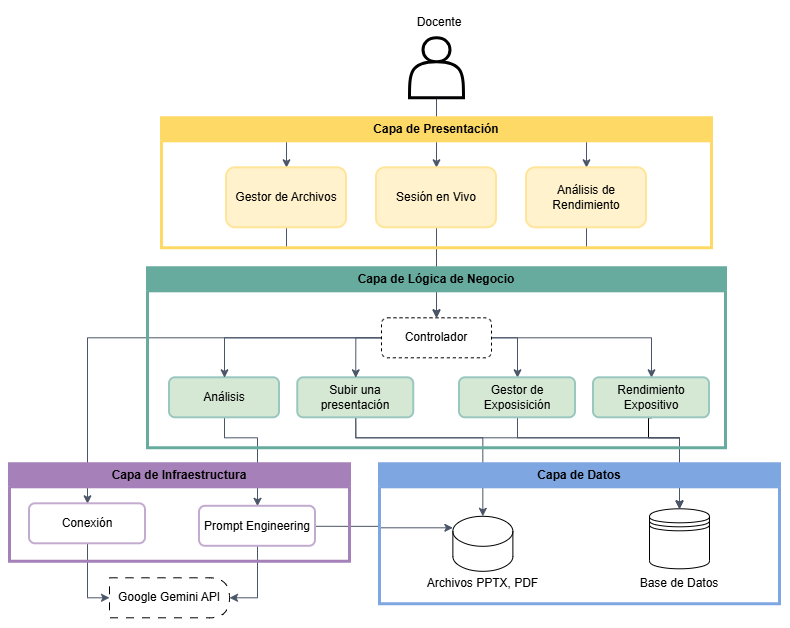
\includegraphics[width=0.78\textwidth]{TT-I/Fig02.png}
    \caption{Arquitectura General del Prototipo.}
    \label{fig:arquitectura-general-prototipo}
\end{figure}
\FloatBarrier

El prototipo se organiza mediante cuatro capas principales:
\begingroup
\small
\RaggedRight
\begin{enumerate}
    \item \textbf{Capa de presentación:} Agrupa los componentes de la interfaz gráfica implementados en el módulo \texttt{app/presentation}. Aquí se incluyen las vistas principales (carga, análisis y navegación), así como los widgets que componen cada interfaz.
    \item \textbf{Capa de lógica de negocio:} Implementada en los módulos \texttt{app/core/controller} y \texttt{app/core/logic}, actúa como intermediaria entre la interfaz y la lógica del programa. Esta coordina el flujo de datos entre ambas sin mezclar responsabilidades. Además, concentra el núcleo funcional: los algoritmos de cálculo de métricas (complejidad lingüística, conteo de palabras, densidad léxica, hilo narrativo y estructura del encabezado).
    \item \textbf{Capa de infraestructura:} Implementada en el módulo \texttt{app/infrastructure/ai}, gestiona la comunicación del prototipo con servicios externos. Encapsula en \texttt{llm\_provider.py} el cliente de conexión hacia la API de Google Gemini, administrando la autenticación, el envío de solicitudes y el manejo de errores de comunicación de forma aislada del resto del prototipo. Centraliza en \texttt{prompts.py} los prompts diseñados mediante ingeniería de prompts para cada tarea delegada al modelo, garantizando que las instrucciones enviadas sean consistentes y modificables de forma independiente sin afectar la lógica de negocio ni los componentes de métricas.
    \item \textbf{Capa de datos:} Definida en \texttt{app/data}, gestiona la persistencia mediante una base de datos SQLite, el repositorio de presentaciones y las consultas de almacenamiento local.
\end{enumerate}
\endgroup

La elección de esta arquitectura sobre otras alternativas se debe a que, en primer lugar, este modelo permite la testabilidad independiente por capa; dado que cada funcionalidad reside de forma aislada, es posible verificar el comportamiento de cada algoritmo sin necesidad de invocar la interfaz gráfica. En segundo lugar, permite sustituir o actualizar el servicio o modelo de IA sin tener que modificar toda la lógica del prototipo. Por último, la arquitectura por capas favorece la independencia de desarrollo; la separación de responsabilidades permite que los integrantes del equipo trabajen de forma simultánea en componentes distintos sin generar conflictos entre módulos.

\subsubsection*{Diagrama de bases de datos}
\addcontentsline{toc}{subsubsection}{Diagrama de bases de datos}

El diseño de la base de datos del prototipo refleja la estructura funcional del prototipo y las relaciones entre sus componentes principales. El modelo relacional se organiza en torno a dos ejes: el catálogo institucional, que almacena la información estática de las unidades de aprendizaje, sus unidades temáticas, temas y subtemas correspondientes a los planes de estudio de la Escuela Superior de Cómputo; y el eje operativo, que gestiona las presentaciones cargadas por los docentes, su historial de versiones y los resultados del análisis generado por el prototipo.

La Figura 3 presenta el modelo relacional de la base de datos.

\begin{figure}[!htbp]
    \centering
    \includegraphics[width=0.9\textwidth]{TT-I/Fig03.png}
    \caption{Modelo Relacional de la Base de Datos.}
    \label{fig:modelo-relacional-base-datos}
\end{figure}


\clearpage
\section*{Prototipos}
\addcontentsline{toc}{section}{Prototipos}
\subsection*{Prototipo 1: Análisis de presentaciones}
\addcontentsline{toc}{subsection}{Prototipo 1: Análisis de presentaciones}

\textbf{Introducción}

El prototipo 1 constituye la base funcional del proyecto, ya que implementa el núcleo analítico sobre el cual se construyen los prototipos posteriores. Su desarrollo abarca desde la gestión de unidades de aprendizaje y la carga de presentaciones hasta la evaluación automática del contenido de cada diapositiva y la generación de recomendaciones personalizadas mediante la API de Google Gemini. Este prototipo representa la primera versión funcional entregable del proyecto y establece la arquitectura de cuatro capas, la estructura de la base de datos y los algoritmos de cálculo de métricas que serán reutilizados y extendidos en las iteraciones siguientes.

\textbf{Objetivo}

Implementar un prototipo funcional que permita al docente cargar una presentación en formato .pptx, organizarla por unidad de aprendizaje y obtener una evaluación automática de su contenido con base en las cuatro métricas definidas: complejidad del contenido, cantidad de palabras por diapositiva, estructura de la diapositiva e hilo narrativo. A partir de los resultados del análisis, el prototipo generará recomendaciones específicas por diapositiva mediante la integración con la API de Google Gemini, preservando en todo momento los conceptos originales del docente. Adicionalmente, el prototipo permitirá visualizar la cobertura temática de la presentación respecto al temario oficial de la unidad de aprendizaje y consultar el historial de versiones de cada presentación para comparar la evolución de sus resultados a lo largo del tiempo.

\subsubsection*{Especificaciones (Historias de Usuario) del Prototipo 1}
\addcontentsline{toc}{subsubsection}{Especificaciones (Historias de Usuario) del Prototipo 1}

\begin{table}[H]
    \centering
    \renewcommand{\arraystretch}{1.2}
    \ttstyle
    \begin{tabular}{p{2.5cm}p{11cm}}
        \toprule
        \textbf{ID} & \textbf{Historia de Usuario --- Seleccionar Unidad de Aprendizaje} \\
        \midrule
        HU-01 & Como docente, quiero seleccionar la unidad de aprendizaje a la que pertenece mi presentación antes de cargarla, para mantener mis materiales organizados por clase. \\
        \hairrule
        \textbf{Prioridad} & \textbf{Criterios de aceptación} \\
        \hairrule
        Alta & El prototipo mostrará el listado de unidades de aprendizaje disponibles en la Escuela Superior de Cómputo. La selección de una unidad de aprendizaje es obligatoria; el prototipo no permitirá continuar con la carga sin que esta haya sido realizada. 
        
        El prototipo mostrará el nombre completo de la unidad de aprendizaje seleccionada como confirmación antes de continuar. \\
        \bottomrule
    \end{tabular}
    \caption{Historia de Usuario — Seleccionar Unidad de Aprendizaje}
    \label{tab:hu-seleccionar-unidad}
\end{table}


\begin{table}[H]
    \centering
    \renewcommand{\arraystretch}{1.2}
    \ttstyle
    \begin{tabular}{p{2.5cm}p{11cm}}
        \toprule
        \textbf{ID} & \textbf{Historia de Usuario --- Cargar Presentación} \\
        \midrule
        HU-02 & Como docente, quiero cargar una presentación en el prototipo, para poder analizar su contenido y recibir retroalimentación. \\
        \hairrule
        \textbf{Prioridad} & \textbf{Criterios de aceptación} \\
        \hairrule
        Alta & El prototipo únicamente permitirá seleccionar archivos con extensión .pptx. 
        
        El prototipo validará que el archivo no exceda el tamaño máximo permitido de 30 MB. 
        
        El prototipo validará que no exista en la unidad de aprendizaje seleccionada una presentación con el mismo nombre.
        
        El prototipo extraerá el encabezado y el cuerpo de texto de cada diapositiva, omitiendo imágenes, animaciones, elementos decorativos y pies de página.
        
        El prototipo generará una copia del archivo en el directorio de almacenamiento, organizado dentro de una carpeta correspondiente a la unidad de aprendizaje y una subcarpeta con el nombre de la presentación. 
        
        Al concluir la carga exitosamente, el prototipo mostrará un mensaje de confirmación e incluirá en la interfaz el nombre de la presentación y la vista preliminar de su primera diapositiva. \\
        \bottomrule
    \end{tabular}
    \caption{Historia de Usuario — Cargar Presentación}
    \label{tab:hu-cargar-presentacion}
\end{table}


\begin{table}[H]
    \centering
    \renewcommand{\arraystretch}{1.2}
    \ttstyle
    \begin{tabular}{p{2.5cm}p{11cm}}
        \toprule
        \textbf{ID} & \textbf{Historia de Usuario --- Cargar Nueva Versión} \\
        \midrule
        HU-03 & Como docente, quiero cargar una versión actualizada de una presentación previamente registrada, para comparar los resultados del análisis y verificar las mejoras realizadas. \\
        \hairrule
        \textbf{Prioridad} & \textbf{Criterios de aceptación} \\
        \hairrule
        Alta & El prototipo mostrará una advertencia de confirmación antes de registrar la nueva versión. 
        
        El prototipo creará una nueva entrada de versión sin eliminar ni reemplazar las versiones anteriores, conservando su historial de análisis. 
        
        La interfaz mostrará la versión más reciente como versión activa de la presentación. \\
        \bottomrule
    \end{tabular}
    \caption{ Historia de Usuario — Cargar Nueva Versión}
    \label{tab:hu-cargar-nueva-version}
\end{table}


\begin{table}[H]
    \centering
    \renewcommand{\arraystretch}{1.2}
    \ttstyle
    \begin{tabular}{p{2.5cm}p{11cm}}
        \toprule
        \textbf{ID} & \textbf{Historia de Usuario --- Consultar Temario y Cobertura} \\
        \midrule
        HU-04 & Como docente, quiero visualizar el temario de la unidad de aprendizaje y saber qué temas de ese temario cubre mi presentación, para identificar si existen temas pendientes de abordar. \\
        \hairrule
        \textbf{Prioridad} & \textbf{Criterios de aceptación} \\
        \hairrule
        Media & El prototipo mostrará el temario oficial de la unidad de aprendizaje seleccionada, con sus temas y subtemas. 
        
        El prototipo comparará los encabezados extraídos de la presentación con los temas y subtemas del temario. Los temas del temario que presenten correspondencia con algún encabezado de la presentación serán marcados con un indicador visual diferenciado. Los temas sin correspondencia permanecerán sin marcador, permitiendo al docente identificar los contenidos no cubiertos. \\
        \bottomrule
    \end{tabular}
    \caption{Historia de Usuario — Consultar Temario y Cobertura}
    \label{tab:hu-consultar-temario-cobertura}
\end{table}

\begin{table}[H]
    \centering
    \renewcommand{\arraystretch}{1.2}
    \ttstyle
    \begin{tabular}{p{2.5cm}p{11cm}}
        \toprule
        \textbf{ID} & \textbf{Historia de Usuario — Analizar Presentación} \\
        \midrule
        HU-05 & Como docente, quiero que el prototipo analice mi presentación con base en las métricas definidas, para identificar áreas de mejora en el contenido y la estructura de mis diapositivas. \\
        \hairrule
        \textbf{Prioridad} & \textbf{Criterios de aceptación} \\
        \hairrule
        Alta & Antes de iniciar el análisis, el prototipo verificará que exista conectividad a internet y que se haya configurado una clave de API y un modelo de lenguaje disponibles.
        
        El prototipo aplicará las cuatro métricas definidas —complejidad del contenido, cantidad de palabras, estructura de la diapositiva e hilo narrativo— al texto extraído de cada diapositiva. 
        
        El prototipo mostrará una barra de progreso durante la ejecución del análisis. Al finalizar el análisis, el prototipo mostrará un mensaje de confirmación de conclusión. 
        
        El prototipo mostrará los resultados del análisis desglosados por diapositiva, incluyendo la puntuación obtenida en cada métrica. \\
        \bottomrule
    \end{tabular}
    \caption{Historia de Usuario — Analizar Presentación}
    \label{tab:hu-analizar-presentacion}
\end{table}

\begin{table}[H]
    \centering
    \renewcommand{\arraystretch}{1.2}
    \ttstyle
    \begin{tabular}{p{2.5cm}p{11cm}}
        \toprule
        \textbf{ID} & \textbf{Historia de Usuario --- Consultar y aplicar recomendaciones} \\
        \midrule
        HU-06 & Como docente, quiero consultar las recomendaciones generadas para cada diapositiva y aplicarlas automáticamente, para obtener una nueva versión de mi presentación con las mejoras sugeridas. \\
        \hairrule
        \textbf{Prioridad} & \textbf{Criterios de aceptación} \\
        \hairrule
        Alta & El prototipo mostrará las recomendaciones generadas por la API de Gemini para cada diapositiva que no haya cumplido con alguno de los criterios de las métricas evaluadas. Las recomendaciones se mostrarán asociadas a la diapositiva correspondiente e indicarán la métrica específica que originó cada observación. 
        
        El prototipo permitirá aplicar automáticamente las recomendaciones generadas y realizará las modificaciones correspondientes en cada diapositiva.

        Al concluir el proceso, el prototipo generará una nueva versión de la presentación con los cambios aplicados, sin modificar el archivo original, y permitirá descargar esa versión en formato .pptx.
        
        Las diapositivas que hayan cumplido con todos los criterios no mostrarán recomendaciones pendientes ni requerirán modificaciones. \\
        \bottomrule
    \end{tabular}
    \caption{Historia de Usuario — Consultar y aplicar recomendaciones}
    \label{tab:hu-consultar-recomendaciones}
\end{table}


\begin{table}[H]
    \centering
    \renewcommand{\arraystretch}{1.2}
    \ttstyle
    \begin{tabular}{p{2.5cm}p{11cm}}
        \toprule
        \textbf{ID} & \textbf{Historia de Usuario --- Consultar Historial de Versiones} \\
        \midrule
        HU-07 & Como docente, quiero consultar el historial de versiones de una presentación, incluidas aquellas que contienen los cambios aplicados a partir de las recomendaciones, para revisar la evolución de mi material a lo largo del tiempo. \\
        \hairrule
        \textbf{Prioridad} & \textbf{Criterios de aceptación} \\
        \hairrule
        Media & El prototipo verificará que exista al menos una versión de la presentación antes de mostrar el historial.
        
        El prototipo mostrará, en orden cronológico, todas las versiones de la presentación seleccionada, incluida la versión original y las versiones generadas con cambios sugeridos por la IA.
        
        Por cada versión analizada, el prototipo permitirá consultar la evaluación y las recomendaciones asociadas a cada diapositiva, además de mostrar la fecha de creación, la valoración global y las modificaciones aplicadas. Para cada versión con cambios sugeridos, permitirá descargar el archivo .pptx correspondiente sin alterar otras versiones. \\
        \bottomrule
    \end{tabular}
    \caption{Historia de Usuario — Consultar Historial de Versiones}
    \label{tab:hu-historial-versiones}
\end{table}

\begin{table}[H]
    \centering
    \renewcommand{\arraystretch}{1.2}
    \ttstyle
    \begin{tabular}{p{2.5cm}p{11cm}}
        \toprule
        \textbf{ID} & \textbf{Historia de Usuario --- Eliminar Presentación} \\
        \midrule
        HU-08 & Como docente, quiero eliminar presentaciones que ya no necesito, para mantener organizado el repositorio y evitar almacenar información innecesaria. \\
        \hairrule
        \textbf{Prioridad} & \textbf{Criterios de aceptación} \\
        \hairrule
        Baja & El prototipo mostrará una advertencia de confirmación explícita antes de ejecutar la eliminación. 
        
        El prototipo realizará la eliminación en cascada, asegurando que se eliminen el archivo, todas sus versiones y todos los datos y resultados de análisis asociados. La interfaz se actualizará automáticamente para reflejar los cambios. \\
        \bottomrule
    \end{tabular}
    \caption{Historia de Usuario — Eliminar Presentación}
    \label{tab:hu-eliminar-presentacion}
\end{table}




\begin{table}[H]
    \centering
    \renewcommand{\arraystretch}{1.2}
    \ttstyle
    \begin{tabular}{p{2.5cm}p{11cm}}
        \toprule
        \textbf{ID} & \textbf{Historia de Usuario --- Eliminar Unidad de Aprendizaje} \\
        \midrule
        HU-09 & Como docente, quiero eliminar una unidad de aprendizaje junto con todas sus presentaciones, para depurar de forma completa los materiales de una clase que ya no imparto. \\
        \hairrule
        \textbf{Prioridad} & \textbf{Criterios de aceptación} \\
        \hairrule
        Baja & El prototipo mostrará una advertencia de confirmación explícita que indique que la acción eliminará la unidad de aprendizaje y todas las presentaciones, versiones y datos asociados a ella. 
        
        El prototipo ejecutará la eliminación en cascada únicamente tras recibir la confirmación explícita del usuario. La interfaz se actualizará automáticamente para reflejar que la unidad de aprendizaje ya no está disponible. \\
        \bottomrule
    \end{tabular}
    \caption{Historia de Usuario — Eliminar Unidad de Aprendizaje}
    \label{tab:hu-eliminar-unidad-aprendizaje}
\end{table}

\begin{table}[H]
    \centering
    \renewcommand{\arraystretch}{1.2}
    \ttstyle
    \begin{tabular}{p{2.5cm}p{11cm}}
        \toprule
        \textbf{ID} & \textbf{Historia de Usuario --- Ocultar presentación} \\
        \midrule
        HU-10 & Como docente, quiero ocultar una presentación que no deseo ver en la lista principal, para conservarla junto con su análisis y poder recuperarla posteriormente. \\
        \hairrule
        \textbf{Prioridad} & \textbf{Criterios de aceptación} \\
        \hairrule
        Media & Al ocultar una presentación, el prototipo la retirará de la lista principal sin eliminar su archivo, versiones, análisis, recomendaciones ni sesiones registradas. La presentación estará disponible en la vista de elementos ocultos. \\
        \bottomrule
    \end{tabular}
    \caption{Historia de Usuario --- Ocultar presentación}
    \label{tab:hu-ocultar-presentacion}
\end{table}

\begin{table}[H]
    \centering
    \renewcommand{\arraystretch}{1.2}
    \ttstyle
    \begin{tabular}{p{2.5cm}p{11cm}}
        \toprule
        \textbf{ID} & \textbf{Historia de Usuario --- Gestionar presentaciones ocultas} \\
        \midrule
        HU-11 & Como docente, quiero consultar las presentaciones ocultas y poder restaurarlas o eliminarlas permanentemente, para decidir si deseo recuperarlas o depurarlas definitivamente. \\
        \hairrule
        \textbf{Prioridad} & \textbf{Criterios de aceptación} \\
        \hairrule
        Media & La vista mostrará las presentaciones ocultas. La opción de restaurar devolverá la presentación a su unidad de aprendizaje y lista principal sin perder sus datos. La opción de eliminación permanente solicitará confirmación e incluirá los datos y versiones asociados. \\
        \bottomrule
    \end{tabular}
    \caption{Historia de Usuario --- Gestionar presentaciones ocultas}
    \label{tab:hu-gestionar-presentaciones-ocultas}
\end{table}

\begin{table}[H]
    \centering
    \renewcommand{\arraystretch}{1.2}
    \ttstyle
    \begin{tabular}{p{2.5cm}p{11cm}}
        \toprule
        \textbf{ID} & \textbf{Historia de Usuario --- Ocultar unidad de aprendizaje} \\
        \midrule
        HU-12 & Como docente, quiero ocultar una unidad de aprendizaje que no utilizo actualmente, para retirarla de la vista principal sin perder sus presentaciones ni registros. \\
        \hairrule
        \textbf{Prioridad} & \textbf{Criterios de aceptación} \\
        \hairrule
        Media & Al ocultar la unidad, el prototipo la retirará de la lista principal y conservará sus presentaciones, versiones, análisis y sesiones. La unidad podrá encontrarse en la vista de unidades ocultas. \\
        \bottomrule
    \end{tabular}
    \caption{Historia de Usuario --- Ocultar unidad de aprendizaje}
    \label{tab:hu-ocultar-unidad}
\end{table}

\begin{table}[H]
    \centering
    \renewcommand{\arraystretch}{1.2}
    \ttstyle
    \begin{tabular}{p{2.5cm}p{11cm}}
        \toprule
        \textbf{ID} & \textbf{Historia de Usuario --- Restaurar unidades de aprendizaje ocultas} \\
        \midrule
        HU-13 & Como docente, quiero consultar y restaurar unidades de aprendizaje ocultas, para volver a mostrarlas en la lista principal cuando las necesite. \\
        \hairrule
        \textbf{Prioridad} & \textbf{Criterios de aceptación} \\
        \hairrule
        Media & La vista de unidades ocultas mostrará las unidades disponibles y ofrecerá únicamente la acción de restaurar. Al restaurar una unidad, esta reaparecerá en la lista principal junto con sus datos y presentaciones asociados. No se ofrecerá la eliminación permanente desde esta vista. \\
        \bottomrule
    \end{tabular}
    \caption{Historia de Usuario --- Restaurar unidades de aprendizaje ocultas}
    \label{tab:hu-restaurar-unidades-ocultas}
\end{table}

\begin{table}[H]
    \centering
    \renewcommand{\arraystretch}{1.2}
    \ttstyle
    \begin{tabular}{p{2.5cm}p{11cm}}
        \toprule
        \textbf{ID} & \textbf{Historia de Usuario --- Configurar servicio de IA} \\
        \midrule
        HU-14 & Como docente, quiero ingresar mi clave de API y elegir el modelo de lenguaje, para configurar el servicio de IA que analizará mis presentaciones. \\
        \hairrule
        \textbf{Prioridad} & \textbf{Criterios de aceptación} \\
        \hairrule
        Alta & El prototipo ofrecerá una sección de configuración con campos para la clave de API y la selección de un modelo disponible. Permitirá guardar y validar la configuración; ocultará la clave después de guardarla y mostrará un mensaje claro si falta o no es válida, sin iniciar el análisis. \\
        \bottomrule
    \end{tabular}
    \caption{Historia de Usuario --- Configurar servicio de IA}
    \label{tab:hu-configurar-servicio-ia}
\end{table}

\subsubsection*{Arquitectura del Prototipo 1}
\addcontentsline{toc}{subsubsection}{Arquitectura del Prototipo 1}

El prototipo 1 adopta una arquitectura de cuatro capas que separa las responsabilidades del prototipo en niveles independientes, facilitando el mantenimiento de cada componente y la incorporación de nuevas funcionalidades en iteraciones posteriores del desarrollo.

La capa de presentación constituye el punto de interacción entre el docente y el prototipo. A través de ella, el usuario gestiona la carga de archivos y consulta los resultados del análisis generado. La capa de lógica de negocio concentra el procesamiento central del prototipo: un controlador coordina las operaciones entre el extractor de texto, responsable de obtener el contenido textual de cada diapositiva a partir del archivo .pptx, el motor de métricas, que ejecuta el cálculo de los cuatro indicadores definidos, y el módulo de sugerencias de optimización, que formula las recomendaciones dirigidas al docente. La capa de infraestructura gestiona la comunicación con servicios externos: encapsula el cliente de conexión hacia la API de Google Gemini y centraliza los prompts diseñados mediante ingeniería de prompts, garantizando que las instrucciones enviadas al modelo estén estructuradas de forma consistente e independiente del resto de la lógica de negocio. La capa de datos gestiona la persistencia del prototipo, almacenando tanto los archivos de presentación como los resultados del análisis en la base de datos mediante una instancia SQLite administrada localmente.

La Figura 4 presenta el diagrama de la arquitectura descrita.
\begin{figure}[!htbp]
    \centering
    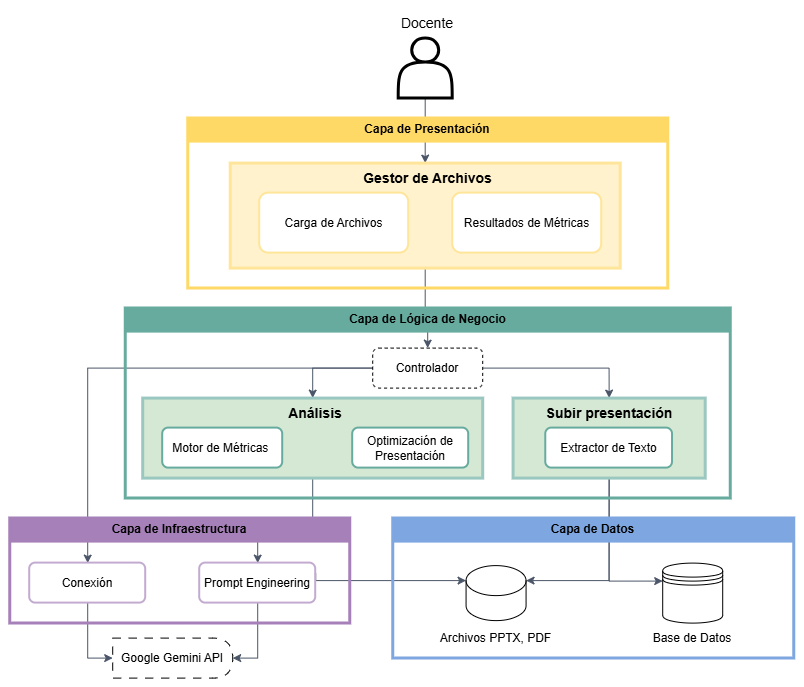
\includegraphics[width=0.85\textwidth]{TT-I/Fig04.png}
    \caption{Arquitectura del Prototipo 1.}
    \label{fig:arquitectura-prototipo-1}
\end{figure}
\FloatBarrier

\subsubsection*{Diagrama de componentes del Prototipo 1}
\addcontentsline{toc}{subsubsection}{Diagrama de componentes del Prototipo 1}
El diagrama de componentes detalla la organización interna del prototipo 1 a nivel de módulos de software, mostrando cómo se distribuyen las responsabilidades del prototipo entre los distintos archivos que lo conforman y las relaciones de uso entre ellos. A diferencia del diagrama de arquitectura, que describe las capas del prototipo de forma conceptual, el diagrama de componentes refleja la estructura real de implementación.

La capa de presentación se divide en dos módulos. El primero, Subject \& Content Management, agrupa los componentes visuales encargados de la gestión de unidades de aprendizaje y la carga de presentaciones: un panel de contenido, una barra lateral, una barra superior y un panel derecho, todos coordinados por \texttt{main\_gui.py}. El segundo, Evaluation View, concentra los componentes de visualización del análisis: el panel de presentación y el panel de resultados, coordinados por \texttt{analysis\_gui.py}. Ambos módulos se comunican con el resto del prototipo a través de \texttt{navigator.py}, que gestiona la navegación entre vistas.

La capa de lógica de negocio se organiza en tres agrupaciones. El módulo Controller contiene los controladores de unidades de aprendizaje, presentaciones y análisis, que actúan como intermediarios entre la interfaz y la lógica interna. El módulo Logic alberga los componentes de validación e integridad de archivos —generación de hash y validación de formato— junto con los componentes de procesamiento y análisis, responsables de la extracción de texto, la clasificación de diapositivas, el conteo de elementos y el cálculo de la puntuación global de la presentación. El módulo Metrics concentra los cinco componentes de cálculo de métricas: \texttt{icd.py} para la complejidad del contenido, \texttt{word\_count.py} para la cantidad de palabras, \texttt{readability.py} para la legibilidad, \texttt{narrative\_thread.py} para el hilo narrativo y \texttt{header\_structure.py} para la estructura de la diapositiva.

La capa de infraestructura se implementa en el módulo \texttt{app/infrastructure/ai} y agrupa dos componentes. El primero, \texttt{llm\_provider.py}, encapsula la conexión con la API de Google Gemini, gestionando la autenticación, el envío de solicitudes y el manejo de errores de comunicación de forma aislada del resto del prototipo. El segundo, \texttt{prompts.py}, centraliza los prompts diseñados mediante ingeniería de prompts para cada tarea delegada al modelo: evaluación de coherencia semántica, análisis de hilo narrativo, generación de recomendaciones y producción de preguntas y datos de interés. Esta separación garantiza que cualquier modificación en las instrucciones enviadas al modelo o en el proveedor del servicio pueda realizarse sin afectar la lógica de negocio ni los componentes de métricas.

La capa de datos gestiona la persistencia mediante \texttt{persistence.py} y \texttt{queries.py}, coordinados por \texttt{database\_manager.py}, que administra todas las operaciones sobre la base de datos \texttt{ai\_analyzer.db}.

La Figura 5 presenta el diagrama de componentes descrito.

\begin{figure}[!htbp]
    \centering
    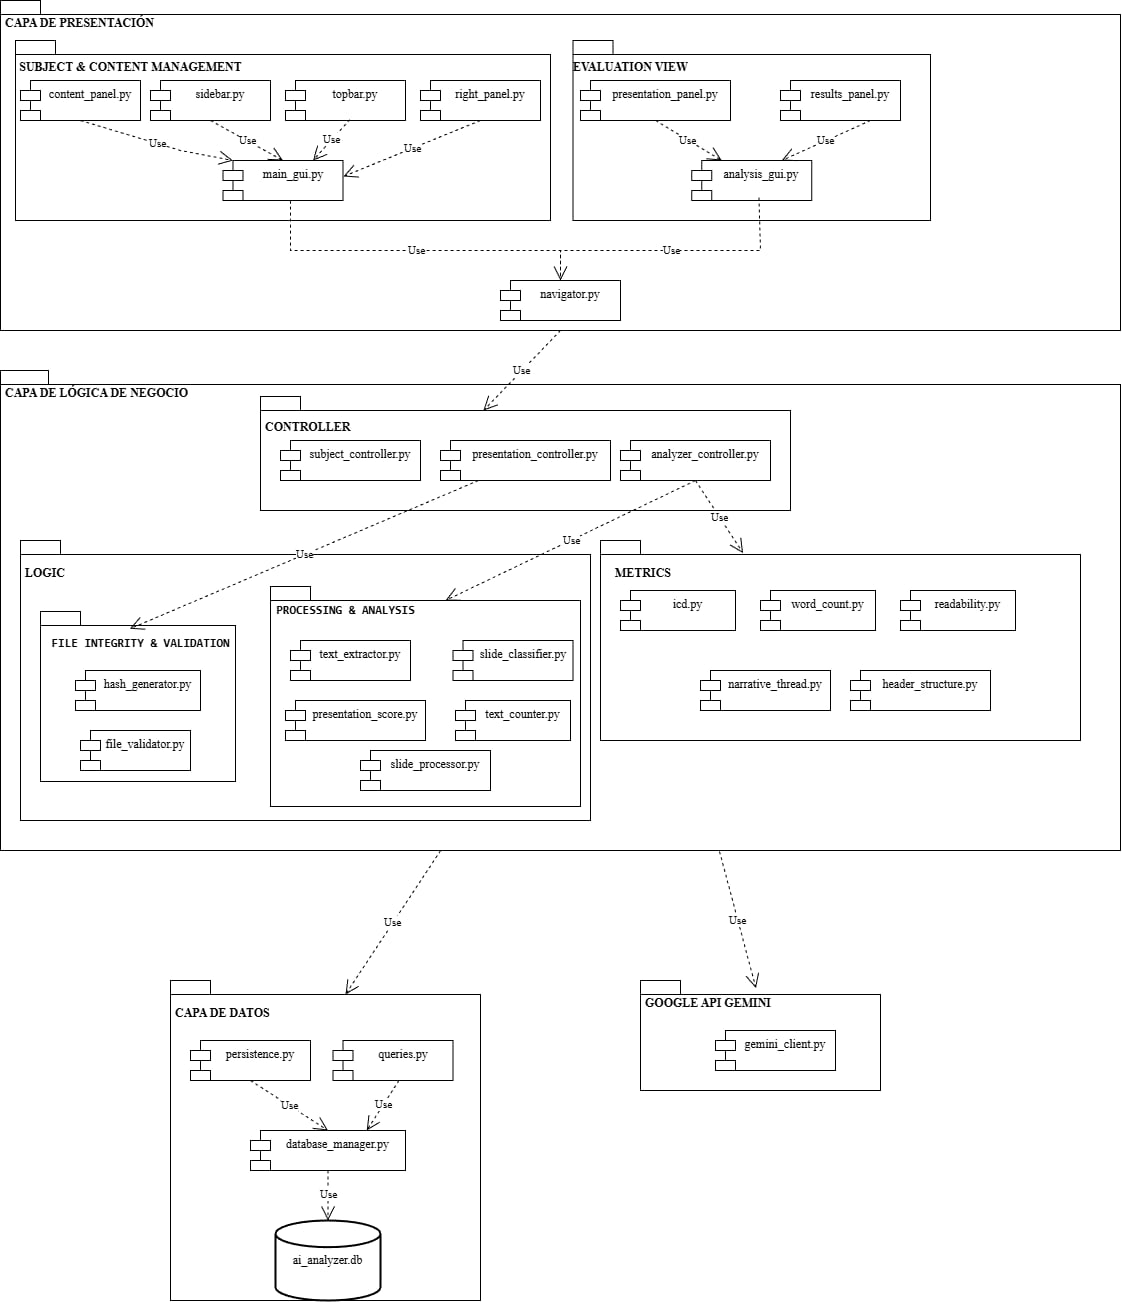
\includegraphics[width=0.9\textwidth]{TT-I/Fig05.jpg}
    \caption{Diagrama de Componentes del Prototipo 1.}
    \label{fig:componentes-prototipo-1}
\end{figure}
\clearpage




\subsubsection*{Diseño de la interfaz del Prototipo 1}
\addcontentsline{toc}{subsubsection}{Diseño de la interfaz del Prototipo 1}

Los mockups se organizan como una secuencia de interacción que cubre la configuración del servicio de IA, la gestión de unidades de aprendizaje y presentaciones, y el análisis con sus recomendaciones e historial de versiones. Esta selección se vincula con las historias de usuario HU-01 a HU-14.

\newcommand{\mockupPuno}[2]{%
  \begin{figure}[!htbp]
    \centering
    \includegraphics[width=0.8\textwidth]{TT-I/Mockup-P1-#1.png}
    \caption{#2}
    \label{fig:mockup-p1-#1}
  \end{figure}%
}

\mockupPuno{01}{Pantalla principal y acceso a la configuración de la clave de API y el modelo de lenguaje.}
\mockupPuno{02}{Formulario para ingresar la clave de API y seleccionar el modelo de lenguaje.}
\mockupPuno{03}{Acceso a la opción para agregar o seleccionar una unidad de aprendizaje.}
\mockupPuno{04}{Catálogo de unidades de aprendizaje disponibles para seleccionar.}
\mockupPuno{05}{Acceso al temario de la unidad de aprendizaje seleccionada.}
\mockupPuno{06}{Temario de la unidad de aprendizaje y cobertura temática identificada en la presentación.}
\mockupPuno{07}{Acceso a la opción para cargar una nueva presentación.}
\mockupPuno{08}{Explorador de archivos para seleccionar una presentación en formato .pptx.}
\mockupPuno{09}{Confirmación de que la presentación se cargó correctamente.}
\mockupPuno{10}{Mensaje de error al intentar cargar un archivo cuya extensión no es .pptx.}
\mockupPuno{11}{Mensaje de error al intentar cargar un archivo que supera el límite de 30 MB.}
\mockupPuno{12}{Selección de una presentación existente para cargar una nueva versión.}
\mockupPuno{13}{Explorador de archivos para seleccionar el archivo de la nueva versión.}
\mockupPuno{14}{Solicitud de confirmación antes de registrar la nueva versión y conservar las anteriores.}
\mockupPuno{15}{Confirmación de que la nueva versión se registró correctamente y quedó activa.}
\mockupPuno{16}{Menú de opciones de una presentación cargada.}
\mockupPuno{17}{Selección de la opción para ocultar una presentación.}
\mockupPuno{18}{Acceso a la lista de presentaciones ocultas.}
\mockupPuno{19}{Modal de presentaciones ocultas con las opciones para restaurar o eliminar una presentación y confirmación de su restauración.}
\mockupPuno{20}{Selección de la opción para eliminar una presentación desde su menú principal.}
\mockupPuno{21}{Mensaje de confirmación antes de eliminar una presentación.}
\mockupPuno{22}{Acceso a la opción para eliminar una unidad de aprendizaje.}
\mockupPuno{23}{Opciones para ocultar o eliminar la unidad de aprendizaje, o cancelar la acción; selección de ocultar.}
\mockupPuno{24}{Acceso a la lista de unidades de aprendizaje ocultas.}
\mockupPuno{25}{Lista de unidades de aprendizaje ocultas y opción para restaurar una unidad.}
\mockupPuno{26}{Nuevo acceso a la opción para eliminar una unidad de aprendizaje.}
\mockupPuno{27}{Opciones para ocultar o eliminar la unidad de aprendizaje, o cancelar la acción; selección de eliminar.}
\mockupPuno{28}{Vista principal después de eliminar la unidad de aprendizaje seleccionada.}
\mockupPuno{29}{Selección de la opción para analizar una presentación.}
\mockupPuno{30}{Mensaje de error cuando no hay conexión a internet para realizar el análisis.}
\mockupPuno{31}{Indicador de progreso durante el análisis de la presentación.}
\mockupPuno{32}{Resultados del análisis con la evaluación y las recomendaciones por diapositiva.}
\mockupPuno{33}{Acción para aplicar los cambios sugeridos y generar una nueva versión de la presentación.}
\mockupPuno{34}{Regreso a la vista principal después de consultar el análisis.}
\mockupPuno{35}{Opciones adicionales disponibles después de analizar la presentación.}
\mockupPuno{36}{Comparación entre una presentación analizada y otra que aún no cuenta con análisis.}
\mockupPuno{37}{Selección de la opción para consultar el historial de versiones desde el menú de la presentación.}
\mockupPuno{38}{Historial con las versiones registradas de la presentación.}

\let\mockupPuno\relax

\clearpage
\subsubsection*{Desarrollo del Prototipo 1}
\addcontentsline{toc}{subsubsection}{Desarrollo del Prototipo 1}

La fase de desarrollo del prototipo 1 comprende la implementación de los módulos definidos en la arquitectura de cuatro capas descrita en la sección anterior, abarcando desde la gestión de unidades de aprendizaje y la carga de presentaciones hasta el cálculo de métricas, la integración con la API de Google Gemini y la visualización de resultados.

Con el propósito de documentar el comportamiento del prototipo 1 y la interacción entre sus componentes, se presentan los diagramas de secuencia de sus principales flujos. Estos se organizan en el orden de uso: configuración del servicio de IA; consulta y gestión de unidades de aprendizaje; carga, actualización y administración de presentaciones; análisis y aplicación de cambios; y consulta de cobertura temática e historial.

Se incluyen diagramas para los principales flujos de configuración, gestión de unidades de aprendizaje, carga y actualización de presentaciones, ocultamiento, análisis, aplicación de recomendaciones e historial de versiones. Los flujos que aún no cuentan con un diagrama conservan un espacio reservado; el nombre indicado corresponde al archivo que deberá agregarse en la carpeta \texttt{TT-I}.

\newcommand{\secuenciaPuno}[3]{%
  \begin{figure}[!htbp]
    \centering
    \includegraphics[width=0.9\textwidth]{TT-I/#2}
    \caption{#3}
    \label{fig:secuencia-p1-#1}
  \end{figure}%
}

\secuenciaPuno{01}{DS-P1-01-configuracion-IA.png}{Configuración del servicio de IA mediante el ingreso de la clave de API y la selección del modelo de lenguaje.}
\secuenciaPuno{02}{DS-P1-03-agregar-materia.png}{Incorporación de una unidad de aprendizaje desde el catálogo institucional.}
\secuenciaPuno{03}{DS-P1-04-ocultar-o-eliminar-materia.png}{Ocultamiento o eliminación de una unidad de aprendizaje desde sus opciones de gestión.}
\secuenciaPuno{04}{DS-P1-05-materias-ocultas.png}{Consulta y restauración de unidades de aprendizaje ocultas.}
\secuenciaPuno{05}{Fig34.png}{Carga de una presentación en la unidad de aprendizaje seleccionada.}
\secuenciaPuno{06}{Fig36.png}{Actualización de una presentación mediante el registro de una nueva versión, sin eliminar las versiones anteriores.}
\secuenciaPuno{07}{DS-P1-08b-ocultar-presentacion.png}{Eliminar u ocultar una presentación.}
\secuenciaPuno{08}{DS-P1-09-presentaciones-ocultas.png}{Consulta de presentaciones ocultas y selección de la acción para restaurarlas o eliminarlas.}
\secuenciaPuno{09}{Fig35.png}{Análisis de una presentación, cálculo de métricas y consulta del modelo de lenguaje.}
\secuenciaPuno{10}{DS-P1-11-descargar-presentacion-con-cambios.png}{Aplicación de las recomendaciones y descarga de la presentación resultante como una nueva versión.}
\secuenciaPuno{11}{DS-P1-12-temario-y-cobertura.png}{Identificación en el temario de los temas cubiertos por las presentaciones cargadas.}
\secuenciaPuno{12}{DS-P1-13-historial-de-versiones.png}{Consulta del historial de versiones de una presentación y de sus análisis asociados.}

\let\secuenciaPuno\relax

\clearpage
\subsubsection*{Protocolo de Pruebas del Prototipo 1}
\addcontentsline{toc}{subsubsection}{Protocolo de Pruebas del Prototipo 1}

Para facilitar la identificación y trazabilidad de los casos de prueba del prototipo 1, se estableció una nomenclatura compuesta por un prefijo de tres letras y un número consecutivo. El prefijo indica el módulo o la categoría funcional evaluada, mientras que el número distingue de manera única cada caso dentro de dicha categoría. Por ejemplo, el identificador \texttt{PCV-01} corresponde al primer caso de las Pruebas de Carga y Versionado. La Tabla \ref{tab:nomenclatura-pruebas-prototipo-1} presenta el significado de las siglas empleadas.

\begin{table}[H]
    \centering
    \renewcommand{\arraystretch}{1.2}
    \ttstyle
    \begin{tabularx}{\textwidth}{>{\centering\arraybackslash}p{1.5cm}p{4.6cm}X}
        \toprule
        \textbf{Sigla} & \textbf{Módulo o categoría} & \textbf{Significado dentro del protocolo} \\
        \midrule
        PCV & Gestión y carga de presentaciones & Pruebas de Carga y Versionado, destinadas a verificar la selección, validación, almacenamiento, actualización y eliminación de presentaciones. \\
        \hairrule
        PGC & Gestión de catálogos & Pruebas de Gestión de Catálogos, orientadas a validar la consulta, activación, ocultación, navegación y eliminación de unidades de aprendizaje. \\
        \hairrule
        CFG & Configuración del servicio de IA & Pruebas de configuración para validar el registro de la clave de API y la selección del modelo de lenguaje. \\
        \hairrule
        PAN & Análisis de presentaciones & Pruebas de Análisis, enfocadas en la ejecución del procesamiento, la visualización de métricas y la generación de recomendaciones. \\
        \hairrule
        PHP & Historial de presentaciones & Pruebas del Historial de Presentaciones, utilizadas para comprobar la consulta de versiones, evaluaciones y recomendaciones almacenadas. \\
        \hairrule
        STR & Pruebas de estrés & Pruebas de Estrés; la sigla procede del término inglés \textit{stress} y agrupa escenarios de carga elevada, concurrencia y uso simultáneo de recursos. \\
        \hairrule
        INT & Integridad & Pruebas de Integridad, destinadas a verificar la consistencia de la base de datos, los archivos almacenados y las relaciones entre los registros. \\
        \hairrule
        USR & Pruebas de usuario & Pruebas de Usuario; la sigla procede del término inglés \textit{user} y agrupa escenarios derivados de la interacción directa del usuario con la interfaz. \\
        \bottomrule
    \end{tabularx}
    \caption{Nomenclatura de los identificadores de las pruebas del prototipo 1.}
    \label{tab:nomenclatura-pruebas-prototipo-1}
\end{table}

\textbf{Módulo de Gestión y Carga de Presentaciones}

Objetivo: Se desea validar el correcto funcionamiento del módulo de gestión y carga de presentaciones. El propósito es asegurar que el prototipo sea capaz de leer, validar, almacenar y eliminar los archivos correctamente. Asimismo, se busca comprobar la actualización de presentaciones mediante la generación de nuevas versiones y la gestión de presentaciones ocultas.

Descripción del flujo:
\begin{enumerate}
    \item Abrir un cuadro de diálogo para seleccionar un archivo en formato \texttt{.pptx}.
    \item Desplegar un modal de carga visual y delegar el procesamiento a un hilo secundario para evitar que la interfaz se congele durante la carga.
    \item Validar que el peso del archivo no exceda los 30 MB.
    \item Generar un hash SHA-256 para evitar la carga de presentaciones duplicadas.
    \item Generar una copia física en el directorio de la materia, una miniatura de la presentación en formato \texttt{.png} y una copia en formato PDF.
    \item Actualizar la base de datos SQLite.
    \item Mostrar modales de advertencia al usuario en caso de que alguna validación falle.
    \item Renderizar las presentaciones cargadas dentro de la interfaz.
    \item Actualizar una presentación existente generando una nueva versión.
    \item Ocultar y restaurar presentaciones conservando archivos, versiones y análisis.
    \item Eliminar presentaciones mediante un proceso de borrado en cascada, previamente confirmado por el usuario.
\end{enumerate}

Arquitectura del módulo:
\begin{verbatim}
|-- Frontend (Capa de Presentación)
|   |-- main_gui.py
|   |-- content_panel.py
|   |-- dialogs.py
|   `-- thread_manager.py
|-- Core (Capa de Controladores y Lógica de Negocio)
|   |-- presentation_controller.py
|   |-- file_validator.py
|   |-- hash_generator.py
|   |-- text_extractor.py
|   `-- slide_processor.py
|-- Data (Capa de Acceso a Datos)
|   |-- persistence.py
|   |-- queries.py
|   `-- database_manager.py
`-- Storage (Almacenamiento Físico)
    |-- ai_analyzer.db
    `-- presentaciones/
\end{verbatim}

\clearpage
Componentes que probar:

\begin{table}[H]
    \centering
    \ttstyle
    \begin{longtable}{L{0.34\textwidth}L{0.18\textwidth}L{0.38\textwidth}}
        \toprule
        \textbf{Componente} & \textbf{Tipo} & \textbf{Descripción} \\
        \midrule
        Interfaz de carga (\texttt{content\_panel.py}, \texttt{dialogs.py}, \texttt{main\_gui.py}) & UI/Frontend & Tarjeta de ``Subir presentación'', cuadro de diálogo, modales de carga y advertencias. \\
        \hairrule
        Gestión de concurrencia (\texttt{thread\_manager.py}) & Infraestructura & Ejecuta las tareas de manera asíncrona. \\
        \hairrule
        Orquestador (\texttt{presentation\_controller.py}) & Backend/Controller & Función ``orquestar\_proceso\_completo'' que coordina los pasos de validación y guardado. \\
        \hairrule
        Lógica de validación (\texttt{file\_validator.py}, \texttt{hash\_generator.py}) & Lógica de negocio & Funciones que calculan el peso del archivo y generan su firma única SHA-256. \\
        \hairrule
        Manejo de archivos (\texttt{slide\_processor.py}) & Lógica de negocio & Generación de miniaturas mediante Aspose y PDFs mediante COM objects de PowerPoint. \\
        \hairrule
        Persistencia (\texttt{persistence.py}, \texttt{queries.py}) & Base de datos & Inserción en las tablas Presentacion e Historia\_de\_Versiones, además de consultas de duplicados y eliminación de archivos. \\
        \bottomrule
    \end{longtable}
    \caption{Componentes del módulo de gestión y carga de presentaciones.}
    \label{tab:componentes-modulo-carga}
\end{table}


Cobertura de pruebas - Gestión y Carga:

{\ttpruebasetup
\begin{longtable}{@{}p{\linewidth}@{}}
\ttcase{PCV-01}{Cargar presentación}{El usuario hace clic en la tarjeta ``Subir presentación'' y selecciona un \texttt{.pptx} válido.}{Se abre el diálogo nativo con filtro \texttt{.pptx} y, al aceptar, inicia la carga con modal.}{Sí}{Se desplegó el cuadro de diálogo nativo con el filtro “PPTX (*.pptx)”, mostrando únicamente archivos con esa extensión. Al seleccionar el archivo y confirmar, apareció el modal de carga centrado en pantalla con el título “Cargando presentación...”, un ícono de reloj de arena y una barra de progreso animada en color guinda.}
\ttcase{PCV-02}{Bloqueo de UI y modal}{Durante la carga, se bloquea la interfaz y se muestra el modal ``Cargando...''.}{No se pueden interactuar otros elementos; modal visible.}{Sí}{El modal se desplegó sin barra de título, con una franja superior dorada y una barra de progreso de avance indefinido. Durante el proceso, los clics sobre la barra lateral, las tarjetas y los botones de navegación no produjeron ninguna respuesta, confirmando el bloqueo completo de la interfaz.}
\ttcase{PCV-03}{Carga exitosa}{Finaliza el proceso y se muestra la nueva tarjeta con miniatura.}{La presentación aparece en la cuadrícula.}{Sí}{Al concluir la carga, la tarjeta “Subir presentación” se desplazó y en su lugar apareció una nueva tarjeta rectangular que muestra en su parte superior la miniatura de la primera diapositiva en formato .png, el nombre del archivo en negritas y el botón “Ver opciones” en la parte inferior. La cuadrícula se reorganizó automáticamente a un máximo de cuatro columnas.}
\ttcase{PCV-04}{Persistencia en BD y archivos}{Verificar que se guardó en BD y en el almacenamiento.}{Registros en tablas y archivos \texttt{.pptx}, \texttt{.pdf} y \texttt{.png} en la carpeta.}{Sí}{Se verificó la inserción de un registro en la tabla Presentacion y otro en la tabla Historial\_de\_Versiones con número de versión v1. En el directorio de almacenamiento de la materia se confirmó la existencia del archivo .pptx original, la miniatura .png y la copia en formato .pdf generados durante el proceso.}
\ttcase{PCV-05}{Validación de tamaño mayor a 30 MB}{Intentar cargar un archivo mayor a 30 MB.}{Se rechaza y se muestra advertencia.}{Sí}{Se desplegó el modal de advertencia con el título “Límite de tamaño excedido” y el mensaje de que la presentación “<nombre del archivo>” superaba el límite de 30 MB y no fue cargada. No se generó ninguna tarjeta nueva en la cuadrícula ni se crearon registros en la base de datos.}
\ttcase{PCV-06}{Validación de duplicados}{Intentar cargar el mismo archivo dos veces.}{Se rechaza la segunda carga con mensaje.}{Sí}{Al intentar cargar el archivo por segunda vez, se desplegó el modal con el título “Archivo Duplicado” y el mensaje de que la presentación “<nombre del archivo>” ya se encontraba registrada. No se creó una nueva tarjeta ni se generó ningún registro adicional en la base de datos.}
\ttcase{PCV-07}{Eliminación — confirmación}{Hacer clic en ``Eliminar'' desde el menú de la tarjeta.}{Aparece modal de confirmación.}{Sí}{Se desplegó el modal de confirmación con el título “Confirmar eliminación”, una franja superior en color rojo, un ícono de papelera, el nombre del archivo resaltado en cursiva y el texto “Se eliminarán todos los datos, versiones y análisis previos de este archivo.”, junto con los botones “Cancelar” y “Eliminar”.}
\ttcase{PCV-08}{Eliminación realizada}{Confirmar la eliminación.}{La presentación desaparece de la UI y se borran archivos y registros.}{Sí}{Al confirmar la eliminación, la tarjeta desapareció de la cuadrícula y los demás elementos se reorganizaron. Se verificó el borrado en cascada de los registros en las tablas Presentacion, Historial\_de\_Versiones y Analisis, así como la eliminación de los archivos .pptx, .pdf y .png del directorio de almacenamiento.}
\ttcase{PCV-09}{Cancelar selección}{Abrir el diálogo y presionar ``Cancelar''.}{No inicia la carga; la UI permanece igual.}{Sí}{Al pulsar “Cancelar” en el cuadro de diálogo, este se cerró sin iniciar ningún proceso de carga. No se desplegó ningún modal y la cuadrícula de presentaciones permaneció sin cambios.}
\ttcase{PCV-10}{Seleccionar archivo no \texttt{.pptx}}{Elegir \texttt{.pdf} o \texttt{.docx}.}{El diálogo filtra únicamente archivos \texttt{.pptx}.}{Sí}{El cuadro de diálogo mostró activo únicamente el filtro “PPTX (*.pptx)”, por lo que los archivos con extensión .pdf y .docx no aparecieron como seleccionables en el explorador.}
\ttcase{PCV-11}{Archivo corrupto o vacío}{\texttt{.pptx} con 0 diapositivas o dañado.}{Se rechaza con mensaje adecuado sin cerrar la aplicación.}{Sí}{Al intentar cargar una presentación dañada o sin diapositivas, se mostró un modal con posibles causas del problema y se indicó verificar el archivo y volver a intentarlo. La carga se canceló de forma controlada y la aplicación permaneció abierta.}
\ttcase{PCV-12}{Alt+F4 durante la carga}{Forzar el cierre mientras se procesa.}{La aplicación ignora el intento de cierre (Alt+F4 y Escape) mientras la carga está en curso y permite que el procesamiento concluya de forma normal.}{Sí}{Los atajos Alt+F4 y Escape quedaron interceptados por el modal de carga; la ventana no respondió al intento de cierre y el procesamiento continuó hasta finalizar de forma normal. Este bloqueo corresponde al diseño del prototipo, que no permite cerrar la ventana mientras el modal de carga está activo, de modo que la operación no se interrumpa a la mitad.}
\ttcase{PCV-13}{Carga rápida repetida}{Hacer clic varias veces en subir mientras carga.}{Solo una carga se procesa (el bloqueo evita múltiples).}{Sí}{El mecanismo de bloqueo de interfaz se activó al iniciar el primer proceso; los clics repetidos sobre la tarjeta “Subir presentación” no abrieron un segundo cuadro de diálogo ni iniciaron una segunda carga en paralelo.}
\ttcase{PCV-14}{Nombre largo o caracteres especiales}{Cargar un archivo con nombre mayor a 129 caracteres o con símbolos especiales.}{Se muestra el aviso del límite sin cerrar la aplicación.}{Sí}{Cuando el nombre del archivo superó los 129 caracteres, se mostró un modal con el aviso «El nombre de una presentación debe ser menor a 129 caracteres». La carga se detuvo de forma controlada y la aplicación permaneció abierta. Los nombres con símbolos especiales se procesaron sin errores.}
\ttcase{PCV-15}{Actualizar con mismo hash}{Actualizar con un archivo idéntico a la última versión.}{Rechazar la actualización y mostrar advertencia.}{Sí}{Se desplegó el modal con el título “Archivo Duplicado” y el mensaje “El archivo seleccionado es idéntico a una versión que ya existe.” No se generó una nueva versión v2 ni se crearon registros adicionales en la base de datos.}
\ttcase{PCV-16}{Eliminar durante la carga}{Eliminar una presentación mientras se carga otra.}{El bloqueo de UI impide la acción o la maneja sin errores.}{Sí}{El modal de carga activo y el mecanismo de bloqueo de interfaz impidieron desplegar el menú de opciones de cualquier tarjeta existente, por lo que no fue posible ejecutar la opción “Eliminar” durante el proceso.}
\ttcase{PCV-17}{Eliminar materia durante la carga}{Eliminar la materia asociada mientras se carga.}{La interfaz bloquea la acción o cancela la carga sin errores.}{Sí}{La barra lateral y su botón de eliminación quedaron inaccesibles durante el modal de carga activo; ningún intento de interacción con ese componente produjo respuesta.}
\ttcase{PCV-18}{Ocultar presentación}{Seleccionar ``Ocultar'' en la cara de Opciones.}{La presentación desaparece de la lista principal y conserva archivo y datos.}{Sí}{La tarjeta desapareció de la cuadrícula principal y esta se reorganizó. Se verificó que el archivo .pptx, la miniatura .png, el .pdf, los registros de versiones y los resultados de análisis se conservaron en la base de datos con el campo de visibilidad establecido en 0.}
\ttcase{PCV-19}{Consultar presentaciones ocultas}{Abrir la vista de presentaciones ocultas con el botón ``Ocultas''.}{Se listan las ocultas con acciones de restaurar y eliminar.}{Sí}{Se desplegó el modal “Presentaciones ocultas · <nombre de la materia>” mostrando una fila por cada presentación oculta con el nombre del archivo, la fecha en que fue ocultada y los botones “Restaurar” y “Eliminar”. Cuando no hay presentaciones ocultas, el modal muestra el mensaje “No hay presentaciones ocultas.”}
\ttcase{PCV-20}{Restaurar presentación oculta}{Restaurar una presentación desde la vista de ocultas.}{Vuelve a su unidad con versiones y análisis intactos.}{Sí}{Al pulsar “Restaurar”, la fila de la presentación desapareció del modal de ocultas y su tarjeta reapareció en la cuadrícula de la materia correspondiente, mostrando su miniatura, nombre y el botón “Ver opciones”, con todas sus versiones y resultados de análisis conservados.}
\ttcase{PCV-21}{Eliminar presentación oculta}{Confirmar la eliminación permanente desde la vista de ocultas.}{Se eliminan presentación, versiones y análisis tras confirmación.}{Sí}{Al pulsar “Eliminar” sobre la presentación oculta, se desplegó el modal “¿Eliminar esta presentación?” con el mensaje “Esta acción no se puede deshacer. Se eliminarán todos los archivos y datos asociados.” Al confirmar, el elemento desapareció del listado y se verificó el borrado de sus registros y archivos en la base de datos y el directorio de almacenamiento.}
\ttcaselast{PCV-22}{Actualizar generando nueva versión}{Actualizar una presentación con un \texttt{.pptx} distinto.}{Se registra la versión v2 y el historial refleja la nueva versión.}{Sí}{El archivo fue aceptado y se generaron la copia .pptx, la miniatura .png y el archivo .pdf correspondientes a la versión v2. En el historial se añadió una nueva fila con el identificador v2, su fecha de carga y el número de diapositivas, por debajo del registro v1.}
\caption{Casos de prueba del módulo de gestión y carga de presentaciones.}
\label{tab:casos-prueba-modulo-carga}
\end{longtable}

}



\clearpage
\textbf{Módulo de Gestión de Catálogos (Materias)}

Objetivo: Se desea validar el correcto funcionamiento del módulo de gestión de catálogos. El propósito es asegurar que el prototipo sea capaz de consultar, activar, ocultar, navegar y eliminar las unidades de aprendizaje, conservando sus datos cuando se ocultan y borrándolos en cascada cuando se eliminan.

Descripción del flujo:
\begin{enumerate}
    \item Desplegar un modal que permita consultar el catálogo de materias disponibles.
    \item Filtrar los resultados mediante una barra de búsqueda.
    \item Activar una materia y agregarla a la barra lateral.
    \item Navegar entre las diferentes materias activadas para visualizar sus presentaciones cargadas.
    \item Ocultar una materia conservando sus archivos y análisis.
    \item Consultar y restaurar las materias ocultas.
    \item Eliminar materias activas mediante un modal de confirmación que advierta la eliminación de todas las presentaciones relacionadas con la materia.
\end{enumerate}


Arquitectura del módulo:
\begin{verbatim}
Módulo de Gestión de Catálogos (Materias)
|-- Frontend (Capa de Presentación)
|   |-- main_gui.py
|   `-- sidebar.py
|-- Core (Capa de Controladores y Lógica de Negocio)
|   `-- subject_controller.py
|-- Data (Capa de Acceso a Datos)
|   |-- persistence.py
|   `-- queries.py
`-- Storage (Almacenamiento Físico)
    |-- ai_analyzer.db
    `-- presentaciones/
\end{verbatim}

Componentes que probar:

\begin{table}[H]
    \centering
    \ttstyle
    \begin{tabular}{L{0.34\textwidth}L{0.18\textwidth}L{0.38\textwidth}}
        \toprule
        \textbf{Componente} & \textbf{Tipo} & \textbf{Descripción} \\
        \midrule
        Barra lateral (\texttt{sidebar.py}, \texttt{main\_gui.py}) & UI/Frontend & Tarjetas y botones de navegación para activar, ocultar, restaurar y eliminar materias, así como cambiar de materia activa. \\
        \hairrule
        Controlador de materia (\texttt{subject\_controller.py}) & Backend/Controller & Orquesta la activación, ocultación, restauración, extracción y gestión de materias, así como la extracción del temario. \\
        \hairrule
        Persistencia y borrado (\texttt{persistence.py}, \texttt{queries.py}) & Base de datos & Consulta materias disponibles, activas y ocultas, y permite su activación, ocultación, restauración y eliminación en cascada. \\
        \bottomrule
    \end{tabular}
    \caption{Componentes del módulo de gestión de catálogos de materias.}
    \label{tab:casos-prueba-modulo-catalogos}
\end{table}

\newpage
Cobertura de pruebas:
\subsubsection*{Cobertura de pruebas - Catálogos}

{\ttpruebasetup
\begin{longtable}{@{}p{\linewidth}@{}}
\ttcase{PGC-01}{Abrir catálogo de materias}{Hacer clic en ``+ Agregar materia'' en la barra lateral.}{Se despliega el modal con el catálogo de materias disponibles.}{Sí}{Se desplegó el modal con el título “Agregar materia — Selecciona una materia del catálogo ESCOM”, mostrando un campo de búsqueda con el texto de marcador “Buscar materia...”, el contador “N materias disponibles” y el listado completo de unidades de aprendizaje disponibles para agregar.}
\ttcase{PGC-02}{Filtrar por búsqueda}{Escribir texto en la barra de búsqueda del modal.}{La lista se filtra en vivo por coincidencia de nombre.}{Sí}{Conforme se ingresó texto en el campo de búsqueda, la lista se redujo en tiempo real y mostró únicamente las materias cuyo nombre contenía la cadena escrita. El contador de materias disponibles se actualizó en consecuencia.}
\ttcase{PGC-03}{Agregar materia}{Seleccionar una materia y pulsar ``Agregar''.}{La materia se activa y se agrega a la barra lateral.}{Sí}{Al seleccionar una materia, su fila se resaltó con borde guinda y una marca de verificación, y el botón “Agregar” cambió de deshabilitado a habilitado. Al pulsarlo, la materia apareció en “MIS MATERIAS” y el panel central mostró su nombre y la cuadrícula de presentaciones vacía.}
\ttcase{PGC-04}{Navegar entre materias}{Hacer clic en otra materia de la barra lateral.}{Se muestra el panel de la materia seleccionada.}{Sí}{El indicador guinda y el resaltado de selección se desplazaron a la materia elegida. El panel central actualizó su encabezado con el nombre de esa materia y mostró la cuadrícula de presentaciones correspondiente.}
\ttcase{PGC-05}{Ocultar materia}{Pulsar el botón de eliminar y elegir ``Ocultar'' en el modal.}{La materia desaparece del panel conservando sus datos.}{Sí}{Se desplegó el modal “¿Ocultar o eliminar materia?” describiendo el efecto de cada opción. Al elegir “Ocultar”, la materia desapareció de “MIS MATERIAS” y el panel central quedó en blanco, sin eliminar archivos, análisis ni versiones asociadas.}
\ttcase{PGC-06}{Mostrar materias ocultas}{Pulsar ``Materias ocultas'' en la barra lateral.}{Se listan las materias ocultas con opción de mostrar.}{Sí}{Se desplegó el modal “Materias ocultas” con el texto “Estas materias conservan todos sus datos.” y una fila por materia con el botón “Mostrar”. Cuando no había materias ocultas, el modal indicó “No hay materias ocultas.”}
\ttcase{PGC-07}{Restaurar materia oculta}{Pulsar ``Mostrar'' sobre una materia oculta.}{La materia vuelve a la barra lateral con sus datos.}{Sí}{Al pulsar “Mostrar”, la materia reapareció en “MIS MATERIAS” con todas sus presentaciones, versiones y análisis. Su fila desapareció del listado de materias ocultas.}
\ttcase{PGC-08}{Eliminar materia — confirmación}{Pulsar el botón de eliminar y elegir ``Eliminar todo''.}{Se confirma la eliminación de la materia y su contenido.}{Sí}{El modal advirtió que se eliminarían permanentemente los archivos, versiones e historial de análisis de la materia. Al confirmar, la materia desapareció de “MIS MATERIAS”.}
\ttcase{PGC-09}{Eliminación en cascada}{Verificar el borrado de registros y archivos de la materia.}{Se eliminan materia, presentaciones, versiones y análisis.}{Sí}{Se verificó el borrado de los registros de la materia, incluidas sus presentaciones, versiones y análisis, así como la eliminación de los archivos .pptx, .pdf, .png y \_analysis.json del directorio de almacenamiento. La carpeta de la materia se eliminó al quedar vacía.}
\ttcase{PGC-10}{Cancelar ocultar o eliminar}{Pulsar ``Cancelar'' o cerrar con la ``X'' el modal.}{No se altera la materia y se libera el bloqueo.}{Sí}{Al pulsar “Cancelar” o la “X”, el modal se cerró sin ejecutar ninguna acción. La materia permaneció visible con todos sus datos intactos y se liberó el bloqueo de interfaz.}
\ttcaselast{PGC-11}{Catálogo sin materias disponibles}{Abrir el modal cuando ya están todas agregadas.}{Se informa que no hay materias por agregar.}{Sí}{El modal mostró únicamente el mensaje “Todas las materias ya están agregadas.” y el botón “Cerrar”, sin el campo de búsqueda ni el listado de materias.}
\caption{Cobertura de pruebas del módulo de gestión de catálogos.}
\label{tab:cobertura-catalogos}
\end{longtable}
}




\clearpage
\textbf{Módulo: Configuración del servicio de IA}

Objetivo: Se desea validar el correcto funcionamiento de la configuración del servicio de IA. El propósito es asegurar que el usuario pueda registrar su clave de API de Gemini, cargar y seleccionar el modelo de lenguaje, y que dicha configuración se aplique en caliente sin reiniciar la aplicación.

Descripción del flujo:
\begin{enumerate}
    \item Abrir el modal ``Configuración de IA'' desde el botón de configuración del topbar.
    \item Capturar la API Key en un campo enmascarado con opción de mostrar u ocultar.
    \item Cargar la lista de modelos compatibles con la clave mediante el botón ``Actualizar''.
    \item Seleccionar el modelo de lenguaje desde la lista desplegable.
    \item Guardar la configuración, que se aplica en caliente al cliente de Gemini.
    \item Mostrar confirmación y cerrar el modal.
\end{enumerate}

Arquitectura del módulo:
\begin{verbatim}
Módulo de Configuración del Servicio de IA
|-- Frontend (Capa de Presentación)
|   |-- topbar.py          (mostrar_modal_configuracion_ia)
|   `-- main_gui.py
|-- Infraestructura / IA
|   `-- llm_provider.py    (actualizar_configuracion_ia,
|                           obtener_configuracion_ia,
|                           listar_modelos_disponibles)
`-- Storage (Configuración)
    `-- .env
\end{verbatim}

Componentes que probar:

\begin{table}[H]
    \centering
    \ttstyle
    \begin{tabular}{L{0.34\textwidth}L{0.18\textwidth}L{0.38\textwidth}}
        \toprule
        \textbf{Componente} & \textbf{Tipo} & \textbf{Descripción} \\
        \midrule
        Modal de configuración (\texttt{topbar.py}) & UI/Frontend & Formulario con el campo de API Key, el selector de modelo, el botón de recarga y los botones ``Cancelar'' y ``Guardar''. \\
        \hairrule
        Proveedor LLM (\texttt{llm\_provider.py}) & Infraestructura / IA & Aplica la clave y el modelo en caliente, recupera la configuración vigente y lista los modelos compatibles con la clave. \\
        \hairrule
        Persistencia de configuración (\texttt{.env}) & Almacenamiento & Conserva la clave de API y el modelo seleccionado entre sesiones. \\
        \bottomrule
    \end{tabular}
    \caption{Componentes del módulo de configuración del servicio de IA.}
    \label{tab:componentes-modulo-config}
\end{table}

{\ttpruebasetup
\begin{longtable}{@{}p{\linewidth}@{}}
\ttcase{CFG-01}{Abrir modal de configuración}{Hacer clic en el botón de configuración del topbar.}{Se abre el modal para ingresar la clave y el modelo.}{Sí}{Se desplegó el modal “Configuración de IA — Google Gemini” con el campo “API Key de Gemini” enmascarado, el selector “Modelo de IA”, el botón “Actualizar” para cargar los modelos disponibles y los botones “Cancelar” y “Guardar”.}
\ttcase{CFG-02}{Cargar lista de modelos}{Esperar la carga automática o pulsar ``Actualizar''.}{El desplegable muestra los modelos compatibles con la clave.}{Sí}{Poco después de abrir el modal, el estado debajo del selector cambió a “N modelos disponibles.” en color verde y el desplegable mostró los identificadores de los modelos compatibles con la clave registrada.}
\ttcase{CFG-03}{Seleccionar modelo de lenguaje}{Elegir un modelo desde el desplegable.}{El modelo queda seleccionado en el combo.}{Sí}{El identificador del modelo elegido quedó fijado como valor activo en el selector “Modelo de IA” y se conservó al guardar la configuración.}
\ttcase{CFG-04}{Guardar configuración}{Ingresar una clave válida y pulsar ``Guardar''.}{Se confirma el guardado y se aplica en caliente.}{Sí}{Apareció el mensaje “Configuración guardada correctamente.” en color verde debajo de los botones. El modal se cerró automáticamente y la nueva configuración quedó activa sin reiniciar la aplicación.}
\ttcase{CFG-05}{Mostrar u ocultar la API Key}{Pulsar ``Mostrar / ocultar''.}{El campo alterna entre enmascarado y visible.}{Sí}{Al pulsar el botón, el campo alternó entre mostrar la clave enmascarada con caracteres de sustitución y mostrar el texto legible. Al volver a pulsarlo, regresó al estado enmascarado.}
\ttcase{CFG-06}{API Key vacía}{Intentar guardar con el campo vacío.}{Se impide el guardado con un aviso.}{Sí}{Se mostró el mensaje “La API Key no puede estar vacía.” en color rojo. El modal no se cerró ni se guardaron cambios en el archivo .env.}
\ttcase{CFG-07}{API Key inválida}{Ingresar una clave incorrecta y actualizar o analizar.}{Se informa el error sin cerrar la aplicación.}{Sí}{Al cargar modelos con una clave incorrecta, el selector mostró “No se pudo cargar la lista: <detalle del error>” en rojo. Al ejecutar un análisis, el proveedor informó que la API Key era incorrecta. La aplicación permaneció abierta y funcional.}
\ttcase{CFG-08}{Persistencia de la configuración}{Cerrar y reabrir el modal de configuración.}{Los campos muestran los valores previamente guardados.}{Sí}{Al reabrir el modal, el campo mostró la clave previamente guardada en estado enmascarado y el selector mostró el modelo configurado, confirmando que los valores se conservaron en el archivo .env entre sesiones.}
\ttcaselast{CFG-09}{Cancelar configuración}{Pulsar ``Cancelar'' sin guardar.}{Se cierra el modal sin modificar la configuración.}{Sí}{Al pulsar “Cancelar”, el modal se cerró sin escribir cambios en el archivo .env. La configuración previa permaneció activa sin modificaciones.}
\caption{Casos de prueba del módulo de configuración del servicio de IA.}
\label{tab:cobertura-configuracion-ia}
\end{longtable}
}

\clearpage
\textbf{Módulo de Análisis de Presentaciones}

Objetivo: Se desea validar el funcionamiento del módulo de análisis de presentaciones. El propósito es asegurar que el prototipo procese una presentación, muestre las métricas y recomendaciones por diapositiva y permita generar el archivo PPTX optimizado aplicando los cambios sugeridos.

Descripción del flujo:
\begin{enumerate}
    \item Iniciar el proceso desde la tarjeta de una presentación haciendo clic en el botón ``Analizar presentación''.
    \item Bloquear temporalmente la interfaz y mostrar un modal de progreso.
    \item Evaluar la presentación con base en las métricas establecidas.
    \item Construir los prompts y enviar el contenido del archivo a la API de Gemini.
    \item Gestionar alertas relacionadas con la conexión a internet o con la API de Gemini.
    \item Persistir el JSON del análisis en la base de datos y en disco.
    \item Navegar a la vista de análisis y sincronizar el visor con el panel de resultados.
    \item Mostrar sugerencias de reestructuración y generar el archivo PPTX optimizado cuando corresponda.
\end{enumerate}

Componentes que probar:

\begin{table}[H]
    \centering
    \ttstyle
    \begin{tabular}{L{0.34\textwidth}L{0.18\textwidth}L{0.38\textwidth}}
        \toprule
        \textbf{Componente} & \textbf{Tipo} & \textbf{Descripción} \\
        \midrule
        Vista principal de análisis (\texttt{analysis\_gui.py}, \texttt{presentation\_panel.py}, \texttt{results\_panel.py}) & UI/Frontend & Interfaz de análisis que permite la visualización de diapositivas y resultados de los análisis. \\
        \hairrule
        Controlador de análisis (\texttt{analyzer\_controller.py}) & Backend/Controller & Permite orquestar la extracción de contenido, el análisis de diapositivas, la llamada a la API de Gemini y el almacenamiento de los resultados. \\
        \hairrule
        Métricas locales (\texttt{icd.py}, \texttt{lexical\_density.py}, \texttt{readability.py}, \texttt{text\_counter.py}) & Lógica de negocio & Scripts matemáticos que evalúan la presentación con base en las métricas establecidas durante el TT. \\
        \hairrule
        Proveedor LLM (\texttt{llm\_provider.py}) & Infraestructura & Gestor encargado de la conexión con la API de Gemini. \\
        \hairrule
        Persistencia (\texttt{persistence.py}) & Base de datos & Permite la inserción de los resultados dentro de la tabla Análisis. \\
        \bottomrule
    \end{tabular}
    \caption{Componentes del módulo de análisis de presentaciones.}
    \label{tab:componentes-modulo-analisis}
\end{table}

\newpage

Arquitectura del módulo:
\begin{verbatim}
Módulo de Análisis Orquestado e Interfaz (IA y Métricas Locales)
|-- Frontend (Capa de Presentación)
|   |-- views/
|   |   |-- analysis_gui.py
|   |   `-- navigator.py
|   |-- widgets/
|   |   |-- dialogs.py
|   |   `-- analysis/
|   |       |-- presentation_panel.py
|   |       `-- results_panel.py
|   `-- utils/
|       `-- thread_manager.py
|-- Core (Capa de Controladores y Lógica de Negocio)
|   |-- controller/
|   |   `-- analyzer_controller.py
|   |-- logic/
|   |   `-- slide_classifier.py
|   `-- metrics/
|       |-- ai_batch_metrics.py
|       |-- ai_restructure.py
|       |-- header_structure.py
|       |-- icd.py
|       |-- lexical_density.py
|       |-- narrative_thread.py
|       |-- readability.py
|       |-- text_counter.py
|       `-- word_count.py
|-- Infrastructure (Capa de Servicios Externos)
|   `-- ai/
|       |-- llm_provider.py
|       `-- prompts.py
`-- Data (Capa de Acceso a Datos)
    |-- persistence.py
    `-- queries.py
\end{verbatim}


\newpage
Cobertura de pruebas:

{\ttpruebasetup
\begin{longtable}{@{}p{\linewidth}@{}}
\ttcase{PAN-01}{Iniciar análisis}{Elegir ``Analizar presentación'' en el menú de la tarjeta.}{Se bloquea la UI y se muestra el modal de progreso.}{Sí}{Se desplegó el modal “Analizando presentación...” con una barra de progreso de avance indefinido. La interfaz quedó bloqueada durante todo el proceso, impidiendo la interacción con otros elementos de la pantalla.}
\ttcase{PAN-02}{Análisis exitoso y navegación}{Esperar a que finalice el análisis.}{Se navega a la vista de análisis con visor y panel de resultados.}{Sí}{El modal se cerró y la vista cambió a “Análisis · <nombre de la presentación>”, mostrando el visor de diapositivas a la izquierda con la primera diapositiva activa y el panel “ANÁLISIS DE IA” a la derecha con los resultados de la diapositiva 1.}
\ttcase{PAN-03}{Visualización de métricas}{Observar el panel de resultados de una diapositiva.}{Se muestran tipo, desempeño y métricas con retroalimentación.}{Sí}{El panel derecho mostró la etiqueta del tipo de diapositiva, la fila de desempeño con su color y las cuatro métricas —Cantidad de Palabras, Complejidad de Lectura, Claridad del Encabezado y Flujo Narrativo—, cada una con su puntuación, estado y retroalimentación.}
\ttcase{PAN-04}{Sincronización con el visor}{Cambiar de diapositiva en el visor.}{El panel derecho se actualiza a la diapositiva mostrada.}{Sí}{Al navegar a otra diapositiva, el encabezado del panel derecho actualizó el número y las cuatro métricas se reemplazaron con los resultados de la diapositiva seleccionada.}
\ttcase{PAN-05}{Diapositiva de tipo visual}{Navegar a una diapositiva sin texto analizable.}{Se advierte que las imágenes no se analizan.}{Sí}{En el panel derecho se mostró el aviso “Advertencia: Actualmente el prototipo no es capaz de analizar imágenes.” en lugar del desglose de métricas, al identificar la diapositiva como visual y sin análisis de texto.}
\ttcase{PAN-06}{Persistencia del análisis}{Verificar BD y disco tras el análisis.}{El JSON se guarda y la versión queda marcada como analizada.}{Sí}{Se verificó el registro correspondiente en la tabla Análisis y la existencia del archivo <nombre>\_analysis.json en el almacenamiento. En el historial, la versión mostró el indicador afirmativo en la columna ANÁLISIS.}
\ttcase{PAN-07}{Ver sugerencias de reestructuración}{Pulsar ``Ver sugerencias de reestructuración''.}{Se abre el modal con el contenido optimizado propuesto.}{Sí}{Se desplegó el modal “Sugerencias de Mejora” con el mensaje “Se recomienda dividir la diapositiva en N diapositivas”, seguido de los títulos y contenidos propuestos para cada diapositiva.}
\ttcase{PAN-08}{Aplicar cambios del análisis}{Pulsar ``Generar y aplicar cambios''.}{Se genera el \texttt{.pptx} optimizado y se notifica al usuario.}{Sí}{Se mostró el mensaje “Generando archivo PPTX...” durante el proceso. Al finalizar, apareció “Presentación generada con éxito.” y el botón cambió a “Abrir presentación”. El archivo optimizado quedó en Documentos/AI Presentation Analyzer/<nombre de la materia>/.}
\ttcase{PAN-09}{Presentación sin mejoras}{Pulsar ``Generar y aplicar cambios'' en una presentación óptima.}{Se informa que no requiere reestructuración.}{Sí}{Se mostró el aviso “Esta presentación ya está en un nivel óptimo. No requiere reestructuración.” y no se inició la generación ni se creó otro archivo .pptx.}
\ttcase{PAN-10}{Abrir presentación generada}{Pulsar ``Abrir presentación'' cuando el archivo ya existe.}{Se abre el \texttt{.pptx} con la aplicación predeterminada.}{Sí}{Al pulsar “Abrir presentación”, se mostró el mensaje “Abriendo la presentación generada...” y el archivo .pptx optimizado se abrió con la aplicación predeterminada del equipo.}
\ttcase{PAN-11}{Error de conexión de IA}{Analizar sin conexión o con una clave inválida.}{Se muestra el error sin cerrar la aplicación.}{Sí}{Se desplegó el modal “Error de Conexión IA” con el mensaje descriptivo del proveedor sobre la causa del fallo, ya fuera clave inválida o falta de conexión. La aplicación permaneció abierta y funcional.}
\ttcaselast{PAN-12}{Ver análisis existente}{Pulsar ``Ver análisis'' en una tarjeta ya analizada.}{Se abre la vista de análisis sin reprocesar.}{Sí}{La opción del menú mostró “Ver análisis” y abrió directamente los resultados del archivo \_analysis.json previamente guardado, sin ejecutar nuevamente el análisis.}
\caption{Cobertura de pruebas del módulo de análisis de presentaciones.}
\label{tab:cobertura-analisis}
\end{longtable}
}


\clearpage
\textbf{Módulo: Historial de presentaciones}


Objetivo: Se desea validar el correcto funcionamiento del módulo de historial de presentaciones. El propósito es asegurar que el prototipo sea capaz de visualizar las presentaciones que han sido cargadas, así como los resultados de sus análisis y las recomendaciones generadas.
Descripción del flujo:

El flujo de visualización permite:
\begin{enumerate}
    \item Acceder a la vista de historial desde el menú de opciones de una tarjeta (``Ver historial'').
    \item Recuperar la información histórica desde la base de datos.
    \item Visualizar la evaluación de la presentación.
    \item Visualizar las recomendaciones generadas por la IA.
\end{enumerate}

Arquitectura del módulo:
\begin{verbatim}
Módulo de Visualización de Resultados e Historial
|-- Frontend (Capa de Presentación)
|   |-- views/
|   |   |-- history_gui.py
|   |   `-- navigator.py
|   `-- widgets/
|       |-- dialogs.py
|       `-- history/
|           |-- history_evaluation.py
|           `-- history_recommendations.py
|-- Core (Capa de Controladores y Lógica de Negocio)
|   `-- controller/
|       `-- presentation_controller.py
`-- Data (Capa de Acceso a Datos)
    |-- persistence.py
    `-- queries.py
\end{verbatim}

\newpage
Componentes que probar:

\begin{table}[H]
    \centering
    \ttstyle
    \begin{tabular}{L{0.34\textwidth}L{0.18\textwidth}L{0.38\textwidth}}
        \toprule
        \textbf{Componente} & \textbf{Tipo} & \textbf{Descripción} \\
        \midrule
        Vista de historial (\texttt{history\_gui.py}) & UI / Frontend & Contenedor principal que se despliega al seleccionar la opción de ``Ver historial'', mostrando la tabla de versiones. \\
        \hairrule
        Widget de historial (\texttt{history\_evaluation.py}) & UI / Frontend & Componente visual que permite ver la evaluación de la presentación con base en la versión seleccionada. \\
        \hairrule
        Widget de historial (\texttt{history\_recommendations.py}) & UI / Frontend & Componente visual que permite ver las recomendaciones de la presentación con base en la versión seleccionada. \\
        \hairrule
        Consultas históricas (\texttt{queries.py}) & Base de datos & Permite extraer los datos necesarios para la visualización del historial. \\
        \bottomrule
    \end{tabular}
    \caption{Componentes del módulo de visualización de resultados e historial.}
    \label{tab:componentes-modulo-historial}
\end{table}

\clearpage  
Cobertura de pruebas - Historial de versiones 

{\ttpruebasetup
\begin{longtable}{@{}p{\linewidth}@{}}
\ttcase{PHP-01}{Abrir historial de versiones}{Elegir ``Ver historial'' en el menú de la tarjeta.}{Se despliega la vista del historial de la presentación.}{Sí}{Se abrió la vista “Historial: <nombre de la presentación>” con los encabezados VER, FECHA, LÁMINAS, ANÁLISIS, EVALUACIÓN, RECOMENDACIONES y EXPORTAR, y una fila por versión registrada.}
\ttcase{PHP-02}{Listado de versiones}{Observar las filas de versiones registradas.}{Cada versión se lista con su fecha, láminas y estado de análisis.}{Sí}{Cada versión apareció identificada como v1, v2, etc., mostrando la fecha de carga, el número de diapositivas y un indicador en la columna ANÁLISIS según hubiera sido analizada o no.}
\ttcase{PHP-03}{Consultar evaluación}{Pulsar ``Ver Evaluación'' en una versión analizada.}{Se abre el modal con la evaluación almacenada.}{Sí}{Se desplegó el modal de evaluación con la calificación global y el desglose del desempeño por diapositiva, incluyendo tipo, puntuación y estado.}
\ttcase{PHP-04}{Consultar recomendaciones}{Pulsar ``Sugerencias IA'' en una versión analizada.}{Se abre el modal con las recomendaciones almacenadas.}{Sí}{Se desplegó el modal de recomendaciones con la retroalimentación de IA y las sugerencias de reestructuración correspondientes a la versión seleccionada.}
\ttcase{PHP-05}{Generar o abrir archivo optimizado}{Pulsar ``Generar'' o ``Abrir'' en una versión.}{Se genera o abre el archivo optimizado de la versión.}{Sí}{Al pulsar “Generar”, se mostró “Procesando la presentación...” y al concluir “Presentación generada con éxito.” con el botón “Abrir”. Si el archivo ya existía, se mostró “Abrir” directamente y permitió abrir el PPTX con la aplicación predeterminada.}
\ttcase{PHP-06}{Historial sin versiones}{Abrir el historial de una presentación sin registros.}{Se informa que no hay versiones.}{Sí}{En el área desplazable se mostró “No se encontraron versiones para esta presentación.” sin ninguna fila en la tabla.}
\ttcaselast{PHP-07}{Versión sin análisis}{Observar una versión no analizada.}{Las columnas dependientes muestran un estado vacío.}{Sí}{En las versiones sin análisis, EVALUACIÓN y EXPORTAR mostraron “---” y RECOMENDACIONES mostró “Sin análisis”, indicando que esas funciones no estaban disponibles hasta analizar la versión.}
\caption{Casos de prueba del módulo de visualización de resultados e historial.}
\label{tab:casos-prueba-modulo-historial}
\end{longtable}
}



\clearpage
\textbf{Módulo: Pruebas de estrés, concurrencia e integridad}

Objetivo: Validar el comportamiento del prototipo bajo condiciones de carga, operaciones simultáneas y situaciones límite, así como la integridad de los datos ante borrados y accesos concurrentes. El propósito es asegurar que el prototipo no presente corrupción de datos, errores no controlados o comportamientos inconsistentes cuando se realizan múltiples operaciones en paralelo o se fuerzan condiciones extremas.

Descripción del flujo:
Las pruebas de este módulo no siguen un flujo lineal único, sino que exploran escenarios específicos:

\begin{enumerate}
\item Carga simultánea de múltiples archivos (diálogo multiselección).
\item Intento de análisis paralelo de dos presentaciones.
\item Interferencia entre operaciones de actualización y eliminación.
\item Verificación de la integridad referencial en borrados en cascada.
\item Comprobación de la unicidad del hash SHA-256.
\item Concurrencia en escritura a la base de datos.
\item Prevención de eventos repetidos mediante bloqueo de interfaz.
\item Comportamiento ante cierre forzado de la aplicación durante tareas largas.
\end{enumerate}

Arquitectura del módulo (componentes involucrados):

\begin{verbatim}
Módulo de Pruebas de Estrés, Concurrencia e Integridad
|-- Frontend (Capa de Presentación)
| |-- main_gui.py (bloqueo_ui, modales)
| |-- content_panel.py (carga múltiple)
| |-- dialogs.py (modales)
|-- thread_manager.py (ejecución asíncrona)
|-- Core (Capa de Controladores y Lógica de Negocio)
| |-- presentation_controller.py (orquestación)
| |-- analyzer_controller.py (análisis)
| |-- file_validator.py (tamaño)
| `-- hash_generator.py (SHA-256)
|-- Data (Capa de Acceso a Datos)
| |-- persistence.py (inserciones, eliminaciones)
| `-- queries.py (consultas, existencia)
`-- Storage (Base de datos SQLite y archivos locales)
\end{verbatim}

\clearpage
Componentes que probar:

\begin{table}[H]
    \centering
    \ttstyle
    \begin{tabular}{L{0.34\textwidth}L{0.18\textwidth}L{0.38\textwidth}}
        \toprule
        \textbf{Componente} & \textbf{Tipo} & \textbf{Descripción} \\
        \midrule
        Gestor de concurrencia (\texttt{thread\_manager.py}) & Infraestructura & Permite ejecutar tareas en hilos secundarios; se prueba con cargas múltiples y análisis paralelos. \\
        \hairrule
        Controlador de presentación (\texttt{presentation\_controller.py}) & Backend & Orquesta las operaciones de carga, actualización y análisis; su correcto bloqueo evita condiciones de carrera. \\
        \hairrule
        Lógica de hash (\texttt{hash\_generator.py}) & Lógica de negocio & Generación de SHA-256; se prueba la unicidad y detección de duplicados. \\
        \hairrule
        Persistencia (\texttt{persistence.py}) & Datos & Borrado en cascada y transacciones; se verifica integridad referencial. \\
        \hairrule
        Base de datos SQLite & Almacenamiento & Manejo de concurrencia en escritura y restricciones de unicidad. \\
        \hairrule
        Directorio de archivos & Almacenamiento & Eliminación física de archivos tras borrado lógico. \\
        \hairrule
        Interfaz de usuario (\texttt{main\_gui.py}, \texttt{content\_panel.py}) & UI/Frontend & Bloqueo de UI (\texttt{bloqueo\_ui}) para prevenir acciones simultáneas. \\
        \bottomrule
    \end{tabular}
    \caption{Componentes involucrados en pruebas de estrés, concurrencia e integridad.}
    \label{tab:componentes-estres}
\end{table}

Pruebas de estrés, concurrencia e integridad
{\ttpruebasetup
\begin{longtable}{@{}p{\linewidth}@{}}
\ttcase{STR-01}{Carga múltiple simultánea}{Seleccionar 5 archivos .pptx a la vez (diálogo multi-selección).}{El cuadro de diálogo permite seleccionar un único archivo por operación, por lo que no es posible iniciar la carga simultánea de varios archivos.}{Sí}{El cuadro de diálogo está configurado para seleccionar un único archivo, por lo que no es posible elegir varios a la vez. El prototipo atiende una carga por operación, comportamiento acorde con el diseño actual.}
\ttcase{STR-02}{Análisis simultáneo de dos presentaciones}{Iniciar análisis de presentación A en materia 1 y rápidamente de B en materia 2.}{El prototipo evita el segundo análisis: la interfaz permanece bloqueada mientras el primero está en curso.}{Sí}{Al iniciar el análisis de una presentación, la interfaz queda bloqueada, incluyendo la barra lateral y las tarjetas. No es posible iniciar un segundo análisis mientras el primero está en curso.}
\ttcase{STR-03}{Eliminar mientras se actualiza}{Eliminar una presentación mientras se está actualizando a nueva versión.}{La operación es segura: la interfaz permanece bloqueada mientras dura la actualización, por lo que la eliminación no puede ejecutarse.}{Sí}{Durante la actualización, la interfaz queda bloqueada por el modal de carga. No es posible acceder al menú de la tarjeta ni ejecutar la eliminación mientras la actualización está en curso.}
\ttcase{INT-01}{Integridad en borrado de presentación}{Verificar que al eliminar presentación se borren todos los registros relacionados.}{No deben quedar filas en Analisis, Historial\_\allowbreak{}de\_Versiones ni Presentacion.}{Sí}{Tras confirmar la eliminación, se verificó que los registros correspondientes a la presentación desaparecieron de Presentacion, Historial\_\allowbreak{}de\_Versiones y Analisis, sin dejar registros huérfanos.}
\ttcase{INT-02}{Integridad en borrado de materia}{Eliminar materia y verificar que se borren archivos físicos de todas sus presentaciones.}{Los archivos .pptx, .pdf y .png no deben existir en storage/presentaciones/.}{Sí}{Tras eliminar la materia, se confirmó que se borraron todos los registros y archivos asociados a sus presentaciones (.pptx, .pdf y .png). La carpeta de almacenamiento de la materia quedó vacía y fue eliminada.}
\ttcase{INT-03}{Hash único}{Calcular hash de dos archivos con contenido idéntico pero diferente nombre y metadatos.}{Deben generar el mismo hash SHA-256 y detectarse como duplicados.}{Sí}{Los archivos generaron el mismo hash SHA-256. Al intentar cargar el segundo, el prototipo mostró el modal “Archivo Duplicado” y rechazó la carga sin crear registros adicionales.}
\ttcase{INT-04}{Concurrencia en BD}{Dos hilos intentando insertar el mismo hash al mismo tiempo (simular con \texttt{threading}).}{Una inserción debe rechazarse por unicidad, sin corromper la base de datos.}{Sí}{El primer hilo completó la inserción. El segundo fue rechazado por la restricción de unicidad y no realizó escrituras adicionales. La base de datos quedó consistente con un único registro para ese hash.}
\ttcase{USR-01}{Clic repetido en "Analizar"}{Hacer múltiples clics en el botón mientras se ejecuta el análisis.}{Solo se inicia un análisis; el bloqueo de interfaz impide los clics siguientes.}{Sí}{Durante el análisis, el bloqueo de interfaz impidió que los clics adicionales tuvieran efecto. Al finalizar, el prototipo mostró los resultados de un único análisis.}
\ttcaselast{USR-02}{Cerrar sesión (X) durante análisis}{Cerrar la ventana principal mientras hay un análisis en curso.}{Mientras el análisis está en curso, la ventana no responde al intento de cierre (botón X o Alt+F4); el análisis concluye y solo entonces se permite cerrar la aplicación.}{Sí}{Al intentar cerrar la ventana con el botón X o Alt+F4 durante el análisis, no hubo respuesta. El análisis continuó hasta completarse y solo entonces se permitió cerrar la aplicación. Este comportamiento corresponde al diseño del prototipo, que bloquea el cierre mientras hay un proceso largo en ejecución.}
\caption{Cobertura de pruebas de estrés, concurrencia e integridad.}
\label{tab:cobertura-estres}
\end{longtable}
}






\clearpage
\subsection*{Prototipo 2: Sesión en vivo}
\addcontentsline{toc}{subsection}{\protect\ttiiTOC{Prototipo 2: Sesión en vivo}}

\textbf{Introducción}

El prototipo 2 extiende las capacidades del prototipo anterior incorporando el módulo de exposición en aula, que habilita al docente para presentar sus diapositivas directamente desde el prototipo durante la clase. A diferencia del prototipo 1, cuyo flujo de trabajo es asíncrono y no depende de condiciones de tiempo, este prototipo opera en un contexto de sesión activa donde múltiples procesos se ejecutan de forma simultánea y sincronizada en tiempo real. Su desarrollo introduce la gestión de grupos, el monitoreo de tiempos durante la exposición y el registro de los datos de sesión que alimentarán el informe de rendimiento del prototipo 3.

\textbf{Objetivo}

Implementar el módulo de exposición en aula que permita al docente configurar y gestionar una sesión de clase directamente desde el prototipo, con soporte para múltiples grupos de la misma presentación. Durante la sesión, el prototipo mantendrá dos vistas sincronizadas: la vista del docente, con temporizadores globales e individuales por diapositiva y acceso a las preguntas y datos de interés generados en el análisis previo, y la vista del alumno, que proyectará únicamente el contenido de la diapositiva activa en el dispositivo de salida externo. Al concluir la exposición, el prototipo registrará el tiempo invertido en cada diapositiva y la diapositiva de cierre por grupo, datos que servirán como insumo para el análisis de rendimiento del prototipo siguiente.

\subsubsection*{Especificaciones (Historias de Usuario) del Prototipo 2}
\addcontentsline{toc}{subsubsection}{\protect\ttiiTOC{Especificaciones (Historias de Usuario) del Prototipo 2}}

\begin{table}[H]
    \centering
    \renewcommand{\arraystretch}{1.2}
    \ttstyle
    \begin{tabular}{p{2.5cm}p{11cm}}
        \toprule
        \textbf{ID} & \textbf{Historia de Usuario --- Configurar sesión de exposición} \\
        \midrule
        HU-15 & Como docente, quiero configurar los parámetros de mi sesión antes de iniciar la exposición, para que el prototipo registre correctamente el grupo, el tiempo estimado y el dispositivo de salida desde el inicio. \\
        \hairrule
        \textbf{Prioridad} & \textbf{Criterios de aceptación} \\
        \hairrule
        Alta & Al seleccionar la opción de exponer una presentación, el prototipo mostrará una vista previa de la pantalla del docente que incluirá los temporizadores, las preguntas y los datos de interés antes de iniciar formalmente la sesión.

        El prototipo desplegará un formulario de configuración con tres campos obligatorios: grupo, tiempo estimado y dispositivo de salida. El campo de grupo permitirá seleccionar un grupo existente o crear uno nuevo; el nombre del grupo estará limitado a un máximo de 5 caracteres. El campo de tiempo estimado permitirá ingresar la duración prevista de la exposición en minutos. El valor deberá ser un número entero entre 1 y 90, ambos límites incluidos; se rechazarán valores inferiores a 1 minuto o superiores a 90 minutos y se informará al docente del intervalo permitido.

        El campo de dispositivo de salida mostrará los monitores y proyectores disponibles conectados al equipo. El prototipo seleccionará de forma predeterminada el monitor o proyector externo detectado. Si no se detecta ningún dispositivo de salida externo, mostrará un mensaje de advertencia e impedirá continuar hasta que se conecte uno. El prototipo no permitirá iniciar la sesión si alguno de los tres campos obligatorios no ha sido completado. \\
        \bottomrule
    \end{tabular}
    \caption{Historia de Usuario --- Configurar sesión de exposición}
    \label{tab:hu-configurar-sesion-exposicion}
\end{table}

\begin{table}[H]
    \centering
    \renewcommand{\arraystretch}{1.2}
    \ttstyle
    \begin{tabular}{p{2.5cm}p{11cm}}
        \toprule
        \textbf{ID} & \textbf{Historia de Usuario --- Iniciar y gestionar la exposición} \\
        \midrule
        HU-16 & Como docente, quiero iniciar la exposición de mi presentación y gestionarla desde mi vista durante la sesión, para controlar la navegación entre diapositivas y monitorear los tiempos en todo momento. \\
        \hairrule
        \textbf{Prioridad} & \textbf{Criterios de aceptación} \\
        \hairrule
        Alta & Al confirmar la configuración, el prototipo abrirá la vista del docente en el equipo, mostrando la diapositiva activa junto con un temporizador global de la sesión y un temporizador individual de la diapositiva actual, así como las preguntas y los datos de interés asociados al contenido de la diapositiva en curso.

        El docente podrá avanzar y retroceder entre diapositivas desde su vista; cada cambio se reflejará de forma simultánea en la vista del alumno. El prototipo no reproducirá animaciones de transición ni animaciones de elementos presentes en el archivo original; todas las diapositivas se mostrarán de forma estática. Ambos temporizadores iniciarán automáticamente al comenzar la sesión y se actualizarán en tiempo real.

        El temporizador individual contabilizará el tiempo acumulado en cada diapositiva. Al cambiar a una diapositiva que no se haya visitado previamente, comenzará desde cero. Si el docente regresa a una diapositiva visitada, el temporizador reanudará el conteo desde el tiempo acumulado antes de abandonarla; por ejemplo, si se dejó en 10 segundos, continuará desde ese valor. El tiempo registrado se conservará durante toda la sesión, tanto al avanzar como al retroceder entre diapositivas. \\
        \bottomrule
    \end{tabular}
    \caption{Historia de Usuario --- Iniciar y gestionar la exposición}
    \label{tab:hu-iniciar-gestionar-exposicion}
\end{table}

\begin{table}[H]
    \centering
    \renewcommand{\arraystretch}{1.2}
    \ttstyle
    \begin{tabular}{p{2.5cm}p{11cm}}
        \toprule
        \textbf{ID} & \textbf{Historia de Usuario --- Visualizar la exposición} \\
        \midrule
        HU-17 & Como alumno, quiero visualizar las diapositivas de la clase de forma clara y sin elementos ajenos a la presentación, para poder seguir la exposición sin distracciones. \\
        \hairrule
        \textbf{Prioridad} & \textbf{Criterios de aceptación} \\
        \hairrule
        Alta & La vista del alumno mostrará únicamente la diapositiva activa en pantalla completa en el dispositivo de salida seleccionado por el docente. No mostrará temporizadores, controles de navegación, preguntas, datos de interés ni ningún otro elemento adicional al contenido de la diapositiva.

        Cada cambio de diapositiva realizado por el docente desde su vista se reflejará de forma inmediata en la vista del alumno. Las diapositivas se mostrarán de forma estática, sin reproducir animaciones de transición ni animaciones de elementos presentes en el archivo original. La vista del alumno permanecerá activa hasta que el docente detenga la exposición. \\
        \bottomrule
    \end{tabular}
    \caption{Historia de Usuario --- Visualizar la exposición}
    \label{tab:hu-visualizar-exposicion}
\end{table}

\begin{table}[H]
    \centering
    \renewcommand{\arraystretch}{1.2}
    \ttstyle
    \begin{tabular}{p{2.5cm}p{11cm}}
        \toprule
        \textbf{ID} & \textbf{Historia de Usuario --- Reanudar sesión en grupo existente} \\
        \midrule
        HU-18 & Como docente, quiero reanudar la exposición de una presentación con un grupo desde la última diapositiva vista en sesiones anteriores, para continuar la clase sin perder el avance registrado. \\
        \hairrule
        \textbf{Prioridad} & \textbf{Criterios de aceptación} \\
        \hairrule
        Alta & Cuando el docente seleccione un grupo que ya tenga sesiones anteriores registradas con esa presentación, el prototipo identificará la última diapositiva expuesta en la sesión previa de ese grupo. Al iniciar la exposición, el prototipo comenzará desde esa diapositiva en lugar de la primera.

        Antes de iniciar formalmente la exposición, el prototipo mostrará un indicador que señale el número de diapositiva desde el que se reanudará la sesión y el grupo seleccionado. Una vez iniciada la sesión, el docente podrá navegar libremente a cualquier diapositiva, sin restricciones de avance o retroceso. \\
        \bottomrule
    \end{tabular}
    \caption{Historia de Usuario --- Reanudar sesión en grupo existente}
    \label{tab:hu-reanudar-sesion-grupo}
\end{table}

\begin{table}[H]
    \centering
    \renewcommand{\arraystretch}{1.2}
    \ttstyle
    \begin{tabular}{p{2.5cm}p{11cm}}
        \toprule
        \textbf{ID} & \textbf{Historia de Usuario --- Finalizar exposición} \\
        \midrule
        HU-19 & Como docente, quiero detener la exposición en cualquier momento y regresar al menú anterior, para concluir la sesión de forma controlada y conservar el registro del avance alcanzado. \\
        \hairrule
        \textbf{Prioridad} & \textbf{Criterios de aceptación} \\
        \hairrule
        Media & El prototipo mostrará en la vista del docente un botón para detener la exposición, visible en todo momento durante la sesión. Al seleccionarlo, mostrará un mensaje de confirmación antes de cerrar la sesión, con el fin de evitar cierres accidentales durante la exposición.

        Al confirmar la detención, el prototipo registrará la última diapositiva expuesta en ese grupo, cerrará ambas vistas y regresará al menú anterior. El tiempo total de la sesión y la diapositiva de cierre quedarán almacenados para su uso en el informe de rendimiento del prototipo 3. Si el docente cierra la aplicación de forma inesperada durante la exposición, el prototipo deberá conservar el registro de la última diapositiva alcanzada para ese grupo. \\
        \bottomrule
    \end{tabular}
    \caption{Historia de Usuario --- Finalizar exposición}
    \label{tab:hu-finalizar-exposicion}
\end{table}

\begin{table}[H]
    \centering
    \renewcommand{\arraystretch}{1.2}
    \ttstyle
    \begin{tabular}{p{2.5cm}p{11cm}}
        \toprule
        \textbf{ID} & \textbf{Historia de Usuario --- Eliminar grupo de exposición} \\
        \midrule
        HU-20 & Como docente, quiero eliminar un grupo asociado a una presentación, para depurar grupos que ya no necesito y borrar también sus sesiones y tiempos registrados. \\
        \hairrule
        \textbf{Prioridad} & \textbf{Criterios de aceptación} \\
        \hairrule
        Media & Al seleccionar un grupo, el prototipo ofrecerá la opción de eliminarlo y solicitará confirmación explícita. Al confirmar, eliminará el grupo y todos los registros de sesiones y tiempos asociados a ese grupo y presentación; después actualizará la lista de grupos. Si se cancela, no se modificará ningún dato. \\
        \bottomrule
    \end{tabular}
    \caption{Historia de Usuario --- Eliminar grupo de exposición}
    \label{tab:hu-eliminar-grupo-exposicion}
\end{table}

\subsubsection*{Arquitectura del Prototipo 2}
\addcontentsline{toc}{subsubsection}{\protect\ttiiTOC{Arquitectura del Prototipo 2}}

El prototipo 2 extiende la arquitectura de cuatro capas establecida en el prototipo anterior, incorporando los componentes necesarios para gestionar la exposición en aula en tiempo real. A diferencia del prototipo 1, cuyo flujo de trabajo es predominantemente asíncrono —el docente carga y analiza su presentación sin restricciones de tiempo—, el prototipo 2 opera en un contexto de sesión activa donde múltiples procesos deben ejecutarse de forma simultánea y sincronizada durante la clase.

La capa de presentación se organiza en torno al módulo de Sesión en Vivo, que agrupa dos vistas con propósitos diferenciados. La Vista del Presentador se despliega en el equipo del docente e integra el cronómetro global de la sesión, el temporizador individual por diapositiva, y las preguntas y datos de interés asociados al contenido de la diapositiva activa. La Vista de Proyección se despliega en el dispositivo de salida externo y muestra únicamente la diapositiva activa en pantalla completa, sin elementos adicionales, para uso exclusivo de los alumnos. Ambas vistas operan de forma sincronizada: cualquier cambio de diapositiva iniciado desde la Vista del Presentador se refleja de forma inmediata en la Vista de Proyección.

La capa de lógica de negocio se estructura dentro del Gestor de Exposición, coordinado por un controlador central que administra tres módulos especializados. El Gestor de Tiempo recibe el tiempo estimado configurado por el docente al inicio de la sesión y mantiene en ejecución los dos temporizadores activos durante la exposición: el temporizador global, que acumula el tiempo total transcurrido desde el inicio de la sesión, y el temporizador por diapositiva, que se reinicia en cada cambio de pantalla para registrar el tiempo dedicado a cada una. El módulo de Sesión por Grupo gestiona la asociación entre la presentación y el grupo al que se expone, permitiendo que el docente retome una sesión interrumpida desde la última diapositiva alcanzada con ese grupo. El módulo de Dispositivo de Salida verifica que exista un monitor o proyector externo conectado al equipo antes de permitir el inicio de la exposición; si no se detecta ningún dispositivo disponible, el prototipo bloquea el inicio de la sesión y notifica al docente.

La capa de infraestructura no introduce nuevos componentes en este prototipo, dado que el módulo de exposición en aula no requiere comunicación con servicios externos durante la sesión. Los prompts y el cliente de conexión con la API de Google Gemini definidos en el prototipo 1 permanecen disponibles para su reutilización en el prototipo 3.

La capa de datos gestiona la persistencia de la información generada durante la sesión, registrando en la base de datos el grupo, la diapositiva de cierre, los tiempos registrados por diapositiva y el tiempo total de la exposición, datos que serán consumidos por el prototipo 3 para la generación del informe de rendimiento.

La Figura \ref{fig:arquitectura-prototipo-2} presenta el diagrama de la arquitectura del prototipo 2.

\begin{figure}[!htbp]
    \centering
    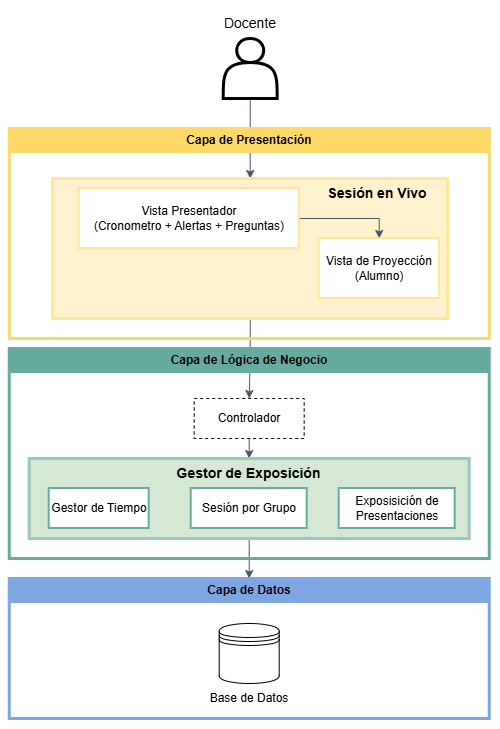
\includegraphics[width=0.9\textwidth]{TT-II/Fig01.png}
    \caption{Arquitectura del Prototipo 2.}
    \label{fig:arquitectura-prototipo-2}
\end{figure}
\FloatBarrier

\subsubsection*{Diagrama de componentes del Prototipo 2}
\addcontentsline{toc}{subsubsection}{\protect\ttiiTOC{Diagrama de componentes del Prototipo 2}}

El diagrama de componentes del prototipo 2 detalla la organización interna del módulo de exposición en aula a nivel de archivos de software, mostrando cómo se distribuyen las responsabilidades entre los componentes que lo conforman y las relaciones de uso entre ellos. A diferencia del prototipo 1, cuya capa de presentación agrupa componentes orientados a la carga y el análisis de presentaciones, el prototipo 2 reorganiza esta capa en torno a la sesión de exposición activa, incorporando los componentes necesarios para la gestión en tiempo real.

La capa de presentación se divide en dos módulos. El primero, \textit{Subject \& Content Management}, agrupa los componentes de la vista del docente durante la exposición: \texttt{presentation\_data\_panel.py}, que muestra los temporizadores, las preguntas y los datos de interés asociados a la diapositiva activa; \texttt{slides\_viewer\_panel.py}, que renderiza la diapositiva en curso dentro de la vista del presentador; y \texttt{presentation\_controls.py}, que gestiona los controles de navegación entre diapositivas y el botón para detener la exposición. Estos tres componentes son coordinados por \texttt{presentation\_gui.py}, que actúa como orquestador de la vista del docente. El segundo módulo, \textit{Proyection}, contiene únicamente \texttt{projection\_gui.py}, responsable de desplegar la vista del alumno en pantalla completa en el dispositivo de salida externo. Este componente recibe de \texttt{presentation\_gui.py} las instrucciones de cambio de diapositiva para mantener ambas vistas sincronizadas. La navegación entre el módulo de exposición y el resto del prototipo se gestiona mediante \texttt{navigator.py}.

La capa de lógica de negocio se concentra en el módulo \textit{Controller}, que en este prototipo agrupa dos controladores: \texttt{presentation\_controller.py}, encargado de coordinar el flujo de la sesión de exposición, incluyendo la gestión del grupo seleccionado, el registro de la diapositiva activa y la comunicación con la capa de datos; y \texttt{subject\_controller.py}, que proporciona la información de la unidad de aprendizaje asociada a la presentación en curso. A diferencia del prototipo 1, este prototipo no incorpora módulos de métricas en la capa de lógica de negocio, dado que el procesamiento analítico se completó en la etapa anterior.

La capa de infraestructura no introduce componentes nuevos en este prototipo, ya que el módulo de exposición en aula no requiere comunicación con la API de Google Gemini durante la sesión; los datos que se muestran fueron recuperados previamente por el módulo de análisis.

La capa de datos mantiene la misma estructura del prototipo anterior: \texttt{persistence.py} y \texttt{queries.py}, coordinados por \texttt{database\_manager.py}, que administra todas las operaciones sobre la base de datos \texttt{ai\_analyzer.db}. En este prototipo, las operaciones de persistencia se orientan al registro del avance por grupo, incluida la diapositiva de cierre y los tiempos por diapositiva, para su uso posterior en el informe de rendimiento del prototipo 3.

La Figura \ref{fig:componentes-prototipo-2} presenta el diagrama de componentes descrito.

\begin{figure}[!htbp]
    \centering
    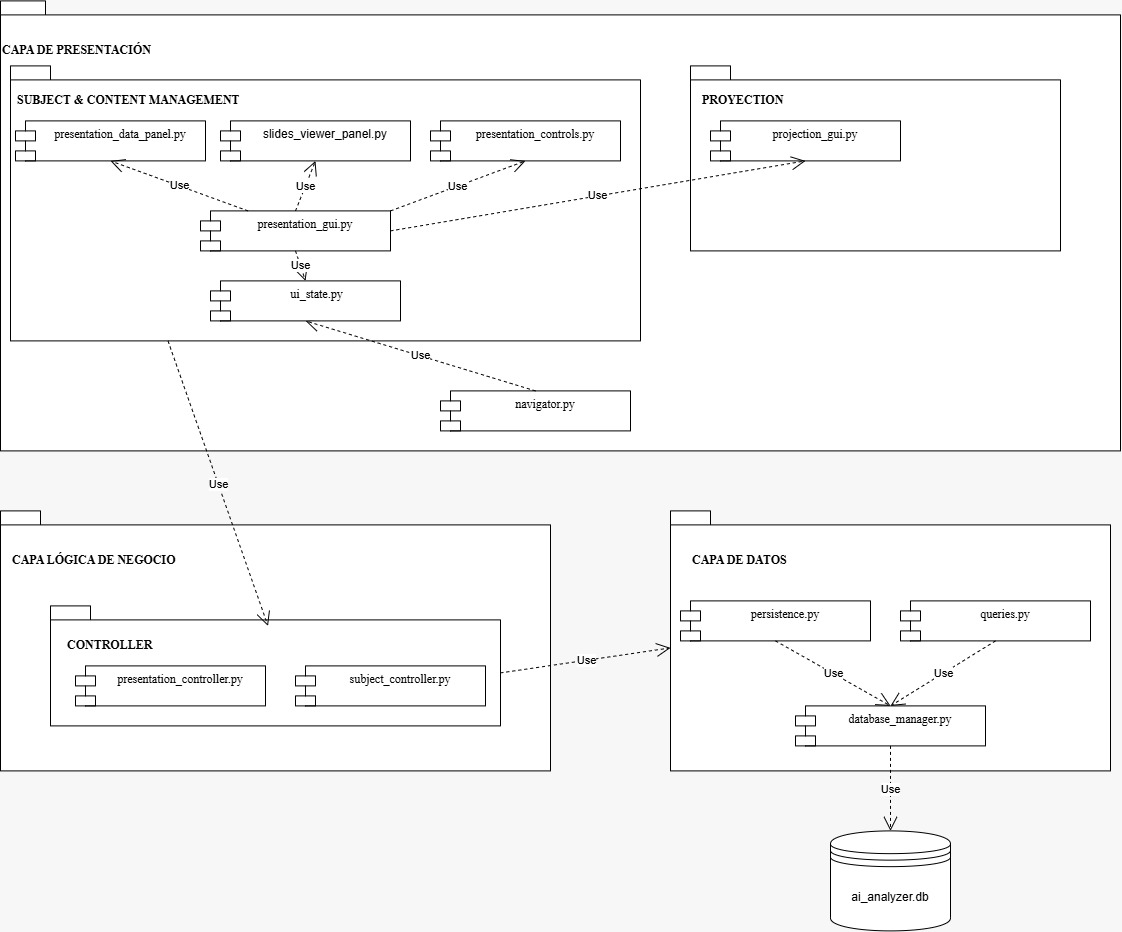
\includegraphics[width=0.95\textwidth]{TT-II/Fig02.jpeg}
    \caption{Diagrama de Componentes del Prototipo 2.}
    \label{fig:componentes-prototipo-2}
\end{figure}
\clearpage

\subsubsection*{Diseño de la interfaz del Prototipo 2}
\addcontentsline{toc}{subsubsection}{\protect\ttiiTOC{Diseño de la interfaz del Prototipo 2}}

Las interfaces que se presentan a continuación representan el flujo de interacción del docente durante la configuración, el inicio, el desarrollo y la finalización de una sesión de exposición. Estas capturas documentan la distribución visual de los elementos principales de cada pantalla, las validaciones aplicadas a los datos de configuración y la sincronización entre la vista del docente y la vista proyectada para los alumnos, y constituyen la referencia de la interfaz funcional implementada en el prototipo 2.

\begin{figure}[!htbp]
    \centering
    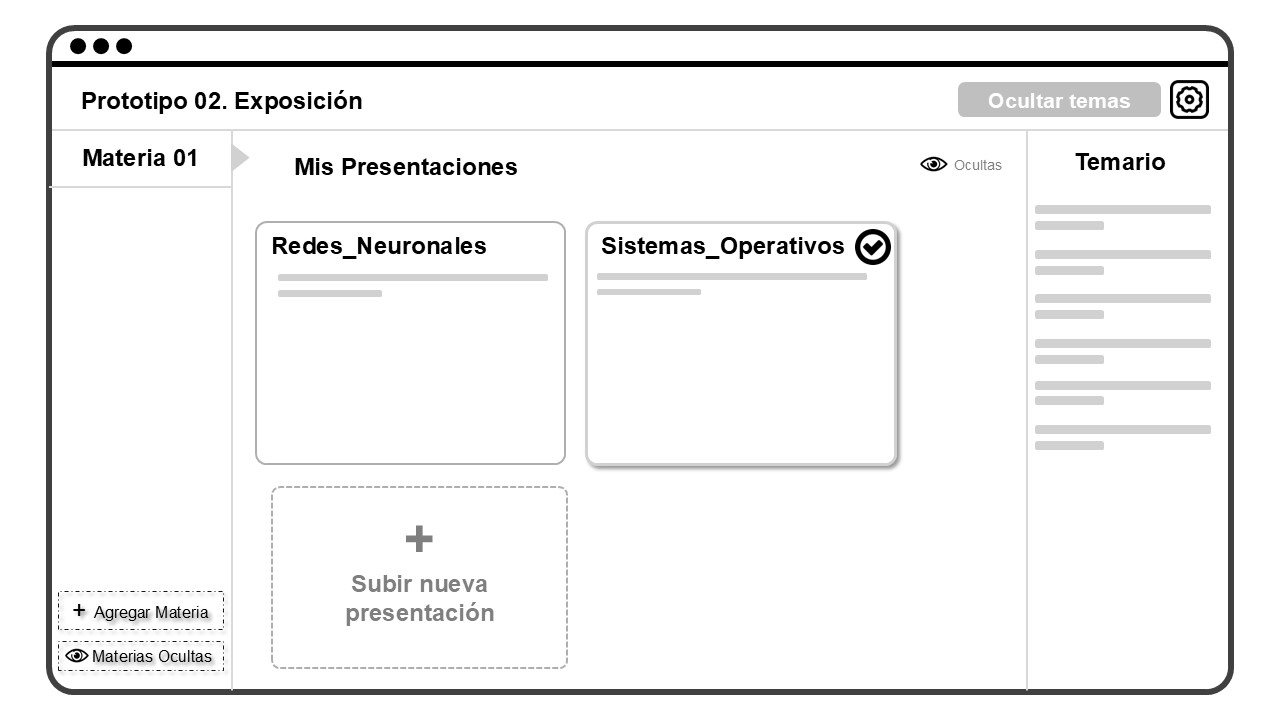
\includegraphics[width=0.8\textwidth]{TT-II/Fig03.JPG}
    \caption{Interfaz para la selección de una presentación analizada previamente.}
    \label{fig:interfaz-prototipo-2-03}
\end{figure}

\begin{figure}[!htbp]
    \centering
    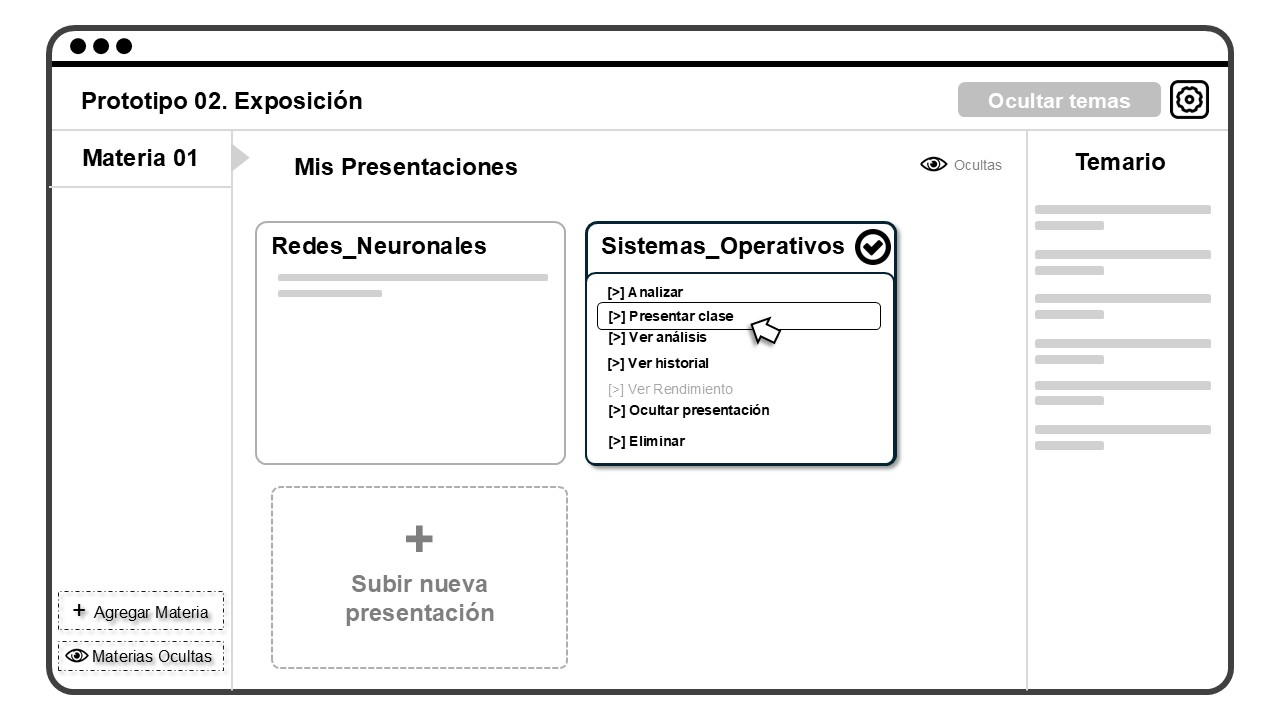
\includegraphics[width=0.8\textwidth]{TT-II/Fig04.JPG}
    \caption{Menú de acciones de la presentación con la opción \textit{Presentar clase}.}
    \label{fig:interfaz-prototipo-2-04}
\end{figure}

\begin{figure}[!htbp]
    \centering
    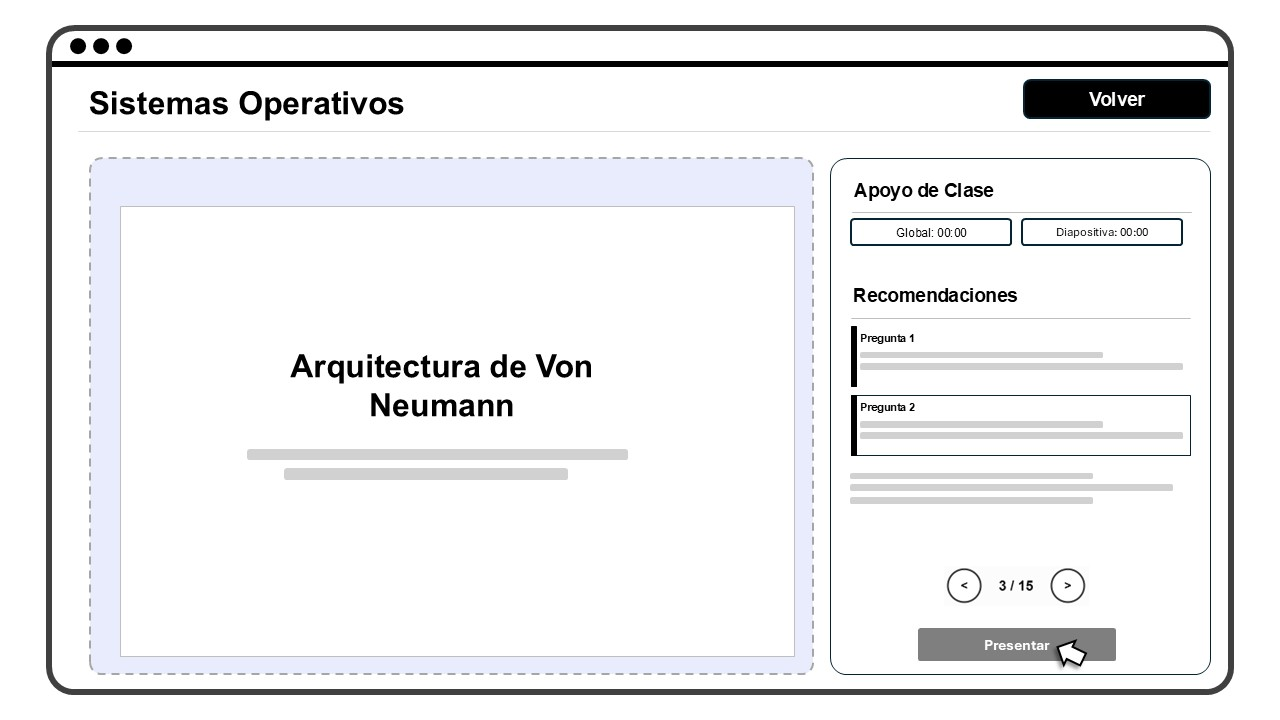
\includegraphics[width=0.8\textwidth]{TT-II/Fig05.JPG}
    \caption{Vista previa de la interfaz del docente antes de iniciar la exposición.}
    \label{fig:interfaz-prototipo-2-05}
\end{figure}

\begin{figure}[!htbp]
    \centering
    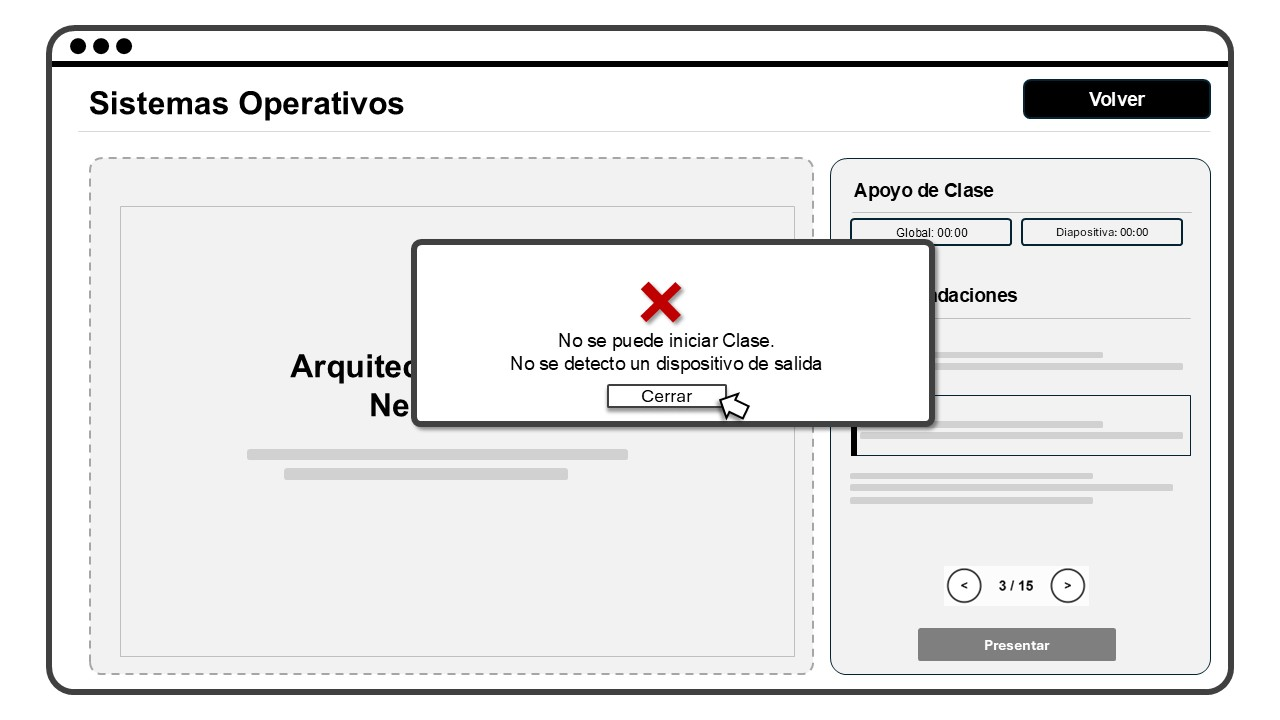
\includegraphics[width=0.8\textwidth]{TT-II/Fig06.JPG}
    \caption{Mensaje de error por ausencia de un dispositivo de salida externo.}
    \label{fig:interfaz-prototipo-2-06}
\end{figure}

\begin{figure}[!htbp]
    \centering
    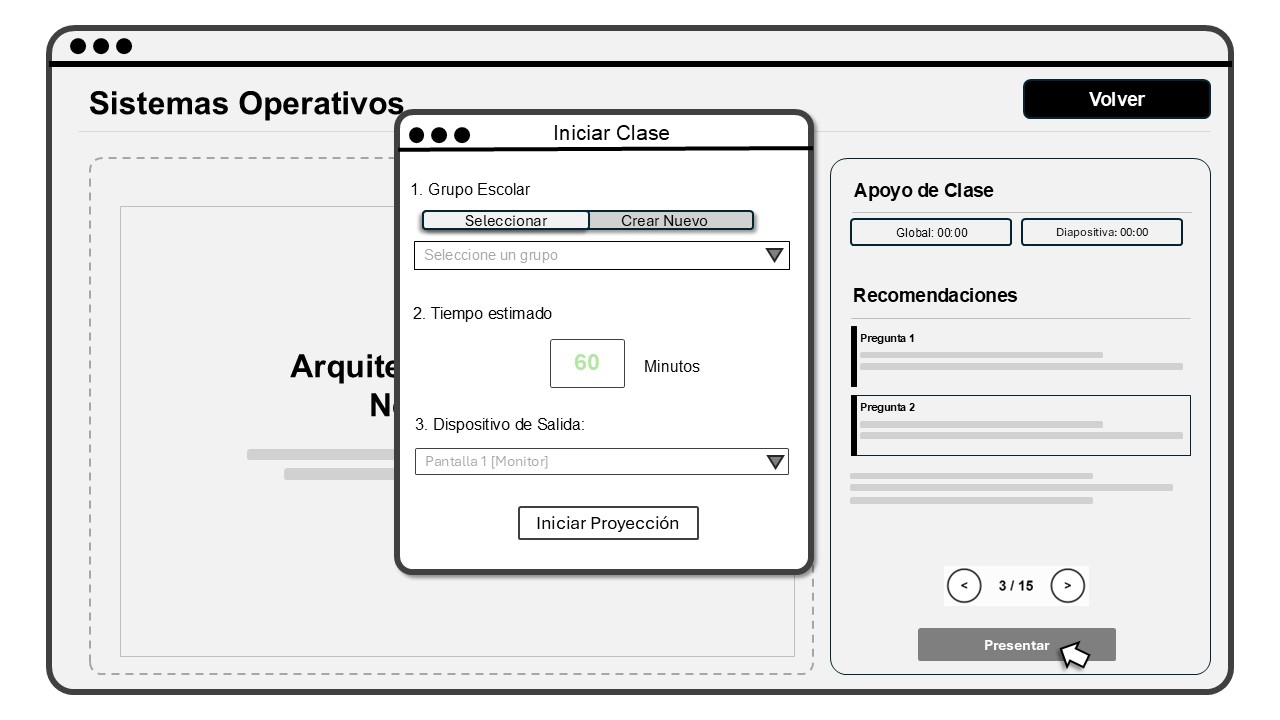
\includegraphics[width=0.8\textwidth]{TT-II/Fig07.JPG}
    \caption{Formulario de configuración de grupo, tiempo estimado y dispositivo de salida.}
    \label{fig:interfaz-prototipo-2-07}
\end{figure}

\begin{figure}[!htbp]
    \centering
    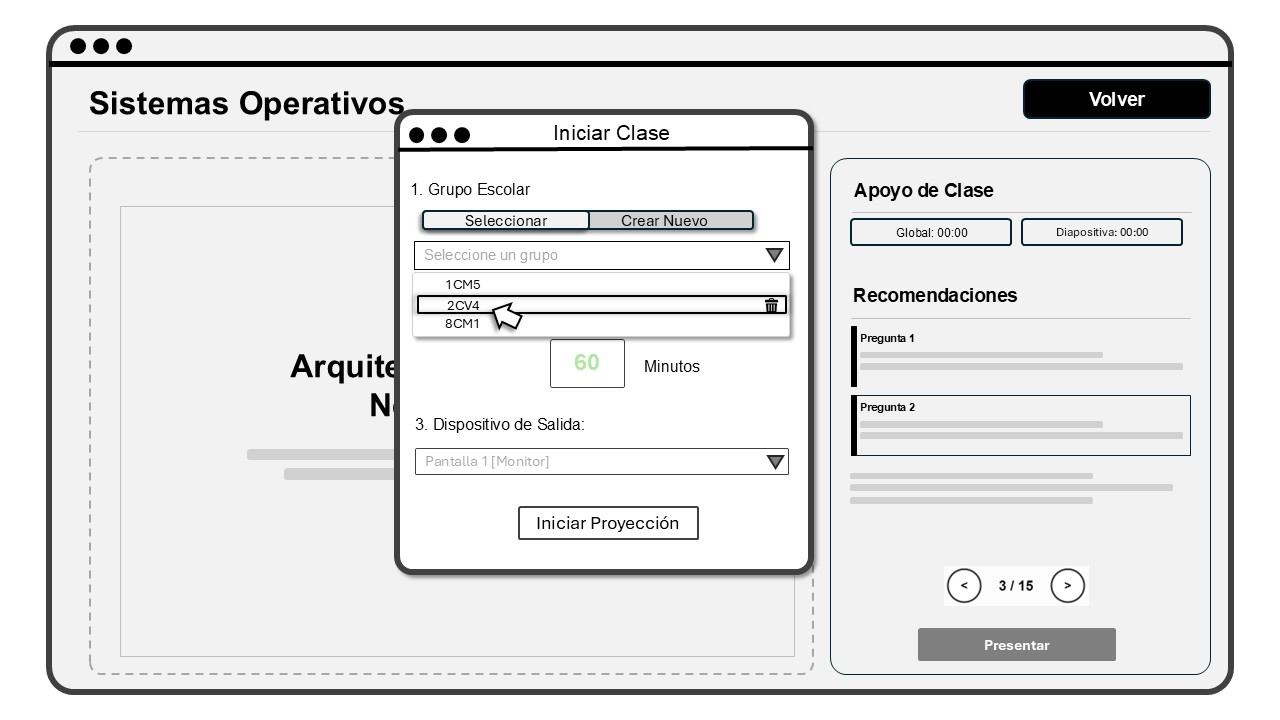
\includegraphics[width=0.8\textwidth]{TT-II/Fig08.JPG}
    \caption{Interfaz para la selección de un grupo registrado previamente.}
    \label{fig:interfaz-prototipo-2-08}
\end{figure}

\begin{figure}[!htbp]
    \centering
    \includegraphics[width=0.8\textwidth]{TT-II/Fig40.png}
    \caption{Interfaz para la eliminación de un grupo de exposición.}
    \label{fig:interfaz-prototipo-2-eliminacion-grupo}
\end{figure}

\begin{figure}[!htbp]
    \centering
    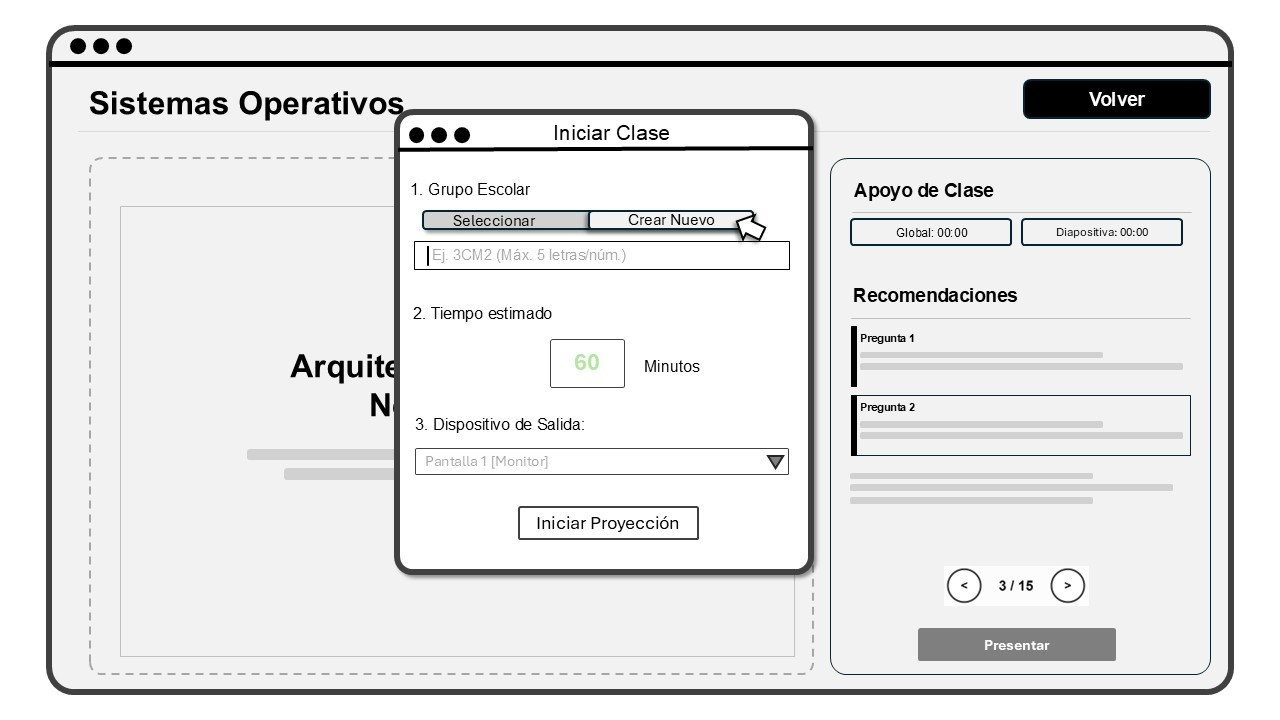
\includegraphics[width=0.8\textwidth]{TT-II/Fig09.JPG}
    \caption{Interfaz para la creación de un grupo con un máximo de cinco caracteres.}
    \label{fig:interfaz-prototipo-2-09}
\end{figure}

\begin{figure}[!htbp]
    \centering
    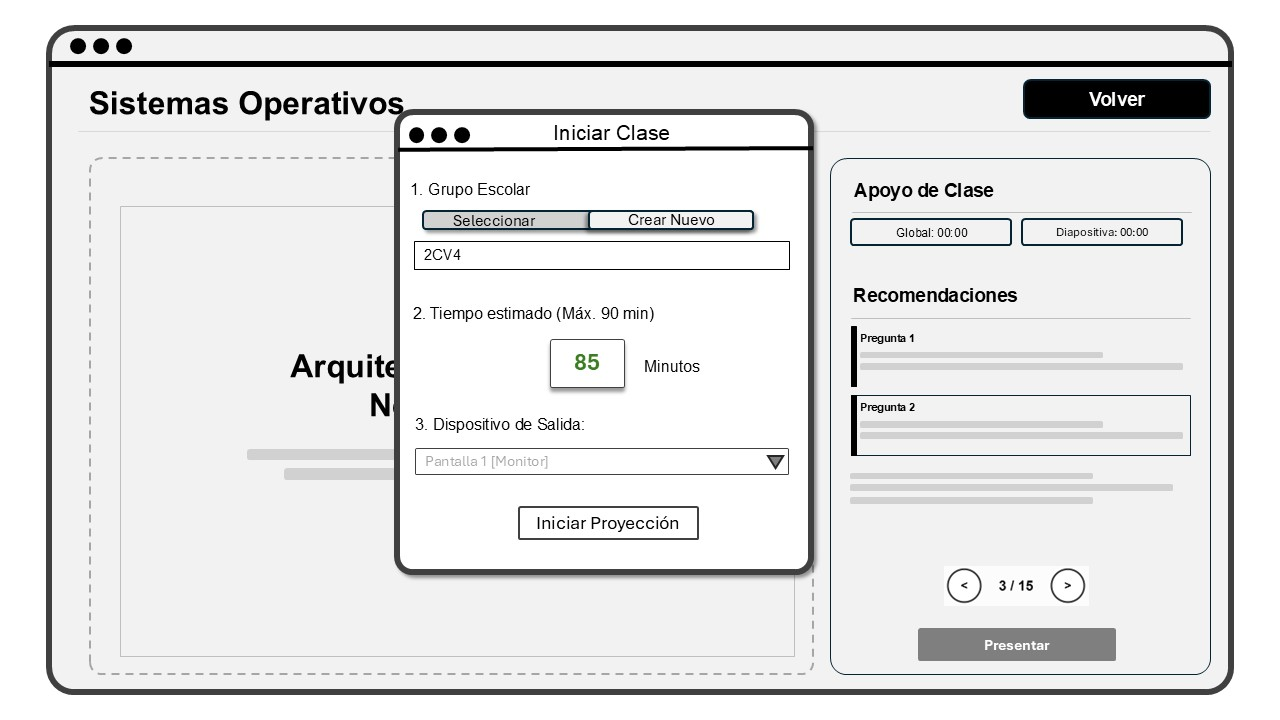
\includegraphics[width=0.8\textwidth]{TT-II/Fig10.JPG}
    \caption{Configuración del tiempo estimado de exposición con valor predeterminado de 60 minutos.}
    \label{fig:interfaz-prototipo-2-10}
\end{figure}

\begin{figure}[!htbp]
    \centering
    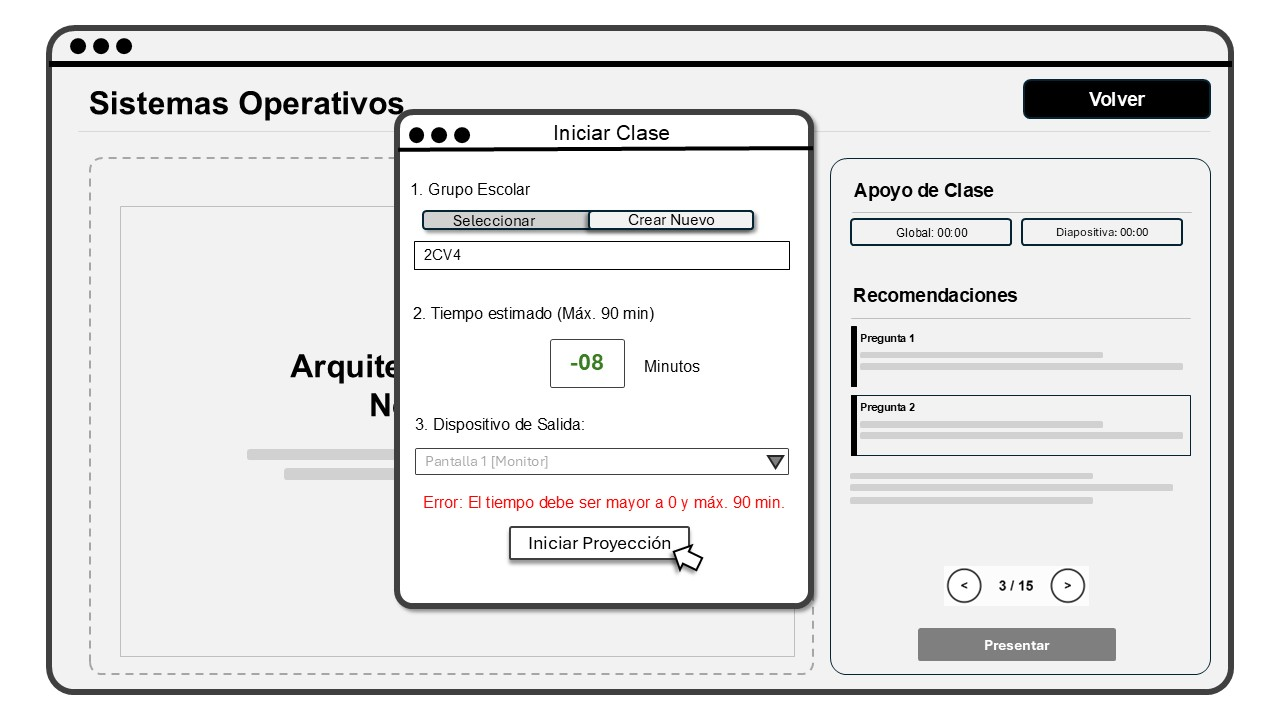
\includegraphics[width=0.8\textwidth]{TT-II/Fig11.JPG}
    \caption{Mensaje de error por ingresar un tiempo estimado fuera del intervalo de 1 a 90 minutos.}
    \label{fig:interfaz-prototipo-2-11}
\end{figure}

\begin{figure}[!htbp]
    \centering
    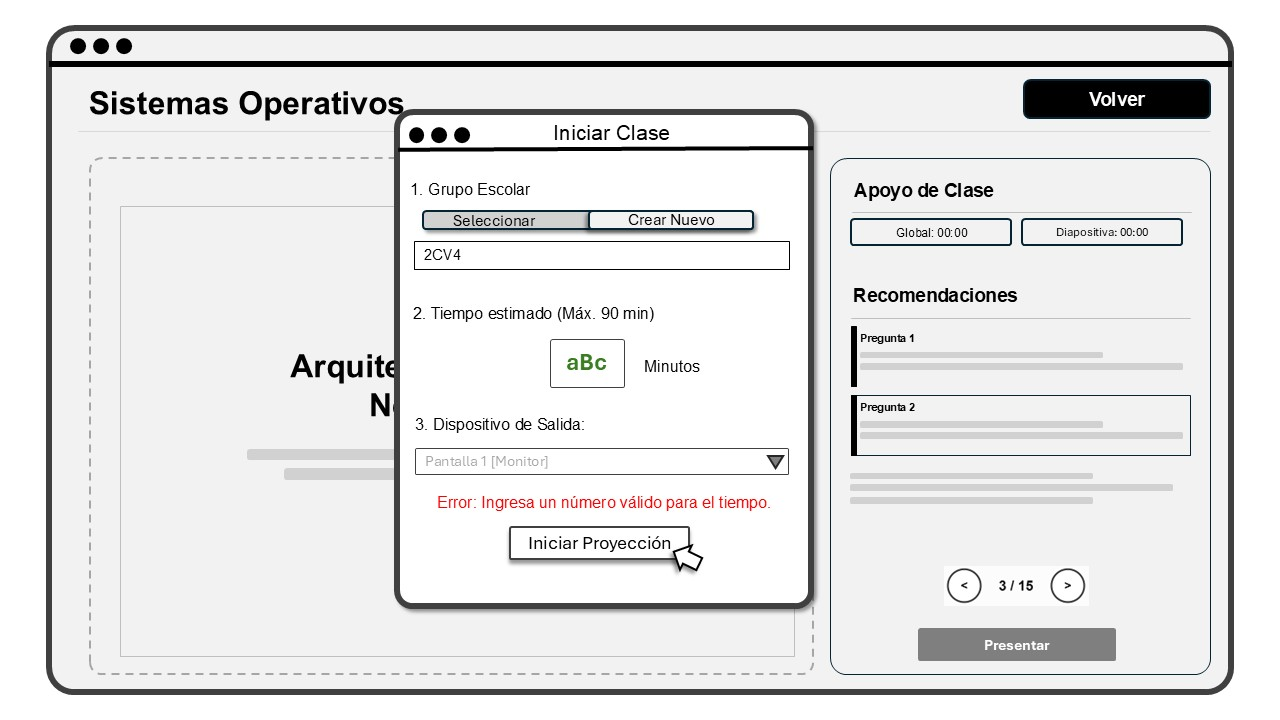
\includegraphics[width=0.8\textwidth]{TT-II/Fig12.JPG}
    \caption{Mensaje de error por ingresar caracteres no numéricos en el tiempo estimado.}
    \label{fig:interfaz-prototipo-2-12}
\end{figure}

\begin{figure}[!htbp]
    \centering
    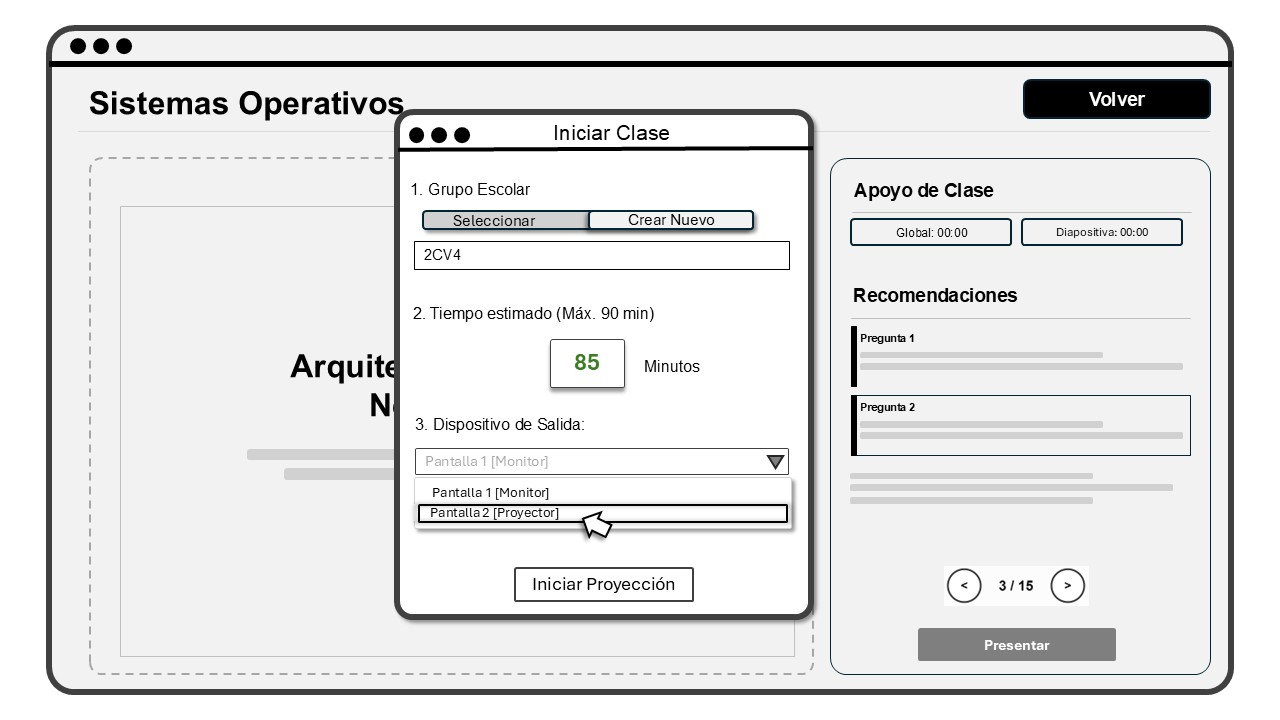
\includegraphics[width=0.8\textwidth]{TT-II/Fig13.JPG}
    \caption{Selección del primer dispositivo de salida detectado como opción predeterminada.}
    \label{fig:interfaz-prototipo-2-13}
\end{figure}

\begin{figure}[!htbp]
    \centering
    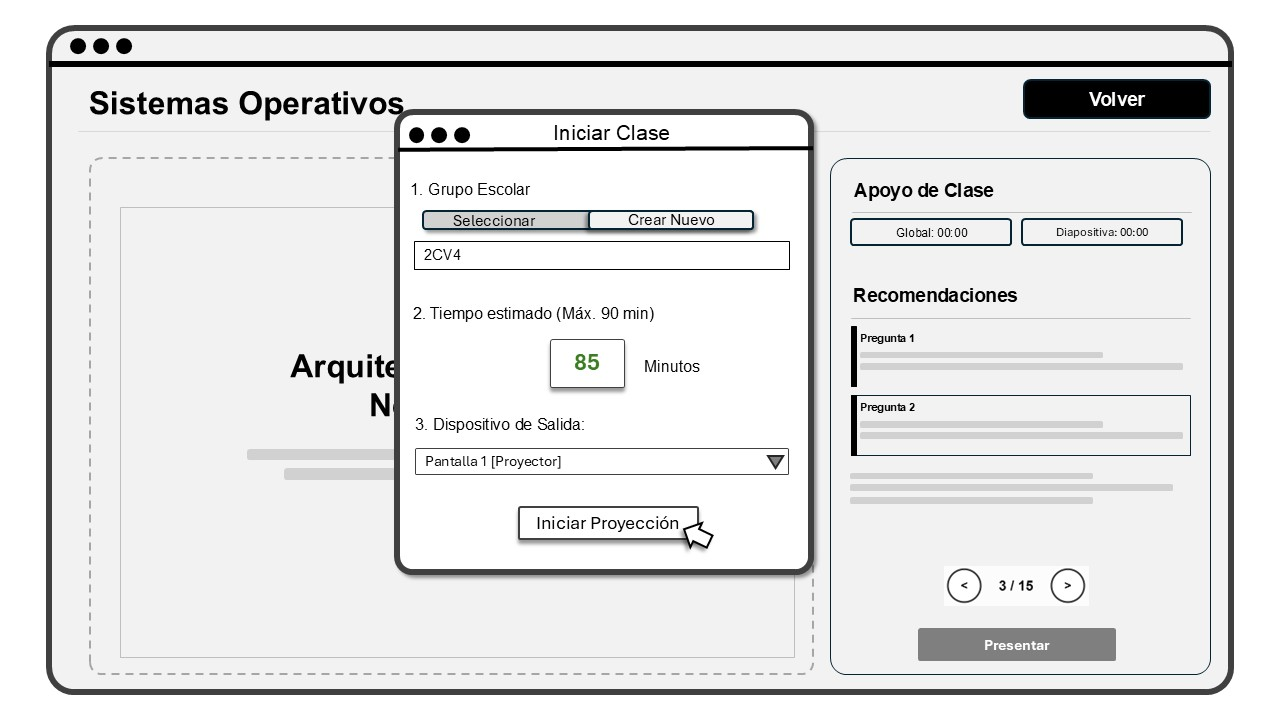
\includegraphics[width=0.8\textwidth]{TT-II/Fig14.JPG}
    \caption{Habilitación del inicio de la exposición tras completar correctamente el formulario.}
    \label{fig:interfaz-prototipo-2-14}
\end{figure}

\begin{figure}[!htbp]
    \centering
    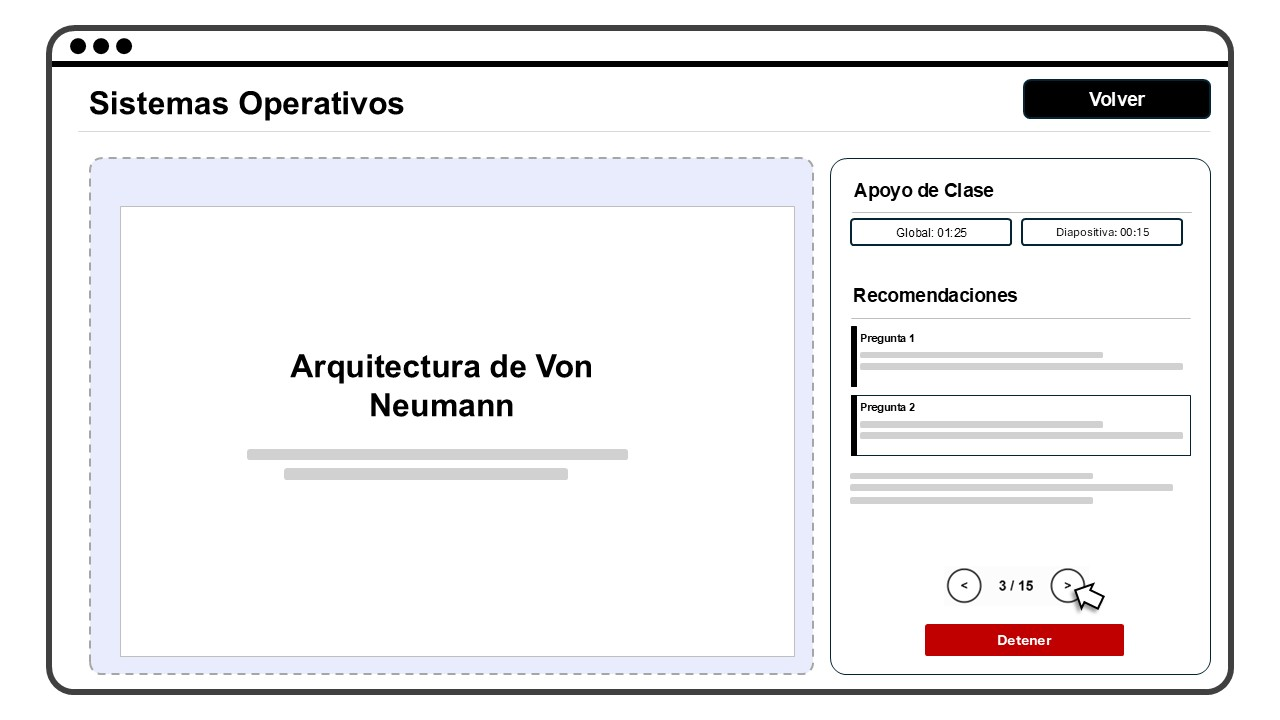
\includegraphics[width=0.8\textwidth]{TT-II/Fig15.JPG}
    \caption{Vista del docente durante la exposición con temporizadores y datos complementarios.}
    \label{fig:interfaz-prototipo-2-15}
\end{figure}

\begin{figure}[!htbp]
    \centering
    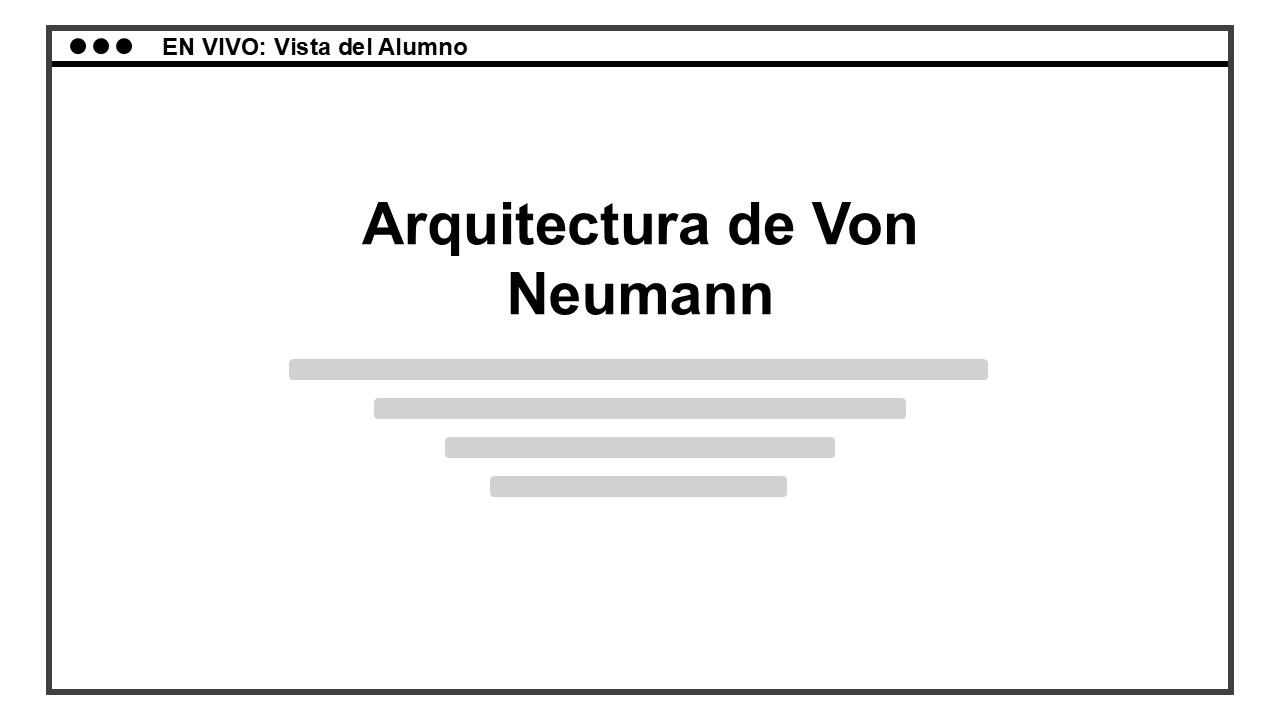
\includegraphics[width=0.8\textwidth]{TT-II/Fig16.JPG}
    \caption{Vista del alumno en el dispositivo de salida sin controles ni elementos adicionales.}
    \label{fig:interfaz-prototipo-2-16}
\end{figure}

\begin{figure}[!htbp]
    \centering
    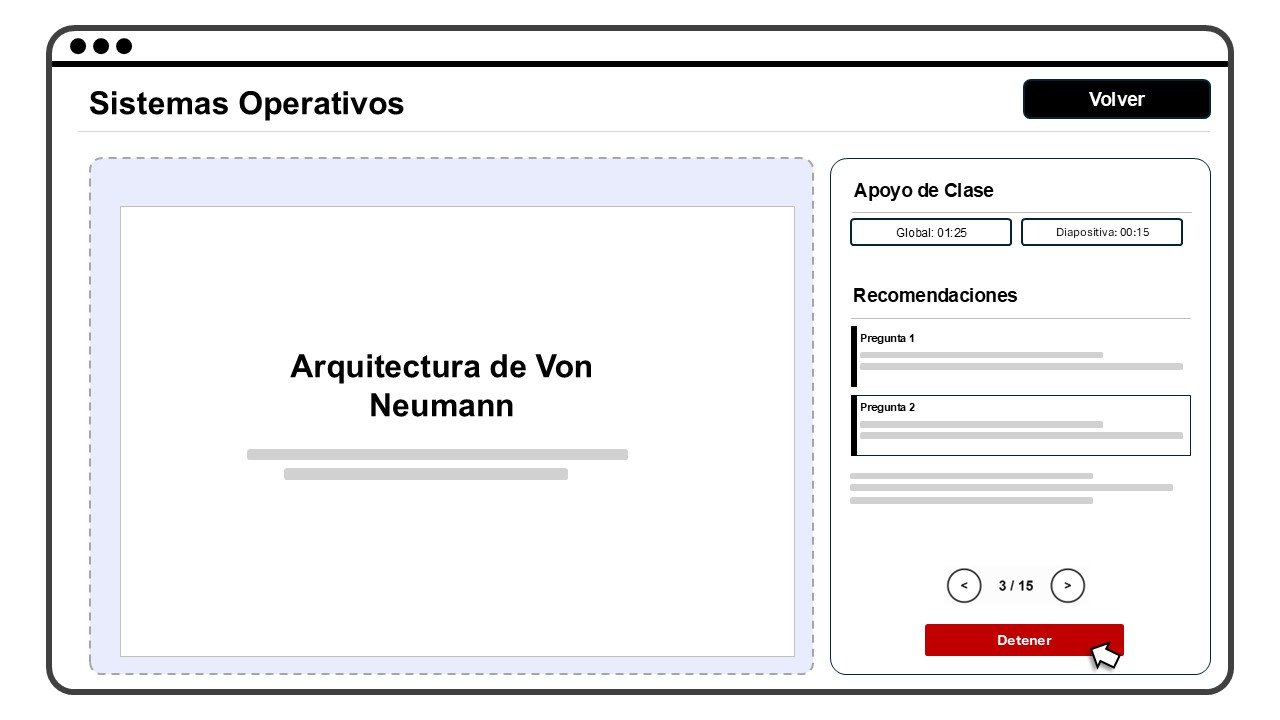
\includegraphics[width=0.8\textwidth]{TT-II/Fig17.JPG}
    \caption{Control para detener la exposición y registrar la última diapositiva mostrada.}
    \label{fig:interfaz-prototipo-2-17}
\end{figure}

\begin{figure}[!htbp]
    \centering
    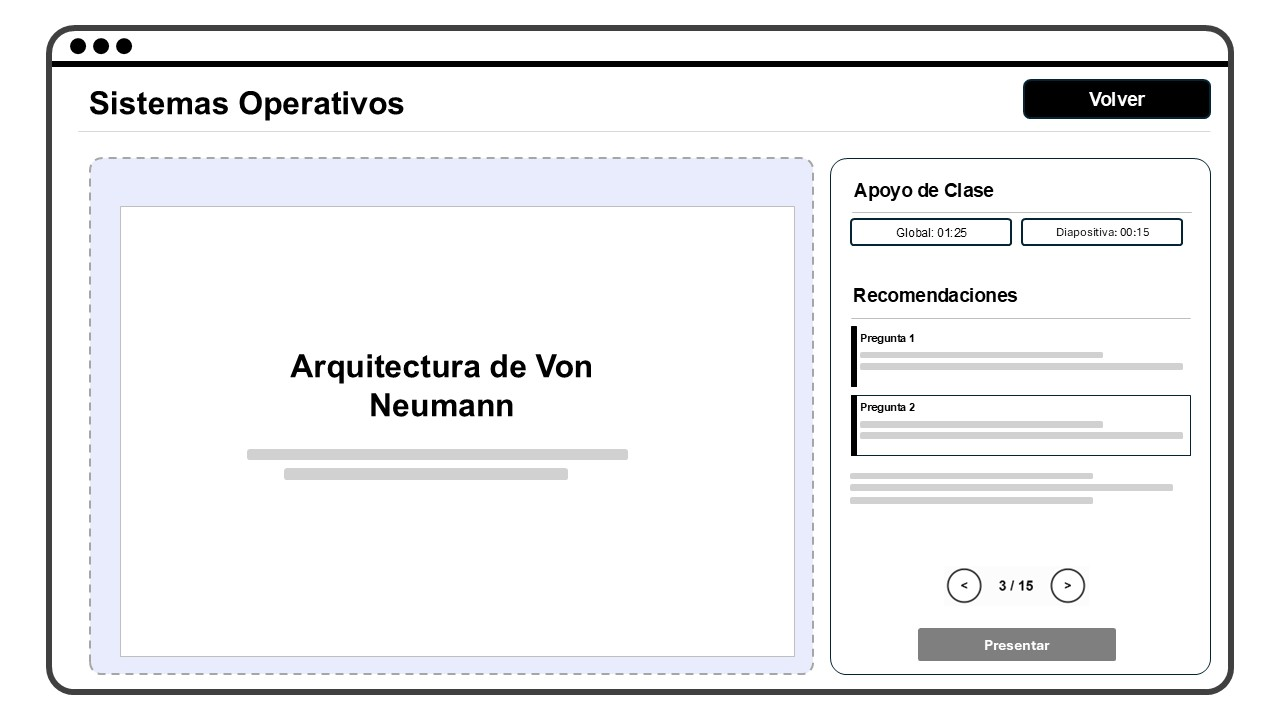
\includegraphics[width=0.8\textwidth]{TT-II/Fig18.JPG}
    \caption{Vista previa del docente después de detener la exposición, con la diapositiva y los tiempos registrados.}
    \label{fig:interfaz-prototipo-2-18}
\end{figure}

\begin{figure}[!htbp]
    \centering
    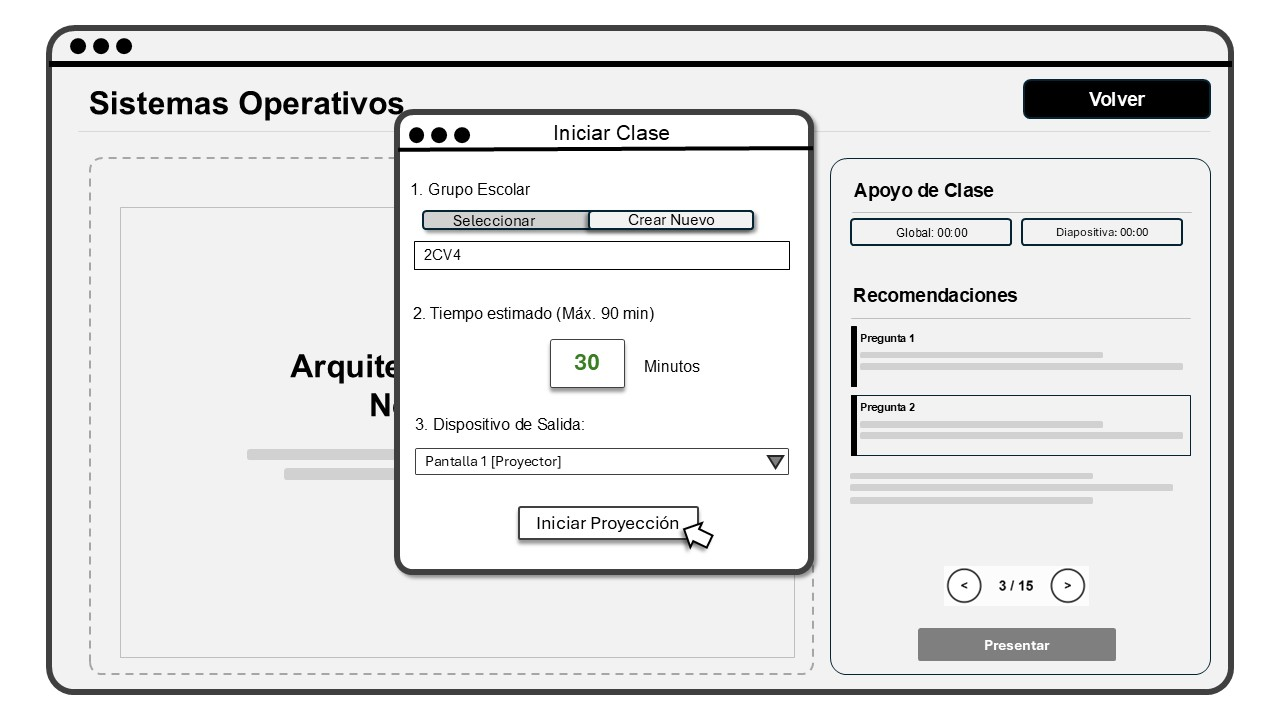
\includegraphics[width=0.8\textwidth]{TT-II/Fig19.JPG}
    \caption{Selección de un grupo con una sesión anterior registrada para la presentación.}
    \label{fig:interfaz-prototipo-2-19}
\end{figure}

\begin{figure}[!htbp]
    \centering
    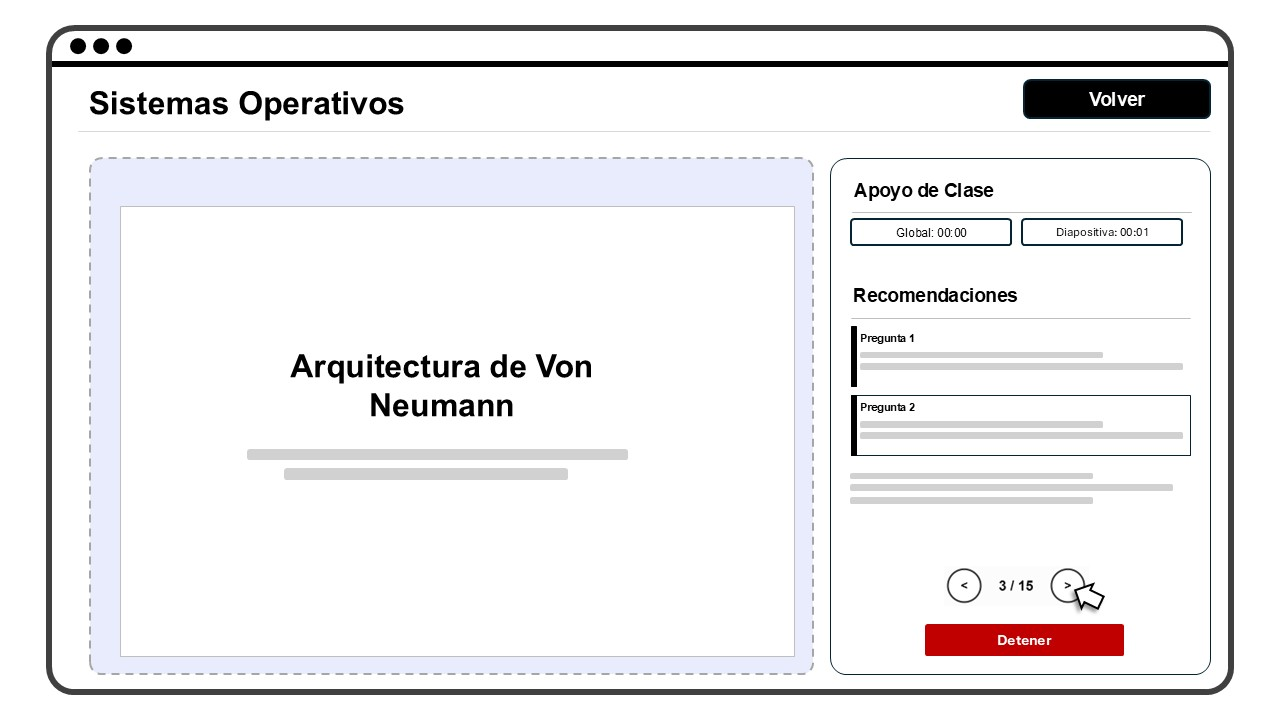
\includegraphics[width=0.8\textwidth]{TT-II/Fig20.JPG}
    \caption{Reanudación de la exposición desde la última diapositiva registrada y con los temporizadores reiniciados.}
    \label{fig:interfaz-prototipo-2-20}
\end{figure}

\begin{figure}[!htbp]
    \centering
    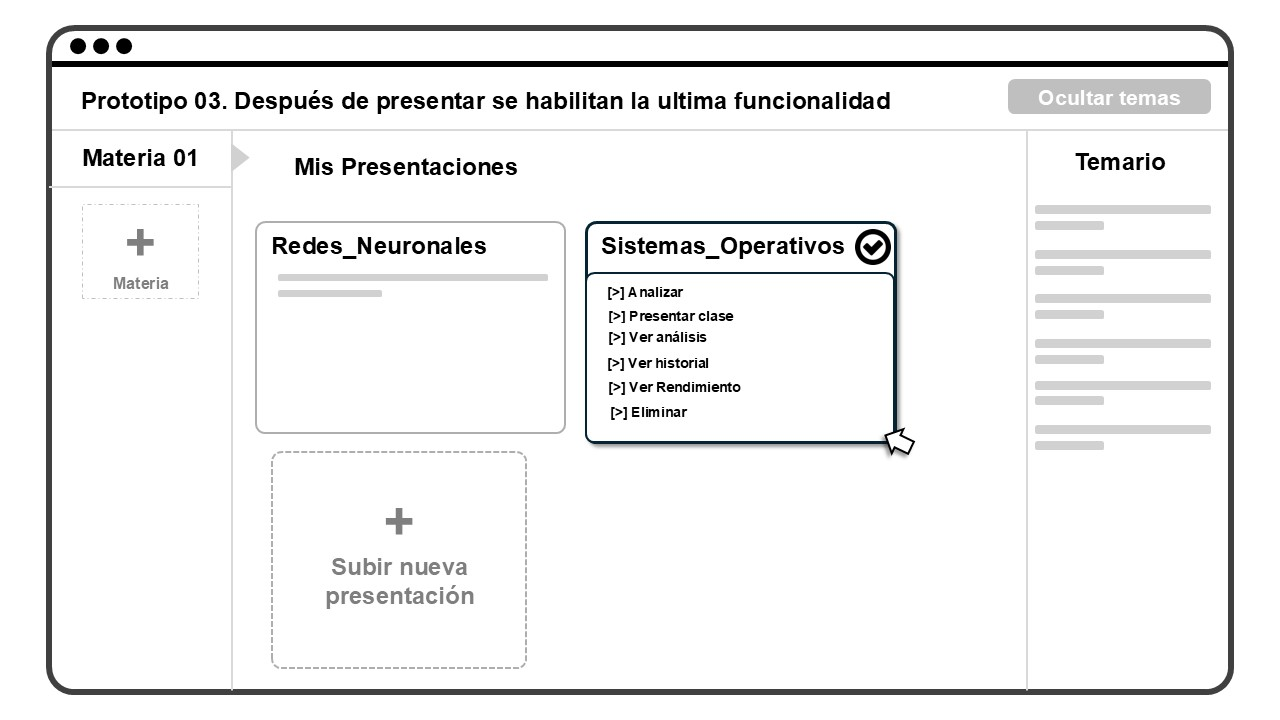
\includegraphics[width=0.8\textwidth]{TT-II/Fig21.JPG}
    \caption{Menú principal con la opción de consulta de rendimiento habilitada al finalizar la exposición.}
    \label{fig:interfaz-prototipo-2-21}
\end{figure}

\clearpage
\subsubsection*{Desarrollo del Prototipo 2}
\addcontentsline{toc}{subsubsection}{\protect\ttiiTOC{Desarrollo del Prototipo 2}}

La fase de desarrollo del prototipo 2 comprende la implementación de los módulos definidos en la arquitectura de cuatro capas descrita en la sección anterior, abarcando desde la configuración de la sesión de exposición y la gestión de grupos hasta la sincronización en tiempo real de las dos vistas, el monitoreo de temporizadores y el registro de los datos de la sesión para su uso posterior en el informe de rendimiento.

Con el propósito de documentar el comportamiento del prototipo 2 e ilustrar la interacción entre sus componentes durante la ejecución de los flujos principales, se elaboraron diagramas de secuencia para cada una de las funcionalidades centrales del módulo de exposición en aula.

Los flujos documentados mediante diagramas de secuencia corresponden a las siguientes operaciones: inicio de clase y ensamblaje de la vista del presentador, configuración de la sesión mediante el formulario modal de grupo y tiempo estimado, lanzamiento de la proyección y activación del mecanismo de vigilancia de la sesión, interacción en vivo con navegación sincronizada entre la vista del docente y la vista del alumno, detención de la exposición y persistencia de los tiempos registrados por diapositiva, y salida de la vista con restauración del estado anterior del prototipo. Cada diagrama contempla tanto el flujo principal de éxito como las variantes de excepción más relevantes, entre las que se incluyen la ausencia de dispositivo de salida externo al momento de iniciar la sesión.

\begin{figure}[!htbp]
    \centering
    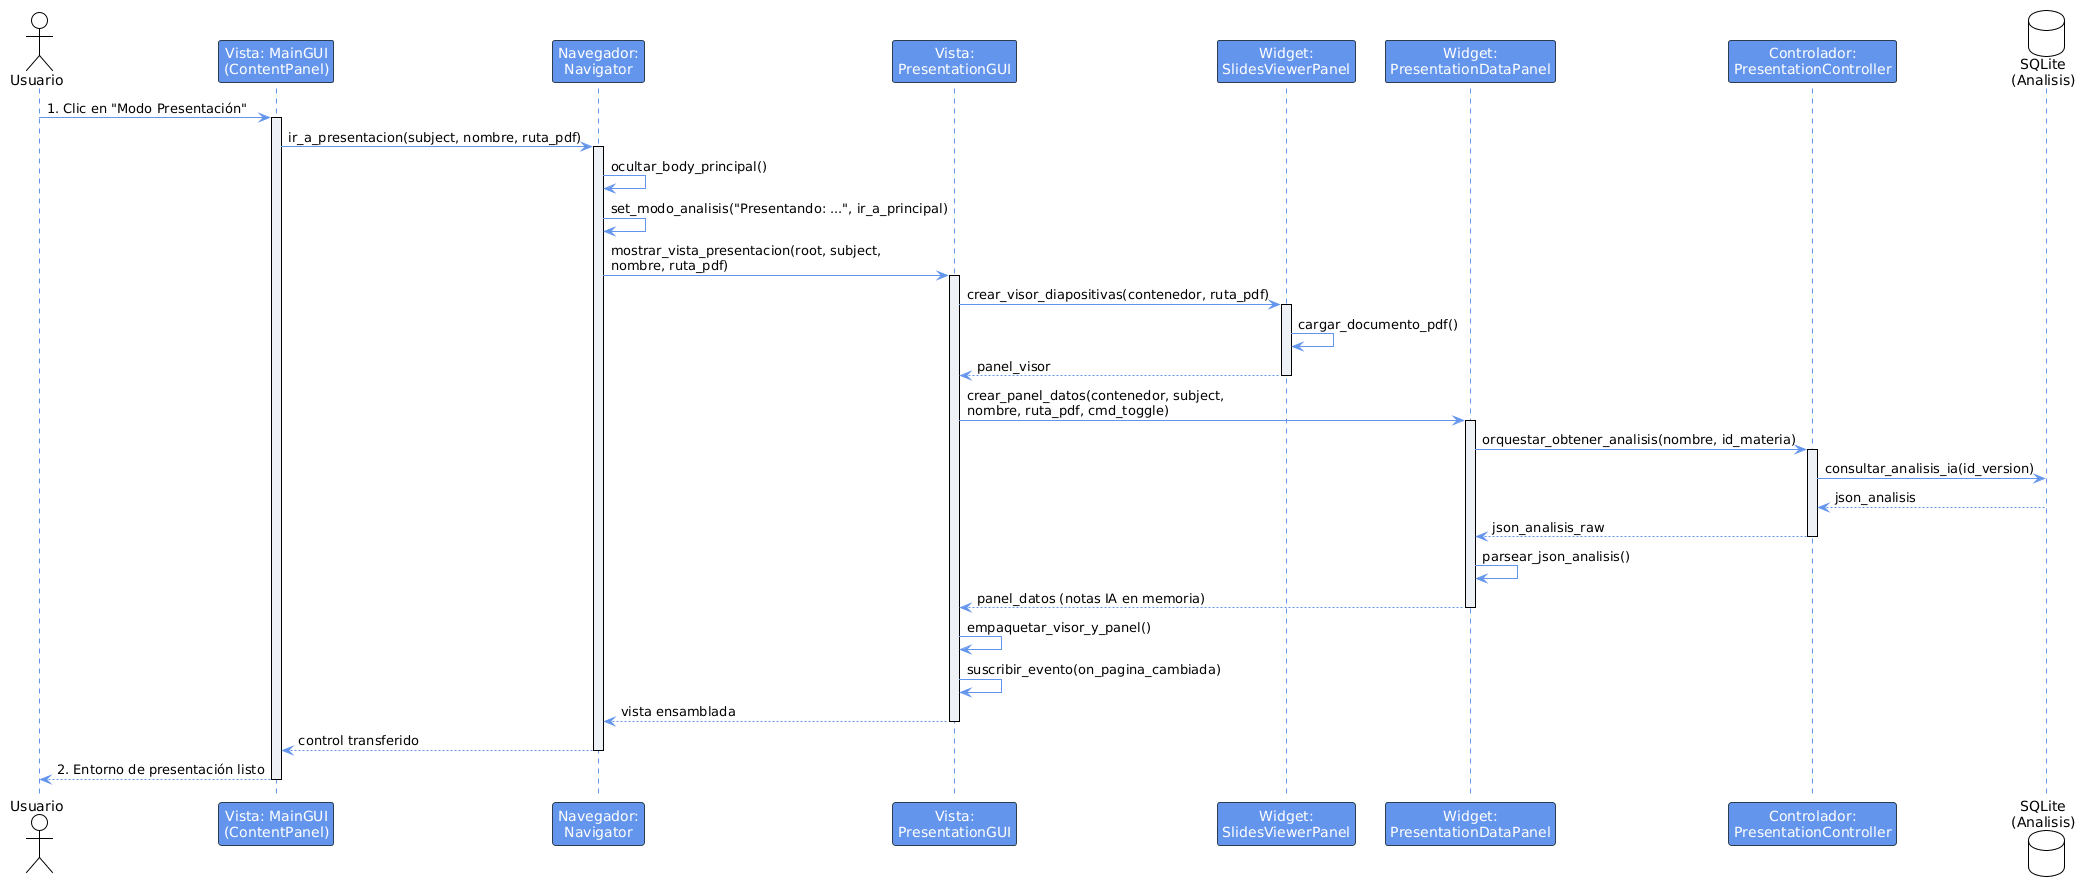
\includegraphics[width=0.95\textwidth]{TT-II/Fig22.png}
    \caption{Diagrama de secuencia del inicio de clase y ensamblaje de la vista.}
    \label{fig:secuencia-prototipo-2-inicio-clase}
\end{figure}

\begin{figure}[!htbp]
    \centering
    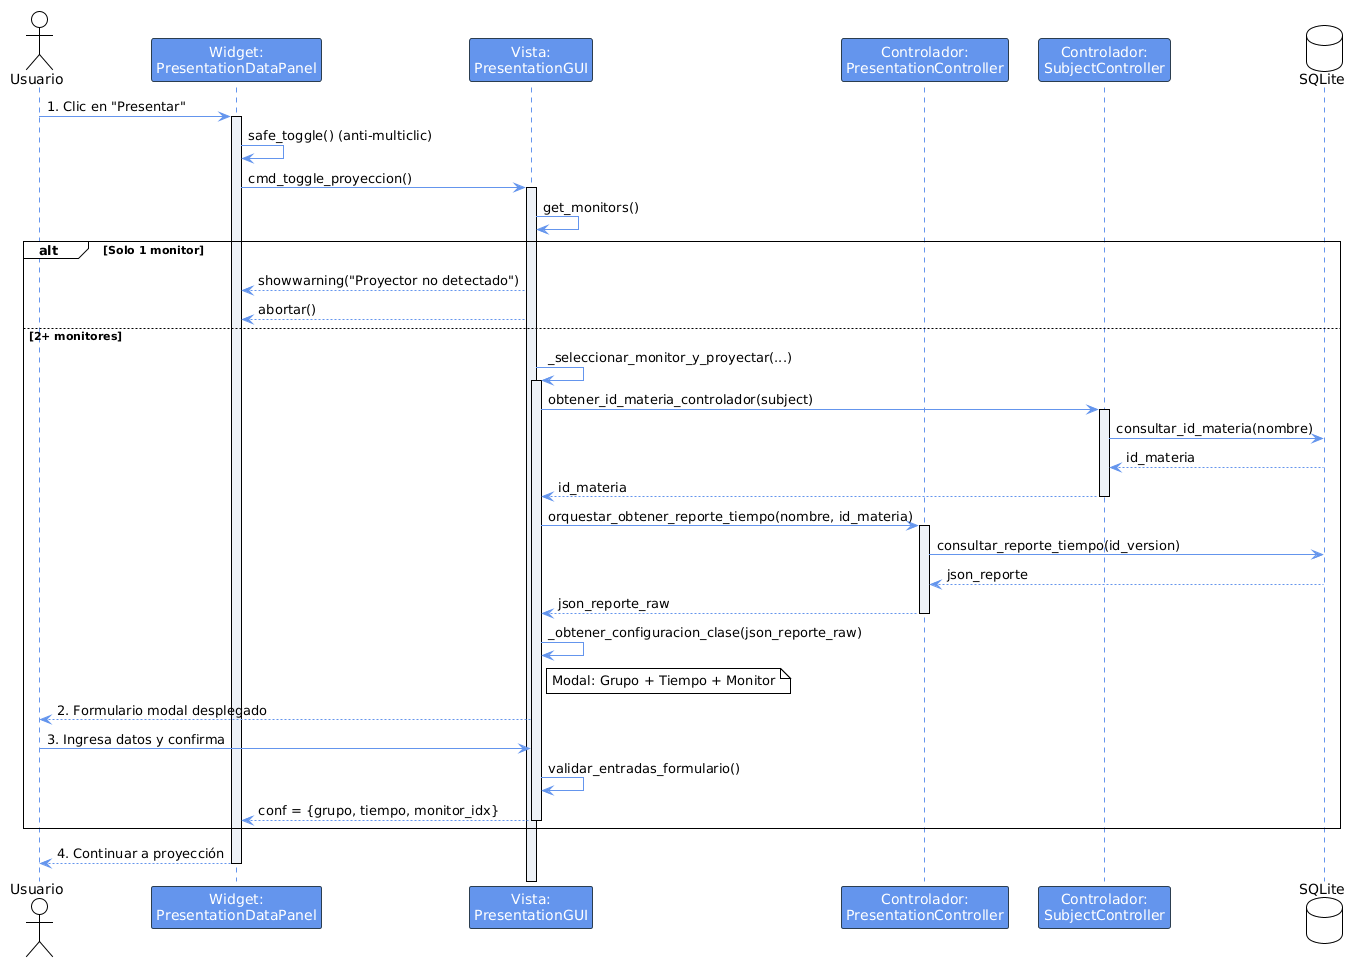
\includegraphics[width=0.95\textwidth]{TT-II/Fig23.png}
    \caption{Diagrama de secuencia de la configuración de sesión mediante el formulario modal.}
    \label{fig:secuencia-prototipo-2-configuracion-sesion}
\end{figure}

\begin{figure}[!htbp]
    \centering
    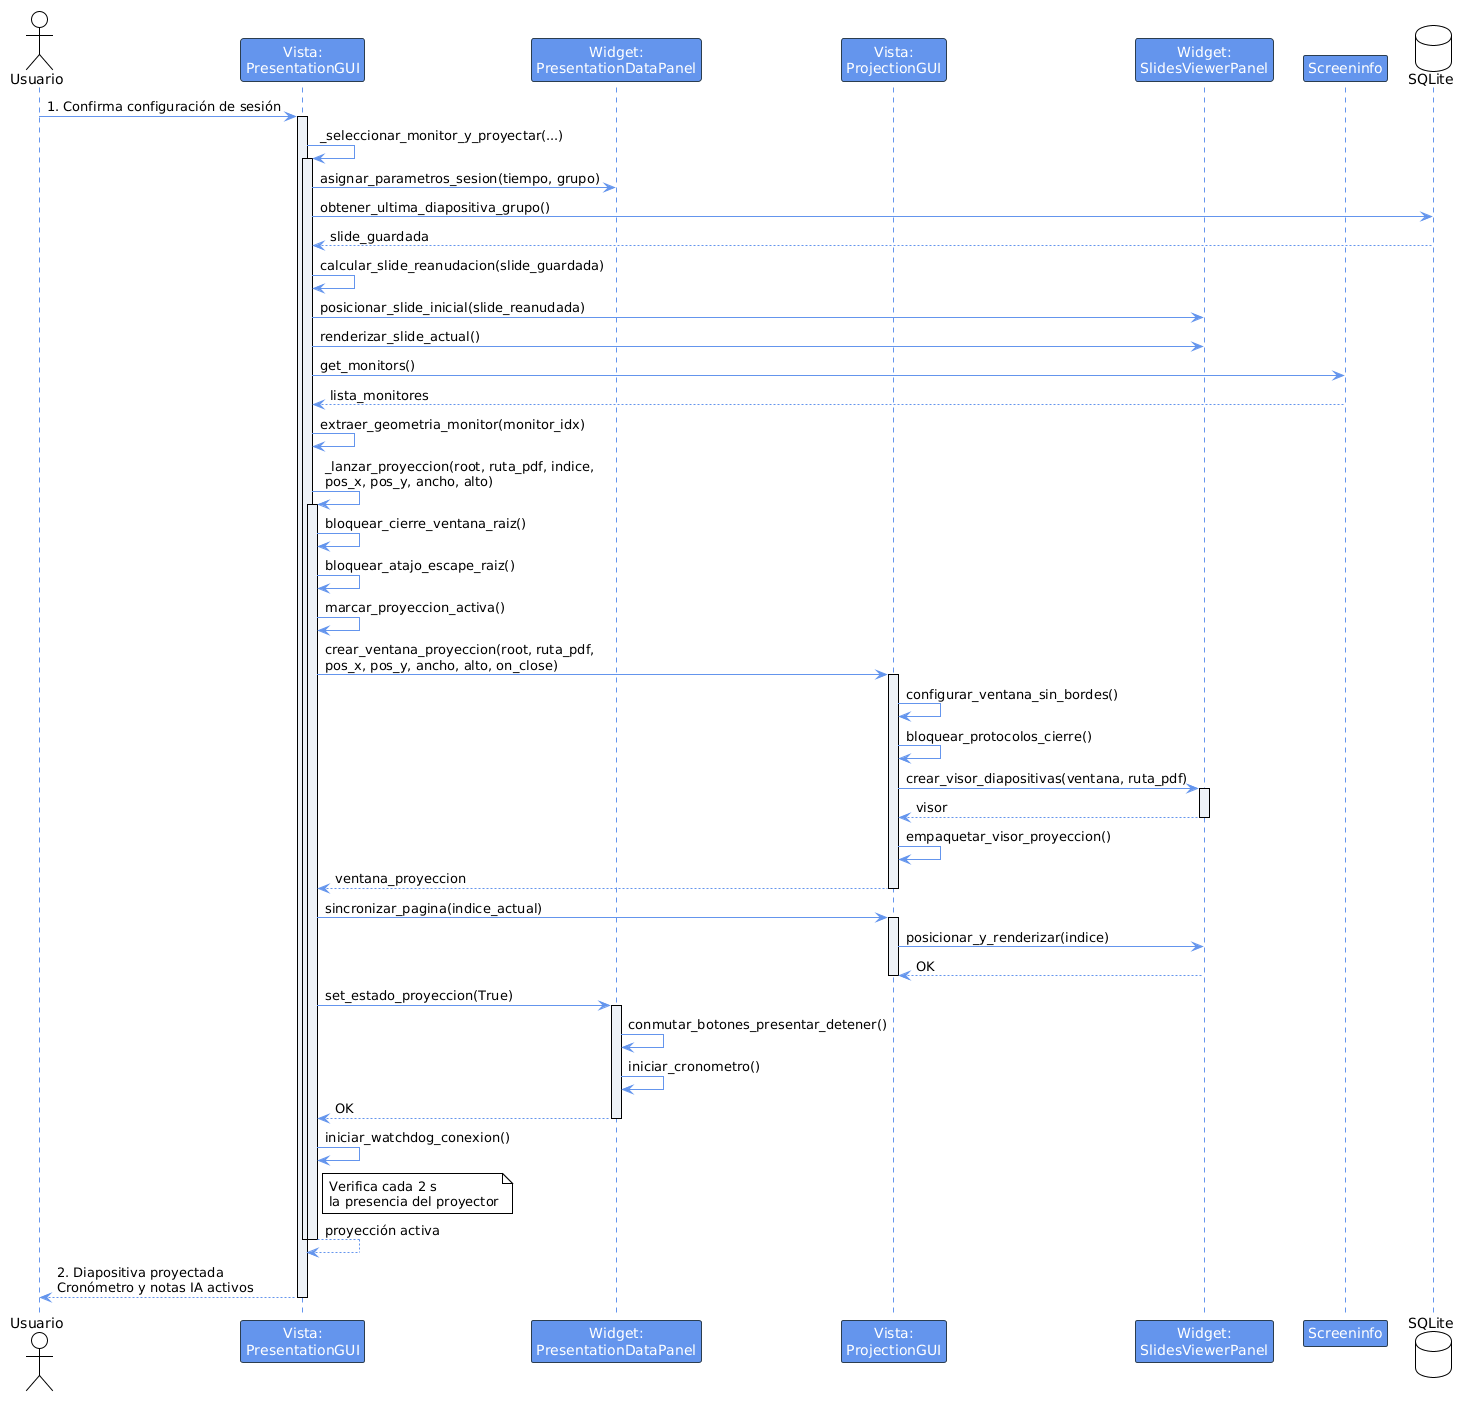
\includegraphics[width=0.95\textwidth]{TT-II/Fig24.png}
    \caption{Diagrama de secuencia del lanzamiento de la proyección y la activación del mecanismo de vigilancia.}
    \label{fig:secuencia-prototipo-2-lanzamiento-proyeccion}
\end{figure}

\begin{figure}[!htbp]
    \centering
    \includegraphics[width=0.95\textwidth]{TT-II/Fig41.png}
    \caption{Diagrama de secuencia de la eliminación de un grupo de exposición.}
    \label{fig:secuencia-prototipo-2-eliminacion-grupo}
\end{figure}

\begin{figure}[!htbp]
    \centering
    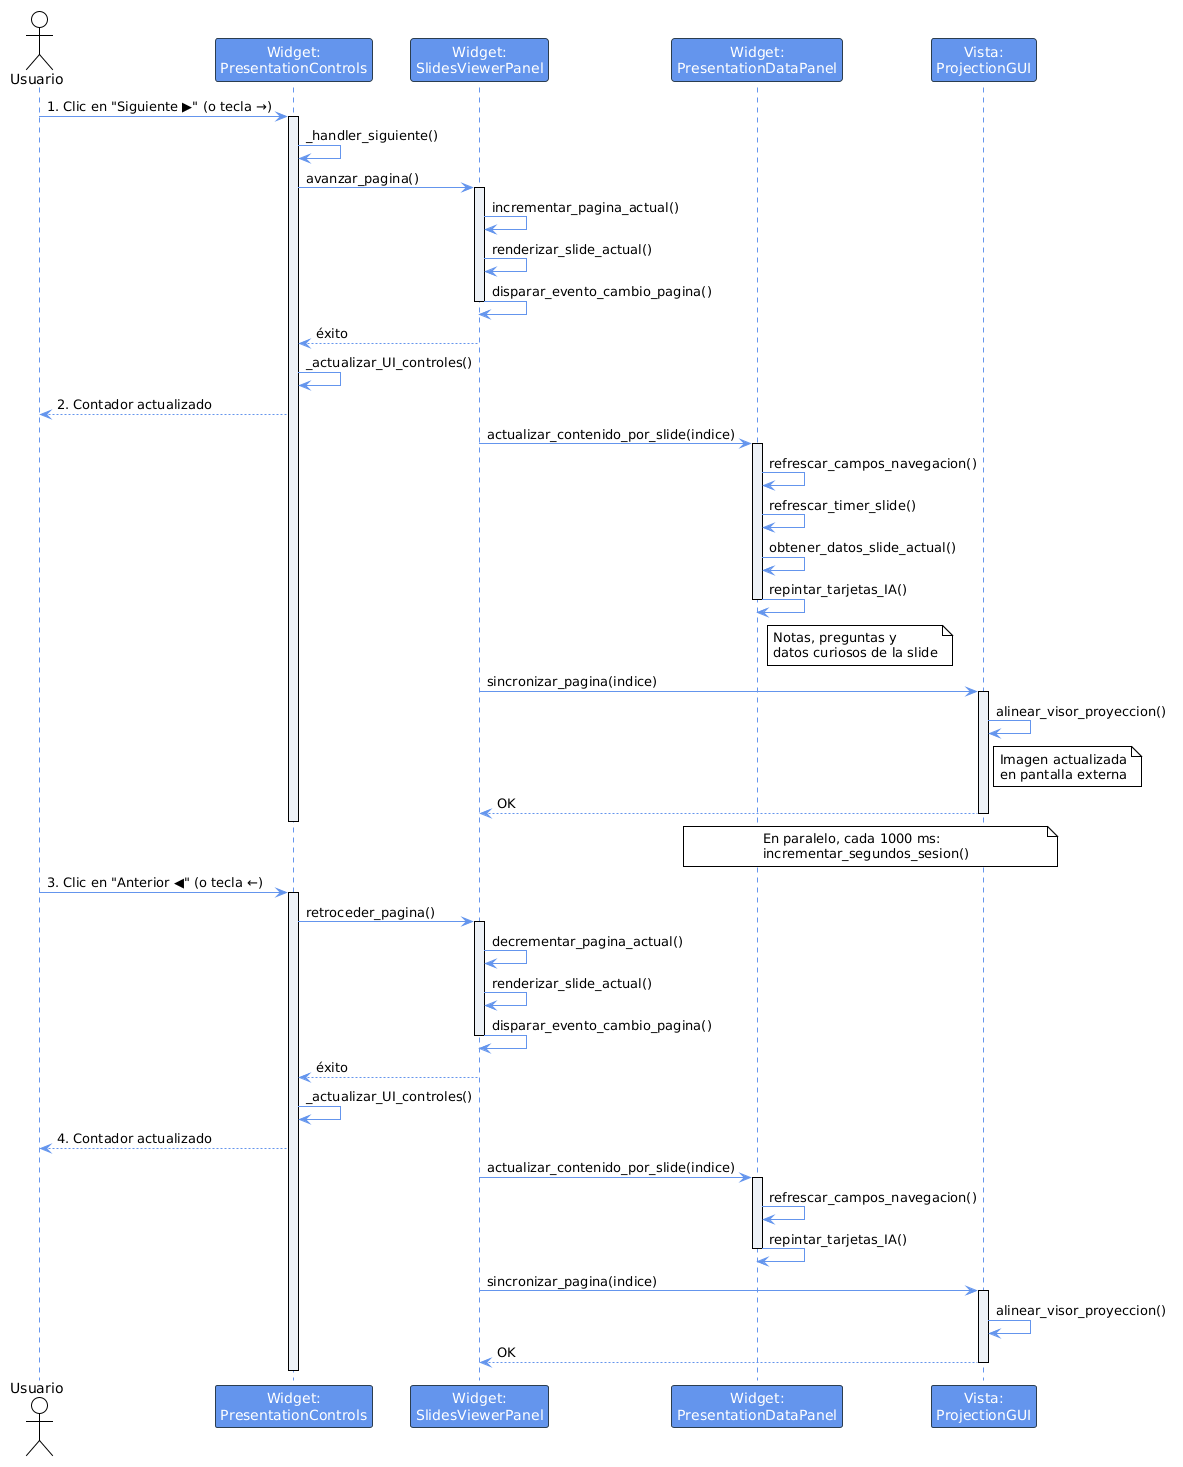
\includegraphics[width=0.95\textwidth]{TT-II/Fig25.png}
    \caption{Diagrama de secuencia de la interacción en vivo con navegación sincronizada.}
    \label{fig:secuencia-prototipo-2-interaccion-vivo}
\end{figure}

\begin{figure}[!htbp]
    \centering
    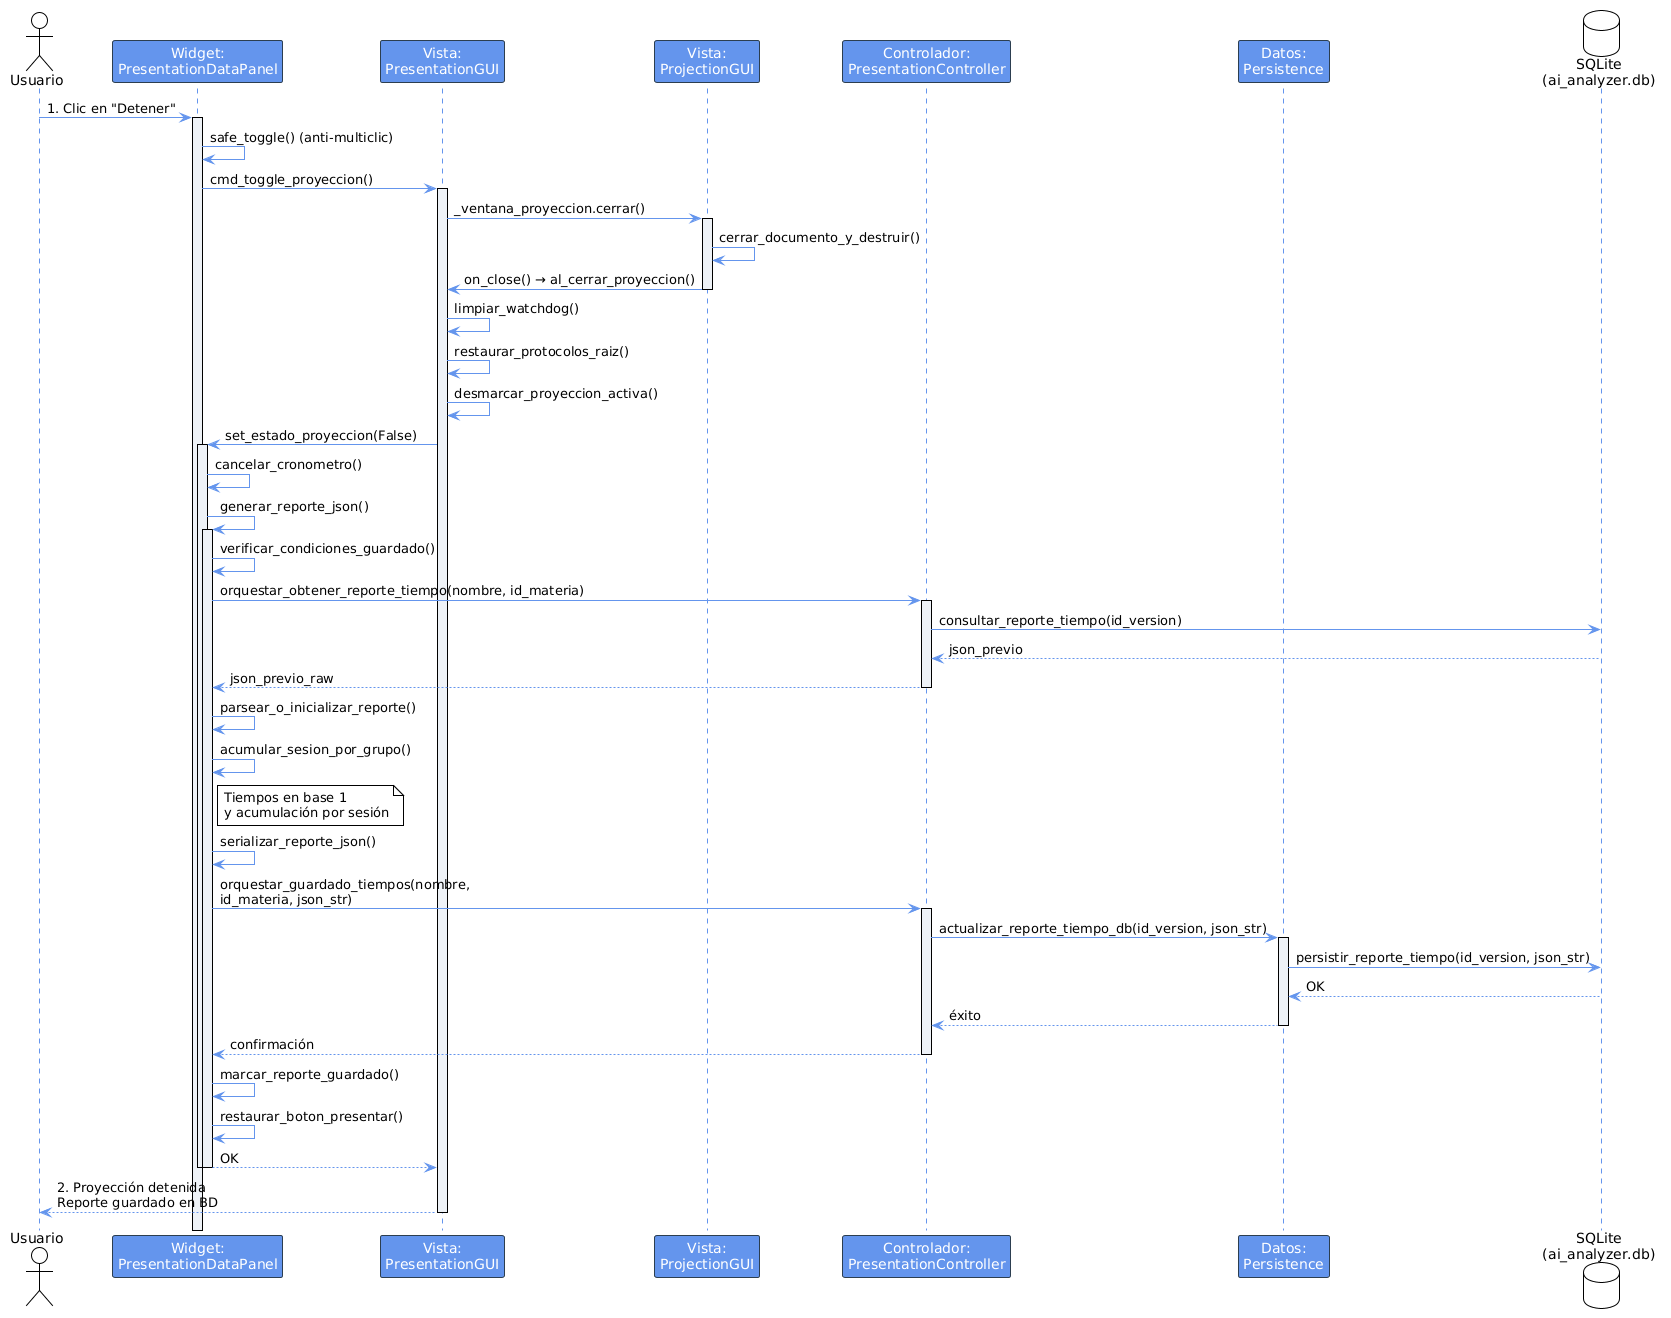
\includegraphics[width=0.95\textwidth]{TT-II/Fig26.png}
    \caption{Diagrama de secuencia de la detención de la exposición y la persistencia de tiempos.}
    \label{fig:secuencia-prototipo-2-detencion-persistencia}
\end{figure}

\begin{figure}[!htbp]
    \centering
    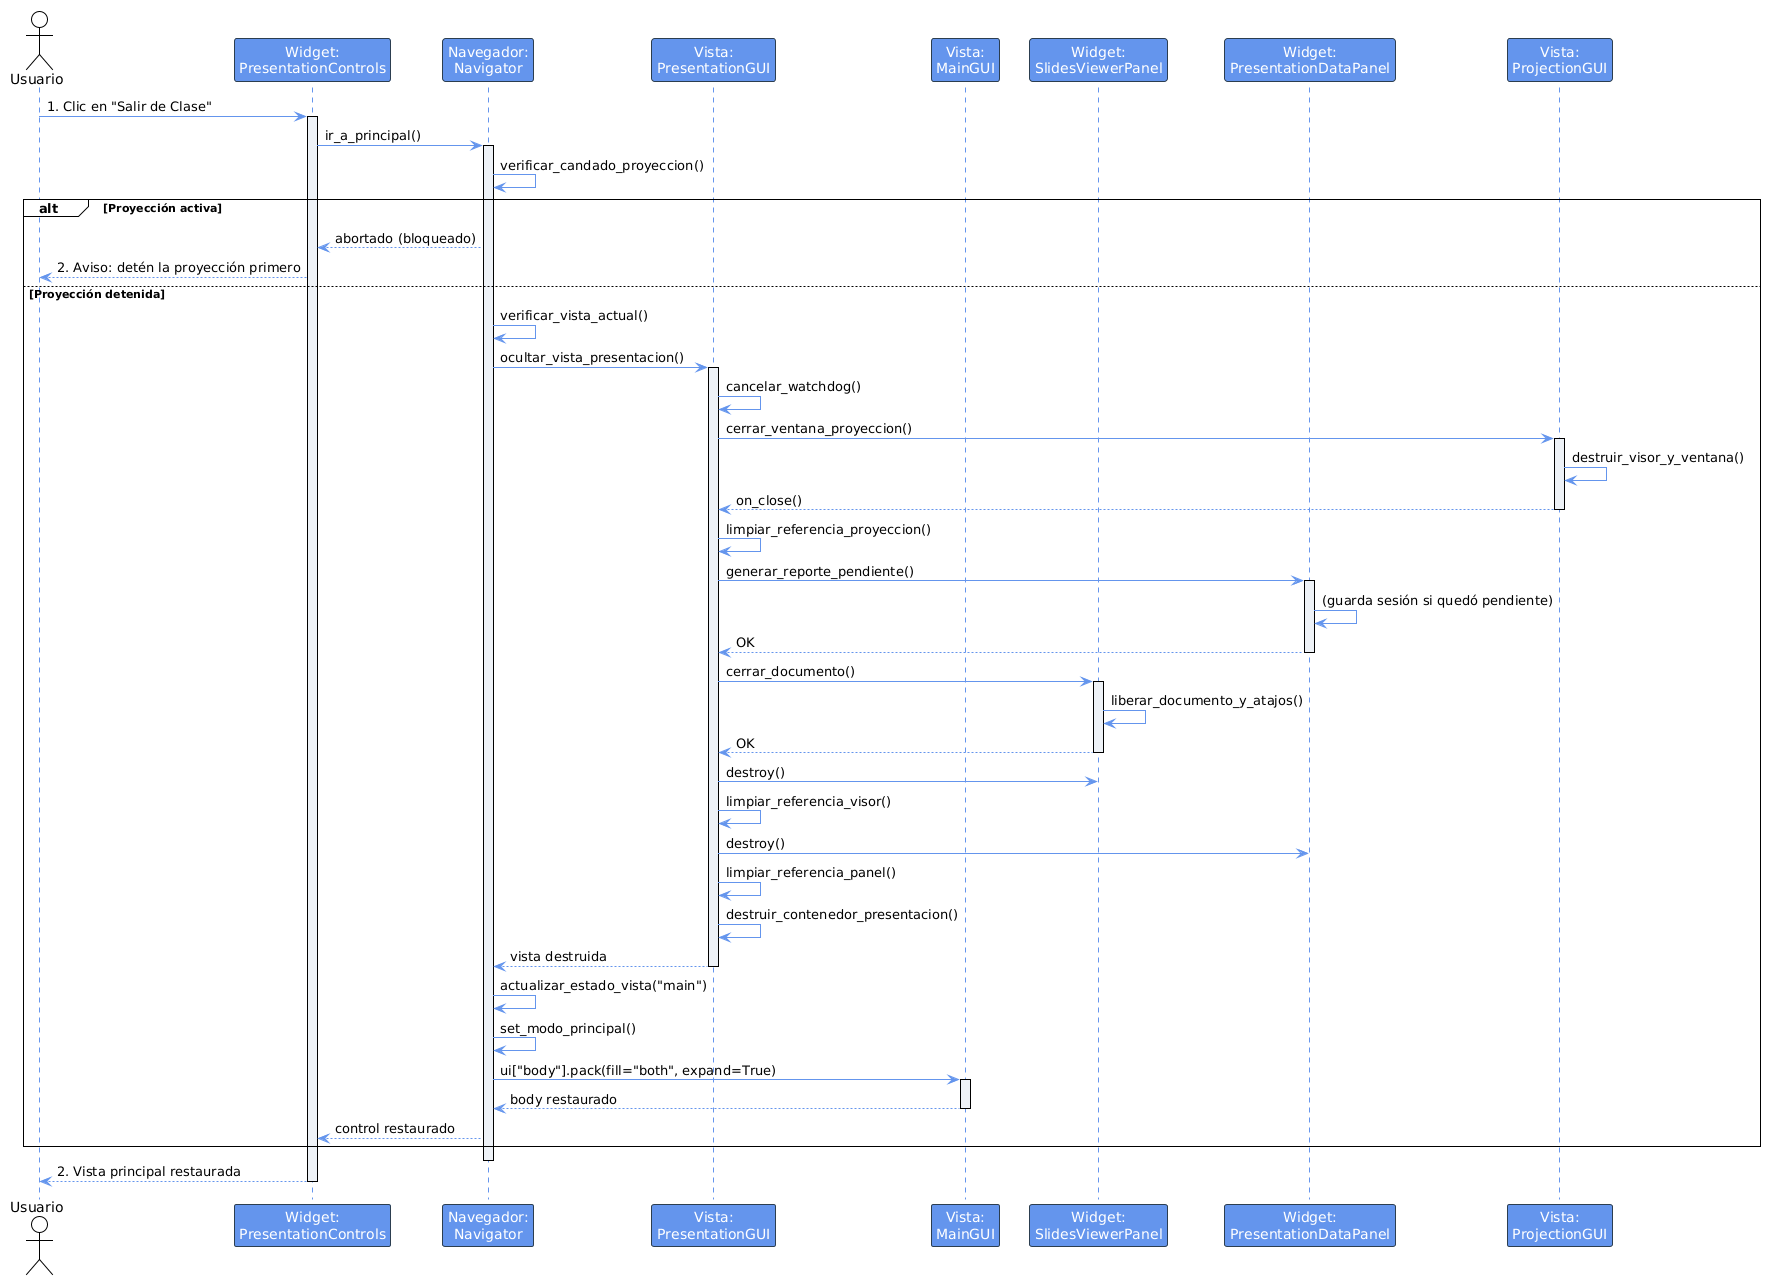
\includegraphics[width=0.95\textwidth]{TT-II/Fig27.png}
    \caption{Diagrama de secuencia de la salida de la vista y la restauración del estado anterior.}
    \label{fig:secuencia-prototipo-2-salida-restauracion}
\end{figure}

\clearpage
\subsubsection*{Protocolo de Pruebas del Prototipo 2}
\addcontentsline{toc}{subsubsection}{\protect\ttiiTOC{Protocolo de Pruebas del Prototipo 2}}

Para el prototipo 2, orientado al modo de presentación en vivo y la proyección en una pantalla secundaria, se mantuvo la nomenclatura compuesta por un prefijo de tres letras y un número consecutivo establecida en el prototipo 1. El prefijo identifica el módulo o la categoría evaluada y el número distingue cada caso de prueba dentro de ella. La Tabla \ref{tab:nomenclatura-pruebas-prototipo-2} presenta el significado de las siglas empleadas.

\begin{table}[H]
    \centering
    \renewcommand{\arraystretch}{1.2}
    \ttstyle
    \begin{tabularx}{\textwidth}{>{\centering\arraybackslash}p{1.5cm}p{4.6cm}X}
        \toprule
        \textbf{Sigla} & \textbf{Módulo o categoría} & \textbf{Significado dentro del protocolo} \\
        \midrule
        PMD & Modo de presentación & Pruebas del Modo de Presentación en Vivo, destinadas a validar el acceso desde la tarjeta, el ensamblaje de la vista, la configuración de la sesión, los controles de navegación y los cronómetros. \\
        \hairrule
        PRY & Proyección & Pruebas de Proyección, orientadas a verificar la ventana secundaria, el bloqueo de acciones de cierre y la detección de desconexiones del dispositivo de salida. \\
        \hairrule
        SNC & Sincronización & Pruebas de Sincronización, utilizadas para comprobar la propagación de los cambios de diapositiva entre el visor, el panel de datos y la proyección. \\
        \hairrule
        PRD & Persistencia del reporte & Pruebas del Reporte de Tiempos, destinadas a validar la generación del JSON, el almacenamiento incremental por grupo y la reanudación de sesiones. \\
        \hairrule
        STR & Pruebas de estrés & Pruebas de Estrés, que agrupan escenarios de interacción repetida, cierres forzados, navegación intensiva y desconexiones abruptas. \\
        \hairrule
        INT & Integridad & Pruebas de Integridad, destinadas a verificar la consistencia del reporte de tiempos, los índices en base uno y la estructura acumulativa por grupo. \\
        \hairrule
        USR & Pruebas de usuario & Pruebas de Usuario, que agrupan escenarios derivados de la interacción directa con el modo de presentación y sus formularios. \\
        \bottomrule
    \end{tabularx}
    \caption{Nomenclatura de los identificadores de las pruebas del prototipo 2.}
    \label{tab:nomenclatura-pruebas-prototipo-2}
\end{table}

\textbf{Módulo: Modo de Presentación en Vivo}

\textbf{Objetivo:} Validar el funcionamiento del modo de presentación en vivo, asegurando que el prototipo pueda ensamblar el entorno de exposición, desplegar y validar el formulario de configuración de la sesión, controlar la navegación entre diapositivas, registrar los tiempos de exposición y detener la sesión de forma segura.

\textbf{Descripción del flujo:}
\begin{enumerate}
    \item Acceder al modo de presentación desde la tarjeta de una presentación, abriendo el menú ``Opciones'' y seleccionando ``Presentar clase''. La versión debe estar analizada previamente; de lo contrario se muestra el aviso ``Análisis requerido''.
    \item Ensamblar el visor de diapositivas y el panel de datos generado por la IA.
    \item Cargar en memoria las notas, preguntas y datos de interés asociados a cada diapositiva.
    \item Desplegar el formulario modal con los campos de grupo, tiempo estimado y dispositivo de salida al pulsar ``Presentar'' en el panel.
    \item Validar el grupo, el intervalo de tiempo permitido y la selección del dispositivo de salida.
    \item Reanudar la sesión desde la última diapositiva registrada para el grupo seleccionado.
    \item Iniciar el cronómetro total y el cronómetro individual por diapositiva al confirmar el formulario.
    \item Navegar mediante los controles de la interfaz, los atajos de teclado y el salto directo por índice.
    \item Detener la sesión con ``Detener'' o abandonar la vista, y generar el reporte de tiempos correspondiente.
\end{enumerate}

\textbf{Arquitectura del módulo:}
\begin{verbatim}
Módulo de Presentación en Vivo
|-- Frontend (Capa de Presentación)
|   |-- views/
|   |   |-- presentation_gui.py
|   |   |-- navigator.py
|   |   `-- ui_state.py
|   `-- widgets/presentation_mode/
|       |-- presentation_controls.py
|       |-- presentation_data_panel.py
|       `-- slides_viewer_panel.py
|-- Core (Capa de Controladores y Lógica de Negocio)
|   |-- controller/
|   |   |-- presentation_controller.py
|   |   `-- subject_controller.py
|   `-- logic/
|       `-- slide_processor.py
|-- Infrastructure
|   `-- utils/thread_manager.py
`-- Data (Capa de Acceso a Datos)
    |-- persistence.py
    |-- queries.py
    `-- database_manager.py
\end{verbatim}

\textbf{Componentes que probar:}

\begin{table}[H]
    \centering
    \ttstyle
    \begin{tabular}{L{0.34\textwidth}L{0.18\textwidth}L{0.38\textwidth}}
        \toprule
        \textbf{Componente} & \textbf{Tipo} & \textbf{Descripción} \\
        \midrule
        Vista principal (\texttt{presentation\_gui.py}) & UI/Frontend & Ensambla el contenedor, incorpora el visor y el panel de datos, y gestiona el formulario modal de configuración. \\
        \hairrule
        Panel de datos (\texttt{presentation\_data\_panel.py}) & UI/Frontend & Muestra los cronómetros, los controles de navegación y sesión, y las notas generadas por la IA. \\
        \hairrule
        Visor (\texttt{slides\_viewer\_panel.py}) & UI/Frontend & Renderiza el PDF y emite los eventos asociados con los cambios de diapositiva. \\
        \hairrule
        Controles (\texttt{presentation\_controls.py}) & UI/Frontend & Widget legado de navegación. En la versión actual no se instancia: los controles (anterior, siguiente, salto por índice y Presentar/Detener) se construyen dentro de \texttt{presentation\_data\_panel.py}. \\
        \hairrule
        Orquestador (\texttt{presentation\_controller.py}) & Backend/Controller & Consulta y guarda los reportes de tiempo, recupera el análisis y coordina el inicio de la proyección. \\
        \hairrule
        Persistencia (\texttt{persistence.py}, \texttt{queries.py}) & Base de datos & Realiza la lectura y escritura del reporte de tiempos en \texttt{Historial\_de\_Versiones}. \\
        \bottomrule
    \end{tabular}
    \caption{Componentes del módulo de presentación en vivo.}
    \label{tab:componentes-modulo-presentacion}
\end{table}

\clearpage
\textbf{Cobertura de pruebas --- Presentación en vivo:}

{\ttpruebasetup
\begin{longtable}{@{}p{\linewidth}@{}}
\ttcase{PMD-01}{Ensamblaje de la vista}{Seleccionar ``Presentar clase'' desde el menú ``Opciones'' de la tarjeta, con la versión ya analizada.}{Se oculta el contenido principal y se muestran el visor y el panel de datos.}{Sí}{El menú de opciones se cierra y el contenido principal desaparece. En su lugar se monta un contenedor con el visor de diapositivas en la parte izquierda y el panel ``Apoyo de Clase'' en la parte derecha. La barra superior cambia para mostrar ``Presentando: <nombre del archivo>''. El ensamblado se completa en menos de un segundo.}
\ttcase{PMD-02}{Carga del análisis de IA}{Al ensamblar la vista, consultar el análisis de la versión activa.}{Las notas, preguntas y datos de interés quedan disponibles en memoria.}{Sí}{Al navegar entre diapositivas, el panel ``Apoyo de Clase'' muestra inmediatamente las preguntas de comprensión y los datos de interés correspondientes a cada diapositiva, confirmando que el análisis fue cargado correctamente al ensamblar la vista.}
\ttcase{PMD-03}{Apertura del formulario}{Pulsar ``Presentar'' en el panel de datos.}{Se despliega el formulario con los campos de grupo, tiempo y monitor.}{Sí}{Se abre el formulario ``Configuración de Sesión'' con tres secciones: la primera para ingresar o seleccionar el grupo escolar, la segunda para definir el tiempo estimado de la exposición con el valor 60 como predeterminado, y la tercera para seleccionar el dispositivo de salida. El formulario permanece siempre al frente y bloquea la interacción con el resto de la interfaz hasta ser cerrado.}
\ttcase{PMD-04}{Validación de grupo vacío}{Confirmar con ``Crear Nuevo'' y el campo vacío.}{Se impide continuar y se muestra un mensaje de campo obligatorio.}{Sí}{El formulario no se cierra y aparece el mensaje ``Error: El campo de grupo no puede estar vacío.'' en color rojo debajo de los campos de entrada.}
\ttcase{PMD-05}{Longitud máxima del grupo}{Ingresar ``3CM2X'' (6 caracteres).}{Se rechaza el valor y se informa el límite permitido.}{Sí}{El formulario no se cierra y aparece el mensaje ``Error: Grupo debe ser alfanumérico (máx 5 caracteres).'' en color rojo. El identificador ingresado se convierte automáticamente a mayúsculas.}
\ttcase{PMD-06}{Intervalo del tiempo estimado}{Ingresar un tiempo de 120 minutos.}{Se rechaza el valor e informa el intervalo de 1 a 90 minutos.}{Sí}{El formulario no se cierra y aparece el mensaje ``Error: El tiempo debe ser mayor a 0 y máximo 90 min.'' en color rojo. El campo de tiempo permanece editable con el valor ingresado. El valor 90 sí es aceptado por el formulario.}
\ttcase{PMD-07}{Selección del monitor principal}{Seleccionar la pantalla principal como dispositivo de salida y confirmar.}{Se impide iniciar la exposición y se solicita una pantalla secundaria.}{Sí}{Al seleccionar la pantalla principal como dispositivo de salida y confirmar la configuración, aparece un aviso que indica que no se puede iniciar la clase y que se debe conectar un proyector o un monitor secundario para comenzar. La exposición no inicia en la pantalla principal.}
\ttcase{PMD-08}{Bloqueo de clics repetidos}{Pulsar ``Presentar'' cinco veces de forma consecutiva.}{Se procesa un único inicio de sesión.}{Sí}{Al pulsar ``Presentar'' por primera vez, los botones ``Presentar'' y ``Detener'' quedan deshabilitados durante un segundo. Los clics adicionales realizados durante ese intervalo no abren formularios adicionales ni crean proyecciones duplicadas. Al concluir el segundo, los botones recuperan su estado normal.}
\ttcase{PMD-09}{Reanudación por grupo}{Elegir un grupo con última diapositiva registrada en la posición 5.}{El visor se posiciona en la diapositiva 5.}{Sí}{Al confirmar el formulario con ese grupo, el visor, el contador de página y la proyección se posicionan automáticamente en la diapositiva 5, mostrando su contenido y las anotaciones de IA correspondientes.}
\ttcase{PMD-10}{Navegación con botones}{Utilizar los botones ``Anterior'' y ``Siguiente'' del pie del panel.}{El visor cambia de diapositiva y actualiza el contador.}{Sí}{Al pulsar cualquiera de los botones, el visor renderiza la diapositiva correspondiente, el campo de número de página se actualiza y el panel ``Apoyo de Clase'' muestra las anotaciones de esa diapositiva. Después de cada pulsación, los botones quedan deshabilitados durante 400 milisegundos para evitar cambios involuntarios por doble clic.}
\ttcase{PMD-11}{Navegación con teclado}{Utilizar flechas, barra espaciadora, Enter, RePág y AvPág.}{El visor responde de la misma manera que con los botones.}{Sí}{Todas las teclas mencionadas producen el mismo cambio de diapositiva que los botones de navegación, incluso cuando el foco de la interfaz no está sobre el visor. El panel y la proyección se actualizan de la misma forma.}
\ttcase{PMD-12}{Salto directo por índice}{Ingresar el valor 10 en el campo de índice y presionar Enter.}{El visor muestra la diapositiva 10.}{Sí}{Al presionar Enter, el visor renderiza la diapositiva 10, el contador de página muestra ``10 / <total>'' y el panel ``Apoyo de Clase'' carga las anotaciones correspondientes a esa diapositiva.}
\ttcase{PMD-13}{Controles en los extremos}{Llegar a la primera y a la última diapositiva.}{El control que excedería el límite se deshabilita.}{Sí}{Al estar en la primera diapositiva, el botón ``Anterior'' aparece deshabilitado visualmente y no responde a clics. Al estar en la última, el botón ``Siguiente'' queda deshabilitado de la misma forma. El campo de número de página conserva el índice válido en ambos casos.}
\ttcase{PMD-14}{Cronómetro total}{Iniciar una sesión y observar el cronómetro durante 30 segundos.}{El tiempo avanza continuamente en formato minutos y segundos.}{Sí}{El cronómetro ``TOTAL (Sesión)'' avanza de forma continua segundo a segundo desde 00:00 hasta 00:30, sin saltos ni pausas, durante todo el tiempo que la sesión permaneció activa.}
\ttcase{PMD-15}{Cronómetro por diapositiva}{Cambiar de diapositiva y volver a la anterior.}{Cada diapositiva conserva su tiempo acumulado.}{Sí}{Al regresar a una diapositiva visitada anteriormente, el cronómetro ``ESTA SLIDE'' recupera el tiempo acumulado previamente para esa diapositiva y continúa sumando desde ese valor, sin reiniciarse.}
\ttcase{PMD-16}{Aviso por exceso de tiempo}{Configurar un minuto y mantener la sesión durante 90 segundos.}{El cronómetro total cambia a color rojo.}{Sí}{Al superar el tiempo estimado configurado, el cronómetro ``TOTAL (Sesión)'' cambia su color a rojo, indicando visualmente al docente que excedió el tiempo planificado. Cuando el tiempo vuelve a estar por debajo del estimado, el cronómetro recupera su color original.}
\ttcase{PMD-17}{Grupo nuevo y existente}{Alternar entre ``Seleccionar'' y ``Crear Nuevo''.}{El selector y el campo de captura se alternan correctamente.}{Sí}{Al elegir ``Seleccionar'', el formulario muestra el menú desplegable con los grupos existentes y el botón de eliminar grupo. Al elegir ``Crear Nuevo'', el desplegable desaparece y en su lugar aparece el campo de texto para ingresar el nuevo identificador. En cada alternancia solo queda visible el control correspondiente a la opción activa.}
\ttcase{PMD-18}{Detención de la sesión}{Seleccionar el botón ``Detener''.}{Se detienen los cronómetros y se genera el reporte de tiempos.}{Sí}{La ventana de proyección se cierra, los cronómetros dejan de avanzar, el reporte de tiempos de la sesión queda guardado en la base de datos y el botón cambia de ``Detener'' a ``Presentar'', indicando que el panel está listo para iniciar una nueva sesión.}
\ttcase{PMD-19}{Eliminar grupo seleccionado}{Pulsar el botón de papelera y confirmar la eliminación de un grupo con sesiones registradas.}{El grupo y su historial se eliminan; la lista se actualiza.}{Sí}{Al pulsar el botón de papelera, se muestra el cuadro de confirmación ``Eliminar grupo'' con el mensaje ``¿Deseas eliminar el grupo y su historial de sesiones?'' y los botones ``Sí'' y ``No''. Al confirmar, el grupo desaparece del menú desplegable y todos sus registros de sesión son eliminados. Si era el único grupo registrado, el formulario cambia automáticamente al modo ``Crear Nuevo'' y el botón de papelera queda deshabilitado.}
\ttcase{PMD-20}{Cancelar eliminación de grupo}{Pulsar el botón de papelera y responder ``No'' en el cuadro de confirmación.}{Se conserva el grupo y todos sus registros.}{Sí}{Al pulsar ``No'', el cuadro de confirmación se cierra sin realizar ningún cambio. El grupo permanece seleccionado en el menú desplegable y el formulario de configuración continúa abierto con el mismo estado.}
\ttcase{PMD-21}{Acceso sin análisis previo}{Seleccionar ``Presentar clase'' con una versión sin analizar.}{Se bloquea el acceso con un aviso.}{Sí}{Se muestra el modal ``Análisis requerido'' con el mensaje ``Para poder presentar la clase, primero debes ejecutar el Análisis de IA sobre esta versión.'' El contenido principal no se oculta y no se navega hacia la vista de presentación.}
\ttcase{PMD-22}{Cambio de grupo antes de iniciar}{Elegir un segundo grupo con distinta última diapositiva y confirmar.}{La sesión reanuda en la diapositiva registrada para ese grupo.}{Sí}{Al confirmar el formulario con el segundo grupo, la sesión inicia desde la diapositiva registrada para ese grupo específico. Los cronómetros comienzan desde cero para la nueva sesión, independientemente del tiempo acumulado en sesiones anteriores de ese mismo grupo.}
\ttcase{PMD-23}{Salida sin proyección}{Con la sesión detenida, usar el botón de regreso de la topbar.}{Se guarda el avance y se restaura la vista principal.}{Sí}{Al pulsar el botón de regreso, el avance de la sesión queda guardado en la base de datos, el visor y el panel de datos son destruidos y la vista principal con la cuadrícula de presentaciones vuelve a mostrarse.}
\ttcase{PMD-24}{Alternancia Presentar/Detener}{Observar el botón durante la sesión activa.}{Solo uno de los dos controles está visible.}{Sí}{Al iniciar la sesión, el botón ``Presentar'' desaparece y en su lugar aparece el botón ``Detener'' en la misma posición. Al detener la sesión, ocurre lo inverso: ``Detener'' desaparece y ``Presentar'' vuelve a mostrarse. En ningún momento ambos botones están visibles al mismo tiempo.}
\ttcaselast{PMD-25}{Cronómetro antes de iniciar}{Abrir la vista y esperar sin confirmar el formulario.}{Los cronómetros permanecen en 00:00.}{Sí}{Los cronómetros ``TOTAL (Sesión)'' y ``ESTA SLIDE'' permanecen en 00:00 mientras no se confirme el formulario de configuración de la sesión. El conteo solo inicia una vez que la proyección ha sido creada exitosamente.}
\caption{Casos de prueba del módulo de presentación en vivo.}
\label{tab:casos-prueba-modulo-presentacion}
\end{longtable}
}

\clearpage
\textbf{Módulo: Proyección en Pantalla Secundaria}

\textbf{Objetivo:} Validar el funcionamiento de la ventana de proyección, asegurando que el prototipo pueda abrir una vista sin bordes en el monitor secundario, impedir cierres accidentales, mantener la sincronización con el visor principal y detectar la desconexión del dispositivo mediante un mecanismo de vigilancia.

\textbf{Descripción del flujo:}
\begin{enumerate}
    \item Calcular las coordenadas y la resolución del monitor seleccionado en el formulario.
    \item Crear una ventana \texttt{CTkToplevel} sin bordes con la geometría del dispositivo de salida.
    \item Bloquear las acciones de cierre mediante Alt+F4, Escape y el protocolo de cierre de la ventana.
    \item Instanciar un visor secundario que muestre la diapositiva activa.
    \item Registrar los monitores conectados al iniciar la proyección y comprobar cada 2 segundos que se mantengan la cantidad y la geometría del dispositivo de salida.
    \item Cerrar la proyección de manera controlada y avisar al docente si dos lecturas consecutivas detectan que el dispositivo de salida dejó de estar disponible.
\end{enumerate}

\textbf{Arquitectura del módulo:}
\begin{verbatim}
Módulo de Proyección
|-- Frontend
|   |-- views/
|   |   |-- presentation_gui.py
|   |   `-- projection_gui.py
|   `-- widgets/presentation_mode/
|       `-- slides_viewer_panel.py
|-- Infrastructure
|   `-- screeninfo
`-- Core
    `-- controller/presentation_controller.py
\end{verbatim}

\clearpage
\textbf{Componentes que probar:}

\begin{table}[H]
    \centering
    \ttstyle
    \begin{tabular}{L{0.34\textwidth}L{0.18\textwidth}L{0.38\textwidth}}
        \toprule
        \textbf{Componente} & \textbf{Tipo} & \textbf{Descripción} \\
        \midrule
        Ventana de proyección (\texttt{projection\_gui.py}) & UI/Frontend & Crea la ventana secundaria sin bordes, incorpora el visor y controla su cierre. \\
        \hairrule
        Detección de monitores (\texttt{screeninfo}) & Infraestructura & Obtiene las coordenadas, la resolución y la disponibilidad de los monitores conectados. \\
        \hairrule
        Mecanismo de vigilancia (\texttt{presentation\_gui.py}) & Lógica & Registra los monitores al iniciar la proyección y comprueba cada 2 s que se mantengan la cantidad y geometría; tras dos lecturas consecutivas de desconexión, cierra la proyección y avisa al docente. \\
        \hairrule
        Bloqueos de teclado (\texttt{projection\_gui.py}) & Lógica & Impide el cierre accidental mediante Alt+F4, Escape y \texttt{WM\_DELETE\_WINDOW}. \\
        \bottomrule
    \end{tabular}
    \caption{Componentes del módulo de proyección.}
    \label{tab:componentes-modulo-proyeccion}
\end{table}

\textbf{Cobertura de pruebas --- Proyección:}

{\ttpruebasetup
\begin{longtable}{@{}p{\linewidth}@{}}
\ttcase{PRY-01}{Ausencia de monitor secundario}{Intentar presentar con un solo monitor conectado.}{Se muestra una advertencia y no se inicia la proyección.}{Sí}{La validación del dispositivo de salida está habilitada: al pulsar el botón de presentación, el prototipo enumera los monitores conectados y, al detectar una sola pantalla, muestra el aviso ``Proyector no detectado'', indicando que se debe conectar un proyector o monitor secundario, sin abrir el formulario de configuración. Además, el selector de dispositivo de salida del formulario únicamente acepta la opción ``[Proyector/Ext]'', por lo que no es posible iniciar la sesión con la pantalla principal o la pantalla simulada.}
\ttcase{PRY-02}{Apertura de la proyección}{Confirmar el formulario con un monitor secundario conectado.}{La ventana se abre sin bordes en el monitor secundario.}{Sí}{La ventana de proyección se abre en el monitor secundario seleccionado, ocupando su resolución completa y sin mostrar ningún marco, barra de título ni controles de ventana. La diapositiva activa se presenta sobre un fondo negro.}
\ttcase{PRY-03}{Bloqueo de Escape}{Presionar Escape en la ventana de proyección.}{El evento se ignora y la proyección permanece activa.}{Sí}{Al presionar Escape en la ventana de proyección, la ventana no se cierra ni cambia de estado. La diapositiva activa permanece visible sin ninguna alteración.}
\ttcase{PRY-04}{Bloqueo de Alt+F4}{Presionar Alt+F4 en la proyección.}{La solicitud de cierre se bloquea.}{Sí}{Al presionar Alt+F4 sobre la ventana de proyección, la solicitud de cierre es ignorada y la ventana permanece abierta mostrando la diapositiva activa. La proyección solo puede cerrarse desde el botón ``Detener'' del panel del docente.}
\ttcase{PRY-05}{Bloqueo en la ventana principal}{Presionar Escape en la ventana principal durante la proyección.}{El evento se ignora mientras la sesión está activa.}{Sí}{Durante una proyección activa, presionar Escape en la ventana principal del docente no produce ninguna acción visible. Al detener la sesión, el atajo recupera su comportamiento normal.}
\ttcase{PRY-06}{Cierre desde los controles}{Seleccionar ``Detener'' desde el panel de control.}{La proyección se cierra y libera sus recursos.}{Sí}{La ventana de proyección se cierra, los cronómetros se detienen, el reporte de tiempos se guarda y el botón del panel del docente cambia de ``Detener'' a ``Presentar''.}
\ttcase{PRY-07}{Sincronización inicial}{Abrir la proyección con el visor en la diapositiva 7.}{La proyección y la vista del docente se posicionan en la última diapositiva registrada para el grupo seleccionado; con un grupo nuevo, ambas inician en la diapositiva 1.}{Sí}{La proyección no toma la diapositiva activa en el visor al momento de iniciarse: tanto la vista del docente como la proyección se reposicionan en la última diapositiva registrada para el grupo seleccionado en el historial de sesiones, lo que permite reanudar la exposición donde concluyó la sesión anterior. Con un grupo nuevo, ambas vistas inician en la diapositiva 1, independientemente de la diapositiva que estuviera mostrando el visor del docente.}
\ttcase{PRY-08}{Detección de desconexión}{Desconectar el monitor secundario durante la sesión.}{La proyección se cierra y se muestra una advertencia.}{Sí}{El mecanismo de vigilancia está habilitado: al iniciar la proyección se registran los monitores conectados (cantidad de pantallas y geometría del monitor de salida) y una rutina verifica cada 2 s que persistan, reaccionando sin importar la posición del proyector (izquierda, derecha o arriba). Para descartar falsas enumeraciones, exige dos lecturas consecutivas; por ello, la proyección se cierra aproximadamente 4 s después de la desconexión real. La ventana se destruye, el panel del docente vuelve a mostrar el botón ``Presentar'', Escape se desbloquea en la ventana principal y aparece el aviso ``Conexión Perdida'', que indica que la presentación se detuvo por seguridad.}
\ttcase{PRY-09}{Reconexión del dispositivo}{Reconectar rápidamente el monitor secundario.}{El prototipo mantiene un estado consistente y permite reiniciar la proyección.}{Sí}{Si la reconexión ocurre antes de que el mecanismo de vigilancia acumule dos lecturas consecutivas de desconexión, la sesión continúa sin interrupción. Si la desconexión persiste, la proyección se cierra con el aviso correspondiente y el estado queda consistente (botón ``Presentar'' activo y Escape desbloqueado). Al reconectar el monitor, el docente puede reiniciar la proyección desde el panel; antes de abrir el formulario de configuración, se vuelve a validar la disponibilidad de los monitores.}
\ttcase{PRY-10}{Resolución del monitor}{Proyectar en un monitor de 1920$\times$1080 píxeles.}{La ventana ocupa exactamente la resolución seleccionada.}{Sí}{Se comprobó que la ventana de proyección se muestra correctamente con la resolución seleccionada de 1920$\times$1080 píxeles y ocupa el área correspondiente del monitor, sin recortes ni desajustes visibles.}
\ttcase{PRY-11}{Bloqueo de salida al menú}{Usar el botón de regreso de la topbar durante una proyección activa.}{La navegación se bloquea y se solicita detener primero la sesión.}{Sí}{Al pulsar el botón de regreso de la barra superior durante una proyección activa, la navegación hacia el menú principal es bloqueada y no se produce ningún cambio de vista. El docente debe detener la sesión primero para poder regresar al panel principal. El bloqueo no muestra un modal al usuario; opera de forma silenciosa.}
\ttcase{PRY-12}{Grupo nuevo en la proyección}{Confirmar el formulario con un grupo sin sesiones previas.}{La proyección inicia en la diapositiva 1.}{Sí}{Al seleccionar un grupo que no tiene sesiones previas registradas, la ventana de proyección se abre mostrando la primera diapositiva de la presentación, tanto en la vista del docente como en la pantalla de proyección.}
\ttcase{PRY-13}{Restauración tras detener}{Pulsar ``Detener'' y observar el panel.}{La proyección se cierra y vuelve el botón ``Presentar''.}{Sí}{La ventana de proyección se cierra, los cronómetros dejan de avanzar, el reporte de tiempos queda guardado y el panel del docente regresa a su estado inicial mostrando el botón ``Presentar'' en lugar de ``Detener''.}
\ttcase{PRY-14}{Fondo de la proyección}{Observar la ventana durante la exposición.}{Se muestra la diapositiva sobre fondo negro y sin bordes.}{Sí}{La ventana de proyección muestra la diapositiva activa sobre un fondo completamente negro, sin marcos, sin barra de título y sin ningún control visible. La imagen de la diapositiva se ajusta al tamaño disponible de la ventana.}
\ttcaselast{PRY-15}{Cierre al abandonar la vista}{Regresar al menú con la sesión detenida.}{La proyección se cierra y se liberan los recursos.}{Sí}{Al pulsar el botón de regreso con la sesión detenida, la ventana de proyección se cierra antes de que el visor y el panel sean destruidos, y la vista principal con la cuadrícula de presentaciones vuelve a mostrarse sin rastros del modo de presentación.}
\caption{Casos de prueba del módulo de proyección.}
\label{tab:casos-prueba-modulo-proyeccion}
\end{longtable}
}

\clearpage
\textbf{Módulo: Sincronización entre Visor, Panel y Proyector}

\textbf{Objetivo:} Validar que cualquier cambio de diapositiva se propague de manera consistente entre el visor principal, el panel de datos con contenido generado por la IA y la ventana de proyección.

\textbf{Descripción del flujo:}
\begin{enumerate}
    \item El usuario solicita un cambio de página mediante los botones, el teclado o el campo de salto directo.
    \item El visor actualiza \texttt{pagina\_actual} y renderiza la nueva diapositiva.
    \item Se emite el evento \texttt{on\_pagina\_cambiada} hacia los componentes suscritos.
    \item El panel de datos actualiza las notas, el contador y el cronómetro de la diapositiva.
    \item La ventana de proyección sincroniza su visor cuando se encuentra activa.
\end{enumerate}

\clearpage
\textbf{Componentes que probar:}

\begin{table}[H]
    \centering
    \ttstyle
    \begin{tabular}{L{0.34\textwidth}L{0.18\textwidth}L{0.38\textwidth}}
        \toprule
        \textbf{Componente} & \textbf{Tipo} & \textbf{Descripción} \\
        \midrule
        Visor principal (\texttt{slides\_viewer\_panel.py}) & UI/Frontend & Renderiza el PDF y emite el evento \texttt{on\_pagina\_cambiada}. \\
        \hairrule
        Panel de datos (\texttt{presentation\_data\_panel.py}) & UI/Frontend & Actualiza el contenido generado por la IA, el contador y los cronómetros. \\
        \hairrule
        Proyección (\texttt{projection\_gui.py}) & UI/Frontend & Expone \texttt{sincronizar\_pagina(numero)} para alinear el visor secundario. \\
        \hairrule
        Evento central (\texttt{presentation\_gui.py}) & Lógica & Conecta los componentes mediante el evento de cambio de página. \\
        \bottomrule
    \end{tabular}
    \caption{Componentes involucrados en la sincronización en vivo.}
    \label{tab:componentes-modulo-sincronizacion}
\end{table}

\textbf{Cobertura de pruebas --- Sincronización:}

{\ttpruebasetup
\begin{longtable}{@{}p{\linewidth}@{}}
\ttcase{SNC-01}{Visor a panel}{Avanzar una diapositiva desde el visor.}{El panel actualiza las notas y el contador.}{Sí}{Al cambiar de diapositiva en el visor, el panel ``Apoyo de Clase'' actualiza inmediatamente su contenido mostrando las preguntas de comprensión y los datos de interés correspondientes a la nueva diapositiva.}
\ttcase{SNC-02}{Visor a proyección}{Avanzar una diapositiva con la proyección activa.}{La proyección muestra la nueva diapositiva.}{Sí}{Al cambiar de diapositiva en el visor del docente, la ventana de proyección actualiza su contenido de forma inmediata mostrando la misma diapositiva que el visor principal.}
\ttcase{SNC-03}{Panel a visor}{Utilizar ``Siguiente'' desde el panel.}{El visor avanza y el contador se actualiza.}{Sí}{Al pulsar ``Siguiente'' desde el panel de datos, el visor renderiza la diapositiva siguiente y el campo de número de página se actualiza mostrando el nuevo índice.}
\ttcase{SNC-04}{Panel a proyección}{Avanzar desde el panel con la proyección activa.}{La proyección cambia de forma sincronizada.}{Sí}{Al navegar desde el panel del docente, la ventana de proyección actualiza su contenido de la misma forma que cuando el cambio se origina desde el visor, mostrando la diapositiva correspondiente sin desfase visible.}
\ttcase{SNC-05}{Salto por índice}{Ingresar el valor 15 en el campo de salto directo.}{El visor, el panel y la proyección muestran la diapositiva 15.}{Sí}{Al confirmar el salto, el visor renderiza la diapositiva 15, el campo de número de página muestra ``15 / <total>'', el panel ``Apoyo de Clase'' carga las anotaciones correspondientes y la ventana de proyección muestra esa misma diapositiva.}
\ttcase{SNC-06}{Notas por diapositiva}{Avanzar a una diapositiva con preguntas generadas por la IA.}{El panel muestra las preguntas correspondientes.}{Sí}{Al llegar a una diapositiva con contenido analizado, el panel ``Apoyo de Clase'' muestra las preguntas de comprensión y los datos de interés específicos de esa diapositiva, actualizándose automáticamente con cada cambio de página.}
\ttcase{SNC-07}{Diapositiva sin notas}{Mostrar una diapositiva sin preguntas ni datos de interés.}{Se presenta un mensaje que indica la ausencia de anotaciones.}{Sí}{El panel ``Apoyo de Clase'' muestra el texto ``Sin anotaciones de IA para esta slide.'' en lugar del contenido de preguntas y datos, indicando al docente que no hay material complementario disponible para esa diapositiva.}
\ttcase{SNC-08}{Sincronización al reanudar}{Reanudar una sesión desde la diapositiva 12.}{Todos los componentes se posicionan en la diapositiva 12.}{Sí}{Al iniciar la sesión con un grupo cuya última diapositiva registrada es la 12, el visor del docente, el contador de página, el panel ``Apoyo de Clase'' y la ventana de proyección muestran simultáneamente la diapositiva 12 desde el primer momento.}
\ttcase{SNC-09}{Reinicio de la proyección}{Cerrar y volver a abrir la proyección.}{La nueva ventana inicia en la diapositiva actual.}{Sí}{Al cerrar la proyección y volver a presentar con el mismo grupo, la nueva ventana de proyección inicia en la misma diapositiva donde terminó la sesión anterior para ese grupo, sin regresar a la primera diapositiva.}
\ttcase{SNC-10}{Cambios rápidos}{Solicitar diez cambios de diapositiva consecutivos.}{Los tres componentes permanecen sincronizados.}{Sí}{Al realizar cambios de diapositiva de forma rápida y continua, el visor, el panel y la proyección conservan la misma diapositiva activa en todo momento. No se observaron diapositivas saltadas ni desfase entre los componentes.}
\ttcase{SNC-11}{Sincronización al retroceder}{Retroceder una diapositiva desde el visor.}{El panel y la proyección retroceden junto con el visor.}{Sí}{Al retroceder desde el visor, el panel ``Apoyo de Clase'' actualiza su contenido con las anotaciones de la diapositiva anterior y la ventana de proyección muestra esa misma diapositiva, de forma simétrica al comportamiento al avanzar.}
\ttcaselast{SNC-12}{Total de diapositivas}{Abrir la vista y observar el contador.}{El panel muestra el total real de páginas del PDF.}{Sí}{El contador en el panel del docente muestra el formato ``1 / <total>'', donde el total corresponde al número real de páginas del archivo PDF de la presentación cargada.}
\caption{Casos de prueba del módulo de sincronización.}
\label{tab:casos-prueba-modulo-sincronizacion}
\end{longtable}
}

\clearpage
\textbf{Módulo: Persistencia del Reporte de Tiempos}

\textbf{Objetivo:} Validar la generación y el almacenamiento del reporte de tiempos, asegurando que el JSON producido al detener una sesión mantenga una estructura consistente, utilice índices en base uno, acumule la información por grupo y se almacene correctamente en la base de datos.

\textbf{Descripción del flujo:}
\begin{enumerate}
    \item Ejecutar \texttt{generar\_reporte\_json} al detener la sesión, al salir de la vista o al cerrar la proyección.
    \item Consultar en la base de datos el reporte previo del grupo seleccionado.
    \item Acumular los tiempos totales y los tiempos por diapositiva utilizando índices en base uno.
    \item Registrar la nueva sesión en \texttt{historial\_sesiones}.
    \item Actualizar \texttt{ultima\_diapositiva} para permitir la reanudación posterior.
    \item Enviar el JSON al controlador para su persistencia.
\end{enumerate}

\textbf{Componentes que probar:}

\begin{table}[H]
    \centering
    \ttstyle
    \begin{tabular}{L{0.34\textwidth}L{0.18\textwidth}L{0.38\textwidth}}
        \toprule
        \textbf{Componente} & \textbf{Tipo} & \textbf{Descripción} \\
        \midrule
        Generador del JSON (\texttt{presentation\_data\_panel.py}) & Lógica & Empaqueta los datos de la sesión y acumula la información registrada previamente. \\
        \hairrule
        Controlador (\texttt{presentation\_controller.py}) & Backend/Controller & Coordina el almacenamiento mediante \texttt{orquestar\_guardado\_tiempos}. \\
        \hairrule
        Persistencia (\texttt{persistence.py}) & Base de datos & Actualiza el reporte almacenado en \texttt{Historial\_de\_Versiones}. \\
        \bottomrule
    \end{tabular}
    \caption{Componentes del módulo de persistencia del reporte de tiempos.}
    \label{tab:componentes-modulo-reporte}
\end{table}

\textbf{Cobertura de pruebas --- Reporte de tiempos:}

{\ttpruebasetup
\begin{longtable}{@{}p{\linewidth}@{}}
\ttcase{PRD-01}{Generación del reporte}{Detener una sesión después de dos minutos.}{Se genera un reporte con el grupo, el tiempo total y el desglose por diapositiva.}{Sí}{Al detener la sesión, el reporte queda almacenado correctamente en la base de datos incluyendo el nombre de la presentación, el grupo, el tiempo total de la sesión, el tiempo invertido en cada diapositiva y el registro de la sesión en el historial del grupo.}
\ttcase{PRD-02}{Sesión corta}{Detener una sesión después de cinco segundos.}{El reporte se genera y almacena correctamente.}{Sí}{El reporte se genera y guarda con una duración de cinco segundos y el desglose correspondiente, sin aplicar ningún tiempo mínimo para que el guardado sea válido.}
\ttcase{PRD-03}{Sesión sin iniciar}{Solicitar la detención sin haber iniciado una exposición.}{No se genera un reporte cuando el tiempo total es cero.}{Sí}{Al intentar detener una sesión que no fue iniciada, no se escribe ningún registro en la base de datos ni se modifica ningún dato existente.}
\ttcase{PRD-04}{Acumulación por grupo}{Guardar dos sesiones correspondientes al mismo grupo.}{El tiempo total almacenado contiene la suma de ambas sesiones.}{Sí}{Al guardar la segunda sesión del mismo grupo, el tiempo total acumulado en el reporte corresponde exactamente a la suma de los tiempos de las dos sesiones, sin sobrescribir la primera.}
\ttcase{PRD-05}{Historial de sesiones}{Guardar tres sesiones para un mismo grupo.}{El historial del grupo contiene tres entradas consecutivas.}{Sí}{Cada vez que se detiene una sesión del mismo grupo, se agrega una nueva entrada numerada al historial de ese grupo. Tras tres sesiones, el historial muestra las entradas 1, 2 y 3 en orden consecutivo sin huecos.}
\ttcase{PRD-06}{Índices en base uno}{Revisar el desglose por diapositiva en el reporte.}{Las entradas comienzan en 1 y no en 0.}{Sí}{El desglose por diapositiva almacenado en el reporte usa el número de diapositiva tal como se muestra al usuario, comenzando en 1, en lugar del índice interno del visor que comienza en 0.}
\ttcase{PRD-07}{Última diapositiva}{Detener la sesión en la diapositiva 20.}{El reporte registra la diapositiva 20 como última vista.}{Sí}{El número de la última diapositiva almacenado en el reporte coincide con el número mostrado en el campo de página del panel del docente en el momento de detener la sesión.}
\ttcase{PRD-08}{Prevención de doble guardado}{Solicitar dos veces la detención de una misma sesión.}{El segundo intento no modifica el reporte ya guardado.}{Sí}{Al intentar detener la sesión por segunda vez, el reporte no se actualiza nuevamente. Los datos del primer guardado permanecen intactos en la base de datos.}
\ttcase{PRD-09}{Reanudación correcta}{Seleccionar un grupo cuya última diapositiva registrada es la quinta.}{La siguiente sesión inicia en la diapositiva 5.}{Sí}{Al iniciar una nueva sesión con ese grupo, el visor y la proyección se posicionan en la diapositiva 5 tal como se muestra al usuario, validando que el número está dentro del total de diapositivas de la presentación.}
\ttcase{PRD-10}{Persistencia en la base de datos}{Consultar el reporte guardado después de detener la sesión.}{El reporte almacenado contiene todos los datos de la sesión.}{Sí}{Al consultar el registro en la base de datos tras detener la sesión, el reporte contiene el nombre de la presentación, los datos del grupo, el tiempo total, el desglose por diapositiva y el historial de sesiones, almacenados con formato legible.}
\ttcase{PRD-11}{Formato de los tiempos}{Guardar una sesión y revisar cómo se presentan los tiempos al usuario.}{Los tiempos en el reporte se almacenan en segundos y se muestran en formato minutos:segundos solo en la interfaz.}{Sí}{El reporte almacena los tiempos como números enteros de segundos. La conversión al formato ``mm:ss'' solo ocurre al momento de mostrar los valores en los cronómetros y en el informe de rendimiento, sin modificar los datos almacenados.}
\ttcase{PRD-12}{Normalización del grupo}{Ingresar un identificador de grupo en minúsculas.}{El reporte almacena el identificador en mayúsculas.}{Sí}{Al ingresar el identificador del grupo en minúsculas, el prototipo lo convierte automáticamente a mayúsculas antes de validarlo y guardarlo. El reporte y el selector de grupos muestran siempre el identificador en mayúsculas.}
\ttcase{PRD-13}{Guardado al salir de la vista}{Abandonar el modo presentación sin pulsar ``Detener''.}{El prototipo impide abandonar la vista mientras la proyección está activa y muestra un aviso; el avance se guarda al detener la proyección con ``Detener'.}{Sí}{Al pulsar el botón ``Volver' mientras la presentación continúa proyectándose, aparece un modal con el mensaje ``No puedes regresar al menú mientras estás proyectando'. La navegación queda bloqueada y el visor y el panel permanecen abiertos. Este bloqueo corresponde al diseño del prototipo: para regresar al menú es necesario detener primero la proyección, momento en el que se guarda el avance de la sesión.}
\ttcase{PRD-14}{Cierre abrupto de la aplicación}{Cerrar la aplicación durante la sesión sin pulsar ``Detener''.}{Al cerrarse la aplicación de forma abrupta durante una sesión activa, el avance de esa sesión no se conserva; permanecen únicamente los datos de las sesiones guardadas previamente con ``Detener'.}{Sí}{No existe un mecanismo de guardado automático periódico en la versión actual del prototipo. Al cerrarse la aplicación de forma abrupta durante una sesión activa, el reporte de esa sesión no se escribe en la base de datos y el avance registrado durante la exposición no se conserva, tal como se espera en esta versión. Este comportamiento está identificado como una limitación conocida del prototipo.}
\ttcase{PRD-15}{Preservación de otros grupos}{Guardar una sesión de un grupo nuevo cuando ya existen otros.}{Los grupos previos permanecen intactos.}{Sí}{Al guardar la sesión de un nuevo grupo, el reporte de los grupos existentes no es modificado. Cada grupo conserva su propio tiempo acumulado, desglose por diapositiva y historial de sesiones de forma independiente.}
\ttcaselast{PRD-16}{Tiempo planeado en segundos}{Configurar 60 minutos y guardar la sesión.}{El reporte almacena 3600 segundos como tiempo planeado.}{Sí}{El tiempo estimado ingresado en minutos en el formulario de configuración queda convertido a segundos en el reporte, de modo que 60 minutos se almacenan como 3600 segundos para su uso en el cálculo de desviaciones del informe de rendimiento.}
\caption{Casos de prueba del módulo de persistencia del reporte de tiempos.}
\label{tab:casos-prueba-modulo-reporte}
\end{longtable}
}


\clearpage
\textbf{Módulo: Estrés, Integridad y Usuario}

\textbf{Objetivo:} Validar el comportamiento del prototipo 2 bajo condiciones de interacción intensiva y eventos inesperados, así como verificar la consistencia de los datos generados durante las sesiones de presentación.

\textbf{Descripción del flujo:} Las pruebas de este módulo exploran los siguientes escenarios específicos:
\begin{enumerate}
    \item Interacción repetida con los controles críticos de la sesión.
    \item Intentos de cierre forzado durante una proyección activa.
    \item Desconexión abrupta del dispositivo de salida.
    \item Navegación intensiva entre diapositivas.
    \item Validación de la estructura acumulativa del reporte JSON.
    \item Reanudación de sesiones a partir de información almacenada previamente.
\end{enumerate}

\textbf{Componentes que probar:}

\begin{table}[H]
    \centering
    \ttstyle
    \begin{tabular}{L{0.34\textwidth}L{0.18\textwidth}L{0.38\textwidth}}
        \toprule
        \textbf{Componente} & \textbf{Tipo} & \textbf{Descripción} \\
        \midrule
        Bloqueo de interacciones repetidas (\texttt{presentation\_data\_panel.py}) & UI/Frontend & Impide que los controles para presentar y detener procesen varias solicitudes consecutivas. \\
        \hairrule
        Mecanismo de vigilancia (\texttt{presentation\_gui.py}) & Infraestructura & Comprueba cada 2 s la cantidad y geometría de los monitores; tras dos lecturas consecutivas de desconexión, cierra la proyección y notifica al docente. \\
        \hairrule
        Generador del JSON (\texttt{presentation\_data\_panel.py}) & Lógica & Mantiene la estructura acumulativa del reporte por grupo y sesión. \\
        \hairrule
        Persistencia (\texttt{persistence.py}) & Datos & Almacena y recupera de forma íntegra el contenido de \texttt{reporte\_tiempo}. \\
        \bottomrule
    \end{tabular}
    \caption{Componentes involucrados en las pruebas de estrés, integridad y usuario del prototipo 2.}
    \label{tab:componentes-estres-prototipo-2}
\end{table}

\textbf{Cobertura de pruebas --- Estrés, integridad y usuario:}

{\ttpruebasetup
\begin{longtable}{@{}p{\linewidth}@{}}
\ttcase{STR-01}{Clics repetidos en Presentar}{Realizar diez clics en menos de un segundo.}{Se procesa una única solicitud.}{Sí}{Al pulsar ``Presentar'' repetidamente, el botón queda deshabilitado desde el primer clic durante un segundo, descartando todos los clics adicionales. Solo se abre un formulario de configuración y no se crea más de una ventana de proyección.}
\ttcase{STR-02}{Clics repetidos en Detener}{Realizar diez clics consecutivos en ``Detener''.}{Se procesa una única solicitud.}{Sí}{Al pulsar ``Detener'' repetidamente, el mecanismo de bloqueo descarta los clics adicionales. La proyección se cierra una sola vez y el reporte de tiempos se guarda una única vez sin duplicar registros.}
\ttcase{STR-03}{Cierre forzado con proyección}{Utilizar Alt+F4 durante una proyección activa.}{La solicitud de cierre se bloquea.}{Sí}{Al presionar Alt+F4 sobre la ventana de proyección durante una sesión activa, la ventana no se cierra. La diapositiva activa permanece visible y la sesión continúa sin interrupción.}
\ttcase{STR-04}{Desconexión del proyector}{Desconectar el dispositivo de salida durante la exposición.}{El prototipo detecta la desconexión mediante dos lecturas consecutivas de verificación (una cada 2 s) y detiene la proyección en aproximadamente 4 s, mostrando el aviso ``Conexión Perdida'.}{Sí}{El mecanismo de vigilancia está habilitado y revisa la disponibilidad del monitor cada 2 s. Para descartar falsas enumeraciones, requiere dos lecturas consecutivas de desconexión; por ello, la proyección se cierra aproximadamente 4 s después de la desconexión real, tiempo acorde con el diseño del mecanismo. Al cerrarse, se muestra el aviso ``Conexión Perdida'.}
\ttcase{STR-05}{Navegación intensiva}{Realizar 30 cambios de diapositiva en diez segundos.}{No se presentan errores ni pérdida de sincronización.}{Sí}{Tras 30 cambios de diapositiva realizados de forma rápida y continua, el visor, el panel ``Apoyo de Clase'' y la ventana de proyección mostraron la misma diapositiva en todo momento, sin errores de renderizado ni desincronización entre los componentes.}
\ttcase{INT-01}{Estructura del reporte}{Inspeccionar el reporte después de una sesión.}{El reporte contiene los datos del nombre del archivo, los grupos y el historial de sesiones.}{Sí}{Al consultar el reporte guardado en la base de datos, se verificó que contiene el nombre de la presentación, un bloque por cada grupo con su tiempo total, el desglose por diapositiva numerado desde 1 y el historial de sesiones con sus respectivos tiempos y fechas.}
\ttcase{INT-02}{Consistencia de los índices}{Comparar los números de diapositiva del reporte con las diapositivas de la presentación.}{El número 1 del reporte corresponde a la primera diapositiva.}{Sí}{Se verificó con una presentación de 25 diapositivas que la primera entrada del desglose corresponde a la diapositiva 1 y la última corresponde a la diapositiva 25, coincidiendo con la numeración visible al usuario en el campo de página.}
\ttcase{INT-03}{Acumulación sin duplicados}{Guardar tres sesiones para el mismo grupo.}{El tiempo total equivale a la suma exacta de las tres sesiones.}{Sí}{Tras tres sesiones del mismo grupo, el tiempo total almacenado en el reporte corresponde a la suma exacta de los tiempos de las tres sesiones, sin contabilizar ninguna sesión más de una vez.}
\ttcase{INT-04}{Persistencia entre ejecuciones}{Cerrar y volver a abrir la aplicación después de guardar una sesión.}{El reporte se recupera íntegramente.}{Sí}{Al reabrir el prototipo y consultar el reporte de tiempos guardado, todos los datos de la sesión están disponibles: grupo, tiempos por diapositiva, historial de sesiones y última diapositiva registrada.}
\ttcase{INT-05}{Reporte inválido en la base de datos}{Almacenar deliberadamente un reporte con formato inválido y presentar.}{El prototipo controla el error y genera una estructura nueva.}{Sí}{Al intentar leer un reporte con formato inválido, el prototipo no muestra ningún error al usuario. En su lugar, genera automáticamente una estructura de reporte vacía y la utiliza como punto de partida para la nueva sesión, sobrescribiendo el contenido inválido al guardar.}
\ttcase{INT-06}{Nombre del archivo en el reporte}{Revisar el campo de nombre en el reporte guardado.}{Contiene el nombre de la presentación expuesta.}{Sí}{El campo de nombre en el reporte almacenado coincide exactamente con el nombre del archivo de la presentación tal como aparece en la tarjeta de la cuadrícula principal.}
\ttcase{INT-07}{Consecutividad del historial}{Guardar sesiones con huecos en la numeración previa.}{Las entradas del historial son consecutivas desde 1.}{Sí}{Las entradas del historial de sesiones están numeradas consecutivamente a partir de 1, calculadas en función del número de sesiones existentes y no del número más alto registrado, por lo que no se generan huecos en la numeración independientemente del estado previo del reporte.}
\ttcase{USR-01}{Cancelación del formulario}{Cerrar el formulario sin confirmar la configuración.}{La proyección no se inicia.}{Sí}{Al cerrar el formulario sin pulsar ``Confirmar'', la ventana se cierra sin iniciar ninguna proyección. El panel del docente permanece en su estado anterior mostrando el botón ``Presentar''.}
\ttcase{USR-02}{Grupo con símbolos}{Ingresar un grupo que contenga un guion.}{El valor se rechaza por no ser alfanumérico.}{Sí}{Al intentar confirmar el formulario con un identificador de grupo que contiene un guion u otro símbolo no alfanumérico, el formulario no se cierra y muestra el mensaje ``Error: Grupo debe ser alfanumérico (máx 5 caracteres).'' en color rojo.}
\ttcase{USR-03}{Cierre mediante el botón de ventana}{Seleccionar el control de cierre del formulario.}{El formulario se cierra sin iniciar la sesión.}{Sí}{Al pulsar el botón de cierre de la ventana del formulario, este se cierra sin iniciar ninguna proyección. El panel del docente permanece en su estado anterior y el botón ``Presentar'' sigue visible.}
\ttcase{USR-04}{Tiempo no numérico}{Ingresar texto en el campo de tiempo estimado.}{Se solicita un número entero válido.}{Sí}{Al intentar confirmar el formulario con texto en el campo de tiempo, el formulario no se cierra y muestra el mensaje ``Error: Ingresa un número entero válido para el tiempo.'' en color rojo debajo del campo correspondiente.}
\ttcase{USR-05}{Selección del monitor principal}{Seleccionar la pantalla principal como dispositivo de salida.}{La configuración se rechaza antes de crear la proyección.}{Sí}{Al seleccionar la pantalla principal como dispositivo de salida e intentar confirmar el formulario, la proyección no inicia y se muestra en el mismo modal un mensaje de error que indica que debe elegirse un dispositivo de salida distinto de la pantalla principal.}
\ttcase{USR-06}{Índice fuera del intervalo}{Ingresar el valor 999 en el campo de salto directo.}{El campo recupera el índice de la diapositiva actual.}{Sí}{Al ingresar un número mayor al total de diapositivas de la presentación en el campo de salto directo y confirmar, el visor permanece en la diapositiva actual y el campo de número de página recupera el índice válido correspondiente, sin cambiar de diapositiva ni mostrar un error en pantalla.}
\ttcaselast{USR-07}{Cancelar el formulario con Escape}{Presionar Escape en el modal de configuración.}{El modal de configuración permanece abierto al presionar Escape, ya que esta tecla está reservada por el prototipo; el formulario se cierra únicamente con el control de cierre de la ventana.}{Sí}{Al presionar Escape en el modal de configuración, este no se cierra y el proceso no se cancela. Esto se debe a la función asignada a la tecla Escape dentro del prototipo, que no permite detener ningún proceso; el formulario se cierra únicamente mediante el control de cierre de la ventana (véase USR-03).}
\caption{Cobertura de pruebas de estrés, integridad y usuario del prototipo 2.}
\label{tab:cobertura-estres-prototipo-2}
\end{longtable}
}

\clearpage
\subsection*{Prototipo 3: Análisis de rendimiento}
\addcontentsline{toc}{subsection}{\protect\ttiiTOC{Prototipo 3: Análisis de rendimiento}}

\textbf{Introducción}

El prototipo 3 cierra el ciclo de uso del proyecto incorporando el módulo de análisis de rendimiento expositivo, que consolida y presenta de forma visual los datos registrados durante las sesiones de exposición del prototipo 2. A diferencia de los prototipos anteriores, cuyas interfaces están orientadas a la acción —cargar, analizar, exponer—, este prototipo opera de forma completamente asíncrona sobre datos ya almacenados, produciendo un informe retrospectivo que el docente puede consultar para identificar desviaciones en su ritmo de exposición y orientar la mejora de sus sesiones futuras. Este prototipo no requiere comunicación con servicios externos, ya que toda la información que procesa fue generada y persistida por los módulos anteriores.

\textbf{Objetivo}

Implementar el módulo de análisis de rendimiento que permita al docente consultar, una vez concluida una sesión de exposición, un informe detallado que contraste el tiempo real invertido en cada diapositiva con el tiempo recomendado por la IA y el tiempo estimado por el propio docente al inicio de la sesión. El informe presentará los indicadores globales de la sesión —incluyendo la etiqueta de desempeño de la presentación, las tres referencias temporales y la desviación porcentual global—, una gráfica de tendencia de tiempo por diapositiva filtrable por grupo, y un panel de desviaciones que identifique las diapositivas con mayor alejamiento respecto al tiempo recomendado, diferenciando las que duraron significativamente menos de las que duraron significativamente más.

\subsubsection*{Especificaciones (Historias de Usuario) del Prototipo 3}
\addcontentsline{toc}{subsubsection}{\protect\ttiiTOC{Especificaciones (Historias de Usuario) del Prototipo 3}}

\begin{table}[H]
    \centering
    \renewcommand{\arraystretch}{1.2}
    \ttstyle
    \begin{tabular}{p{2.5cm}p{11cm}}
        \toprule
        \textbf{ID} & \textbf{Historia de Usuario --- Acceder al informe de rendimiento} \\
        \midrule
        HU-21 & Como docente, quiero acceder al informe de rendimiento de una presentación que ya expuse, para revisar cómo fue mi desempeño durante la sesión. \\
        \hairrule
        \textbf{Prioridad} & \textbf{Criterios de aceptación} \\
        \hairrule
        Alta & El prototipo habilitará el acceso al informe de rendimiento únicamente para presentaciones que cuenten con al menos una sesión de exposición registrada con algún grupo. Las presentaciones que no hayan sido expuestas previamente no mostrarán la opción de acceder al informe.

        El prototipo mostrará en la parte superior del informe cinco indicadores globales de la sesión: la etiqueta de desempeño de la presentación (Excelente, Bueno, Regular o Deficiente), derivada de la calificación del análisis conforme a la clasificación cualitativa presentada en el marco teórico (Tabla \ref{tab:clasificacion-cualitativa-metricas}), el tiempo recomendado por la IA para la exposición completa, el tiempo estimado ingresado por el docente en el formulario de configuración, la duración real registrada por el prototipo durante la sesión y la desviación porcentual entre el tiempo real y el tiempo estimado por el docente. \\
        \bottomrule
    \end{tabular}
    \caption{Historia de Usuario --- Acceder al informe de rendimiento}
    \label{tab:hu-acceder-informe-rendimiento}
\end{table}

\begin{table}[H]
    \centering
    \renewcommand{\arraystretch}{1.2}
    \ttstyle
    \begin{tabular}{p{2.5cm}p{11cm}}
        \toprule
        \textbf{ID} & \textbf{Historia de Usuario --- Consultar tendencia de tiempo por diapositiva} \\
        \midrule
        HU-22 & Como docente, quiero visualizar una gráfica comparativa del tiempo real y el tiempo recomendado por la IA para cada diapositiva, para identificar en qué partes de mi presentación me desvié del ritmo recomendado. \\
        \hairrule
        \textbf{Prioridad} & \textbf{Criterios de aceptación} \\
        \hairrule
        Alta & El prototipo mostrará una gráfica de líneas que represente, para cada diapositiva de la presentación, el tiempo real invertido durante la exposición y el tiempo recomendado por la IA. Cada serie estará diferenciada visualmente mediante color e indicador propio. El docente podrá pasar el cursor sobre cualquier punto de la gráfica para ver el detalle de esa diapositiva.

        La gráfica podrá filtrarse por grupo mediante los selectores disponibles en la interfaz, de modo que el docente pueda comparar el comportamiento de la misma presentación en diferentes grupos. La gráfica mostrará en el eje horizontal el número de diapositiva y en el eje vertical el tiempo en segundos. \\
        \bottomrule
    \end{tabular}
    \caption{Historia de Usuario --- Consultar tendencia de tiempo por diapositiva}
    \label{tab:hu-consultar-tendencia-tiempo}
\end{table}

\begin{table}[H]
    \centering
    \renewcommand{\arraystretch}{1.2}
    \ttstyle
    \begin{tabular}{p{2.5cm}p{11cm}}
        \toprule
        \textbf{ID} & \textbf{Historia de Usuario --- Consultar desviaciones por diapositiva} \\
        \midrule
        HU-23 & Como docente, quiero consultar las diapositivas con mayores desviaciones respecto al tiempo recomendado por la IA, para identificar oportunidades de mejora en mi ritmo de exposición. \\
        \hairrule
        \textbf{Prioridad} & \textbf{Criterios de aceptación} \\
        \hairrule
        Alta & El prototipo mostrará un panel de desviaciones accesible desde el informe de rendimiento, organizado en dos secciones: diapositivas cuyo tiempo real fue menor que el recomendado por la IA y diapositivas cuyo tiempo real fue mayor.

        Por cada diapositiva listada, el panel mostrará su número, el tiempo real registrado, el tiempo recomendado por la IA, la etiqueta de desempeño correspondiente y el porcentaje de desviación respecto al tiempo recomendado. Las desviaciones negativas se mostrarán en un color diferenciado de las positivas para facilitar su interpretación visual.

        El panel no aplicará un umbral mínimo ni excluirá diapositivas por pertenecer a un rango aceptable. Clasificará todas las diapositivas presentadas según el porcentaje de desviación respecto al tiempo recomendado por la IA y mostrará, en cada sección, las tres con mayor magnitud de desviación: las que duraron menos y las que duraron más. \\
        \bottomrule
    \end{tabular}
    \caption{Historia de Usuario --- Consultar desviaciones por diapositiva}
    \label{tab:hu-consultar-desviaciones-diapositiva}
\end{table}

\begin{table}[H]
    \centering
    \renewcommand{\arraystretch}{1.2}
    \ttstyle
    \begin{tabular}{p{2.5cm}p{11cm}}
        \toprule
        \textbf{ID} & \textbf{Historia de Usuario --- Filtrar informe por grupo} \\
        \midrule
        HU-24 & Como docente, quiero filtrar el informe de rendimiento por grupo, para comparar cómo fue mi desempeño al exponer la misma presentación a diferentes grupos. \\
        \hairrule
        \textbf{Prioridad} & \textbf{Criterios de aceptación} \\
        \hairrule
        Media & El prototipo mostrará los grupos disponibles como selectores dentro del informe, correspondientes a los grupos con los que se expuso esa presentación. Al seleccionar un grupo, la gráfica de tendencia de tiempo y el panel de desviaciones se actualizarán para reflejar únicamente los datos de la sesión de ese grupo.

        Los indicadores globales del encabezado ---tiempo recomendado por la IA, tiempo estimado por el docente, duración real y desviación--- se actualizarán de acuerdo con el grupo seleccionado. Solo se mostrarán los grupos que cuenten con al menos una sesión de exposición completada y registrada. \\
        \bottomrule
    \end{tabular}
    \caption{Historia de Usuario --- Filtrar informe por grupo}
    \label{tab:hu-filtrar-informe-grupo}
\end{table}

\subsubsection*{Arquitectura del Prototipo 3}
\addcontentsline{toc}{subsubsection}{\protect\ttiiTOC{Arquitectura del Prototipo 3}}

El prototipo 3 extiende la arquitectura de cuatro capas establecida en los prototipos anteriores, incorporando los componentes necesarios para consolidar y presentar el informe de rendimiento expositivo del docente. A diferencia del prototipo 2, cuyo procesamiento ocurre en tiempo real durante la sesión activa, el prototipo 3 opera de forma completamente asíncrona sobre los datos ya registrados, recuperando y procesando la información almacenada para producir un análisis retrospectivo de la exposición.

La capa de presentación se organiza en torno al módulo de Análisis de Rendimiento, implementado en \texttt{performance\_gui.py}, que constituye el punto de entrada del docente al informe. Esta vista integra tres componentes visuales especializados agrupados en el módulo \texttt{performance\_mode}: \texttt{performance\_\allowbreak summary\_\allowbreak panel.py}, que despliega los cinco indicadores globales de la sesión ---etiqueta de desempeño de la presentación, tiempo recomendado por la IA, tiempo estimado por el docente, duración real registrada y desviación porcentual respecto al tiempo recomendado---; \texttt{performance\_chart\_panel.py}, que renderiza la gráfica de tendencia de tiempo por diapositiva con las dos series comparativas ---tiempo real y tiempo recomendado por la IA--- y los controles de filtrado por grupo; y \texttt{performance\_\allowbreak deviations\_\allowbreak panel.py}, que presenta el panel de desviaciones organizando las diapositivas que excedieron o no alcanzaron el tiempo recomendado, con su porcentaje de desviación y etiqueta de desempeño individual. La navegación hacia y desde este módulo se gestiona a través de \texttt{navigator.py}. El acceso al informe queda restringido a presentaciones que cuenten con al menos una sesión de exposición registrada; en caso contrario, el prototipo no habilitará la opción de consulta.

La capa de lógica de negocio se estructura en torno al módulo de Rendimiento Expositivo, coordinado por un controlador central que administra dos componentes de procesamiento. El módulo de Comparativa de Tiempos recupera y contrasta las tres referencias temporales de la sesión ---tiempo recomendado por la IA, tiempo estimado por el docente y duración real--- tanto a nivel global de la presentación como por diapositiva individual, calculando las desviaciones porcentuales correspondientes y determinando la etiqueta de desempeño global. El módulo de Desviaciones de Tiempo identifica las diapositivas cuya desviación respecto al tiempo recomendado supera el umbral definido, clasificándolas en las dos categorías del panel: diapositivas que duraron significativamente menos y diapositivas que duraron significativamente más que lo recomendado.

La capa de infraestructura no introduce componentes nuevos en este prototipo. El informe de rendimiento se construye íntegramente a partir de los datos almacenados en sesiones previas, sin requerir comunicación con la API de Google Gemini.

La capa de datos mantiene la misma estructura de los prototipos anteriores, gestionada por \texttt{database\_manager.py} sobre la base de datos \texttt{ai\_analyzer.db}. En este prototipo, las operaciones se orientan exclusivamente a la consulta de los registros de sesión generados por el prototipo 2: tiempos por diapositiva, tiempo total de la sesión, grupo asociado y tiempo estimado ingresado por el docente.

La Figura \ref{fig:arquitectura-prototipo-3} presenta el diagrama de la arquitectura del prototipo 3.

\begin{figure}[!htbp]
    \centering
    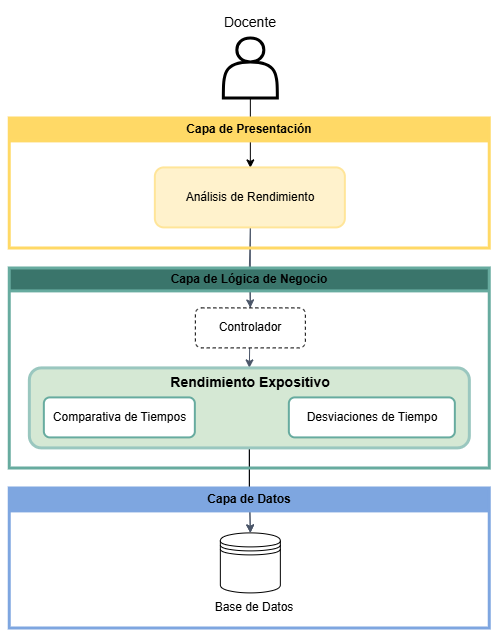
\includegraphics[width=0.9\textwidth]{TT-II/Fig28.png}
    \caption{Arquitectura del Prototipo 3.}
    \label{fig:arquitectura-prototipo-3}
\end{figure}

\subsubsection*{Diagrama de componentes del Prototipo 3}
\addcontentsline{toc}{subsubsection}{\protect\ttiiTOC{Diagrama de componentes del Prototipo 3}}

El diagrama de componentes del prototipo 3 detalla la organización interna del módulo de análisis de rendimiento a nivel de archivos de software, mostrando cómo se distribuyen las responsabilidades entre los componentes que lo conforman y las relaciones de uso entre ellos. A diferencia de los prototipos anteriores, cuyas capas de presentación agrupan componentes orientados a la acción ---carga, análisis y exposición---, el prototipo 3 reorganiza esta capa en torno a la consulta e interpretación de los datos registrados durante las sesiones de exposición previas.

La capa de presentación se organiza en torno a un único módulo denominado \textit{Analytics Post-Class}, que agrupa los componentes visuales del informe de rendimiento. El orquestador de este módulo es \texttt{performance\_gui.py}, que coordina tres paneles especializados: \texttt{performance\_\allowbreak summary\_\allowbreak panel.py}, responsable de desplegar los indicadores globales de la sesión ---etiqueta de desempeño, tiempo recomendado por la IA, tiempo estimado por el docente, duración real y desviación porcentual---; \texttt{performance\_chart\_panel.py}, que renderiza la gráfica de tendencia de tiempo por diapositiva con las dos series comparativas y los controles de filtrado por grupo; y \texttt{performance\_\allowbreak deviations\_\allowbreak panel.py}, que presenta el panel de desviaciones clasificando las diapositivas que excedieron o no alcanzaron el tiempo recomendado por la IA. La navegación hacia este módulo desde el resto del prototipo se gestiona a través de \texttt{navigator.py}.

La capa de lógica de negocio mantiene el módulo \textit{Controller} con los mismos dos controladores de los prototipos anteriores: \texttt{presentation\_controller.py}, que en este contexto coordina la recuperación de los datos de sesión y el cálculo de las comparativas y desviaciones de tiempo, y \texttt{subject\_controller.py}, que provee la información de la unidad de aprendizaje asociada a la presentación consultada.

La capa de infraestructura no participa en este prototipo, dado que el informe de rendimiento se construye íntegramente a partir de los datos locales almacenados en sesiones previas, sin requerir comunicación con la API de Google Gemini.

La capa de datos mantiene la misma estructura de los prototipos anteriores: \texttt{persistence.py} y \texttt{queries.py} coordinados por \texttt{database\_manager.py}, que administra todas las operaciones de consulta sobre la base de datos \texttt{ai\_analyzer.db}. En este prototipo las operaciones son exclusivamente de lectura, recuperando los registros de tiempos por diapositiva, tiempo total de sesión, grupo asociado y tiempo estimado generados durante las exposiciones del prototipo 2.

La Figura \ref{fig:componentes-prototipo-3} presenta el diagrama de componentes descrito.

\begin{figure}[!htbp]
    \centering
    \IfGraphicsExists{TT-II/Fig29}{%
        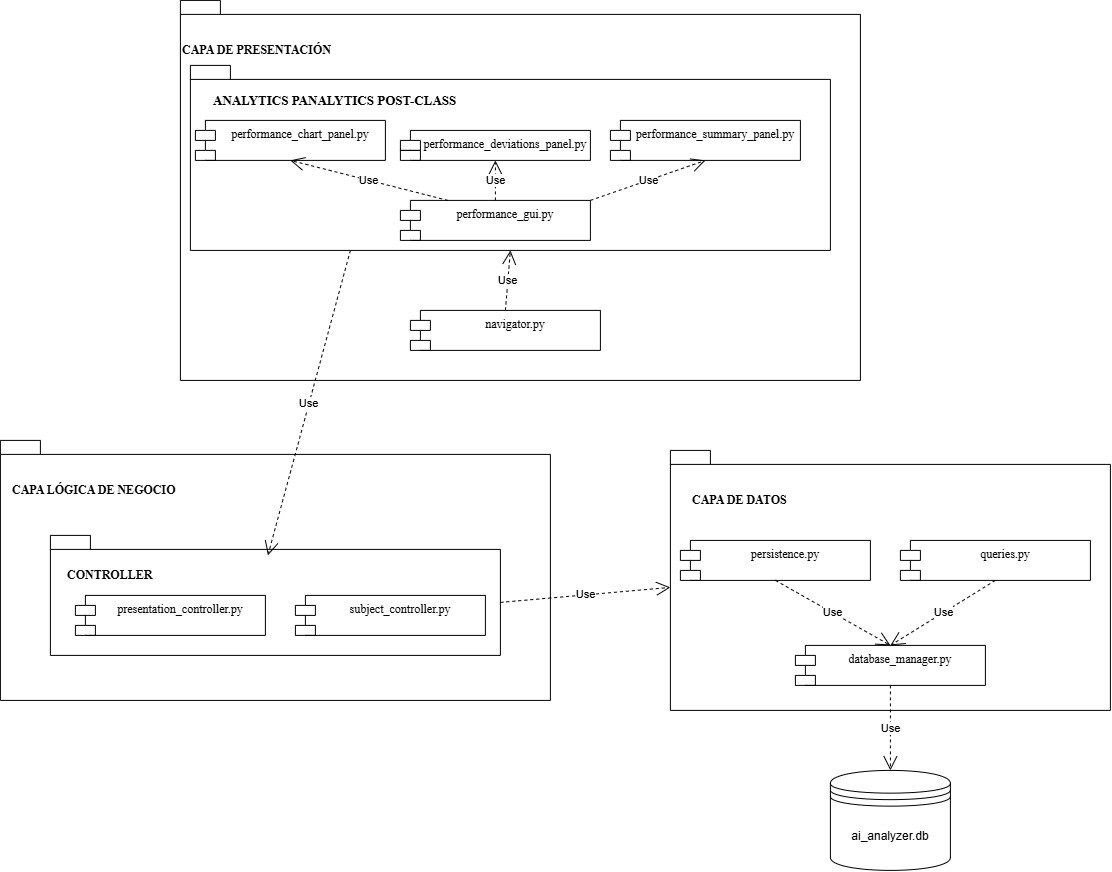
\includegraphics[width=0.95\textwidth]{TT-II/Fig29}%
    }{%
        \fbox{\parbox[c][8cm][c]{0.9\textwidth}{\centering
        Espacio reservado para el diagrama de componentes del prototipo 3.\\[0.45cm]
        Nombre del archivo: \texttt{Fig29.JPG}\\[0.15cm]
        Carpeta: \texttt{TT-II}\\[0.15cm]
        Ruta: \nolinkurl{TT-II/Fig29.JPG}}}%
    }
    \caption{Diagrama de Componentes del Prototipo 3.}
    \label{fig:componentes-prototipo-3}
\end{figure}
\clearpage

\subsubsection*{Diseño de la interfaz del Prototipo 3}
\addcontentsline{toc}{subsubsection}{\protect\ttiiTOC{Diseño de la interfaz del Prototipo 3}}

El diseño de la interfaz del prototipo 3 tiene como criterio central la claridad interpretativa: el docente debe poder leer, comparar y comprender los resultados de su exposición de un solo vistazo, sin necesidad de navegar entre múltiples pantallas ni interpretar datos crudos sin contexto. Para ello, la interfaz organiza el informe de rendimiento en tres bloques visuales jerárquicos que van de lo general a lo particular: primero los indicadores globales de la sesión, después la tendencia temporal por diapositiva y finalmente el detalle de las desviaciones individuales. Esta progresión permite al docente obtener una lectura rápida del desempeño general y profundizar únicamente en los puntos que requieren su atención.

A diferencia de los prototipos anteriores, cuyas interfaces están orientadas a la acción ---cargar, analizar, exponer---, la interfaz del prototipo 3 es predominantemente consultiva. El docente no ejecuta procesos, sino que interpreta resultados, por lo que el diseño prioriza la legibilidad de los datos, la diferenciación visual entre series comparativas y la accesibilidad del panel de desviaciones sin interrumpir la lectura del informe principal. Los diseños preliminares que se presentan a continuación representan la distribución visual de los elementos principales del informe y los controles de filtrado por grupo disponibles para el docente.

Una vez que una presentación ha sido expuesta y cuenta con una sesión registrada, se habilita el botón \textit{Ver rendimiento}, mediante el cual el docente puede consultar el informe correspondiente, como se muestra en la Figura \ref{fig:interfaz-prototipo-3-ver-rendimiento}.

\begin{figure}[!htbp]
    \centering
    \IfGraphicsExists{TT-II/Fig30}{%
        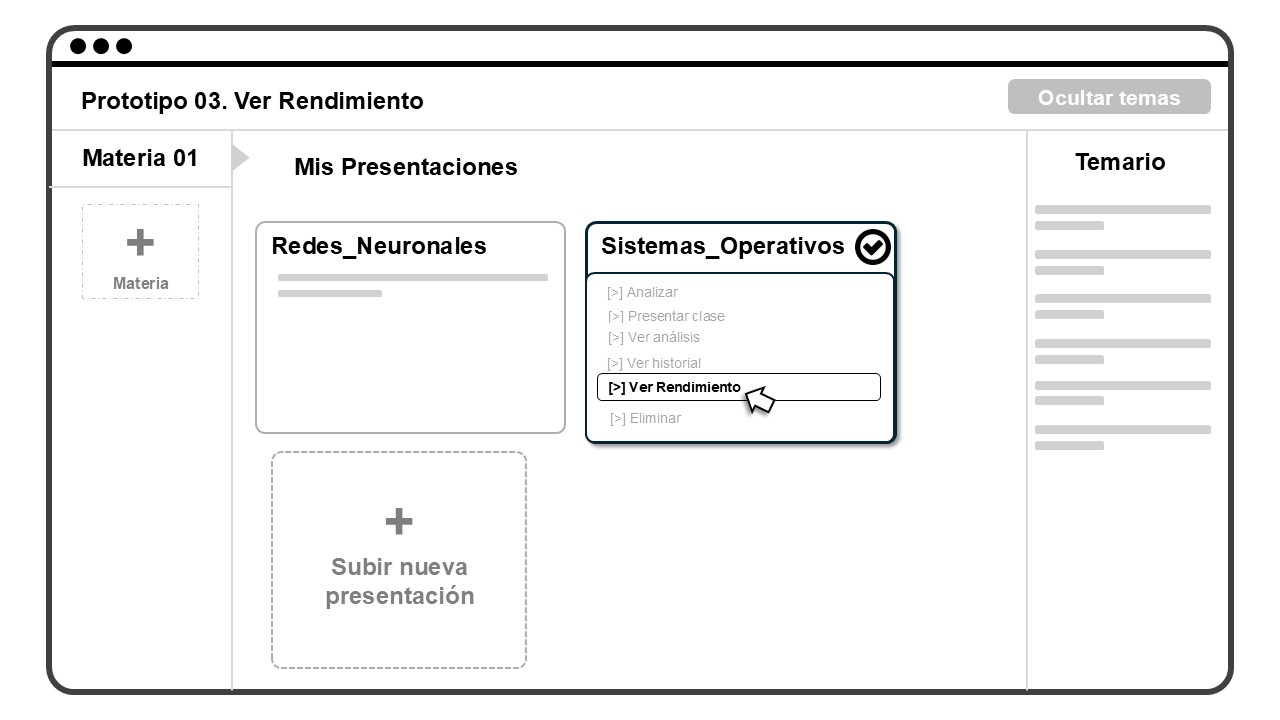
\includegraphics[width=0.8\textwidth]{TT-II/Fig30}%
    }{%
        \fbox{\parbox[c][6cm][c]{0.8\textwidth}{\centering
        Espacio reservado para la interfaz con el botón \textit{Ver rendimiento} habilitado.\\[0.45cm]
        Nombre del archivo: \texttt{Fig30.JPG}\\[0.15cm]
        Carpeta: \texttt{TT-II}\\[0.15cm]
        Ruta: \nolinkurl{TT-II/Fig30.JPG}}}%
    }
    \caption{Botón \textit{Ver rendimiento} habilitado después de registrar una sesión de exposición.}
    \label{fig:interfaz-prototipo-3-ver-rendimiento}
\end{figure}

Al seleccionar \textit{Ver rendimiento}, se abre el panel del informe de la sesión. En este se presenta una gráfica comparativa de los tiempos de exposición por diapositiva, que contrasta el tiempo real registrado con el tiempo recomendado por la IA. Asimismo, se muestran tarjetas informativas con la recopilación de los indicadores globales de la sesión, como se observa en la Figura \ref{fig:interfaz-prototipo-3-informe}.

\begin{figure}[!htbp]
    \centering
    \IfGraphicsExists{TT-II/Fig31}{%
        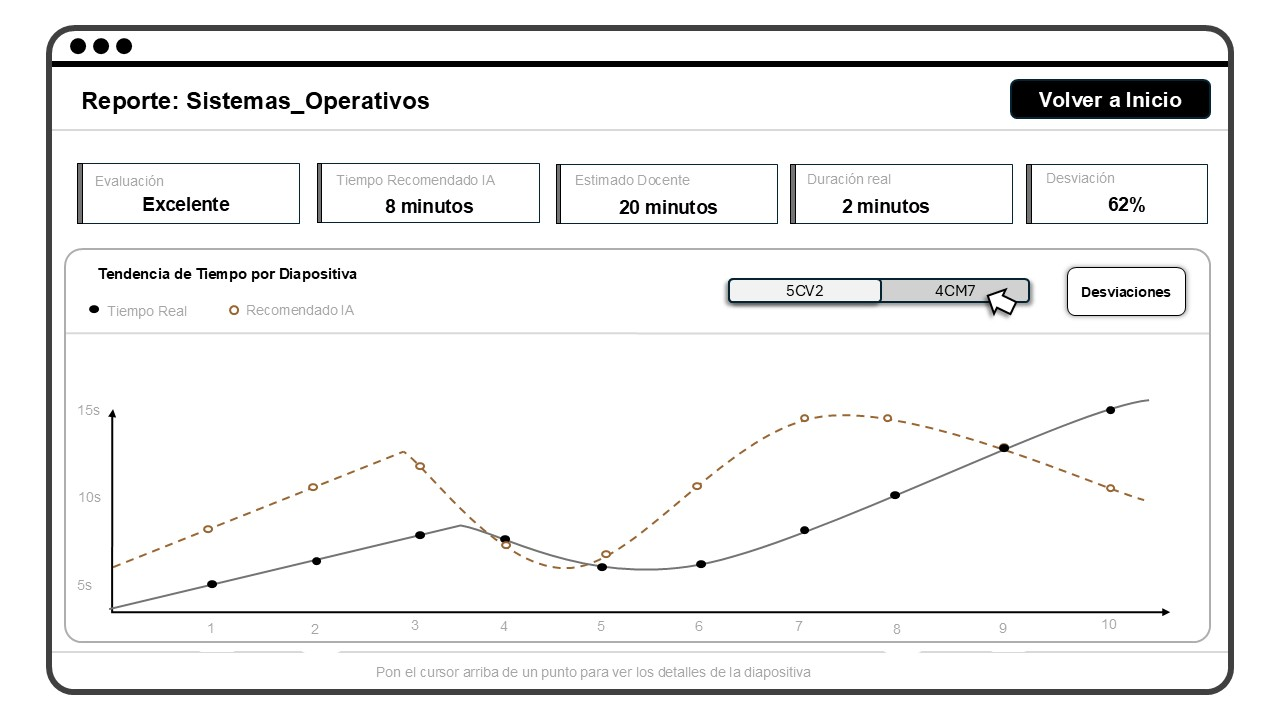
\includegraphics[width=0.8\textwidth]{TT-II/Fig31}%
    }{%
        \fbox{\parbox[c][6cm][c]{0.8\textwidth}{\centering
        Espacio reservado para el panel de rendimiento con la gráfica comparativa y las tarjetas informativas.\\[0.45cm]
        Nombre del archivo: \texttt{Fig31.JPG}\\[0.15cm]
        Carpeta: \texttt{TT-II}\\[0.15cm]
        Ruta: \nolinkurl{TT-II/Fig31.JPG}}}%
    }
    \caption{Informe de rendimiento con indicadores globales y comparación del tiempo real frente al recomendado por la IA.}
    \label{fig:interfaz-prototipo-3-informe}
\end{figure}

En este panel también es posible consultar el rendimiento por grupo. Cuando el docente selecciona un grupo diferente, los indicadores y la gráfica se actualizan para mostrar únicamente los datos recopilados durante la sesión correspondiente a ese grupo, como se ilustra en la Figura \ref{fig:interfaz-prototipo-3-grupo}.

\begin{figure}[!htbp]
    \centering
    \IfGraphicsExists{TT-II/Fig32}{%
        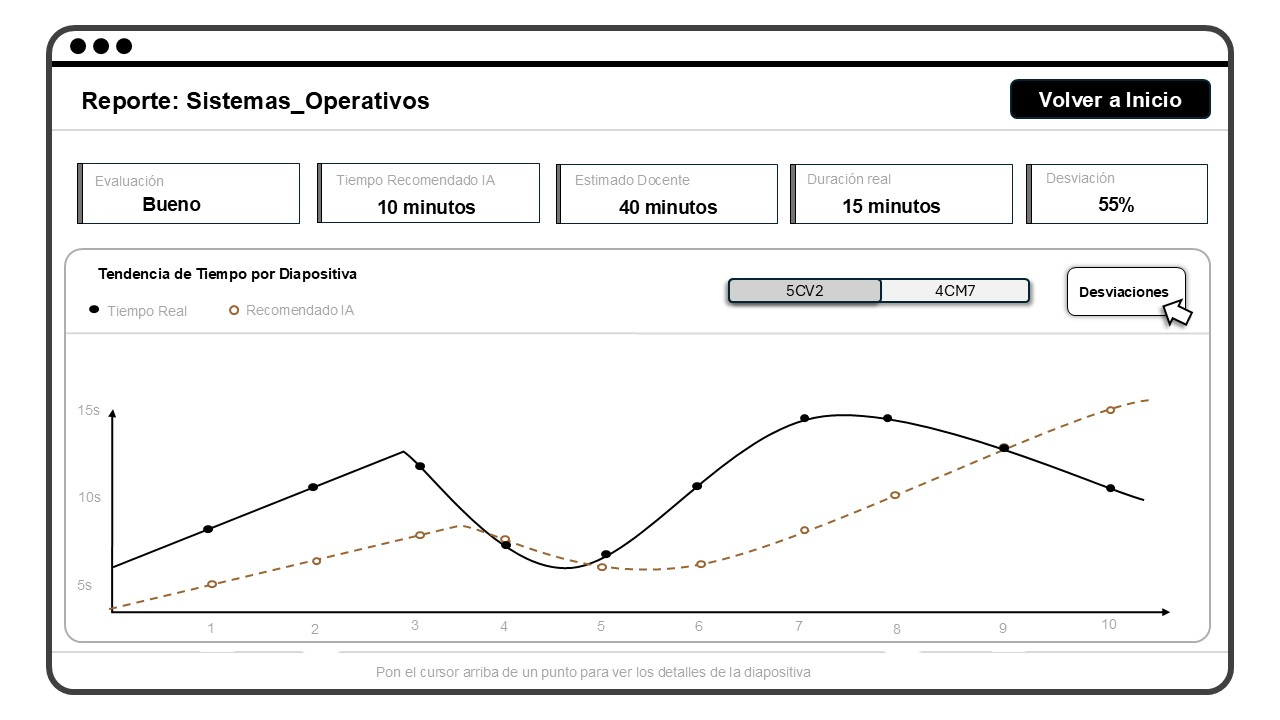
\includegraphics[width=0.8\textwidth]{TT-II/Fig32}%
    }{%
        \fbox{\parbox[c][6cm][c]{0.8\textwidth}{\centering
        Espacio reservado para la consulta del rendimiento mediante el selector de grupos.\\[0.45cm]
        Nombre del archivo: \texttt{Fig32.JPG}\\[0.15cm]
        Carpeta: \texttt{TT-II}\\[0.15cm]
        Ruta: \nolinkurl{TT-II/Fig32.JPG}}}%
    }
    \caption{Consulta y actualización del informe de rendimiento de acuerdo con el grupo seleccionado.}
    \label{fig:interfaz-prototipo-3-grupo}
\end{figure}

Finalmente, el botón \textit{Desviaciones} abre una ventana con el informe de las diapositivas cuya duración fue significativamente menor o mayor en comparación con el tiempo recomendado por la IA. Esta vista permite identificar los segmentos de la exposición que requieren atención, como se muestra en la Figura \ref{fig:interfaz-prototipo-3-desviaciones}.

\begin{figure}[!htbp]
    \centering
    \IfGraphicsExists{TT-II/Fig33}{%
        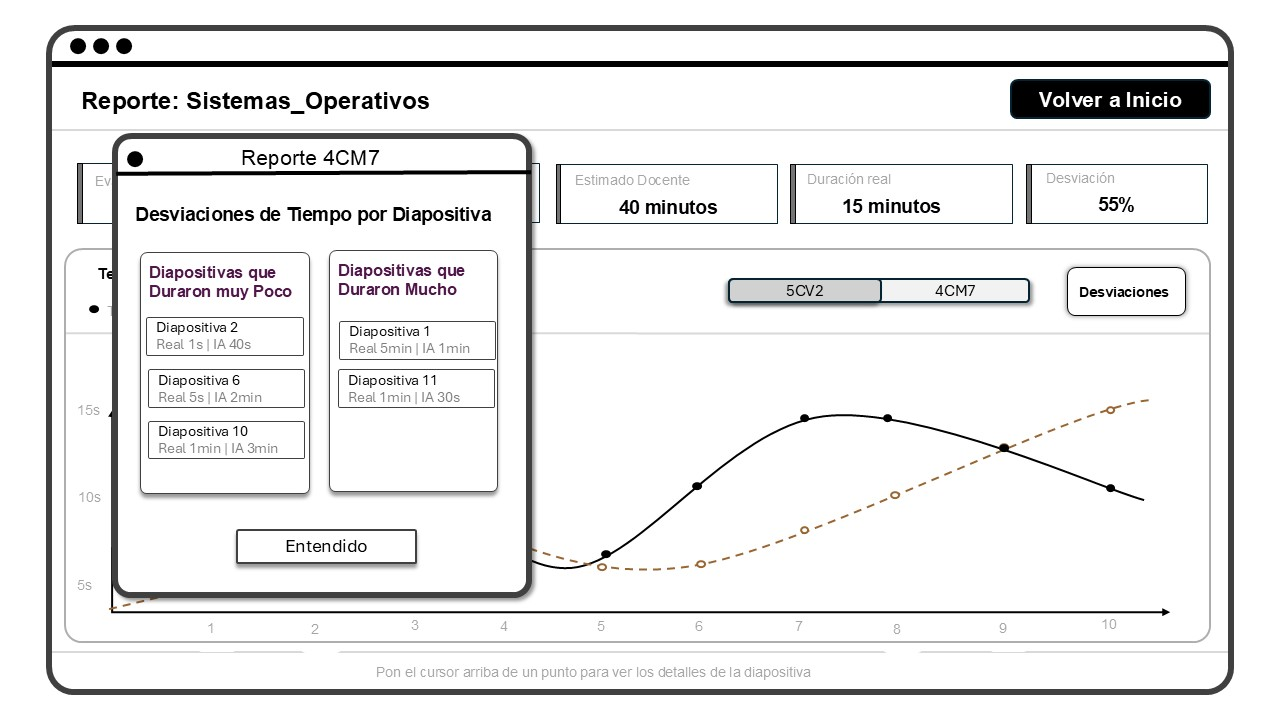
\includegraphics[width=0.8\textwidth]{TT-II/Fig33}%
    }{%
        \fbox{\parbox[c][6cm][c]{0.8\textwidth}{\centering
        Espacio reservado para la ventana de desviaciones de tiempo por diapositiva.\\[0.45cm]
        Nombre del archivo: \texttt{Fig33.JPG}\\[0.15cm]
        Carpeta: \texttt{TT-II}\\[0.15cm]
        Ruta: \nolinkurl{TT-II/Fig33.JPG}}}%
    }
    \caption{Informe de las diapositivas cuya duración fue menor o mayor que el tiempo recomendado por la IA.}
    \label{fig:interfaz-prototipo-3-desviaciones}
\end{figure}

\clearpage
\subsubsection*{Desarrollo del Prototipo 3}
\addcontentsline{toc}{subsubsection}{\protect\ttiiTOC{Desarrollo del Prototipo 3}}

La fase de desarrollo del prototipo 3 comprende la implementación de los módulos definidos en la arquitectura de cuatro capas descrita en la sección anterior, abarcando desde la recuperación y el procesamiento de los datos de sesión registrados por el prototipo 2 hasta el cálculo de las comparativas de tiempo, la identificación de desviaciones por diapositiva y la visualización del informe de rendimiento completo.

Con el propósito de documentar el comportamiento del prototipo 3 e ilustrar la interacción entre sus componentes durante la ejecución de los flujos principales, se elaboraron diagramas de secuencia para cada una de las funcionalidades centrales del módulo de análisis de rendimiento.

Los flujos documentados mediante diagramas de secuencia corresponden a las siguientes operaciones: acceso al informe de rendimiento y validación de sesiones registradas, ensamblaje del dashboard, cambio de grupo, consulta de información mediante \textit{tooltip} y desplazamiento mediante \textit{scroll}, reporte de desviaciones mediante una ventana modal, y salida y restauración del estado anterior. Cada diagrama contempla tanto el flujo principal de éxito como las variantes de excepción más relevantes, entre las que se incluye el intento de acceso al informe desde una presentación que no cuenta con sesiones de exposición registradas.

\begin{figure}[!htbp]
    \centering
    \IfGraphicsExists{TT-II/Fig34}{%
        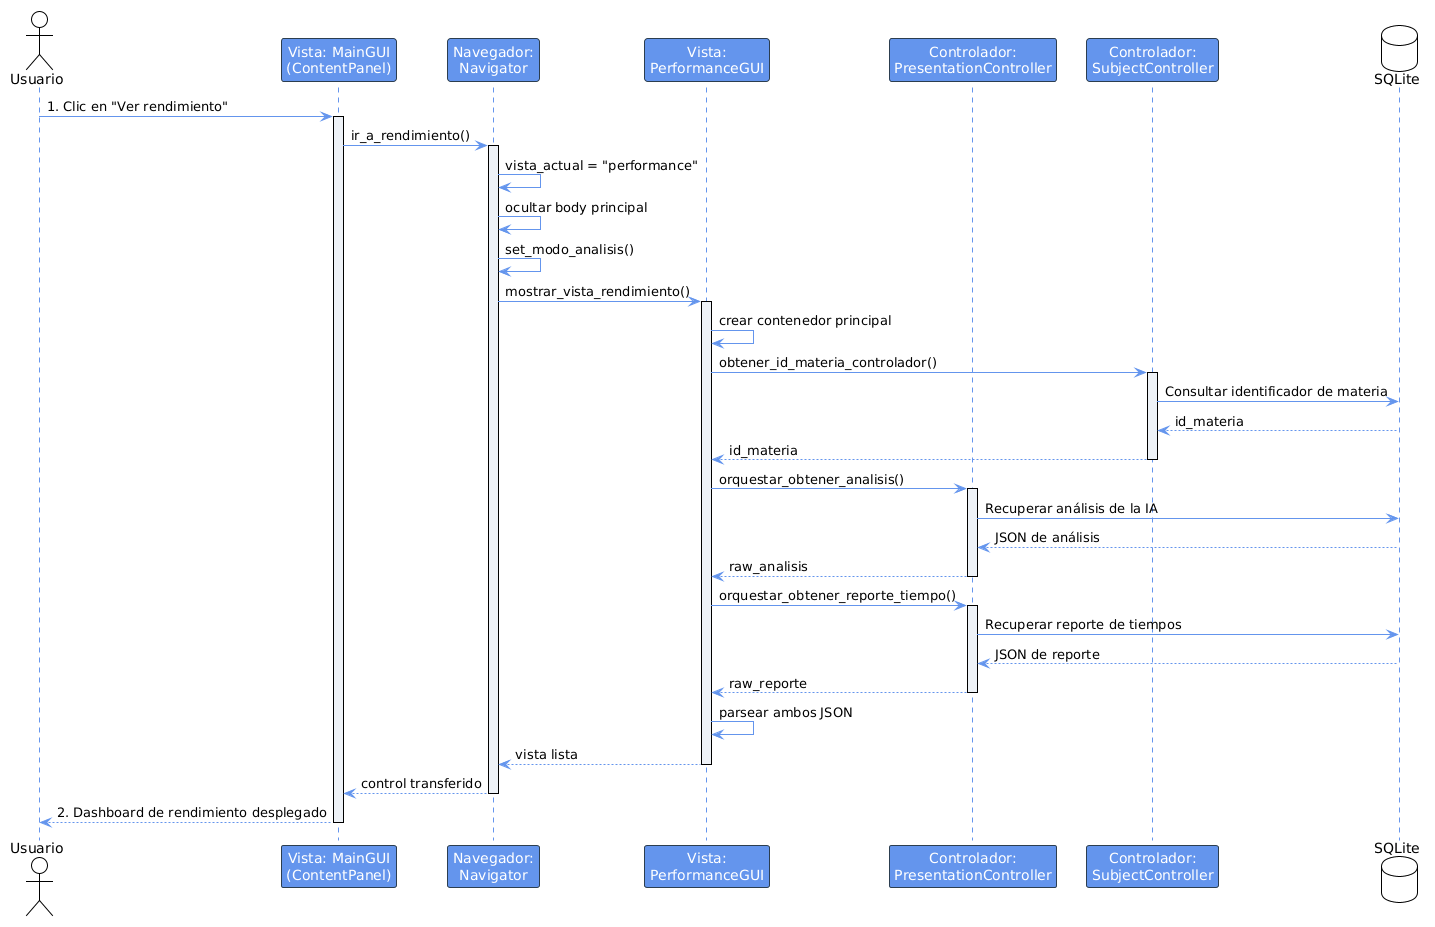
\includegraphics[width=0.95\textwidth]{TT-II/Fig34}%
    }{%
        \fbox{\parbox[c][8cm][c]{0.9\textwidth}{\centering
        Espacio reservado para el diagrama de secuencia de entrada a la vista.\\[0.45cm]
        Nombre del archivo: \texttt{Fig34.png}\\[0.15cm]
        Carpeta: \texttt{TT-II}\\[0.15cm]
        Ruta: \nolinkurl{TT-II/Fig34.png}}}%
    }
    \caption{Diagrama de secuencia de la entrada a la vista y la validación de sesiones registradas.}
    \label{fig:secuencia-prototipo-3-entrada-vista}
\end{figure}

\begin{figure}[!htbp]
    \centering
    \IfGraphicsExists{TT-II/Fig35}{%
        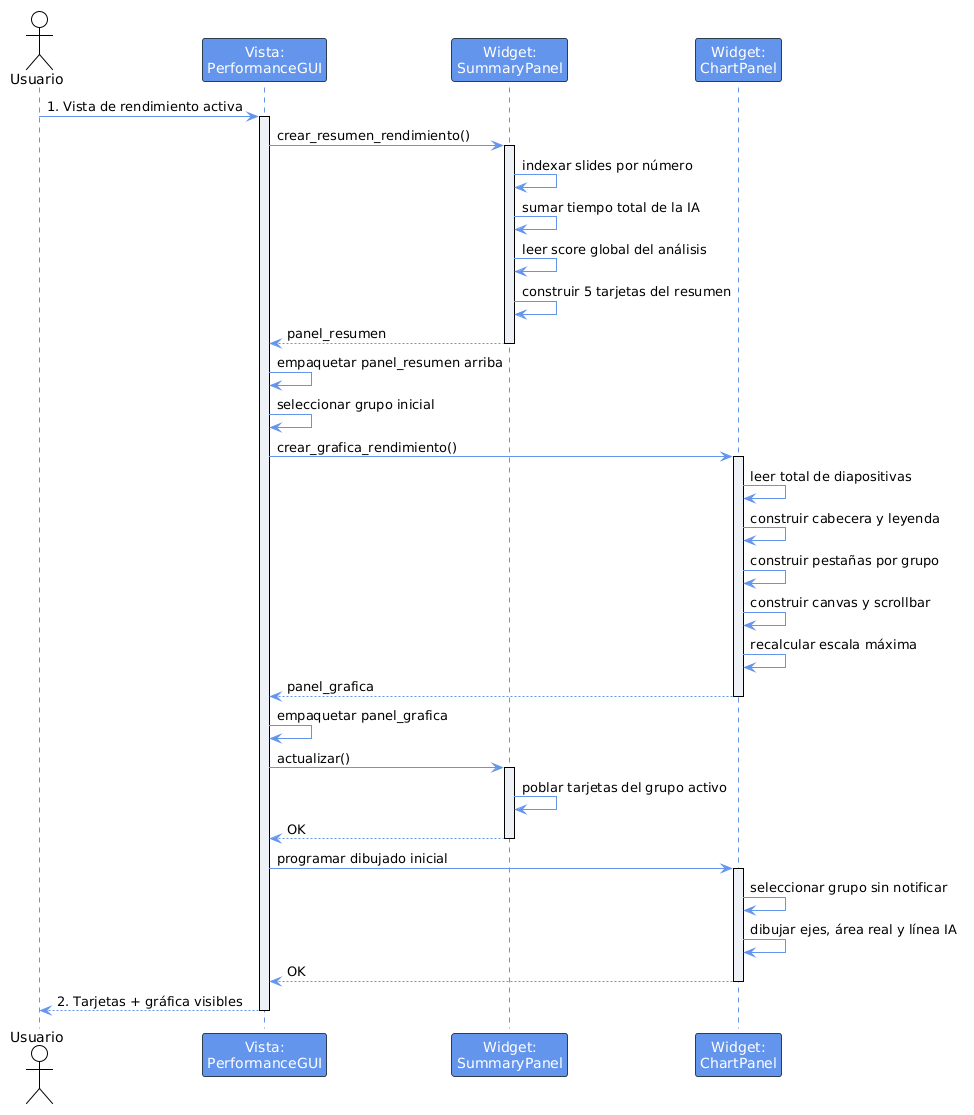
\includegraphics[width=0.95\textwidth]{TT-II/Fig35}%
    }{%
        \fbox{\parbox[c][8cm][c]{0.9\textwidth}{\centering
        Espacio reservado para el diagrama de secuencia del ensamblaje del dashboard.\\[0.45cm]
        Nombre del archivo: \texttt{Fig35.png}\\[0.15cm]
        Carpeta: \texttt{TT-II}\\[0.15cm]
        Ruta: \nolinkurl{TT-II/Fig35.png}}}%
    }
    \caption{Diagrama de secuencia del ensamblaje del dashboard de rendimiento.}
    \label{fig:secuencia-prototipo-3-ensamblaje-dashboard}
\end{figure}

\begin{figure}[!htbp]
    \centering
    \IfGraphicsExists{TT-II/Fig36}{%
        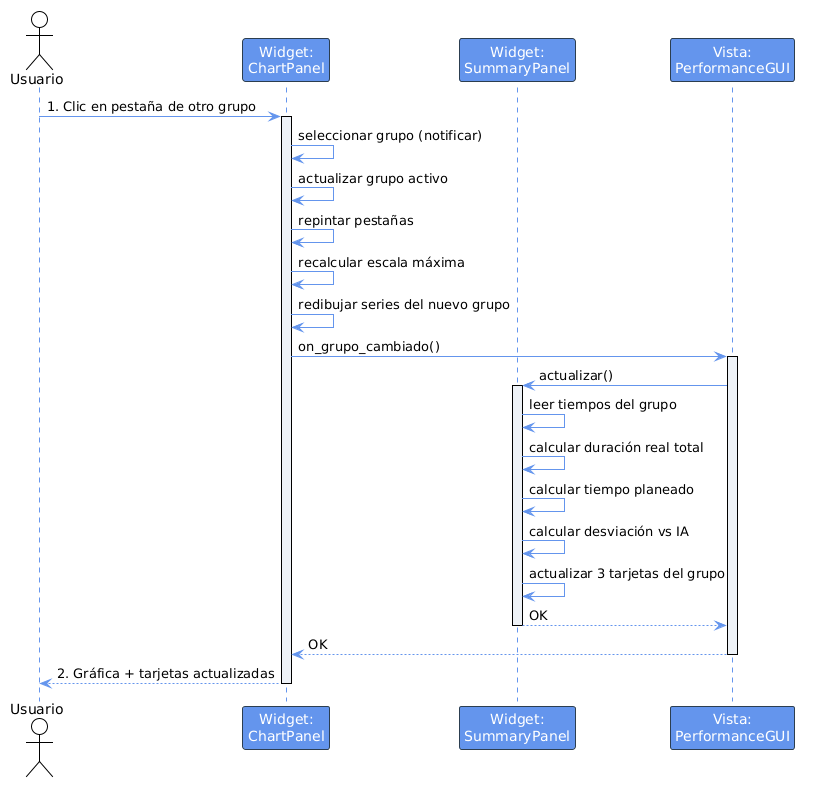
\includegraphics[width=0.95\textwidth]{TT-II/Fig36}%
    }{%
        \fbox{\parbox[c][8cm][c]{0.9\textwidth}{\centering
        Espacio reservado para el diagrama de secuencia del cambio de grupo.\\[0.45cm]
        Nombre del archivo: \texttt{Fig36.png}\\[0.15cm]
        Carpeta: \texttt{TT-II}\\[0.15cm]
        Ruta: \nolinkurl{TT-II/Fig36.png}}}%
    }
    \caption{Diagrama de secuencia del cambio de grupo y la actualización de los datos del informe.}
    \label{fig:secuencia-prototipo-3-cambio-grupo}
\end{figure}

\begin{figure}[!htbp]
    \centering
    \IfGraphicsExists{TT-II/Fig37}{%
        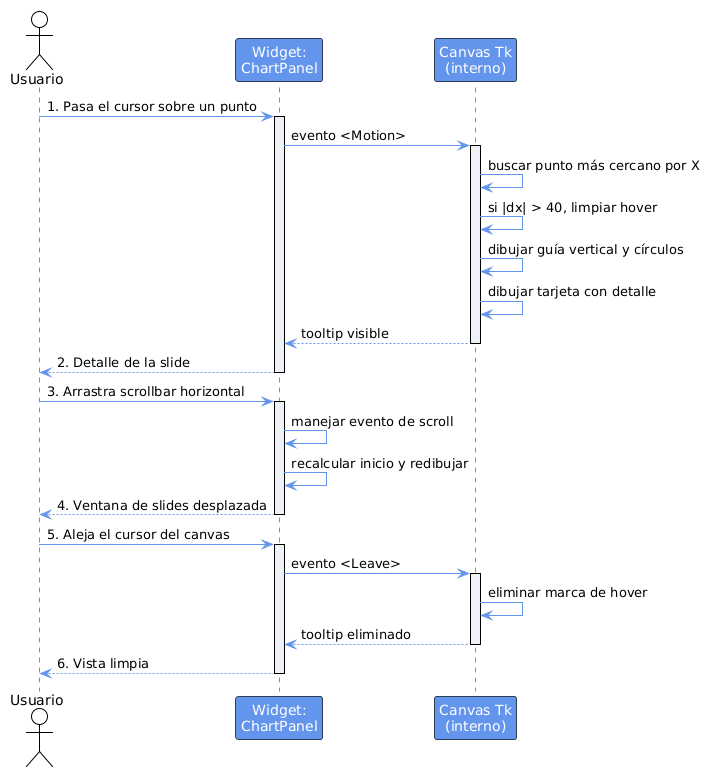
\includegraphics[width=0.95\textwidth]{TT-II/Fig37}%
    }{%
        \fbox{\parbox[c][8cm][c]{0.9\textwidth}{\centering
        Espacio reservado para el diagrama de secuencia de \textit{tooltip} y \textit{scroll}.\\[0.45cm]
        Nombre del archivo: \texttt{Fig37.png}\\[0.15cm]
        Carpeta: \texttt{TT-II}\\[0.15cm]
        Ruta: \nolinkurl{TT-II/Fig37.png}}}%
    }
    \caption{Diagrama de secuencia de la consulta mediante \textit{tooltip} y el desplazamiento mediante \textit{scroll}.}
    \label{fig:secuencia-prototipo-3-tooltip-scroll}
\end{figure}

\begin{figure}[!htbp]
    \centering
    \IfGraphicsExists{TT-II/Fig38}{%
        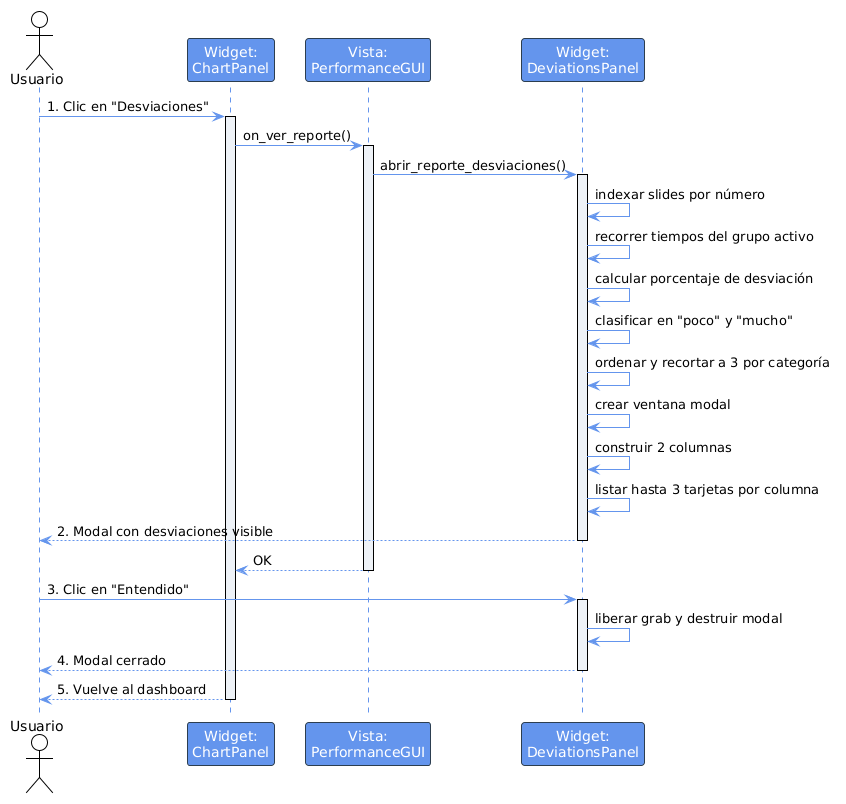
\includegraphics[width=0.95\textwidth]{TT-II/Fig38}%
    }{%
        \fbox{\parbox[c][8cm][c]{0.9\textwidth}{\centering
        Espacio reservado para el diagrama de secuencia del reporte de desviaciones.\\[0.45cm]
        Nombre del archivo: \texttt{Fig38.png}\\[0.15cm]
        Carpeta: \texttt{TT-II}\\[0.15cm]
        Ruta: \nolinkurl{TT-II/Fig38.png}}}%
    }
    \caption{Diagrama de secuencia del reporte de desviaciones mediante una ventana modal.}
    \label{fig:secuencia-prototipo-3-reporte-desviaciones}
\end{figure}

\begin{figure}[!htbp]
    \centering
    \IfGraphicsExists{TT-II/Fig39}{%
        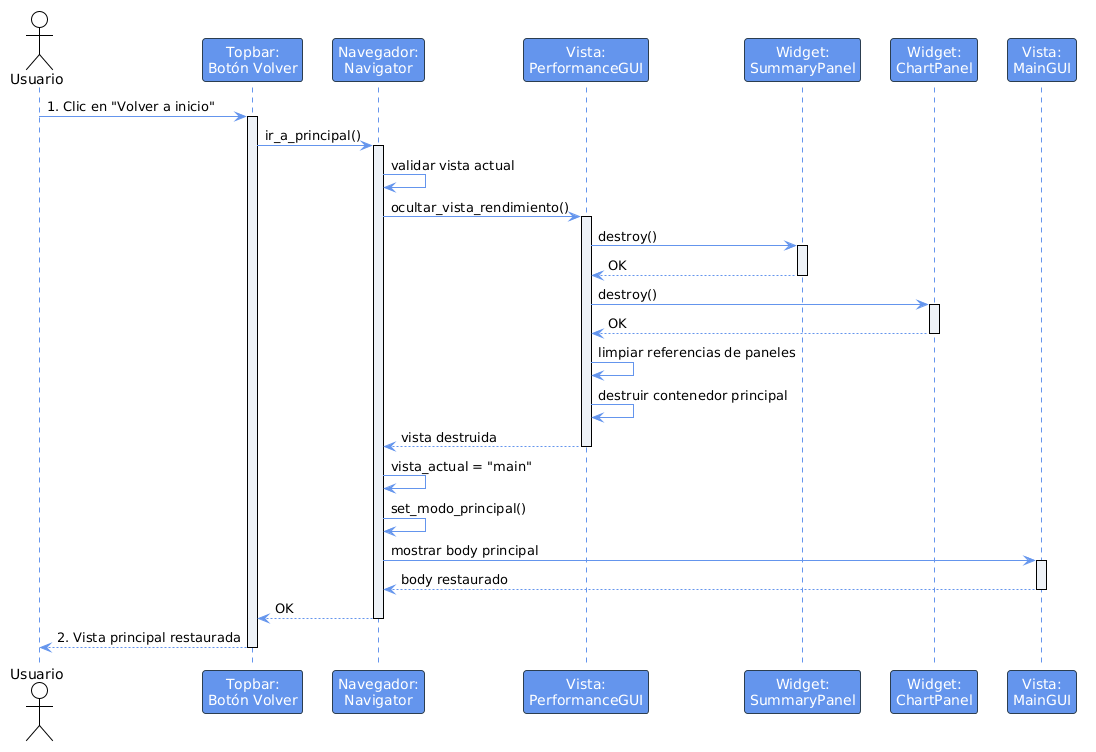
\includegraphics[width=0.95\textwidth]{TT-II/Fig39}%
    }{%
        \fbox{\parbox[c][8cm][c]{0.9\textwidth}{\centering
        Espacio reservado para el diagrama de secuencia de salida y restauración.\\[0.45cm]
        Nombre del archivo: \texttt{Fig39.png}\\[0.15cm]
        Carpeta: \texttt{TT-II}\\[0.15cm]
        Ruta: \nolinkurl{TT-II/Fig39.png}}}%
    }
    \caption{Diagrama de secuencia de la salida de la vista y la restauración del estado anterior.}
    \label{fig:secuencia-prototipo-3-salida-restauracion}
\end{figure}


\clearpage
\subsubsection*{Protocolo de Pruebas del Prototipo 3}
\addcontentsline{toc}{subsubsection}{\protect\ttiiTOC{Protocolo de Pruebas del Prototipo 3}}

Para facilitar la trazabilidad de las pruebas del prototipo 3, se utiliza un prefijo de tres letras y un número consecutivo. La Tabla \ref{tab:nomenclatura-pruebas-prototipo-3} presenta las categorías empleadas.

\begin{table}[H]
\centering
\renewcommand{\arraystretch}{1.2}
\ttstyle
\begin{tabularx}{\textwidth}{>{\centering\arraybackslash}p{1.5cm}p{4.6cm}X}
\toprule
\textbf{Sigla} & \textbf{Módulo o categoría} & \textbf{Significado dentro del protocolo} \\
\midrule
PRF & Dashboard de rendimiento & Entrada a la vista, recuperación de los JSON y construcción de las tarjetas de resumen. \\
\hairrule
GRF & Gráfica de tendencias & Series de tiempo, \textit{tooltip}, desplazamiento horizontal y pestañas de grupo. \\
\hairrule
DVS & Reporte de desviaciones & Apertura del modal, cálculo de porcentajes y clasificación de diapositivas. \\
\hairrule
INT & Integridad & Consistencia entre el análisis, el reporte de tiempos y la base de datos. \\
\hairrule
USR & Pruebas de usuario & Escenarios derivados de la interacción directa con el dashboard. \\
\bottomrule
\end{tabularx}
\caption{Nomenclatura de los identificadores de las pruebas del prototipo 3.}
\label{tab:nomenclatura-pruebas-prototipo-3}
\end{table}

\clearpage
\textbf{Módulo: Dashboard de Rendimiento}

\textbf{Objetivo:} Validar la recuperación del análisis de la IA y del reporte de tiempos, así como la construcción de las tarjetas de resumen y la gráfica de tendencias.

\textbf{Descripción del flujo:}
\begin{enumerate}
\item Acceder mediante «Ver rendimiento», disponible solo si existe al menos una sesión registrada.
\item Configurar la interfaz en modo secundario.
\item Resolver el identificador de la materia.
\item Recuperar los JSON de análisis y tiempos.
\item Construir las cinco tarjetas de resumen y la gráfica.
\item Restaurar la vista mediante «Volver a inicio».
\end{enumerate}

\textbf{Arquitectura del módulo:}
\begin{verbatim}
Dashboard de Rendimiento
|-- views/performance_gui.py
|-- views/navigator.py
|-- widgets/performance_mode/
|   |-- performance_summary_panel.py
|   |-- performance_chart_panel.py
|   +-- performance_deviations_panel.py
|-- controller/
|   |-- presentation_controller.py
|   +-- subject_controller.py
+-- data/queries.py, database_manager.py
\end{verbatim}

\textbf{Componentes que probar:}
\begin{table}[H]
\centering
\ttstyle
\begin{tabular}{L{0.30\textwidth}L{0.16\textwidth}L{0.44\textwidth}}
\toprule
\textbf{Componente} & \textbf{Tipo} & \textbf{Descripción} \\
\midrule
Vista de rendimiento & UI/Frontend & Orquesta la carga de los JSON y monta los paneles. \\
\hairrule
Tarjetas de resumen & UI/Frontend & Muestran calificación, tiempos y desviación. \\
\hairrule
Controladores & Backend & Obtienen el análisis, el reporte y el identificador de la materia. \\
\hairrule
Consultas & Base de datos & Extraen los datos desde \texttt{Historial\_de\_Versiones}. \\
\bottomrule
\end{tabular}
\caption{Componentes del módulo de dashboard de rendimiento.}
\label{tab:componentes-modulo-dashboard}
\end{table}

\textbf{Cobertura de pruebas --- Dashboard de Rendimiento:}
{\ttpruebasetup
\begin{longtable}{@{}p{\linewidth}@{}}
\ttcase{PRF-01}{Entrada a la vista}{Seleccionar «Ver rendimiento».}{Se despliega el dashboard.}{Sí}{Al seleccionar la opción, la vista principal es reemplazada por el dashboard de rendimiento, que muestra el panel de tarjetas de resumen en la parte superior y la gráfica de tendencia de tiempo por diapositiva en el área central.}
\ttcase{PRF-02}{Carga de análisis}{Recuperar la evaluación generada durante el análisis.}{Se recupera el análisis de la presentación.}{Sí}{Al abrir el dashboard, los datos del análisis de la presentación quedan disponibles de forma inmediata. El número de diapositivas mostrado en los indicadores coincide con el total evaluado durante el análisis previo.}
\ttcase{PRF-03}{Carga de tiempos}{Abrir una presentación con sesiones.}{Se recupera el reporte de tiempos.}{Sí}{Al abrir el dashboard, la pestaña del grupo con sesiones registradas aparece disponible en la gráfica, mostrando la duración real acumulada de todas sus sesiones.}
\ttcase{PRF-04}{Resumen con datos}{Revisar las cinco tarjetas.}{Se muestran todos los indicadores.}{Sí}{Las cinco tarjetas muestran los siguientes valores: «Planeó docente» con el tiempo estimado ingresado por el docente al iniciar la sesión, «Duración real» con el tiempo total registrado durante la exposición e indicando cuántas diapositivas fueron presentadas, «Tiempo IA» con el tiempo recomendado por el análisis, «Desviación» con el porcentaje de diferencia entre el tiempo real y el recomendado, y «Calificación» con la etiqueta de desempeño global de la presentación.}
\ttcase{PRF-05}{Reporte sin grupos}{Solicitar el reporte de rendimiento de una presentación analizada que aún no se ha expuesto a ningún grupo.}{Se informa que es necesario exponer la presentación al menos una vez ante un grupo.}{Sí}{Para generar el reporte se requiere una presentación analizada y al menos una sesión de exposición registrada para un grupo. Al intentar consultarlo sin sesiones, aparece el modal «Sin datos de rendimiento», que indica que primero se debe exponer la presentación al menos una vez ante un grupo. El prototipo bloquea el acceso de forma controlada, tal como se espera.}
\ttcase{PRF-06}{Sin análisis}{Solicitar la presentación o el reporte de rendimiento de una presentación que no cuenta con análisis.}{Se bloquea el flujo y se informa que el análisis es un requisito previo.}{Sí}{Sin análisis no se puede iniciar la presentación; por lo tanto, tampoco se genera una sesión ni existe información para el reporte de rendimiento. Al intentar presentar, aparece el modal «Análisis requerido» con el mensaje «Para poder presentar la clase, primero debes ejecutar el Análisis de IA sobre esta versión». El prototipo bloquea el flujo de forma controlada, tal como se espera.}
\ttcase{PRF-07}{Tiempo IA}{Mostrar el tiempo de exposición recomendado.}{El total coincide con la suma de los tiempos por diapositiva.}{Sí}{Cuando el análisis no incluye un tiempo total de exposición calculado de forma directa, el dashboard suma los tiempos recomendados de cada diapositiva individual y muestra el resultado en la tarjeta «Tiempo IA».}
\ttcase{PRF-08}{Grupo inicial}{Abrir una presentación con dos grupos.}{El dashboard selecciona el primer grupo disponible.}{Sí}{Al abrir el dashboard con dos grupos registrados, la primera pestaña disponible queda seleccionada por defecto y el resumen y la gráfica muestran los datos correspondientes a ese grupo.}
\ttcase{PRF-09}{Análisis corrupto}{Introducir un análisis con formato inválido.}{Se controla el error y la vista continúa funcionando.}{Sí}{Cuando el archivo de análisis contiene un formato inválido, el dashboard no muestra ningún error al usuario. El análisis queda vacío y la vista permanece funcional, mostrando los indicadores disponibles en estado de ausencia de datos.}
\ttcase{PRF-10}{Reporte corrupto}{Abrir el reporte de rendimiento con un reporte de tiempos inválido, aunque existan sesiones en el historial.}{El prototipo bloquea el acceso al reporte y muestra el aviso «Aún no se ha presentado esta clase...» cuando no logra leer el reporte de tiempos.}{Sí}{Aunque existen sesiones registradas en el historial, el reporte de tiempos con formato inválido no puede leerse y el prototipo bloquea el acceso mostrando el modal «Aún no se ha presentado esta clase...».}
\ttcase{PRF-11}{Regreso al inicio}{Seleccionar «Volver a inicio».}{Se restaura la vista principal.}{Sí}{Al pulsar «Volver a inicio», la vista del dashboard es desmontada y la vista principal con la cuadrícula de presentaciones vuelve a mostrarse sin rastros del informe de rendimiento.}
\ttcase{PRF-12}{Eliminación durante la vista}{Intentar eliminar la presentación desde el dashboard.}{La vista de rendimiento no expone ningún control para eliminar presentaciones.}{Sí}{La vista de rendimiento no expone ningún control de eliminación de presentaciones. No es posible realizar esta acción desde el dashboard.}
\ttcase{PRF-13}{Calificación por etiqueta}{Revisar la tarjeta de calificación.}{Se muestra una etiqueta cualitativa en lugar de un número.}{Sí}{La tarjeta de calificación muestra la etiqueta de desempeño de la presentación en texto, como «Excelente», «Bueno», «Regular» o «Deficiente», en lugar de la puntuación numérica del análisis.}
\ttcase{PRF-14}{Desviación global}{Comparar la duración real con el tiempo recomendado por la IA.}{La tarjeta cambia de color según el nivel de desviación.}{Sí}{La tarjeta «Desviación» muestra el porcentaje de diferencia entre el tiempo real y el recomendado por la IA, y cambia de color según el nivel: naranja cuando el exceso supera el umbral establecido, ámbar cuando el tiempo fue significativamente menor al recomendado, y verde cuando la desviación está dentro del rango aceptable.}
\ttcase{PRF-15}{Diapositivas presentadas}{Observar el subtítulo de la tarjeta «Duración real».}{Indica cuántas diapositivas tienen tiempo real registrado.}{Sí}{El subtítulo de la tarjeta «Duración real» muestra el formato «N/total diapositivas», donde N corresponde al número de diapositivas a las que el docente dedicó tiempo durante la sesión. Con 2 de 4 diapositivas presentadas, el subtítulo mostró «2/4 diapositivas».}
\ttcase{PRF-16}{Tiempo planeado del grupo}{Guardar dos sesiones y abrir el dashboard.}{La tarjeta «Planeó docente» muestra el tiempo de la última sesión.}{Sí}{Cuando un grupo tiene varias sesiones registradas con distintos tiempos estimados, la tarjeta «Planeó docente» muestra el tiempo ingresado en la sesión más reciente. Con sesiones de 30 y 10 minutos, la tarjeta mostró «10m 00s».}
\ttcaselast{PRF-17}{Reapertura del dashboard}{Salir del dashboard y volver a entrar.}{Se reconstruye correctamente sin residuos de la sesión anterior.}{Sí}{Al cerrar el dashboard y volver a abrirlo, los grupos y los datos se cargan nuevamente desde la base de datos y la vista queda en el mismo estado operativo que en la primera apertura, sin datos residuales de la sesión anterior.}
\caption{Casos de prueba del módulo de dashboard de rendimiento.}
\label{tab:casos-prueba-dashboard}
\end{longtable}
}

\clearpage
\textbf{Módulo: Gráfica de Tendencias}

\textbf{Objetivo:} Validar el dibujado de las series de tiempo real y recomendado por la IA, el \textit{tooltip}, el desplazamiento horizontal y la actualización al cambiar de grupo.

\textbf{Descripción del flujo:}
\begin{enumerate}
\item Construir el lienzo, los ejes y la barra de desplazamiento.
\item Dibujar el área real y ambas series.
\item Mostrar el detalle de cada punto al pasar el cursor.
\item Cambiar de grupo y redibujar la gráfica y el resumen.
\item Ajustar el contenido al redimensionar la ventana.
\end{enumerate}

\textbf{Arquitectura del módulo:}
\begin{verbatim}
Gráfica de Tendencias
+-- widgets/performance_mode/performance_chart_panel.py
\end{verbatim}

\textbf{Componentes que probar:}
\begin{table}[H]
\centering
\ttstyle
\begin{tabular}{L{0.30\textwidth}L{0.16\textwidth}L{0.44\textwidth}}
\toprule
\textbf{Componente} & \textbf{Tipo} & \textbf{Descripción} \\
\midrule
Lienzo de la gráfica & UI/Frontend & Dibuja ejes, series, área, puntos y detalles interactivos. \\
\hairrule
Pestañas de grupo & UI/Frontend & Cambian el grupo activo y notifican al resumen. \\
\hairrule
Barra de desplazamiento & UI/Frontend & Permite consultar presentaciones extensas. \\
\hairrule
\textit{Tooltip} & UI/Frontend & Muestra diapositiva, tiempo real y tiempo recomendado. \\
\bottomrule
\end{tabular}
\caption{Componentes del módulo de gráfica de tendencias.}
\label{tab:componentes-modulo-grafica}
\end{table}

\textbf{Cobertura de pruebas --- Gráfica de Tendencias:}
{\ttpruebasetup
\begin{longtable}{@{}p{\linewidth}@{}}
\ttcase{GRF-01}{Dibujado inicial}{Abrir un grupo válido.}{Se dibujan ejes, guías y series.}{Sí}{Al abrir el dashboard con un grupo válido, la gráfica muestra los ejes horizontal y vertical, las líneas de guía de fondo, la serie del tiempo real y la serie del tiempo recomendado por la IA, junto con los puntos correspondientes a cada diapositiva y las etiquetas numéricas en el eje horizontal.}
\ttcase{GRF-02}{Área real}{Revisar el relleno bajo la curva real.}{El área bajo la curva real muestra el color correspondiente a la serie real.}{Sí}{La gráfica muestra un área rellena en color rosado bajo la línea de la serie de tiempo real, diferenciándola visualmente de la serie recomendada por la IA.}
\ttcase{GRF-03}{Serie IA}{Revisar la línea recomendada.}{Se muestra una línea dorada discontinua.}{Sí}{La serie del tiempo recomendado por la IA se representa como una línea dorada con trazo discontinuo, claramente diferenciada de la línea continua de la serie real.}
\ttcase{GRF-04}{Tooltip}{Pasar el cursor sobre un punto.}{Se muestra la guía vertical y el detalle de la diapositiva.}{Sí}{Al posicionar el cursor sobre un punto de la gráfica, aparece una guía vertical y un cuadro informativo que muestra el número de la diapositiva, el tiempo real registrado y el tiempo recomendado por la IA para esa diapositiva.}
\ttcase{GRF-05}{Cursor fuera de rango}{Alejar el cursor del punto.}{El detalle desaparece.}{Sí}{Al mover el cursor a una zona de la gráfica donde no hay ningún punto cercano, el cuadro informativo y la guía vertical desaparecen y la gráfica vuelve a su estado normal.}
\ttcase{GRF-06}{Desplazamiento}{Usar más de doce diapositivas.}{La barra de desplazamiento permite consultar todas las diapositivas.}{Sí}{Con presentaciones de más de doce diapositivas, la barra de desplazamiento horizontal debajo de la gráfica permite recorrer todas las diapositivas. Al mover la barra, la ventana visible de la gráfica se actualiza mostrando el conjunto de diapositivas correspondiente.}
\ttcase{GRF-07}{Cambio de grupo}{Seleccionar otra pestaña de grupo.}{La gráfica se actualiza con los datos del nuevo grupo.}{Sí}{Al seleccionar una pestaña de grupo diferente, la gráfica se redibuja mostrando los tiempos reales correspondientes a las sesiones de ese grupo. Los puntos de la serie real cambian para reflejar los datos del grupo seleccionado.}
\ttcase{GRF-08}{Sincronización}{Cambiar de grupo.}{El resumen también se actualiza con los datos del nuevo grupo.}{Sí}{Al cambiar de pestaña de grupo, las cinco tarjetas de resumen se actualizan simultáneamente con los indicadores correspondientes al grupo seleccionado, manteniéndose sincronizadas con la gráfica.}
\ttcase{GRF-09}{Escala vertical}{Usar un grupo con valores de tiempo mayores.}{La escala del eje vertical se ajusta al valor máximo presente.}{Sí}{Cuando los tiempos registrados durante la exposición superan los tiempos recomendados por la IA, la escala del eje vertical se ajusta al valor más alto de ambas series, garantizando que todos los puntos sean visibles dentro del área de la gráfica.}
\ttcase{GRF-10}{Sin grupos}{Abrir el análisis de rendimiento de una presentación sin sesiones ni grupos registrados.}{El prototipo bloquea el acceso a la gráfica y muestra un mensaje que indica que es necesario exponer la presentación al menos una vez para consultar el análisis de rendimiento.}{Sí}{Al intentar abrir el análisis de rendimiento sin sesiones registradas, aparece un mensaje que indica que es necesario exponer la presentación al menos una vez para consultar el análisis de rendimiento. El modal bloquea el acceso a la gráfica, por lo que no se muestra una gráfica vacía; este es el comportamiento esperado, ya que el análisis requiere datos de al menos una sesión.}
\ttcase{GRF-11}{Redimensionado}{Cambiar el tamaño de la ventana.}{La gráfica se adapta al nuevo ancho disponible.}{Sí}{Al redimensionar la ventana del prototipo, la gráfica ajusta su ancho para aprovechar el espacio disponible y se redibuja con las proporciones correctas sin perder ningún elemento visual.}
\ttcase{GRF-12}{Muchas diapositivas}{Usar una presentación extensa.}{La interacción permanece fluida sin errores.}{Sí}{Con una presentación de 187 diapositivas, la gráfica muestra únicamente el subconjunto de diapositivas correspondiente a la ventana visible actual, sin errores de renderizado ni demoras perceptibles al navegar entre diapositivas con la barra de desplazamiento.}
\ttcase{GRF-13}{No presentada}{Consultar una diapositiva sin tiempo real registrado.}{Se marca como no presentada en el detalle.}{Sí}{Al posicionar el cursor sobre una diapositiva que no fue presentada durante la sesión, el cuadro informativo muestra el texto «(no presentada)» junto al número de diapositiva, indicando que no hay tiempo real disponible para ese punto.}
\ttcase{GRF-14}{Tiempo cero}{Usar tiempo recomendado por la IA igual a cero.}{El punto se dibuja sin errores.}{Sí}{Cuando el tiempo recomendado por la IA para una diapositiva es cero, la gráfica dibuja el punto correspondiente sin errores y la escala del eje vertical se mantiene en valores positivos, evitando divisiones entre cero.}
\ttcase{GRF-15}{Etiquetas de valor}{Revisar las etiquetas sobre los puntos.}{Se muestran los tiempos reales sobre cada punto.}{Sí}{Cuando la presentación tiene doce diapositivas o menos en la ventana visible, cada punto de la serie real muestra una etiqueta con el tiempo registrado expresado en segundos, como «20s», facilitando la lectura de valores individuales sin necesidad de posicionar el cursor.}
\ttcase{GRF-16}{Leyenda}{Revisar la parte superior de la gráfica.}{Se distingue la serie real de la recomendada por la IA.}{Sí}{En la parte superior del área de la gráfica se muestran los textos «Tiempo real» y «Recomendado IA» con los indicadores de color correspondientes a cada serie, y el botón «Desviaciones» para acceder al reporte de desviaciones por diapositiva.}
\ttcase{GRF-17}{Límites del desplazamiento}{Arrastrar la barra a los extremos.}{La barra no puede salir del rango válido.}{Sí}{Al mover la barra de desplazamiento más allá del límite derecho, la ventana visible se detiene en la última diapositiva sin exceder el total. Al moverla más allá del límite izquierdo, se detiene en la primera diapositiva sin producir índices negativos.}
\ttcaselast{GRF-18}{Presentación corta}{Abrir una presentación con menos de cinco diapositivas.}{La gráfica se dibuja sin errores.}{Sí}{Con una presentación de dos diapositivas, la gráfica muestra únicamente dos puntos en cada serie, el eje horizontal muestra las dos etiquetas correspondientes y no se producen errores de renderizado por la cantidad reducida de datos.}
\caption{Cobertura de pruebas del módulo de gráfica de tendencias.}
\label{tab:cobertura-grafica}
\end{longtable}
}

\clearpage
\textbf{Módulo: Reporte de Desviaciones}

\textbf{Objetivo:} Validar la clasificación de diapositivas con duración insuficiente o excesiva y la presentación de hasta tres casos por categoría.

\textbf{Descripción del flujo:}
\begin{enumerate}
\item Abrir el modal mediante «Desviaciones».
\item Filtrar las diapositivas presentadas y calcular su porcentaje.
\item Clasificar, ordenar y seleccionar los tres casos principales.
\item Mostrar las dos columnas y cerrar mediante «Entendido» o la X.
\end{enumerate}

\textbf{Arquitectura del módulo:}
\begin{verbatim}
Reporte de Desviaciones
+-- widgets/performance_mode/performance_deviations_panel.py
\end{verbatim}

\textbf{Componentes que probar:}
\begin{table}[H]
\centering
\ttstyle
\begin{tabular}{L{0.30\textwidth}L{0.16\textwidth}L{0.44\textwidth}}
\toprule
\textbf{Componente} & \textbf{Tipo} & \textbf{Descripción} \\
\midrule
Modal de desviaciones & UI/Frontend & Muestra dos columnas y hasta tres tarjetas por categoría. \\
\hairrule
Cálculo porcentual & Lógica & Compara el tiempo real con el recomendado. \\
\hairrule
Clasificación & Lógica & Ordena y limita los resultados por categoría. \\
\bottomrule
\end{tabular}
\caption{Componentes del módulo de reporte de desviaciones.}
\label{tab:componentes-modulo-desviaciones}
\end{table}

\textbf{Cobertura de pruebas --- Reporte de Desviaciones:}
{\ttpruebasetup
\begin{longtable}{@{}p{\linewidth}@{}}
\ttcase{DVS-01}{Apertura}{Seleccionar «Desviaciones».}{Se abre el modal clasificado en dos columnas.}{Sí}{Al pulsar el botón «Desviaciones», se abre una ventana con el título «Reporte de desviaciones», el subtítulo «Desviaciones de tiempo por diapositiva» y dos columnas: «Diapositivas que duraron muy poco» y «Diapositivas que duraron mucho». El modal bloquea la interacción con el resto de la interfaz mientras permanece abierto.}
\ttcase{DVS-02}{Duración insuficiente}{Usar tiempos reales menores al recomendado.}{Se muestran los tres déficits principales con su porcentaje.}{Sí}{En la columna «Diapositivas que duraron muy poco» aparece la diapositiva con mayor déficit de tiempo en la primera posición. Cada tarjeta muestra el número de diapositiva, el tiempo real invertido, el tiempo recomendado por la IA y el porcentaje de diferencia en negativo.}
\ttcase{DVS-03}{Duración excesiva}{Usar tiempos reales mayores al recomendado.}{Se muestran los tres excesos principales con su porcentaje.}{Sí}{En la columna «Diapositivas que duraron mucho» aparece la diapositiva con mayor exceso de tiempo en la primera posición. Cada tarjeta muestra el número de diapositiva, el tiempo real, el tiempo recomendado por la IA y el porcentaje de diferencia en positivo.}
\ttcase{DVS-04}{Porcentaje}{Comparar los porcentajes mostrados con un cálculo manual.}{Los porcentajes del reporte coinciden con el cálculo manual.}{Sí}{El porcentaje de desviación mostrado en cada tarjeta coincide exactamente con el resultado del cálculo manual correspondiente.}
\ttcase{DVS-05}{Filtro}{Incluir diapositivas no presentadas.}{Las diapositivas sin tiempo real no se clasifican.}{Sí}{Las diapositivas que no fueron presentadas durante la sesión no aparecen en ninguna de las dos columnas del reporte, independientemente de cuál hubiera sido su posible desviación respecto al tiempo recomendado.}
\ttcase{DVS-06}{Categoría vacía}{Usar un grupo sin déficit.}{La columna sin casos muestra un mensaje informativo.}{Sí}{Cuando todas las diapositivas presentadas superaron el tiempo recomendado, la columna «Diapositivas que duraron muy poco» muestra el mensaje «Sin diapositivas en esta categoría.» en lugar de tarjetas de desviación.}
\ttcase{DVS-07}{Cierre con Entendido}{Seleccionar el botón «Entendido».}{Se cierra únicamente el modal de desviaciones.}{Sí}{Al pulsar «Entendido», el modal de desviaciones se cierra y la vista del dashboard queda visible nuevamente con el grupo y los datos activos intactos.}
\ttcase{DVS-08}{Cierre con X}{Seleccionar la X de la ventana.}{Se cierra únicamente el modal de desviaciones.}{Sí}{Al pulsar la X de la ventana del modal, este se cierra de la misma forma que al pulsar «Entendido», sin afectar el estado del dashboard ni los datos del grupo activo.}
\ttcase{DVS-09}{Reapertura}{Cerrar y abrir nuevamente el modal.}{Se reconstruye correctamente sin residuos.}{Sí}{Al abrir el modal por segunda vez, este se presenta con los mismos datos del grupo activo y en el mismo estado que en la primera apertura, sin mostrar contenido de sesiones anteriores ni duplicar elementos visuales.}
\ttcase{DVS-10}{Cambio de grupo con el modal abierto}{Con el modal abierto, intentar cambiar de grupo.}{Las pestañas de grupo no responden mientras el modal está abierto.}{Sí}{Mientras el modal de desviaciones está abierto, las pestañas de grupo de la gráfica quedan bloqueadas y no responden a clics. Para cambiar de grupo es necesario cerrar el modal primero, comportamiento esperado por diseño al usar una ventana modal.}
\ttcase{DVS-11}{Cambio de grupo previo}{Cambiar de grupo y abrir «Desviaciones».}{Se muestran los datos del grupo activo en el momento de abrir.}{Sí}{Al cambiar de grupo antes de abrir el modal, el encabezado del reporte muestra el identificador del grupo activo y las tarjetas de desviación corresponden a los datos de ese grupo.}
\ttcase{DVS-12}{Límite de tres por categoría}{Usar más de tres desviaciones por categoría.}{Solo se listan las tres más extremas de cada categoría.}{Sí}{Cuando hay más de tres diapositivas con déficit o exceso de tiempo, el reporte muestra únicamente las tres con mayor desviación en cada columna, ordenadas de mayor a menor diferencia respecto al tiempo recomendado.}
\ttcase{DVS-13}{Referencia IA igual a cero}{Incluir una diapositiva sin tiempo recomendado.}{La diapositiva no se clasifica en ninguna categoría.}{Sí}{Las diapositivas para las que el análisis no generó un tiempo recomendado no aparecen en ninguna de las dos columnas del reporte, evitando divisiones entre cero y clasificaciones sin referencia válida.}
\ttcase{DVS-14}{Encabezado y detalle}{Revisar el encabezado y las filas del reporte.}{El encabezado indica el grupo y cada fila muestra el detalle completo.}{Sí}{El encabezado del modal muestra el identificador del grupo activo en el formato «REPORTE · <grupo>». Cada tarjeta de desviación muestra el número de la diapositiva, el tiempo real en el formato «Real <tiempo>», el tiempo recomendado en el formato «IA <tiempo>» y la zona temática de la diapositiva según el análisis.}
\ttcaselast{DVS-15}{Sin grupo activo}{Intentar abrir el reporte de desviaciones sin una exposición registrada para ningún grupo.}{El prototipo bloquea la apertura del reporte y muestra un mensaje que indica que es necesario exponer la presentación al menos una vez ante un grupo.}{Sí}{En lugar de abrir el reporte de desviaciones, aparece un mensaje que indica que es necesario exponer la presentación al menos una vez para consultar el análisis de rendimiento. El mensaje bloquea la apertura del modal cuando no hay un grupo activo, tal como se espera.}
\caption{Cobertura de pruebas del módulo de reporte de desviaciones.}
\label{tab:cobertura-desviaciones}
\end{longtable}
}

\clearpage
\textbf{Módulo: Pruebas de Integridad y Usuario}

\textbf{Objetivo:} Validar la consistencia entre ambos JSON y comprobar que la interacción repetida no produzca estados inconsistentes.

\textbf{Descripción del flujo:}
\begin{enumerate}
\item Verificar los índices en base uno y la correspondencia entre JSON.
\item Comparar los tiempos individuales con el total.
\item Ejecutar clics, desplazamientos y cambios de grupo repetidos.
\end{enumerate}

\textbf{Componentes que probar:}
\begin{table}[H]
\centering
\ttstyle
\begin{tabular}{L{0.30\textwidth}L{0.16\textwidth}L{0.44\textwidth}}
\toprule
\textbf{Componente} & \textbf{Tipo} & \textbf{Descripción} \\
\midrule
Índices de diapositiva & Datos & Verifica el uso de base uno. \\
\hairrule
Correspondencia entre JSON & Datos & Compara el análisis con los tiempos registrados. \\
\hairrule
Interfaz de usuario & UI/Frontend & Evalúa eventos rápidos y repetidos. \\
\bottomrule
\end{tabular}
\caption{Componentes involucrados en las pruebas de integridad y usuario del prototipo 3.}
\label{tab:componentes-integridad-tt3}
\end{table}

\textbf{Cobertura de pruebas --- Integridad y Usuario:}
{\ttpruebasetup
\begin{longtable}{@{}p{\linewidth}@{}}
\ttcase{INT-01}{Base uno}{Revisar la numeración de las diapositivas en el reporte.}{El número 1 representa la primera diapositiva.}{Sí}{Los tiempos registrados por diapositiva en el reporte están numerados comenzando en 1, coincidiendo con el número de diapositiva que el docente ve durante la exposición. No se utilizan índices internos que comiencen en cero.}
\ttcase{INT-02}{Coincidencia}{Comparar los datos del análisis con los del reporte de tiempos en la gráfica.}{La gráfica no presenta huecos ni inconsistencias entre ambas fuentes.}{Sí}{Al comparar los valores mostrados en la gráfica con los datos del análisis y del reporte de tiempos, la serie real refleja exactamente los tiempos registrados durante la sesión y la serie IA refleja los tiempos recomendados por el análisis, sin huecos ni valores intercambiados entre diapositivas.}
\ttcase{INT-03}{Suma total}{Comparar la suma de los tiempos individuales con la duración real mostrada.}{La duración real mostrada en la tarjeta coincide con la suma de los tiempos por diapositiva.}{Sí}{Cuando el reporte no incluye un tiempo total precalculado, el dashboard suma los tiempos registrados de cada diapositiva y muestra el resultado en la tarjeta «Duración real». El valor mostrado coincide con la suma manual de los tiempos individuales.}
\ttcase{INT-04}{Diapositiva omitida}{Consultar en la gráfica una diapositiva que no fue presentada.}{La diapositiva se identifica como no presentada en el detalle.}{Sí}{Al posicionar el cursor sobre una diapositiva que no fue presentada durante la sesión, el cuadro informativo muestra el texto «(no presentada)» indicando que no existe tiempo real disponible para esa diapositiva.}
\ttcase{INT-05}{Pestañas}{Alternar diez veces entre grupos disponibles.}{El número de pestañas permanece estable.}{Sí}{Tras alternar entre los grupos disponibles diez veces consecutivas, el área de pestañas continúa mostrando el mismo número de grupos que al inicio, sin duplicar ni acumular pestañas adicionales.}
\ttcase{INT-06}{Zona por diapositiva}{Revisar la zona temática en las tarjetas de desviación.}{La zona mostrada proviene del análisis de la presentación.}{Sí}{Cada tarjeta del reporte de desviaciones muestra la zona temática de la diapositiva correspondiente, tomada directamente del análisis previo de la presentación, como «Introducción», «Desarrollo» o «Conclusión».}
\ttcase{INT-07}{Total derivado}{Abrir el dashboard con un análisis que no incluye el total de diapositivas.}{El dashboard calcula el total a partir de los datos disponibles.}{Sí}{Cuando el análisis no incluye el campo de total de diapositivas, el dashboard determina el total a partir del número de diapositiva más alto presente en los datos del análisis y lo utiliza para calcular todos los indicadores que dependen de ese valor.}
\ttcase{INT-08}{Tiempo IA derivado}{Abrir el dashboard con un análisis que no incluye el tiempo total de exposición.}{El tiempo IA se calcula sumando los tiempos individuales.}{Sí}{Cuando el análisis no incluye un tiempo total de exposición recomendado, el dashboard suma los tiempos recomendados de cada diapositiva individual y muestra el resultado en la tarjeta «Tiempo IA».}
\ttcase{USR-01}{Clic repetido en Desviaciones}{Realizar varios clics rápidos sobre el botón «Desviaciones».}{Se controla la apertura del modal y no se generan múltiples ventanas.}{Sí}{Al pulsar «Desviaciones» varias veces de forma rápida, el modal se abre una única vez. Mientras el modal permanece abierto, los clics adicionales sobre la gráfica no producen ningún efecto porque el modal retiene el foco de la interfaz.}
\ttcase{USR-02}{Clic repetido en Volver}{Pulsar «Volver a inicio» varias veces de forma consecutiva.}{La transición al menú principal se ejecuta una sola vez.}{Sí}{Al pulsar «Volver a inicio» varias veces seguidas, el prototipo regresa al menú principal correctamente sin producir errores ni estados inconsistentes por las pulsaciones adicionales.}
\ttcase{USR-03}{Desplazamiento veloz}{Mover rápidamente la barra de desplazamiento.}{La gráfica responde sin errores.}{Sí}{Al desplazar la barra horizontal de la gráfica de forma rápida y repetida, la gráfica actualiza su ventana visible en cada movimiento sin producir errores de renderizado ni pérdida de sincronización entre la barra y el contenido mostrado.}
\ttcase{USR-04}{Hover prolongado}{Mantener el cursor sobre un punto durante un tiempo prolongado.}{El detalle permanece estable sin acumularse.}{Sí}{Al mantener el cursor sobre un punto de la gráfica y mover el ratón varias veces dentro de esa zona, el cuadro informativo se actualiza de forma estable sin acumular elementos visuales duplicados ni degradar el rendimiento de la interfaz.}
\ttcase{USR-05}{Grupo y hover}{Cambiar de grupo y mover el cursor sobre la gráfica.}{El detalle muestra los datos del grupo activo.}{Sí}{Al cambiar de pestaña de grupo y posicionar el cursor sobre un punto de la gráfica, el cuadro informativo muestra los tiempos correspondientes al grupo recién seleccionado, sin mostrar datos del grupo anterior.}
\ttcase{USR-06}{Redimensionado y hover}{Redimensionar la ventana con el cuadro informativo visible.}{El detalle se limpia correctamente y la gráfica se redibuja.}{Sí}{Al redimensionar la ventana mientras el cuadro informativo está visible, la gráfica programa un redibujado para adaptarse al nuevo tamaño sin producir errores, independientemente del estado del cuadro en ese momento.}
\ttcase{USR-07}{Grupo sin excesos}{Abrir «Desviaciones» con un grupo donde todas las diapositivas estuvieron dentro del tiempo.}{Una de las columnas queda con mensaje de ausencia de casos.}{Sí}{Cuando las diapositivas presentadas no superaron el tiempo recomendado por la IA, la columna «Diapositivas que duraron mucho» del reporte muestra el mensaje «Sin diapositivas en esta categoría.» en lugar de tarjetas de desviación.}
\ttcase{USR-08}{Redimensionado repetido}{Redimensionar la ventana varias veces de forma consecutiva.}{No se acumulan operaciones de redibujado pendientes.}{Sí}{Al redimensionar la ventana varias veces seguidas de forma rápida, la gráfica mantiene únicamente un redibujado pendiente en cola, cancelando los anteriores antes de que se ejecuten, lo que evita que se acumulen operaciones innecesarias.}
\ttcaselast{USR-09}{Salir con el modal abierto}{Intentar regresar al inicio con el modal de desviaciones abierto.}{La vista se restaura correctamente sin residuos una vez cerrado el modal.}{Sí}{Mientras el modal de desviaciones está abierto, el botón «Volver a inicio» de la barra superior no responde porque el modal retiene el foco de la interfaz. Al cerrar el modal, el botón vuelve a estar disponible y al pulsarlo regresa al menú principal sin dejar rastros del dashboard en la vista principal.}
\caption{Cobertura de pruebas de integridad y usuario del prototipo 3.}
\label{tab:cobertura-integridad-tt3}
\end{longtable}
}

\clearpage
\clearpage
\subsection*{Prototipo Final: Integración del prototipo}
\addcontentsline{toc}{subsection}{\protect\ttiiTOC{Prototipo Final: Integración del prototipo}}

\textbf{Introducción}

El prototipo final representa la culminación del proceso de desarrollo incremental seguido a lo largo del proyecto. A diferencia de los tres prototipos anteriores, cada uno enfocado en un módulo funcional independiente, este prototipo no incorpora nuevas funcionalidades, sino que integra los módulos desarrollados en una única versión cohesiva y funcional, verificando que el flujo completo —análisis de presentaciones, exposición en aula e informe de rendimiento— opere de forma encadenada y sin inconsistencias entre sus componentes. La integración constituye una etapa crítica del desarrollo porque es precisamente en las transiciones entre módulos donde pueden manifestarse condiciones que las pruebas individuales de cada prototipo no son capaces de detectar de forma aislada.

\textbf{Objetivo}

Verificar mediante flujos de prueba de extremo a extremo que los tres módulos del prototipo operan de forma cohesiva, estable y consistente cuando se ejecutan de forma encadenada. La validación abarca tanto los flujos completos de uso exitoso, donde el docente recorre la cadena completa desde el análisis hasta el informe de rendimiento, como los escenarios de excepción que verifican el comportamiento del prototipo ante condiciones que involucran el estado acumulado de más de una etapa del flujo de trabajo.

\subsubsection*{Integración de prototipos}
\addcontentsline{toc}{subsubsection}{\protect\ttiiTOC{Integración de prototipos}}

La integración del prototipo final se apoyó en la arquitectura de cuatro capas compartida por los tres módulos. La separación de responsabilidades entre capas permitió que cada módulo se incorporara sin modificar la lógica interna de los demás; los ajustes de integración se concentraron en la navegación entre vistas y en la verificación de que los datos generados por el módulo de exposición fueran correctamente legibles por el módulo de rendimiento.

Se establecieron además las restricciones de acceso cruzado entre módulos que definen el orden obligatorio del flujo de trabajo: el módulo de exposición solo es accesible desde presentaciones con análisis completado, y el módulo de rendimiento solo es accesible desde presentaciones con al menos una sesión de exposición registrada. Estas restricciones garantizan que el docente no pueda saltar etapas del flujo, y fueron verificadas mediante los flujos de excepción documentados en este protocolo.

\subsubsection*{Nomenclatura del protocolo}
\addcontentsline{toc}{subsubsection}{\protect\ttiiTOC{Nomenclatura del protocolo}}

{\tiny
\renewcommand{\arraystretch}{1.2}
\ttstyle
\begin{longtable}{L{1.4cm}L{3.5cm}L{10.0cm}}
\toprule
\textbf{Sigla} & \textbf{Módulo o categoría} & \textbf{Significado dentro del protocolo} \\
\midrule
\endhead
CPI & Flujos de integración completos & Flujos de extremo a extremo que recorren los tres módulos en secuencia, verificando que las transiciones entre ellos operan de forma correcta y sin pérdida de información. \\
\hairrule
UHP & Flujos de excepción & Escenarios donde una condición impide completar el flujo y el prototipo debe responder de forma controlada, bloqueando el avance y comunicando al docente la causa de forma clara. \\
\bottomrule
\caption{Nomenclatura del protocolo de integración del prototipo final.}
\label{tab:nomenclatura-integracion-prototipo-final}
\end{longtable}
}

\clearpage
\subsubsection*{Módulo: Flujos de integración completos}
\addcontentsline{toc}{subsubsection}{\protect\ttiiTOC{Módulo: Flujos de integración completos}}

\textbf{Objetivo:} Verificar que el docente puede recorrer la cadena completa del prototipo —desde la carga y el análisis de una presentación, pasando por su exposición en aula, hasta la consulta del informe de rendimiento— de forma continua, sin errores en las transiciones entre módulos y con consistencia en los datos que cada módulo hereda del anterior.

\textbf{Descripción del flujo:}

El flujo completo del prototipo sigue esta secuencia de etapas en orden obligatorio. Primero, el docente selecciona la unidad de aprendizaje y carga la presentación en el prototipo 1. Segundo, ejecuta el análisis de métricas y consulta las recomendaciones generadas. Tercero, accede al módulo de exposición del prototipo 2, configura la sesión con el grupo y el tiempo estimado, y expone la presentación. Cuarto, al finalizar la sesión, el prototipo registra los tiempos de la exposición. Quinto, el docente accede al informe de rendimiento del prototipo 3 y consulta los resultados de la sesión comparados con el tiempo recomendado por la IA.

\textbf{Arquitectura del módulo:}

\begin{verbatim}
Flujos de Integración Completos
|-- Prototipo 1 (Análisis de presentaciones)
|   |-- Carga y extracción de contenido
|   |-- Cálculo de métricas y análisis con IA
|   `-- Visualización de resultados y recomendaciones
|-- Prototipo 2 (Exposición en aula)
|   |-- Configuración de sesión (grupo y tiempo estimado)
|   |-- Vista del docente con temporizadores
|   |-- Vista del alumno en dispositivo de salida
|   `-- Registro de tiempos al detener la sesión
`-- Prototipo 3 (Informe de rendimiento)
    |-- Tarjetas de resumen de la sesión
    |-- Gráfica de tendencia de tiempo por diapositiva
    `-- Reporte de desviaciones por diapositiva
\end{verbatim}

\textbf{Componentes que probar:}
{\tiny
\renewcommand{\arraystretch}{1.2}
\ttstyle
\begin{longtable}{L{4.3cm}L{2.0cm}L{8.6cm}}
\toprule
\textbf{Componente} & \textbf{Tipo} & \textbf{Descripción} \\
\midrule
\endhead
Transición Prototipo 1 $\rightarrow$ Prototipo 2 & Navegación & Verifica que el módulo de exposición recibe correctamente la presentación analizada y que el acceso queda bloqueado si el análisis no está completado. \\
\hairrule
Transición Prototipo 2 $\rightarrow$ Prototipo 3 & Navegación y datos & Verifica que el informe de rendimiento lee correctamente los tiempos registrados durante la sesión y que el acceso queda bloqueado si no hay sesiones registradas. \\
\hairrule
Consistencia de datos entre módulos & Integridad & Verifica que el número de diapositivas, la calificación global y los tiempos por diapositiva son consistentes entre los tres módulos. \\
\hairrule
Gestión de grupos y sesiones & Datos & Verifica que múltiples grupos de la misma presentación se gestionan de forma independiente y que las sesiones previas se acumulan correctamente. \\
\bottomrule
\caption{Componentes que se prueban en los flujos de integración completos.}
\label{tab:componentes-flujos-integracion-completos}
\end{longtable}
}

\textbf{Cobertura de pruebas — Flujos de integración completos:}
{\ttpruebasetup
\begin{longtable}{@{}p{\linewidth}@{}}
\ttcase{CPI-01}{Flujo completo de primera vez}{El docente carga la presentación 16 - DHCP.pptx en la unidad Redes de Computadoras, ejecuta el análisis con la API disponible, expone la presentación al grupo 7CM5 con 15 minutos estimados y consulta el informe de rendimiento al finalizar.}{Los tres módulos se ejecutan en secuencia sin errores. El informe muestra los datos de la sesión y la calificación es consistente con el análisis previo.}{Sí}{Al concluir el flujo completo, el análisis mostró una calificación de 9.03 con etiqueta “Excelente” y puntuaciones de 9.36 en complejidad del contenido, 8.86 en cantidad de palabras, 8.52 en estructura de la diapositiva y 9.57 en hilo narrativo. La sesión del grupo 7CM5 registró una duración real de 14 minutos 15 segundos frente a los 15 minutos estimados. El informe de rendimiento se habilitó correctamente al concluir la sesión, mostró una desviación global de +13\% respecto al tiempo recomendado por la IA, y la calificación mostrada coincidió con la del análisis previo. La suma de los tiempos individuales por diapositiva coincidió exactamente con la duración total registrada.}
\ttcase{CPI-02}{Ciclo de mejora y versionado}{El docente carga una segunda versión de la presentación NAT, ejecuta su análisis y compara los resultados de ambas versiones desde el historial.}{La nueva versión se registra de forma independiente sin afectar los datos de la versión anterior. El historial muestra ambas versiones con sus resultados propios.}{Sí}{La versión 1 de NAT registró una calificación de 8.88 con 27 diapositivas y la versión 2 registró 9.32 con 28 diapositivas, reflejando una mejora en todas las métricas. Ambas versiones conservaron sus archivos, análisis y datos de forma independiente. El historial mostró ambas versiones en orden cronológico sin sobreescritura de la versión anterior.}
\ttcase{CPI-03}{Reexposición a grupo existente}{El docente expone la presentación ACL al grupo 7CM2 en una segunda sesión, reanudando desde la diapositiva donde concluyó la primera. Al finalizar consulta el informe de rendimiento.}{La segunda sesión inicia desde la diapositiva correcta. El informe acumula los datos de ambas sesiones bajo el mismo grupo.}{Sí}{La primera sesión del grupo 7CM2 registró 7 minutos 29 segundos llegando hasta la diapositiva 26. Al iniciar la segunda sesión, la exposición reanudó correctamente desde la diapositiva 26. La segunda sesión registró 3 minutos 55 segundos adicionales. El tiempo acumulado de ambas sesiones resultó en 11 minutos 24 segundos, coincidiendo exactamente con la suma de las dos duraciones individuales, y la última diapositiva registrada tras la segunda sesión fue la 42.}
\ttcaselast{CPI-04}{Exposición a múltiples grupos}{El docente expone la presentación DHCP a los grupos 7CM5 y 7CM3 en sesiones distintas y consulta el informe filtrando por cada grupo.}{Los datos de cada grupo se presentan de forma independiente al seleccionar su pestaña. Sin interferencia entre grupos.}{Sí}{El grupo 7CM5 registró una duración real de 14 minutos 15 segundos frente a 15 minutos estimados, con una desviación de +13\%. El grupo 7CM3 registró 6 minutos 10 segundos frente a 9 minutos estimados, con una desviación de $-51\%$. Al cambiar de pestaña en el informe de rendimiento, los indicadores y la gráfica se actualizaron correctamente mostrando los datos exclusivos de cada grupo. Se detectó un grupo residual denominado GENERAL generado por una sesión iniciada sin selección de grupo, con una duración de 1 segundo, que aparece como tercera pestaña en el informe y debe depurarse.}
\caption{Cobertura de pruebas de los flujos de integración completos.}
\label{tab:cobertura-flujos-integracion-completos}
\end{longtable}
}

\clearpage
\subsubsection*{Módulo: Flujos de excepción}
\addcontentsline{toc}{subsubsection}{\protect\ttiiTOC{Módulo: Flujos de excepción}}

\textbf{Objetivo:} Verificar que el prototipo detecta correctamente las condiciones que impiden completar el flujo de trabajo y responde de forma controlada, bloqueando el avance, comunicando al docente la causa con un mensaje claro y sin corromper los datos existentes.

\textbf{Descripción del flujo:}

Cada flujo de excepción representa un punto específico del flujo de trabajo donde el prototipo debe bloquear el avance. Los escenarios cubren las transiciones entre módulos, las condiciones de acceso cruzado y los fallos en servicios externos.

\textbf{Componentes que probar:}
{\tiny
\renewcommand{\arraystretch}{1.2}
\ttstyle
\begin{longtable}{L{4.3cm}L{2.0cm}L{8.6cm}}
\toprule
\textbf{Componente} & \textbf{Tipo} & \textbf{Descripción} \\
\midrule
\endhead
Control de acceso Prototipo 1 $\rightarrow$ 2 & Navegación & Verifica que el módulo de exposición bloquea el acceso cuando la presentación no tiene análisis completado. \\
\hairrule
Control de acceso Prototipo 2 $\rightarrow$ 3 & Navegación & Verifica que el informe de rendimiento bloquea el acceso cuando no hay sesiones registradas. \\
\hairrule
Detección de duplicados & Carga & Verifica que el prototipo detecta presentaciones ya registradas antes de crear cualquier nuevo registro. \\
\hairrule
Persistencia ante cierres inesperados & Datos & Verifica el comportamiento del prototipo ante un cierre abrupto durante una sesión activa. \\
\hairrule
Eliminación en cascada & Datos & Verifica que la eliminación de una unidad de aprendizaje no deja datos sin eliminar en el prototipo. \\
\hairrule
Manejo de fallos de la API & Infraestructura & Verifica que el prototipo distingue y comunica correctamente las distintas causas de fallo en la conexión con Gemini. \\
\bottomrule
\caption{Componentes que se prueban en los flujos de excepción.}
\label{tab:componentes-flujos-excepcion}
\end{longtable}
}

\textbf{Cobertura de pruebas — Flujos de excepción:}
{\ttpruebasetup
\begin{longtable}{@{}p{\linewidth}@{}}
\ttcase{UHP-01}{Exponer sin análisis previo}{El docente intenta acceder al módulo de exposición desde la presentación 20 - SNMP completo.pptx v2, que fue cargada pero no analizada.}{El prototipo bloquea el acceso y muestra un mensaje que indica que el análisis es obligatorio antes de exponer.}{Sí}{Al intentar acceder al módulo de exposición, el prototipo mostró el modal “Análisis requerido” con el mensaje “Para poder presentar la clase, primero debes ejecutar el Análisis de IA sobre esta versión.” La vista principal permaneció sin cambios y no se navegó hacia el módulo de exposición.}
\ttcase{UHP-02}{Consultar informe sin sesiones}{El docente intenta acceder al informe de rendimiento desde la presentación NAT v2, que tiene análisis completado pero ninguna sesión de exposición registrada.}{El prototipo bloquea el acceso y comunica que se requiere al menos una sesión de exposición para habilitar el informe.}{Sí}{Al intentar acceder al informe de rendimiento, el prototipo mostró el modal “Sin datos de rendimiento” con el mensaje “Aún no se ha presentado esta clase. Debes presentarla al menos una vez para generar el informe de rendimiento.” La vista principal permaneció sin cambios y no se navegó hacia el informe.}
\ttcase{UHP-03}{Regresar al menú durante proyección}{El docente intenta pulsar el botón de regreso de la barra superior mientras hay una proyección activa en curso.}{El prototipo bloquea la navegación y el docente permanece en la vista de exposición.}{Sí}{La navegación hacia el menú principal fue bloqueada y el prototipo permaneció en la vista de exposición. El bloqueo no mostró ningún aviso visual al docente; la restricción solo quedó registrada en la consola de desarrollo. La ausencia de aviso visual está identificada como una limitación conocida del prototipo.}
\ttcase{UHP-04}{Carga de presentación duplicada}{El docente intenta cargar nuevamente el archivo 16 - DHCP.pptx, que ya se encuentra registrado en la base de datos.}{El prototipo detecta el duplicado, notifica al docente y cancela la operación sin crear ningún registro adicional.}{Sí}{Al seleccionar el archivo, el prototipo detectó el duplicado mediante la verificación de hash y mostró el modal “Archivo Duplicado” con el mensaje “La presentación ‘16 - DHCP.pptx’ ya se encuentra registrada.” No se creó ninguna tarjeta nueva, ningún registro en la base de datos ni ningún archivo en el directorio de almacenamiento.}
\ttcase{UHP-05}{Cierre abrupto durante la exposición}{El prototipo se cierra de forma inesperada mientras el docente expone la presentación ACL al grupo 7CM2. Al volver a abrirlo, el docente verifica si el avance de la sesión interrumpida fue conservado.}{El prototipo no conserva el avance de la sesión interrumpida; permanecen únicamente los datos de las sesiones guardadas previamente.}{Sí}{Al forzar el cierre abrupto del prototipo durante una sesión activa, la sesión en curso no fue registrada en la base de datos. Al volver a abrir el prototipo, se conservaron únicamente los datos de las dos sesiones anteriores del grupo 7CM2 (11 minutos 24 segundos acumulados, última diapositiva 42), sin incluir el avance de la sesión interrumpida. El prototipo reanudaría la exposición desde la diapositiva 42 en lugar de la diapositiva 45 que se había alcanzado antes del cierre, comportamiento esperado en la versión actual por la ausencia de autoguardado. Esta limitación está identificada como trabajo a futuro.}
\ttcase{UHP-06}{Eliminación de unidad con datos completos}{El docente elimina una unidad de aprendizaje que contiene presentaciones con análisis y sesiones de exposición registradas, verificando que la operación no deja datos sin eliminar en el prototipo.}{La eliminación en cascada borra todas las presentaciones, versiones, análisis y archivos físicos asociados sin dejar registros sin eliminar.}{Sí con defecto latente}{Al confirmar la eliminación, el prototipo borró en cascada 5 presentaciones, 5 versiones, 5 análisis y 15 archivos físicos, dejando la unidad inactiva sin rastros en las tablas operativas. La verificación de integridad no encontró registros sin eliminar. Sin embargo, se confirmó un defecto latente: si alguna de las presentaciones tiene subtemas asociados registrados en la tabla de cobertura temática, el borrado falla después de haber eliminado los archivos físicos, dejando la unidad activa en la base de datos sin archivos y sin ningún aviso al usuario. Este comportamiento está identificado como una limitación conocida de alta prioridad.}
\ttcase{UHP-07}{Fallo de la API durante el análisis — sin conexión}{El docente intenta ejecutar el análisis sin conexión a internet.}{El prototipo muestra un mensaje descriptivo de la causa, bloquea el análisis y permite reintentar.}{Sí}{El prototipo mostró el modal “Error de Conexión IA” con el mensaje “SIN CONEXIÓN A INTERNET: No se puede alcanzar el servidor de Gemini. Verifica tu Wi-Fi e intenta de nuevo.” El análisis fue cancelado sin almacenar resultados parciales.}
\ttcase{UHP-08}{Fallo de la API durante el análisis — clave inválida}{El docente intenta ejecutar el análisis con una clave de API incorrecta configurada en el prototipo.}{El prototipo muestra un mensaje descriptivo de la causa, bloquea el análisis y permite corregir la configuración.}{Sí}{El prototipo mostró el modal “Error de Conexión IA” con el mensaje “CLAVE INVÁLIDA: La API Key de Gemini es incorrecta. Revisa tu archivo .env.” El análisis fue cancelado sin almacenar resultados parciales.}
\ttcaselast{UHP-09}{Fallo de la API durante el análisis — cuota excedida}{El docente intenta ejecutar el análisis cuando el límite de peticiones por minuto de la API ha sido superado.}{El prototipo muestra un mensaje descriptivo de la causa con el tiempo de espera recomendado y permite reintentar.}{Sí}{El prototipo mostró el modal “Error de Conexión IA” con el mensaje “LÍMITE DE CUOTA GEMINI: Se agotó tu cuota de ‘Peticiones por Minuto (Se renueva en un minuto)’. Google solicita esperar exactamente 37 segundos antes de reintentar.” El análisis fue cancelado sin almacenar resultados parciales.}
\caption{Cobertura de pruebas de los flujos de excepción.}
\label{tab:cobertura-flujos-excepcion}
\end{longtable}
}

\subsubsection*{Conclusiones de la validación}
\addcontentsline{toc}{subsubsection}{\protect\ttiiTOC{Conclusiones de la validación}}

El prototipo final opera de forma integrada: los cuatro flujos completos de extremo a extremo se ejecutaron correctamente, las restricciones de acceso cruzado entre módulos cumplen su función mostrando mensajes claros al docente en cada caso, y el prototipo distingue y comunica de forma específica las distintas causas de fallo en la conexión con la API de Gemini. La consistencia de los datos entre los tres módulos fue verificada sobre presentaciones reales de la ESCOM, confirmando que la calificación, el número de diapositivas y los tiempos de exposición son coherentes a lo largo de toda la cadena.

\clearpage
\section*{Trabajo a futuro}
\addcontentsline{toc}{section}{Trabajo a futuro}

El desarrollo del prototipo funcional presentado en este trabajo terminal sienta las bases técnicas y metodológicas sobre las cuales pueden construirse extensiones que amplíen su alcance, profundicen su capacidad analítica y fortalezcan su adopción en el entorno institucional. Las líneas de trabajo identificadas a continuación surgen directamente de las limitaciones observadas durante el desarrollo y la validación del prototipo, así como de oportunidades de mejora identificadas a partir del uso real con presentaciones de la Escuela Superior de Cómputo.

\subsection*{Reestructuración con conservación del diseño, las formas y las figuras}

El prototipo actual genera de forma automática el archivo \texttt{.pptx} reestructurado a partir de las recomendaciones del análisis; sin embargo, este proceso trabaja únicamente con el contenido textual de las diapositivas. Al no interactuar con los elementos de diseño, el archivo resultante no considera la disposición de los objetos, las formas, las imágenes ni las figuras de la presentación original, por lo que el docente debe revisar y ajustar manualmente la apariencia de las diapositivas generadas. Una extensión relevante consistiría en que el prototipo reconociera y manipulara estos elementos durante la reestructuración, de modo que al dividir, reorganizar o reescribir una diapositiva se conserven la plantilla, los colores, las formas y las figuras, y estos se reubiquen de acuerdo con el nuevo contenido de cada diapositiva. Con ello, la presentación generada podría utilizarse sin ajustes posteriores de formato, y el prototipo pasaría de reestructurar únicamente el texto a apoyar de manera completa la mejora del material. La base técnica necesaria ya forma parte del prototipo, pues este lee y escribe archivos \texttt{.pptx}, lo que facilita incorporar el manejo de estos elementos.
\subsection*{Procesamiento de imágenes y diapositivas visuales}

Una limitación explícita del prototipo actual, documentada durante las pruebas de validación, es la incapacidad de analizar diapositivas cuyo contenido principal son imágenes, infografías, diagramas o esquemas sin texto significativo. Estas diapositivas son omitidas del análisis de métricas y no reciben retroalimentación. Incorporar capacidades de procesamiento de imágenes permitiría evaluar la pertinencia visual del material, detectar la presencia de elementos de apoyo al contenido textual y generar recomendaciones sobre el equilibrio entre información visual y verbal en la presentación. Esta extensión ampliaría la cobertura del análisis a todas las diapositivas y eliminaría una de las restricciones más visibles del prototipo en su versión actual.

\subsection*{Adaptación a distintos niveles educativos}

El conjunto de métricas, parámetros y rangos de evaluación implementados en el prototipo fue calibrado empíricamente para el nivel superior, utilizando una muestra de presentaciones de la Escuela Superior de Cómputo. Sin embargo, la metodología de calibración empleada —basada en el análisis de presentaciones recopiladas por nivel educativo— es transferible a otros contextos. Una extensión relevante consistiría en replicar el proceso de calibración para nivel medio superior y posgrado, cuyos datos fueron recopilados y analizados durante el desarrollo de este trabajo, y permitir al docente seleccionar el nivel educativo al que va dirigida su presentación antes de ejecutar el análisis. Esto ampliaría el alcance institucional del prototipo más allá de la ESCOM y lo haría aplicable a otros planteles del Instituto Politécnico Nacional u otras instituciones de educación superior.

\subsection*{Repositorio de presentaciones para la comunidad de la ESCOM}

A medida que los docentes utilicen el prototipo de forma continua, la base de datos acumulará un conjunto creciente de presentaciones evaluadas, junto con sus calificaciones, métricas y recomendaciones. Una extensión de valor para la institución consistiría en habilitar un repositorio al que pudiera acceder toda la comunidad de la ESCOM, en el que se publicaran, con autorización de su autor, las presentaciones que ya fueron evaluadas y obtuvieron buenas calificaciones, organizadas por unidad de aprendizaje y tema. De esta manera, estos materiales dejarían de ser de uso exclusivo del docente que los elaboró y estarían disponibles para cualquier persona que desee consultarlos, en especial los estudiantes, quienes podrían utilizarlos como material de estudio y de repaso. Asimismo, el repositorio serviría como referencia de buenas prácticas en el diseño de presentaciones para los docentes que deseen mejorar sus propios materiales. Esta extensión fue contemplada desde la justificación del proyecto como una perspectiva de desarrollo a largo plazo y representa la evolución natural del prototipo hacia un beneficio para toda la comunidad.
\clearpage
\section*{Conclusiones}
\addcontentsline{toc}{section}{Conclusiones}

El presente trabajo terminal partió de una problemática concreta: en el nivel superior, las presentaciones que se utilizan como material de apoyo en el aula con frecuencia no favorecen la comprensión del estudiante, ya sea por exceso de texto, lenguaje inadecuado para el nivel, falta de estructura en las diapositivas o ausencia de coherencia entre ellas. Esta situación, que se explica a partir de la Teoría Cognitiva del Aprendizaje Multimedia y la Teoría de la Carga Cognitiva, genera una distancia entre el potencial de las presentaciones como recurso de apoyo y el uso que realmente se les da en el aula. Por ello, el desarrollo de este proyecto buscó reducir esa distancia mediante una solución tecnológica dirigida a los docentes.

Como respuesta, se desarrolló un prototipo funcional de análisis de presentaciones asistido por Inteligencia Artificial, orientado a los docentes de la Escuela Superior de Cómputo del Instituto Politécnico Nacional. El prototipo evalúa cada diapositiva con base en cuatro métricas: la complejidad del contenido, que se calcula con el Índice de Complejidad de Diapositiva a partir del índice Flesch-Szigriszt y la densidad léxica; la cantidad de palabras por diapositiva; la estructura de la diapositiva, que verifica la presencia y la coherencia del encabezado; y el hilo narrativo, que analiza la continuidad de los temas entre diapositivas consecutivas. Los rangos de evaluación de cada métrica se establecieron mediante un estudio de calibración con 1 531 diapositivas reales de tres niveles educativos, de modo que no dependen únicamente de los criterios reportados en la literatura, sino que cuentan con respaldo en datos propios.

El objetivo general del proyecto se cumplió. El prototipo evalúa las presentaciones con las métricas definidas, utiliza la API de Gemini 3.5 Flash Lite para generar recomendaciones personalizadas mediante ingeniería de prompts, permite exponer las presentaciones en el aula con un registro de los tiempos en tiempo real y genera un informe de rendimiento que compara el tiempo real de exposición con el recomendado por la IA y con el estimado por el docente. Asimismo, cada uno de los seis objetivos específicos se desarrolló en una sección del documento: la investigación y definición de las métricas en el marco teórico, el diseño de la arquitectura en los diagramas de componentes, la implementación de los algoritmos en los módulos de métricas, la integración con la API en el módulo de infraestructura, el desarrollo de la interfaz en los diseños de cada prototipo y la validación en los protocolos de pruebas de los cuatro prototipos.

La metodología de prototipado evolutivo resultó adecuada para este proyecto. Construir el prototipo en cuatro etapas permitió validar cada módulo de manera independiente antes de integrarlo, lo que facilitó detectar a tiempo las inconsistencias y redujo el riesgo durante la integración. Las pruebas del prototipo final mostraron que los tres módulos funcionan de forma conjunta y que los datos generados en cada etapa son utilizados correctamente por la siguiente, sin pérdida ni inconsistencias de información.

La calibración de los rangos de las métricas es una de las contribuciones principales del trabajo. El análisis de las presentaciones recopiladas por nivel educativo mostró que la densidad léxica crece de forma progresiva con el nivel académico, por lo que permite distinguir entre niveles. En cambio, el índice Flesch-Szigriszt no sigue ese comportamiento en el formato de diapositiva, razón por la cual se empleó como parte de una métrica compuesta y no como un indicador independiente. Estos resultados respaldan las decisiones de diseño de la métrica ICD y aportan evidencia al análisis automático de materiales educativos en español.

La validación con presentaciones reales de la ESCOM mostró que el prototipo funciona correctamente en el contexto para el que fue diseñado. Los flujos de extremo a extremo ejecutados con datos reales fueron consistentes entre los módulos, y el prototipo respondió de forma controlada ante las condiciones de excepción documentadas. Los defectos y las limitaciones identificados durante las pruebas se documentaron junto con sus causas, lo que permitirá abordarlos con claridad en trabajos futuros.

En términos generales, este trabajo demuestra que es posible aplicar procesamiento de lenguaje natural, modelos de lenguaje de gran escala e ingeniería de software para construir herramientas de apoyo al análisis de materiales educativos que sean accesibles, estén respaldadas por evidencia y respondan a un contexto específico. El prototipo no busca reemplazar el criterio del docente, sino apoyarlo con información objetiva y recomendaciones que pueda aplicar, respetando siempre el contenido original de sus presentaciones. De este modo, cumple con el enfoque planteado desde el inicio del proyecto: ser una herramienta de apoyo a la labor docente y no un sustituto de ella.
\clearpage
\section*{Referencias}
\addcontentsline{toc}{section}{Referencias}
\begin{enumerate}
    \item W. Casasola-Rivera, ``La enseñanza universitaria en tiempos de pandemia: el uso inapropiado de diapositivas y su impacto en la salud mental y el aprendizaje en estudiantes universitarios'', \textit{TM}, vol.~35, n.o~5, pp.~301--311, may.~2022.
    \item R. Bustamante Bula y A. Camacho Bonilla, ``Inteligencia artificial (IA) en las escuelas: una revisión sistemática (2019--2023)'', \textit{Enunciación}, vol.~29, n.o~1, pp.~62--82, ago.~2024.
    \item L. A. Andrade-Lotero, ``Teoría de la carga cognitiva, diseño multimedia y aprendizaje: un estado del arte'', \textit{Magis, Revista Internacional de Investigación en Educación}, vol.~5, n.o~10, pp.~75--92, 2012. (Generada a partir del PDF: \textit{Teoría de la carga cognitiva, diseño y aprendizaje}).
    \item R. E. Mayer, ``Aplicación de los principios de la teoría cognitiva del aprendizaje multimedia'', \textit{Revista de Educación a Distancia (RED)}, n.o~6, 2002. (Generada a partir del PDF: \textit{Aplicación de los principios de la teoría cognitiva del aprendizaje multimedia}).
    \item J. A. Rosales Vivas, ``Integración del uso de las tecnologías de información y comunicación en el proceso de enseñanza'', \textit{REDIP}, vol.~6, n.o~11, pp.~125--136, ene.~2025.
    \item D. H. Jonassen, ``Objectivism versus constructivism: Do we need a new philosophical paradigm?'', \textit{Educational Technology Research and Development}, vol.~39, n.o~3, pp.~5--14, 1991, doi: 10.1007/BF02296434.
    \item J. Piaget, \textit{The Psychology of Intelligence}. London: Routledge, 1950. (Edición consultada en traducción: \textit{Psicología de la inteligencia}. Buenos Aires: Psique, 1972.)
    \item L. S. Vygotski, \textit{El desarrollo de los procesos psicológicos superiores}. Barcelona: Crítica, 1979.
    \item J. Cabero Almenara, ``Bases pedagógicas del e-learning'', \textit{Revista de Universidad y Sociedad del Conocimiento (RUSC)}, vol.~3, n.o~1, 2006. [En línea]. Disponible en: \url{https://www.redalyc.org/pdf/780/78030102.pdf}.
    \item I. Latapie Venegas, ``Acercamiento al aprendizaje multimedia'', \textit{Investigación Universitaria Multidisciplinaria}, vol.~6, n.o~6, pp.~7--14, 2007. [En línea]. Disponible en: \url{https://dialnet.unirioja.es/servlet/articulo?codigo=2695335}.
    \item P. F. Mora Piña, M. H. Freire Quintanilla, E. P. Arévalo Cuadrado y R. L. Barrera Basantes, ``Uso de herramientas multimedia en el proceso de enseñanza aprendizaje aplicado a la educación superior'', \textit{Polo del Conocimiento: Revista científico profesional}, vol.~4, n.o~12, pp.~188--212, dic.~2019. [En línea]. Disponible en: \url{https://dialnet.unirioja.es/servlet/articulo?codigo=9063266}.
    \item A. Novoa Lagos, ``Complejidad textual, vocabulario pasivo y comprensión lectora en escolares chilenos de segundo ciclo básico'', \textit{Literatura y Lingüística}, n.o~40, 2019, doi:~10.29344/0717621x.40.2068.
    \item M. L. Santillán, ``Sobrecarga cognitiva. Cuando tu cerebro se satura'', \textit{Ciencia UNAM}, 17-ago-2022. [En línea]. Disponible en el portal \textit{Ciencia UNAM} con el título ``Sobrecarga cognitiva. Cuando tu cerebro se satura''.
    \item D. Campos Saavedra, P. Contreras Carmona, B. Riffo Ocares, M. Véliz y A. Reyes Reyes, ``Complejidad textual, lecturabilidad y rendimiento lector en una prueba de comprensión en escolares adolescentes'', \textit{Universitas Psychologica}, vol.~13, n.o~3, pp.~15--26, jul.-ago.~2014.
    \item I. M. Barrio-Cantalejo, P. Simón-Lorda, M. Melguizo, I. Escalona, M. I. Marijuán y P. Hernando, ``Validación de la Escala INFLESZ para evaluar la legibilidad de los textos dirigidos a pacientes'', \textit{Anales del Sistema Sanitario de Navarra}, vol.~31, n.o~2, pp.~135--152, 2008, doi:~10.4321/S1137-66272008000300004.
    \item M. A. K. Halliday y R. Hasan, \textit{Cohesion in English}. London: Longman, 1976.
    \item V. Betancur-Chicué y A. García-Valcárcel Muñoz-Repiso, ``Aplicación de los principios de la teoría cognitiva del aprendizaje multimedia al diseño de situaciones de aprendizaje y escenarios de formación: revisión sistemática de literatura'', \textit{Education in the Knowledge Society}, vol.~24, p.~e30882, 2023. [En línea]. Disponible en: \url{https://doi.org/10.14201/eks.30882}.
    \item R. Mesía Maraví, ``El empleo didáctico de las diapositivas en Power Point'', \textit{Investigación Educativa}, vol.~14, n.o~26, pp.~161--171, jul.-dic.~2010.
    \item L. Cruz Verduit, R. Arencibia Jorge y E. Pérez Fernández, ``Aspectos metodológicos básicos para la preparación y el empleo de las diapositivas'', \textit{ACIMED}, vol.~10, n.o~4, jul.-ago.~2002. [En línea]. Disponible en SciELO Cuba.
    \item A. Guerra-Márquez y M. G. Carrillo-Montes, ``Guía de elaboración de diapositivas, carteles y resúmenes para la presentación de trabajos científicos'', \textit{Rev. Med. Inst. Mex. Seguro Soc.}, vol.~44, n.o Supl.~2, pp.~71--75, 2006.
    \item W. Casasola-Rivera, ``La enseñanza universitaria en tiempos de pandemia: el uso inapropiado de diapositivas y su impacto en la salud mental y el aprendizaje en estudiantes universitarios'', \textit{Tecnología en Marcha}, vol.~35, n.o especial COVID-19, pp.~301--311, may.~2022. [En línea]. Disponible en: \url{https://doi.org/10.18845/tm.v35i5.5981}.
    \item T. B. Brown et al., ``Language Models are Few-Shot Learners'', en \textit{Advances in Neural Information Processing Systems 33 (NeurIPS 2020)}, pp.~1877--1901, 2020. [En línea]. Disponible en: \url{https://arxiv.org/abs/2005.14165}.
    \item A. Vaswani et al., ``Attention Is All You Need'', en \textit{Advances in Neural Information Processing Systems 30 (NeurIPS 2017)}, pp.~5998--6008, 2017. [En línea]. Disponible en: \url{https://arxiv.org/abs/1706.03762}.
    \item Google, ``Gemini 3.5 Flash Lite'', \textit{Gemini API Documentation}, 2026. [En línea]. Disponible en: \url{https://ai.google.dev/gemini-api/docs/models/gemini-3.5-flash-lite?hl=es-419}. [Consultado: 20-sep-2026].
    \item Microsoft, ``Introducing Microsoft 365 Copilot -- your copilot for work'', \textit{Microsoft Blog}, 16 mar.~2023. [En línea]. Disponible en: \url{https://blogs.microsoft.com/blog/2023/03/16/introducing-microsoft-365-copilot-your-copilot-for-work/}.
    \item Canva, ``Magic Write \& Magic Design'', \textit{Canva Help Center}, 2023. [En línea]. Disponible en: \url{https://www.canva.com/magic-write/}.
    \item O. V. García Sánchez, ``Herramientas de inteligencia artificial para el diseño de presentaciones en la educación superior: un análisis comparativo'', \textit{RITI Journal}, vol.~13, núm.~29, pp.~154--165, ene.-jun.~2025. doi:~10.36825/RITI.13.29.013.
    \item Y. Zhou, ``Slide2Text: Leveraging LLMs for Personalized Textbook Generation from PowerPoint Presentations'', \textit{arXiv preprint} arXiv:2503.17710, 22 mar.~2025. [En línea]. Disponible en: \url{https://arxiv.org/abs/2503.17710}.
    \item A. C. Graesser, D. S. McNamara, M. M. Louwerse y Z. Cai, ``Coh-Metrix: Analysis of text on cohesion and language'', \textit{Behavior Research Methods, Instruments, and Computers}, vol.~36, n.o~2, pp.~193--202, 2004. doi:~10.3758/BF03195564.
    \item S. Husted, G. O. Rodríguez-Garay y M. P. Álvarez Chávez, ``Prototipado Creativo e Inteligencia Artificial Generativa: Transformando el proceso de diseño de Apps móviles en el aula'', en \textit{Aprendizaje 4.0: Inteligencia Artificial, redes sociales y rol docente en la era digital}, Dykinson S.L., pp.~560--583, dic.~2024.
    \item J. S. Córdova, A. Cano Robles y Y. Navarro, ``Desarrollo Iterativo Incremental: encuadre metodológico para la integración de Recursos Educativos Abiertos'', en \textit{Metodologías para el aprendizaje y la inteligencia artificial}, United Academic Journals (UA Journals), pp.~36--49, dic.~2024.
    \item J. L. Escalante Jiménez, P. L. Rodríguez Colón y C. Y. Polanco García, ``Inteligencia artificial en contextos educativos: un acercamiento desde una revisión documental sistemática'', \textit{CR}, vol.~4, n.o~2, pp.~325--349, jun.~2025.
    \item R. Romero Alonso, K. Araya Carvajal y N. Reyes Acevedo, ``Rol de la Inteligencia Artificial en la personalización de la educación a distancia: una revisión sistemática'', \textit{RIED}, vol.~28, n.o~1, pp.~9--36, ene.~2025.
\end{enumerate}


\clearpage
\section*{Apéndice A: Evidencias de pruebas del Prototipo 1}
\addcontentsline{toc}{section}{Apéndice A: Evidencias de pruebas del Prototipo 1}


\NewDocumentCommand{\evidenciaPrototipoI}{m m m m m m O{}}{%
  \subsubsection*{#1: #2}
  \textbf{Objetivo:} Validar el caso de prueba «#2». \\
  \textbf{Procedimiento:}
  \begin{enumerate}
      \item #3
  \end{enumerate}
  \textbf{Resultado esperado:} #4 \\
  \textbf{Resultado obtenido:} #6 \\
  \textbf{Aprobado:} #5 \\
  \begin{figure}[H]
      \centering
      \if\relax\detokenize{#7}\relax
        \includegraphics[width=0.7\textwidth]{TT-I/#1}%
        \caption{Evidencia de la prueba #1: #2.}%
      \else
        \begin{minipage}[t]{0.48\textwidth}
          \centering
          \includegraphics[width=\linewidth,height=0.65\textheight,keepaspectratio]{TT-I/#1}%
        \end{minipage}\hfill
        \begin{minipage}[t]{0.48\textwidth}
          \centering
          \includegraphics[width=\linewidth,height=0.65\textheight,keepaspectratio]{#7}%
        \end{minipage}%
        \caption{Evidencias de la prueba #1: #2.}%
      \fi
      \label{fig:evidencia-prototipo-1-#1}
  \end{figure}
}
\newcommand{\evidenciaSNC}[3]{%
  \begin{figure}[H]
      \centering
      \includegraphics[width=0.78\textwidth]{#1}
      \renewcommand{\figurename}{Figura}
      \caption{#2}
      \label{#3}
  \end{figure}
}
\newif\iffirstSNCtest
\NewDocumentCommand{\pruebaTTIISNC}{m m m m m m m m}{%
  \iffirstSNCtest
    \firstSNCtestfalse
  \else
    \clearpage
  \fi
  \subsubsection*{#1: #2}
  \textbf{Objetivo:} Validar el caso de prueba «#2». \\
  \textbf{Procedimiento:}
  \begin{enumerate}
      \item #3
  \end{enumerate}
  \textbf{Resultado esperado:} #4 \\
  \textbf{Resultado obtenido:} #6 \\
  \textbf{Aprobado:} #5 \\
  \evidenciaSNC{TT-II/#1}{#7}{fig:evidencia-prototipo-2-#1-a}
  \evidenciaSNC{TT-II/#1-2}{#8}{fig:evidencia-prototipo-2-#1-b}
}

\subsection*{PCV: Módulo de Gestión y Carga de Presentaciones}
\addcontentsline{toc}{subsection}{PCV: Módulo de Gestión y Carga de Presentaciones}

\evidenciaPrototipoI{PCV-01}{Cargar presentación}{El usuario hace clic en la tarjeta ``Subir presentación'' y selecciona un \texttt{.pptx} válido.}{Se abre el diálogo nativo con filtro \texttt{.pptx} y, al aceptar, inicia la carga con modal.}{Sí}{Se desplegó el cuadro de diálogo nativo con el filtro “PPTX (*.pptx)”, mostrando únicamente archivos con esa extensión. Al seleccionar el archivo y confirmar, apareció el modal de carga centrado en pantalla con el título “Cargando presentación...”, un ícono de reloj de arena y una barra de progreso animada en color guinda.}

\evidenciaPrototipoI{PCV-02}{Bloqueo de UI y modal}{Durante la carga, se bloquea la interfaz y se muestra el modal ``Cargando...''.}{No se pueden interactuar otros elementos; modal visible.}{Sí}{El modal se desplegó sin barra de título, con una franja superior dorada y una barra de progreso de avance indefinido. Durante el proceso, los clics sobre la barra lateral, las tarjetas y los botones de navegación no produjeron ninguna respuesta, confirmando el bloqueo completo de la interfaz.}

\evidenciaPrototipoI{PCV-03}{Carga exitosa}{Finaliza el proceso y se muestra la nueva tarjeta con miniatura.}{La presentación aparece en la cuadrícula.}{Sí}{Al concluir la carga, la tarjeta “Subir presentación” se desplazó y en su lugar apareció una nueva tarjeta rectangular que muestra en su parte superior la miniatura de la primera diapositiva en formato .png, el nombre del archivo en negritas y el botón “Ver opciones” en la parte inferior. La cuadrícula se reorganizó automáticamente a un máximo de cuatro columnas.}

\evidenciaPrototipoI{PCV-04}{Persistencia en BD y archivos}{Verificar que se guardó en BD y en el almacenamiento.}{Registros en tablas y archivos \texttt{.pptx}, \texttt{.pdf} y \texttt{.png} en la carpeta.}{Sí}{Se verificó la inserción de un registro en la tabla Presentacion y otro en la tabla Historial\_de\_Versiones con número de versión v1. En el directorio de almacenamiento de la materia se confirmó la existencia del archivo .pptx original, la miniatura .png y la copia en formato .pdf generados durante el proceso.}

\evidenciaPrototipoI{PCV-05}{Validación de tamaño mayor a 30 MB}{Intentar cargar un archivo mayor a 30 MB.}{Se rechaza y se muestra advertencia.}{Sí}{Se desplegó el modal de advertencia con el título “Límite de tamaño excedido” y el mensaje de que la presentación “<nombre del archivo>” superaba el límite de 30 MB y no fue cargada. No se generó ninguna tarjeta nueva en la cuadrícula ni se crearon registros en la base de datos.}

\evidenciaPrototipoI{PCV-06}{Validación de duplicados}{Intentar cargar el mismo archivo dos veces.}{Se rechaza la segunda carga con mensaje.}{Sí}{Al intentar cargar el archivo por segunda vez, se desplegó el modal con el título “Archivo Duplicado” y el mensaje de que la presentación “<nombre del archivo>” ya se encontraba registrada. No se creó una nueva tarjeta ni se generó ningún registro adicional en la base de datos.}

\evidenciaPrototipoI{PCV-07}{Eliminación — confirmación}{Hacer clic en ``Eliminar'' desde el menú de la tarjeta.}{Aparece modal de confirmación.}{Sí}{Se desplegó el modal de confirmación con el título “Confirmar eliminación”, una franja superior en color rojo, un ícono de papelera, el nombre del archivo resaltado en cursiva y el texto “Se eliminarán todos los datos, versiones y análisis previos de este archivo.”, junto con los botones “Cancelar” y “Eliminar”.}

\evidenciaPrototipoI{PCV-08}{Eliminación realizada}{Confirmar la eliminación.}{La presentación desaparece de la UI y se borran archivos y registros.}{Sí}{Al confirmar la eliminación, la tarjeta desapareció de la cuadrícula y los demás elementos se reorganizaron. Se verificó el borrado en cascada de los registros en las tablas Presentacion, Historial\_de\_Versiones y Analisis, así como la eliminación de los archivos .pptx, .pdf y .png del directorio de almacenamiento.}

\evidenciaPrototipoI{PCV-09}{Cancelar selección}{Abrir el diálogo y presionar ``Cancelar''.}{No inicia la carga; la UI permanece igual.}{Sí}{Al pulsar “Cancelar” en el cuadro de diálogo, este se cerró sin iniciar ningún proceso de carga. No se desplegó ningún modal y la cuadrícula de presentaciones permaneció sin cambios.}

\evidenciaPrototipoI{PCV-10}{Seleccionar archivo no \texttt{.pptx}}{Elegir \texttt{.pdf} o \texttt{.docx}.}{El diálogo filtra únicamente archivos \texttt{.pptx}.}{Sí}{El cuadro de diálogo mostró activo únicamente el filtro “PPTX (*.pptx)”, por lo que los archivos con extensión .pdf y .docx no aparecieron como seleccionables en el explorador.}

\evidenciaPrototipoI{PCV-11}{Archivo corrupto o vacío}{\texttt{.pptx} con 0 diapositivas o dañado.}{Se rechaza con mensaje adecuado sin cerrar la aplicación.}{Sí}{Al intentar cargar una presentación dañada o sin diapositivas, se mostró un modal con posibles causas del problema y se indicó verificar el archivo y volver a intentarlo. La carga se canceló de forma controlada y la aplicación permaneció abierta.}

\evidenciaPrototipoI{PCV-12}{Alt+F4 durante la carga}{Forzar el cierre mientras se procesa.}{La aplicación ignora el intento de cierre (Alt+F4 y Escape) mientras la carga está en curso y permite que el procesamiento concluya de forma normal.}{Sí}{Los atajos Alt+F4 y Escape quedaron interceptados por el modal de carga; la ventana no respondió al intento de cierre y el procesamiento continuó hasta finalizar de forma normal. Este bloqueo corresponde al diseño del prototipo, que no permite cerrar la ventana mientras el modal de carga está activo, de modo que la operación no se interrumpa a la mitad.}

\evidenciaPrototipoI{PCV-13}{Carga rápida repetida}{Hacer clic varias veces en subir mientras carga.}{Solo una carga se procesa (el bloqueo evita múltiples).}{Sí}{El mecanismo de bloqueo de interfaz se activó al iniciar el primer proceso; los clics repetidos sobre la tarjeta “Subir presentación” no abrieron un segundo cuadro de diálogo ni iniciaron una segunda carga en paralelo.}

\evidenciaPrototipoI{PCV-14}{Nombre largo o caracteres especiales}{Cargar un archivo con nombre mayor a 129 caracteres o con símbolos especiales.}{Se muestra el aviso del límite sin cerrar la aplicación.}{Sí}{Cuando el nombre del archivo superó los 129 caracteres, se mostró un modal con el aviso «El nombre de una presentación debe ser menor a 129 caracteres». La carga se detuvo de forma controlada y la aplicación permaneció abierta. Los nombres con símbolos especiales se procesaron sin errores.}

\evidenciaPrototipoI{PCV-15}{Actualizar con mismo hash}{Actualizar con un archivo idéntico a la última versión.}{Rechazar la actualización y mostrar advertencia.}{Sí}{Se desplegó el modal con el título “Archivo Duplicado” y el mensaje “El archivo seleccionado es idéntico a una versión que ya existe.” No se generó una nueva versión v2 ni se crearon registros adicionales en la base de datos.}

\evidenciaPrototipoI{PCV-16}{Eliminar durante la carga}{Eliminar una presentación mientras se carga otra.}{El bloqueo de UI impide la acción o la maneja sin errores.}{Sí}{El modal de carga activo y el mecanismo de bloqueo de interfaz impidieron desplegar el menú de opciones de cualquier tarjeta existente, por lo que no fue posible ejecutar la opción “Eliminar” durante el proceso.}

\evidenciaPrototipoI{PCV-17}{Eliminar materia durante la carga}{Eliminar la materia asociada mientras se carga.}{La interfaz bloquea la acción o cancela la carga sin errores.}{Sí}{La barra lateral y su botón de eliminación quedaron inaccesibles durante el modal de carga activo; ningún intento de interacción con ese componente produjo respuesta.}

\evidenciaPrototipoI{PCV-18}{Ocultar presentación}{Seleccionar ``Ocultar'' en la cara de Opciones.}{La presentación desaparece de la lista principal y conserva archivo y datos.}{Sí}{La tarjeta desapareció de la cuadrícula principal y esta se reorganizó. Se verificó que el archivo .pptx, la miniatura .png, el .pdf, los registros de versiones y los resultados de análisis se conservaron en la base de datos con el campo de visibilidad establecido en 0.}

\evidenciaPrototipoI{PCV-19}{Consultar presentaciones ocultas}{Abrir la vista de presentaciones ocultas con el botón ``Ocultas''.}{Se listan las ocultas con acciones de restaurar y eliminar.}{Sí}{Se desplegó el modal “Presentaciones ocultas · <nombre de la materia>” mostrando una fila por cada presentación oculta con el nombre del archivo, la fecha en que fue ocultada y los botones “Restaurar” y “Eliminar”. Cuando no hay presentaciones ocultas, el modal muestra el mensaje “No hay presentaciones ocultas.”}

\evidenciaPrototipoI{PCV-20}{Restaurar presentación oculta}{Restaurar una presentación desde la vista de ocultas.}{Vuelve a su unidad con versiones y análisis intactos.}{Sí}{Al pulsar “Restaurar”, la fila de la presentación desapareció del modal de ocultas y su tarjeta reapareció en la cuadrícula de la materia correspondiente, mostrando su miniatura, nombre y el botón “Ver opciones”, con todas sus versiones y resultados de análisis conservados.}

\evidenciaPrototipoI{PCV-21}{Eliminar presentación oculta}{Confirmar la eliminación permanente desde la vista de ocultas.}{Se eliminan presentación, versiones y análisis tras confirmación.}{Sí}{Al pulsar “Eliminar” sobre la presentación oculta, se desplegó el modal “¿Eliminar esta presentación?” con el mensaje “Esta acción no se puede deshacer. Se eliminarán todos los archivos y datos asociados.” Al confirmar, el elemento desapareció del listado y se verificó el borrado de sus registros y archivos en la base de datos y el directorio de almacenamiento.}

\evidenciaPrototipoI{PCV-22}{Actualizar generando nueva versión}{Actualizar una presentación con un \texttt{.pptx} distinto.}{Se registra la versión v2 y el historial refleja la nueva versión.}{Sí}{El archivo fue aceptado y se generaron la copia .pptx, la miniatura .png y el archivo .pdf correspondientes a la versión v2. En el historial se añadió una nueva fila con el identificador v2, su fecha de carga y el número de diapositivas, por debajo del registro v1.}


\clearpage
\subsection*{PGC: Módulo de Gestión de Catálogos (Materias)}
\addcontentsline{toc}{subsection}{PGC: Módulo de Gestión de Catálogos (Materias)}

\evidenciaPrototipoI{PGC-01}{Abrir catálogo de materias}{Hacer clic en ``+ Agregar materia'' en la barra lateral.}{Se despliega el modal con el catálogo de materias disponibles.}{Sí}{Se desplegó el modal con el título “Agregar materia — Selecciona una materia del catálogo ESCOM”, mostrando un campo de búsqueda con el texto de marcador “Buscar materia...”, el contador “N materias disponibles” y el listado completo de unidades de aprendizaje disponibles para agregar.}

\evidenciaPrototipoI{PGC-02}{Filtrar por búsqueda}{Escribir texto en la barra de búsqueda del modal.}{La lista se filtra en vivo por coincidencia de nombre.}{Sí}{Conforme se ingresó texto en el campo de búsqueda, la lista se redujo en tiempo real y mostró únicamente las materias cuyo nombre contenía la cadena escrita. El contador de materias disponibles se actualizó en consecuencia.}

\evidenciaPrototipoI{PGC-03}{Agregar materia}{Seleccionar una materia y pulsar ``Agregar''.}{La materia se activa y se agrega a la barra lateral.}{Sí}{Al seleccionar una materia, su fila se resaltó con borde guinda y una marca de verificación, y el botón “Agregar” cambió de deshabilitado a habilitado. Al pulsarlo, la materia apareció en “MIS MATERIAS” y el panel central mostró su nombre y la cuadrícula de presentaciones vacía.}

\evidenciaPrototipoI{PGC-04}{Navegar entre materias}{Hacer clic en otra materia de la barra lateral.}{Se muestra el panel de la materia seleccionada.}{Sí}{El indicador guinda y el resaltado de selección se desplazaron a la materia elegida. El panel central actualizó su encabezado con el nombre de esa materia y mostró la cuadrícula de presentaciones correspondiente.}

\evidenciaPrototipoI{PGC-05}{Ocultar materia}{Pulsar el botón de eliminar y elegir ``Ocultar'' en el modal.}{La materia desaparece del panel conservando sus datos.}{Sí}{Se desplegó el modal “¿Ocultar o eliminar materia?” describiendo el efecto de cada opción. Al elegir “Ocultar”, la materia desapareció de “MIS MATERIAS” y el panel central quedó en blanco, sin eliminar archivos, análisis ni versiones asociadas.}

\evidenciaPrototipoI{PGC-06}{Mostrar materias ocultas}{Pulsar ``Materias ocultas'' en la barra lateral.}{Se listan las materias ocultas con opción de mostrar.}{Sí}{Se desplegó el modal “Materias ocultas” con el texto “Estas materias conservan todos sus datos.” y una fila por materia con el botón “Mostrar”. Cuando no había materias ocultas, el modal indicó “No hay materias ocultas.”}

\evidenciaPrototipoI{PGC-07}{Restaurar materia oculta}{Pulsar ``Mostrar'' sobre una materia oculta.}{La materia vuelve a la barra lateral con sus datos.}{Sí}{Al pulsar “Mostrar”, la materia reapareció en “MIS MATERIAS” con todas sus presentaciones, versiones y análisis. Su fila desapareció del listado de materias ocultas.}

\evidenciaPrototipoI{PGC-08}{Eliminar materia — confirmación}{Pulsar el botón de eliminar y elegir ``Eliminar todo''.}{Se confirma la eliminación de la materia y su contenido.}{Sí}{El modal advirtió que se eliminarían permanentemente los archivos, versiones e historial de análisis de la materia. Al confirmar, la materia desapareció de “MIS MATERIAS”.}

\evidenciaPrototipoI{PGC-09}{Eliminación en cascada}{Verificar el borrado de registros y archivos de la materia.}{Se eliminan materia, presentaciones, versiones y análisis.}{Sí}{Se verificó el borrado de los registros de la materia, incluidas sus presentaciones, versiones y análisis, así como la eliminación de los archivos .pptx, .pdf, .png y \_analysis.json del directorio de almacenamiento. La carpeta de la materia se eliminó al quedar vacía.}

\evidenciaPrototipoI{PGC-10}{Cancelar ocultar o eliminar}{Pulsar ``Cancelar'' o cerrar con la ``X'' el modal.}{No se altera la materia y se libera el bloqueo.}{Sí}{Al pulsar “Cancelar” o la “X”, el modal se cerró sin ejecutar ninguna acción. La materia permaneció visible con todos sus datos intactos y se liberó el bloqueo de interfaz.}[TT-I/PGC-10-2.png]

\evidenciaPrototipoI{PGC-11}{Catálogo sin materias disponibles}{Abrir el modal cuando ya están todas agregadas.}{Se informa que no hay materias por agregar.}{Sí}{El modal mostró únicamente el mensaje “Todas las materias ya están agregadas.” y el botón “Cerrar”, sin el campo de búsqueda ni el listado de materias.}


\clearpage
\subsection*{CFG: Configuración del Servicio de Inteligencia Artificial}
\addcontentsline{toc}{subsection}{CFG: Configuración del Servicio de Inteligencia Artificial}

\evidenciaPrototipoI{CFG-01}{Abrir modal de configuración}{Hacer clic en el botón de configuración del topbar.}{Se abre el modal para ingresar la clave y el modelo.}{Sí}{Se desplegó el modal “Configuración de IA — Google Gemini” con el campo “API Key de Gemini” enmascarado, el selector “Modelo de IA”, el botón “Actualizar” para cargar los modelos disponibles y los botones “Cancelar” y “Guardar”.}

\evidenciaPrototipoI{CFG-02}{Cargar lista de modelos}{Esperar la carga automática o pulsar ``Actualizar''.}{El desplegable muestra los modelos compatibles con la clave.}{Sí}{Poco después de abrir el modal, el estado debajo del selector cambió a “N modelos disponibles.” en color verde y el desplegable mostró los identificadores de los modelos compatibles con la clave registrada.}

\evidenciaPrototipoI{CFG-03}{Seleccionar modelo de lenguaje}{Elegir un modelo desde el desplegable.}{El modelo queda seleccionado en el combo.}{Sí}{El identificador del modelo elegido quedó fijado como valor activo en el selector “Modelo de IA” y se conservó al guardar la configuración.}

\evidenciaPrototipoI{CFG-04}{Guardar configuración}{Ingresar una clave válida y pulsar ``Guardar''.}{Se confirma el guardado y se aplica en caliente.}{Sí}{Apareció el mensaje “Configuración guardada correctamente.” en color verde debajo de los botones. El modal se cerró automáticamente y la nueva configuración quedó activa sin reiniciar la aplicación.}

\evidenciaPrototipoI{CFG-05}{Mostrar u ocultar la API Key}{Pulsar ``Mostrar / ocultar''.}{El campo alterna entre enmascarado y visible.}{Sí}{Al pulsar el botón, el campo alternó entre mostrar la clave enmascarada con caracteres de sustitución y mostrar el texto legible. Al volver a pulsarlo, regresó al estado enmascarado.}

\evidenciaPrototipoI{CFG-06}{API Key vacía}{Intentar guardar con el campo vacío.}{Se impide el guardado con un aviso.}{Sí}{Se mostró el mensaje “La API Key no puede estar vacía.” en color rojo. El modal no se cerró ni se guardaron cambios en el archivo .env.}

\evidenciaPrototipoI{CFG-07}{API Key inválida}{Ingresar una clave incorrecta y actualizar o analizar.}{Se informa el error sin cerrar la aplicación.}{Sí}{Al cargar modelos con una clave incorrecta, el selector mostró “No se pudo cargar la lista: <detalle del error>” en rojo. Al ejecutar un análisis, el proveedor informó que la API Key era incorrecta. La aplicación permaneció abierta y funcional.}

\evidenciaPrototipoI{CFG-08}{Persistencia de la configuración}{Cerrar y reabrir el modal de configuración.}{Los campos muestran los valores previamente guardados.}{Sí}{Al reabrir el modal, el campo mostró la clave previamente guardada en estado enmascarado y el selector mostró el modelo configurado, confirmando que los valores se conservaron en el archivo .env entre sesiones.}

\evidenciaPrototipoI{CFG-09}{Cancelar configuración}{Pulsar ``Cancelar'' sin guardar.}{Se cierra el modal sin modificar la configuración.}{Sí}{Al pulsar “Cancelar”, el modal se cerró sin escribir cambios en el archivo .env. La configuración previa permaneció activa sin modificaciones.}


\clearpage
\subsection*{PAN: Módulo de Análisis de Presentaciones}
\addcontentsline{toc}{subsection}{PAN: Módulo de Análisis de Presentaciones}

\evidenciaPrototipoI{PAN-01}{Iniciar análisis}{Elegir ``Analizar presentación'' en el menú de la tarjeta.}{Se bloquea la UI y se muestra el modal de progreso.}{Sí}{Se desplegó el modal “Analizando presentación...” con una barra de progreso de avance indefinido. La interfaz quedó bloqueada durante todo el proceso, impidiendo la interacción con otros elementos de la pantalla.}

\evidenciaPrototipoI{PAN-02}{Análisis exitoso y navegación}{Esperar a que finalice el análisis.}{Se navega a la vista de análisis con visor y panel de resultados.}{Sí}{El modal se cerró y la vista cambió a “Análisis · <nombre de la presentación>”, mostrando el visor de diapositivas a la izquierda con la primera diapositiva activa y el panel “ANÁLISIS DE IA” a la derecha con los resultados de la diapositiva 1.}

\evidenciaPrototipoI{PAN-03}{Visualización de métricas}{Observar el panel de resultados de una diapositiva.}{Se muestran tipo, desempeño y métricas con retroalimentación.}{Sí}{El panel derecho mostró la etiqueta del tipo de diapositiva, la fila de desempeño con su color y las cuatro métricas —Cantidad de Palabras, Complejidad de Lectura, Claridad del Encabezado y Flujo Narrativo—, cada una con su puntuación, estado y retroalimentación.}

\evidenciaPrototipoI{PAN-04}{Sincronización con el visor}{Cambiar de diapositiva en el visor.}{El panel derecho se actualiza a la diapositiva mostrada.}{Sí}{Al navegar a otra diapositiva, el encabezado del panel derecho actualizó el número y las cuatro métricas se reemplazaron con los resultados de la diapositiva seleccionada.}

\evidenciaPrototipoI{PAN-05}{Diapositiva de tipo visual}{Navegar a una diapositiva sin texto analizable.}{Se advierte que las imágenes no se analizan.}{Sí}{En el panel derecho se mostró el aviso “Advertencia: Actualmente el prototipo no es capaz de analizar imágenes.” en lugar del desglose de métricas, al identificar la diapositiva como visual y sin análisis de texto.}

\evidenciaPrototipoI{PAN-06}{Persistencia del análisis}{Verificar BD y disco tras el análisis.}{El JSON se guarda y la versión queda marcada como analizada.}{Sí}{Se verificó el registro correspondiente en la tabla Análisis y la existencia del archivo <nombre>\_analysis.json en el almacenamiento. En el historial, la versión mostró el indicador afirmativo en la columna ANÁLISIS.}

\evidenciaPrototipoI{PAN-07}{Ver sugerencias de reestructuración}{Pulsar ``Ver sugerencias de reestructuración''.}{Se abre el modal con el contenido optimizado propuesto.}{Sí}{Se desplegó el modal “Sugerencias de Mejora” con el mensaje “Se recomienda dividir la diapositiva en N diapositivas”, seguido de los títulos y contenidos propuestos para cada diapositiva.}

\evidenciaPrototipoI{PAN-08}{Aplicar cambios del análisis}{Pulsar ``Generar y aplicar cambios''.}{Se genera el \texttt{.pptx} optimizado y se notifica al usuario.}{Sí}{Se mostró el mensaje “Generando archivo PPTX...” durante el proceso. Al finalizar, apareció “Presentación generada con éxito.” y el botón cambió a “Abrir presentación”. El archivo optimizado quedó en Documentos/AI Presentation Analyzer/<nombre de la materia>/.}

\evidenciaPrototipoI{PAN-09}{Presentación sin mejoras}{Pulsar ``Generar y aplicar cambios'' en una presentación óptima.}{Se informa que no requiere reestructuración.}{Sí}{Se mostró el aviso “Esta presentación ya está en un nivel óptimo. No requiere reestructuración.” y no se inició la generación ni se creó otro archivo .pptx.}

\evidenciaPrototipoI{PAN-10}{Abrir presentación generada}{Pulsar ``Abrir presentación'' cuando el archivo ya existe.}{Se abre el \texttt{.pptx} con la aplicación predeterminada.}{Sí}{Al pulsar “Abrir presentación”, se mostró el mensaje “Abriendo la presentación generada...” y el archivo .pptx optimizado se abrió con la aplicación predeterminada del equipo.}

\evidenciaPrototipoI{PAN-11}{Error de conexión de IA}{Analizar sin conexión o con una clave inválida.}{Se muestra el error sin cerrar la aplicación.}{Sí}{Se desplegó el modal “Error de Conexión IA” con el mensaje descriptivo del proveedor sobre la causa del fallo, ya fuera clave inválida o falta de conexión. La aplicación permaneció abierta y funcional.}

\evidenciaPrototipoI{PAN-12}{Ver análisis existente}{Pulsar ``Ver análisis'' en una tarjeta ya analizada.}{Se abre la vista de análisis sin reprocesar.}{Sí}{La opción del menú mostró “Ver análisis” y abrió directamente los resultados del archivo \_analysis.json previamente guardado, sin ejecutar nuevamente el análisis.}


\clearpage
\subsection*{PHP: Módulo de Historial de Presentaciones}
\addcontentsline{toc}{subsection}{PHP: Módulo de Historial de Presentaciones}

\evidenciaPrototipoI{PHP-01}{Abrir historial de versiones}{Elegir ``Ver historial'' en el menú de la tarjeta.}{Se despliega la vista del historial de la presentación.}{Sí}{Se abrió la vista “Historial: <nombre de la presentación>” con los encabezados VER, FECHA, LÁMINAS, ANÁLISIS, EVALUACIÓN, RECOMENDACIONES y EXPORTAR, y una fila por versión registrada.}

\evidenciaPrototipoI{PHP-02}{Listado de versiones}{Observar las filas de versiones registradas.}{Cada versión se lista con su fecha, láminas y estado de análisis.}{Sí}{Cada versión apareció identificada como v1, v2, etc., mostrando la fecha de carga, el número de diapositivas y un indicador en la columna ANÁLISIS según hubiera sido analizada o no.}

\evidenciaPrototipoI{PHP-03}{Consultar evaluación}{Pulsar ``Ver Evaluación'' en una versión analizada.}{Se abre el modal con la evaluación almacenada.}{Sí}{Se desplegó el modal de evaluación con la calificación global y el desglose del desempeño por diapositiva, incluyendo tipo, puntuación y estado.}

\evidenciaPrototipoI{PHP-04}{Consultar recomendaciones}{Pulsar ``Sugerencias IA'' en una versión analizada.}{Se abre el modal con las recomendaciones almacenadas.}{Sí}{Se desplegó el modal de recomendaciones con la retroalimentación de IA y las sugerencias de reestructuración correspondientes a la versión seleccionada.}

\evidenciaPrototipoI{PHP-05}{Generar o abrir archivo optimizado}{Pulsar ``Generar'' o ``Abrir'' en una versión.}{Se genera o abre el archivo optimizado de la versión.}{Sí}{Al pulsar “Generar”, se mostró “Procesando la presentación...” y al concluir “Presentación generada con éxito.” con el botón “Abrir”. Si el archivo ya existía, se mostró “Abrir” directamente y permitió abrir el PPTX con la aplicación predeterminada.}

\evidenciaPrototipoI{PHP-06}{Historial sin versiones}{Abrir el historial de una presentación sin registros.}{Se informa que no hay versiones.}{Sí}{En el área desplazable se mostró “No se encontraron versiones para esta presentación.” sin ninguna fila en la tabla.}

\evidenciaPrototipoI{PHP-07}{Versión sin análisis}{Observar una versión no analizada.}{Las columnas dependientes muestran un estado vacío.}{Sí}{En las versiones sin análisis, EVALUACIÓN y EXPORTAR mostraron “---” y RECOMENDACIONES mostró “Sin análisis”, indicando que esas funciones no estaban disponibles hasta analizar la versión.}


\clearpage
\subsection*{STR, INT y USR: Pruebas de estrés, concurrencia e integridad}
\addcontentsline{toc}{subsection}{STR, INT y USR: Pruebas de estrés, concurrencia e integridad}

\evidenciaPrototipoI{STR-01}{Carga múltiple simultánea}{Seleccionar 5 archivos .pptx a la vez (diálogo multi-selección).}{El cuadro de diálogo permite seleccionar un único archivo por operación, por lo que no es posible iniciar la carga simultánea de varios archivos.}{Sí}{El cuadro de diálogo está configurado para seleccionar un único archivo, por lo que no es posible elegir varios a la vez. El prototipo atiende una carga por operación, comportamiento acorde con el diseño actual.}

\evidenciaPrototipoI{STR-02}{Análisis simultáneo de dos presentaciones}{Iniciar análisis de presentación A en materia 1 y rápidamente de B en materia 2.}{El prototipo evita el segundo análisis: la interfaz permanece bloqueada mientras el primero está en curso.}{Sí}{Al iniciar el análisis de una presentación, la interfaz queda bloqueada, incluyendo la barra lateral y las tarjetas. No es posible iniciar un segundo análisis mientras el primero está en curso.}

\evidenciaPrototipoI{STR-03}{Eliminar mientras se actualiza}{Eliminar una presentación mientras se está actualizando a nueva versión.}{La operación es segura: la interfaz permanece bloqueada mientras dura la actualización, por lo que la eliminación no puede ejecutarse.}{Sí}{Durante la actualización, la interfaz queda bloqueada por el modal de carga. No es posible acceder al menú de la tarjeta ni ejecutar la eliminación mientras la actualización está en curso.}

\evidenciaPrototipoI{INT-01}{Integridad en borrado de presentación}{Verificar que al eliminar presentación se borren todos los registros relacionados.}{No deben quedar filas en Analisis, Historial\_\allowbreak{}de\_Versiones ni Presentacion.}{Sí}{Tras confirmar la eliminación, se verificó que los registros correspondientes a la presentación desaparecieron de Presentacion, Historial\_\allowbreak{}de\_Versiones y Analisis, sin dejar registros huérfanos.}

\evidenciaPrototipoI{INT-02}{Integridad en borrado de materia}{Eliminar materia y verificar que se borren archivos físicos de todas sus presentaciones.}{Los archivos .pptx, .pdf y .png no deben existir en storage/presentaciones/.}{Sí}{Tras eliminar la materia, se confirmó que se borraron todos los registros y archivos asociados a sus presentaciones (.pptx, .pdf y .png). La carpeta de almacenamiento de la materia quedó vacía y fue eliminada.}

\evidenciaPrototipoI{INT-03}{Hash único}{Calcular hash de dos archivos con contenido idéntico pero diferente nombre y metadatos.}{Deben generar el mismo hash SHA-256 y detectarse como duplicados.}{Sí}{Los archivos generaron el mismo hash SHA-256. Al intentar cargar el segundo, el prototipo mostró el modal “Archivo Duplicado” y rechazó la carga sin crear registros adicionales.}

\evidenciaPrototipoI{INT-04}{Concurrencia en BD}{Dos hilos intentando insertar el mismo hash al mismo tiempo (simular con \texttt{threading}).}{Una inserción debe rechazarse por unicidad, sin corromper la base de datos.}{Sí}{El primer hilo completó la inserción. El segundo fue rechazado por la restricción de unicidad y no realizó escrituras adicionales. La base de datos quedó consistente con un único registro para ese hash.}

\evidenciaPrototipoI{USR-01}{Clic repetido en "Analizar"}{Hacer múltiples clics en el botón mientras se ejecuta el análisis.}{Solo se inicia un análisis; el bloqueo de interfaz impide los clics siguientes.}{Sí}{Durante el análisis, el bloqueo de interfaz impidió que los clics adicionales tuvieran efecto. Al finalizar, el prototipo mostró los resultados de un único análisis.}

\evidenciaPrototipoI{USR-02}{Cerrar sesión (X) durante análisis}{Cerrar la ventana principal mientras hay un análisis en curso.}{Mientras el análisis está en curso, la ventana no responde al intento de cierre (botón X o Alt+F4); el análisis concluye y solo entonces se permite cerrar la aplicación.}{Sí}{Al intentar cerrar la ventana con el botón X o Alt+F4 durante el análisis, no hubo respuesta. El análisis continuó hasta completarse y solo entonces se permitió cerrar la aplicación. Este comportamiento corresponde al diseño del prototipo, que bloquea el cierre mientras hay un proceso largo en ejecución.}

\let\evidenciaPrototipoI\relax

\clearpage
\section*{Apéndice B: Evidencias de pruebas del Prototipo 2}
\addcontentsline{toc}{section}{Apéndice B: Evidencias de pruebas del Prototipo 2}


\NewDocumentCommand{\pruebaTTII}{m m m m m m O{H} O{}}{%
  \subsubsection*{#1: #2}
  \textbf{Objetivo:} Validar el caso de prueba «#2». \\
  \textbf{Procedimiento:}
  \begin{enumerate}
      \item #3
  \end{enumerate}
  \textbf{Resultado esperado:} #4 \\
  \textbf{Resultado obtenido:} #6 \\
  \textbf{Aprobado:} #5 \\
  \begin{figure}[#7]
      \centering
      \if\relax\detokenize{#8}\relax
        \includegraphics[width=0.7\textwidth]{TT-II/#1}
      \else
        \begin{minipage}[t]{0.48\textwidth}
          \centering
          \includegraphics[width=\linewidth]{TT-II/#1}
        \end{minipage}\hfill%
        \begin{minipage}[t]{0.48\textwidth}
          \centering
          \includegraphics[width=\linewidth]{#8}
        \end{minipage}%
      \fi
      \caption{Evidencia de la prueba #1: #2.}
      \label{fig:evidencia-prototipo-2-#1}
  \end{figure}
}

\subsection*{PMD: Modo de Presentación en Vivo}
\addcontentsline{toc}{subsection}{PMD: Modo de Presentación en Vivo}

\pruebaTTII{PMD-01}{Ensamblaje de la vista}{Seleccionar ``Presentar clase'' desde el menú ``Opciones'' de la tarjeta, con la versión ya analizada.}{Se oculta el contenido principal y se muestran el visor y el panel de datos.}{Sí}{El menú de opciones se cierra y el contenido principal desaparece. En su lugar se monta un contenedor con el visor de diapositivas en la parte izquierda y el panel ``Apoyo de Clase'' en la parte derecha. La barra superior cambia para mostrar ``Presentando: <nombre del archivo>''. El ensamblado se completa en menos de un segundo.}

\pruebaTTII{PMD-02}{Carga del análisis de IA}{Al ensamblar la vista, consultar el análisis de la versión activa.}{Las notas, preguntas y datos de interés quedan disponibles en memoria.}{Sí}{Al navegar entre diapositivas, el panel ``Apoyo de Clase'' muestra inmediatamente las preguntas de comprensión y los datos de interés correspondientes a cada diapositiva, confirmando que el análisis fue cargado correctamente al ensamblar la vista.}

\pruebaTTII{PMD-03}{Apertura del formulario}{Pulsar ``Presentar'' en el panel de datos.}{Se despliega el formulario con los campos de grupo, tiempo y monitor.}{Sí}{Se abre el formulario ``Configuración de Sesión'' con tres secciones: la primera para ingresar o seleccionar el grupo escolar, la segunda para definir el tiempo estimado de la exposición con el valor 60 como predeterminado, y la tercera para seleccionar el dispositivo de salida. El formulario permanece siempre al frente y bloquea la interacción con el resto de la interfaz hasta ser cerrado.}

\pruebaTTII{PMD-04}{Validación de grupo vacío}{Confirmar con ``Crear Nuevo'' y el campo vacío.}{Se impide continuar y se muestra un mensaje de campo obligatorio.}{Sí}{El formulario no se cierra y aparece el mensaje ``Error: El campo de grupo no puede estar vacío.'' en color rojo debajo de los campos de entrada.}

\pruebaTTII{PMD-05}{Longitud máxima del grupo}{Ingresar ``45CM96'' (6 caracteres).}{Se rechaza el valor y se informa el límite permitido.}{Sí}{El formulario no se cierra y aparece el mensaje ``Error: Grupo debe ser alfanumérico (máx 5 caracteres).'' en color rojo. El identificador ingresado se convierte automáticamente a mayúsculas.}

\pruebaTTII{PMD-06}{Intervalo del tiempo estimado}{Ingresar un tiempo de 120 minutos.}{Se rechaza el valor e informa el intervalo de 1 a 90 minutos.}{Sí}{El formulario no se cierra y aparece el mensaje ``Error: El tiempo debe ser mayor a 0 y máximo 90 min.'' en color rojo. El campo de tiempo permanece editable con el valor ingresado. El valor 90 sí es aceptado por el formulario.}

\pruebaTTII{PMD-07}{Selección del monitor principal}{Seleccionar la pantalla principal como dispositivo de salida y confirmar.}{Se impide iniciar la exposición y se solicita una pantalla secundaria.}{Sí}{Al seleccionar la pantalla principal como dispositivo de salida y confirmar la configuración, aparece un aviso que indica que no se puede iniciar la clase y que se debe conectar un proyector o un monitor secundario para comenzar. La exposición no inicia en la pantalla principal.}

\pruebaTTII{PMD-08}{Bloqueo de clics repetidos}{Pulsar ``Presentar'' cinco veces de forma consecutiva.}{Se procesa un único inicio de sesión.}{Sí}{Al pulsar ``Presentar'' por primera vez, los botones ``Presentar'' y ``Detener'' quedan deshabilitados durante un segundo. Los clics adicionales realizados durante ese intervalo no abren formularios adicionales ni crean proyecciones duplicadas. Al concluir el segundo, los botones recuperan su estado normal.}

\pruebaTTII{PMD-09}{Reanudación por grupo}{Elegir un grupo con última diapositiva registrada en la posición 5.}{El visor se posiciona en la diapositiva 5.}{Sí}{Al confirmar el formulario con ese grupo, el visor, el contador de página y la proyección se posicionan automáticamente en la diapositiva 5, mostrando su contenido y las anotaciones de IA correspondientes.}

\pruebaTTII{PMD-10}{Navegación con botones}{Utilizar los botones ``Anterior'' y ``Siguiente'' del pie del panel.}{El visor cambia de diapositiva y actualiza el contador.}{Sí}{Al pulsar cualquiera de los botones, el visor renderiza la diapositiva correspondiente, el campo de número de página se actualiza y el panel ``Apoyo de Clase'' muestra las anotaciones de esa diapositiva. Después de cada pulsación, los botones quedan deshabilitados durante 400 milisegundos para evitar cambios involuntarios por doble clic.}

\pruebaTTII{PMD-11}{Navegación con teclado}{Utilizar flechas, barra espaciadora, Enter, RePág y AvPág.}{El visor responde de la misma manera que con los botones.}{Sí}{Todas las teclas mencionadas producen el mismo cambio de diapositiva que los botones de navegación, incluso cuando el foco de la interfaz no está sobre el visor. El panel y la proyección se actualizan de la misma forma.}

\pruebaTTII{PMD-12}{Salto directo por índice}{Ingresar el valor 10 en el campo de índice y presionar Enter.}{El visor muestra la diapositiva 10.}{Sí}{Al presionar Enter, el visor renderiza la diapositiva 10, el contador de página muestra ``10 / <total>'' y el panel ``Apoyo de Clase'' carga las anotaciones correspondientes a esa diapositiva.}

\pruebaTTII{PMD-13}{Controles en los extremos}{Llegar a la primera y a la última diapositiva.}{El control que excedería el límite se deshabilita.}{Sí}{Al estar en la primera diapositiva, el botón ``Anterior'' aparece deshabilitado visualmente y no responde a clics. Al estar en la última, el botón ``Siguiente'' queda deshabilitado de la misma forma. El campo de número de página conserva el índice válido en ambos casos.}

\pruebaTTII{PMD-14}{Cronómetro total}{Iniciar una sesión y observar el cronómetro durante 30 segundos.}{El tiempo avanza continuamente en formato minutos y segundos.}{Sí}{El cronómetro ``TOTAL (Sesión)'' avanza de forma continua segundo a segundo desde 00:00 hasta 00:30, sin saltos ni pausas, durante todo el tiempo que la sesión permaneció activa.}

\pruebaTTII{PMD-15}{Cronómetro por diapositiva}{Cambiar de diapositiva y volver a la anterior.}{Cada diapositiva conserva su tiempo acumulado.}{Sí}{Al regresar a una diapositiva visitada anteriormente, el cronómetro ``ESTA SLIDE'' recupera el tiempo acumulado previamente para esa diapositiva y continúa sumando desde ese valor, sin reiniciarse.}

\pruebaTTII{PMD-16}{Aviso por exceso de tiempo}{Configurar un minuto y mantener la sesión durante 90 segundos.}{El cronómetro total cambia a color rojo.}{Sí}{Al superar el tiempo estimado configurado, el cronómetro ``TOTAL (Sesión)'' cambia su color a rojo, indicando visualmente al docente que excedió el tiempo planificado. Cuando el tiempo vuelve a estar por debajo del estimado, el cronómetro recupera su color original.}

\pruebaTTII{PMD-17}{Grupo nuevo y existente}{Alternar entre ``Seleccionar'' y ``Crear Nuevo''.}{El selector y el campo de captura se alternan correctamente.}{Sí}{Al elegir ``Seleccionar'', el formulario muestra el menú desplegable con los grupos existentes y el botón de eliminar grupo. Al elegir ``Crear Nuevo'', el desplegable desaparece y en su lugar aparece el campo de texto para ingresar el nuevo identificador. En cada alternancia solo queda visible el control correspondiente a la opción activa.}

\clearpage

\pruebaTTII{PMD-18}{Detención de la sesión}{Seleccionar el botón ``Detener''.}{Se detienen los cronómetros y se genera el reporte de tiempos.}{Sí}{La ventana de proyección se cierra, los cronómetros dejan de avanzar, el reporte de tiempos de la sesión queda guardado en la base de datos y el botón cambia de ``Detener'' a ``Presentar'', indicando que el panel está listo para iniciar una nueva sesión.}[H]

\clearpage

\pruebaTTII{PMD-19}{Eliminar grupo seleccionado}{Pulsar el botón de papelera y confirmar la eliminación de un grupo con sesiones registradas.}{El grupo y su historial se eliminan; la lista se actualiza.}{Sí}{Al pulsar el botón de papelera, se muestra el cuadro de confirmación ``Eliminar grupo'' con el mensaje ``¿Deseas eliminar el grupo y su historial de sesiones?'' y los botones ``Sí'' y ``No''. Al confirmar, el grupo desaparece del menú desplegable y todos sus registros de sesión son eliminados. Si era el único grupo registrado, el formulario cambia automáticamente al modo ``Crear Nuevo'' y el botón de papelera queda deshabilitado.}

\clearpage

\pruebaTTII{PMD-20}{Cancelar eliminación de grupo}{Pulsar el botón de papelera y responder ``No'' en el cuadro de confirmación.}{Se conserva el grupo y todos sus registros.}{Sí}{Al pulsar ``No'', el cuadro de confirmación se cierra sin realizar ningún cambio. El grupo permanece seleccionado en el menú desplegable y el formulario de configuración continúa abierto con el mismo estado.}[H]

\clearpage

\pruebaTTII{PMD-21}{Acceso sin análisis previo}{Seleccionar ``Presentar clase'' con una versión sin analizar.}{Se bloquea el acceso con un aviso.}{Sí}{Se muestra el modal ``Análisis requerido'' con el mensaje ``Para poder presentar la clase, primero debes ejecutar el Análisis de IA sobre esta versión.'' El contenido principal no se oculta y no se navega hacia la vista de presentación.}

\clearpage

\pruebaTTII{PMD-22}{Cambio de grupo antes de iniciar}{Elegir un segundo grupo con distinta última diapositiva y confirmar.}{La sesión reanuda en la diapositiva registrada para ese grupo.}{Sí}{Al confirmar el formulario con el segundo grupo, la sesión inicia desde la diapositiva registrada para ese grupo específico.}[H][TT-II/PMD-22-2.png]

\clearpage


\pruebaTTII{PMD-23}{Salida sin proyección}{Con la sesión detenida, usar el botón de regreso de la topbar.}{Se guarda el avance y se restaura la vista principal.}{Sí}{Al pulsar el botón de regreso, el avance de la sesión queda guardado en la base de datos, el visor y el panel de datos son destruidos y la vista principal con la cuadrícula de presentaciones vuelve a mostrarse.}

\pruebaTTII{PMD-24}{Alternancia Presentar/Detener}{Observar el botón durante la sesión activa.}{Solo uno de los dos controles está visible.}{Sí}{Al iniciar la sesión, el botón ``Presentar'' desaparece y en su lugar aparece el botón ``Detener'' en la misma posición. Al detener la sesión, ocurre lo inverso: ``Detener'' desaparece y ``Presentar'' vuelve a mostrarse. La primera captura muestra el botón ``Presentar'' visible antes de iniciar la sesión; la segunda muestra el botón ``Detener'' durante la sesión activa. En ningún momento ambos botones están visibles al mismo tiempo.}[!htbp][TT-II/PMD-24-2.png]

\pruebaTTII{PMD-25}{Cronómetro antes de iniciar}{Abrir la vista y esperar sin confirmar el formulario.}{Los cronómetros permanecen en 00:00.}{Sí}{Los cronómetros ``TOTAL (Sesión)'' y ``ESTA SLIDE'' permanecen en 00:00 mientras no se confirme el formulario de configuración de la sesión. El conteo solo inicia una vez que la proyección ha sido creada exitosamente.}

\clearpage
\subsection*{PRY: Proyección en Pantalla Secundaria}
\addcontentsline{toc}{subsection}{PRY: Proyección en Pantalla Secundaria}

\pruebaTTII{PRY-01}{Ausencia de monitor secundario}{Intentar presentar con un solo monitor conectado.}{Se muestra una advertencia y no se inicia la proyección.}{Sí}{La validación del dispositivo de salida está habilitada: al pulsar el botón de presentación, el prototipo enumera los monitores conectados y, al detectar una sola pantalla, muestra el aviso ``Proyector no detectado'', indicando que se debe conectar un proyector o monitor secundario, sin abrir el formulario de configuración. Además, el selector de dispositivo de salida del formulario únicamente acepta la opción ``[Proyector/Ext]'', por lo que no es posible iniciar la sesión con la pantalla principal o la pantalla simulada.}

\pruebaTTII{PRY-02}{Apertura de la proyección}{Confirmar el formulario con un monitor secundario conectado.}{La ventana se abre sin bordes en el monitor secundario.}{Sí}{La ventana de proyección se abre en el monitor secundario seleccionado, ocupando su resolución completa y sin mostrar ningún marco, barra de título ni controles de ventana. La diapositiva activa se presenta sobre un fondo negro.}

\pruebaTTII{PRY-03}{Bloqueo de Escape}{Presionar Escape en la ventana de proyección.}{El evento se ignora y la proyección permanece activa.}{Sí}{Al presionar Escape en la ventana de proyección, la ventana no se cierra ni cambia de estado. La diapositiva activa permanece visible sin ninguna alteración.}

\pruebaTTII{PRY-04}{Bloqueo de Alt+F4}{Presionar Alt+F4 en la proyección.}{La solicitud de cierre se bloquea.}{Sí}{Al presionar Alt+F4 sobre la ventana de proyección, la solicitud de cierre es ignorada y la ventana permanece abierta mostrando la diapositiva activa. La proyección solo puede cerrarse desde el botón ``Detener'' del panel del docente.}

\pruebaTTII{PRY-05}{Bloqueo en la ventana principal}{Presionar Escape en la ventana principal durante la proyección.}{El evento se ignora mientras la sesión está activa.}{Sí}{Durante una proyección activa, presionar Escape en la ventana principal del docente no produce ninguna acción visible. Al detener la sesión, el atajo recupera su comportamiento normal.}

\pruebaTTII{PRY-06}{Cierre desde los controles}{Seleccionar ``Detener'' desde el panel de control.}{La proyección se cierra y libera sus recursos.}{Sí}{La ventana de proyección se cierra, los cronómetros se detienen, el reporte de tiempos se guarda y el botón del panel del docente cambia de ``Detener'' a ``Presentar''.}

\pruebaTTII{PRY-07}{Sincronización inicial}{Abrir la proyección con el visor en la diapositiva 7.}{La proyección y la vista del docente se posicionan en la última diapositiva registrada para el grupo seleccionado; con un grupo nuevo, ambas inician en la diapositiva 1.}{Sí}{La proyección no toma la diapositiva activa en el visor al momento de iniciarse: tanto la vista del docente como la proyección se reposicionan en la última diapositiva registrada para el grupo seleccionado en el historial de sesiones, lo que permite reanudar la exposición donde concluyó la sesión anterior. Con un grupo nuevo, ambas vistas inician en la diapositiva 1, independientemente de la diapositiva que estuviera mostrando el visor del docente.}[H]

\pruebaTTII{PRY-08}{Detección de desconexión}{Desconectar el monitor secundario durante la sesión.}{La proyección se cierra y se muestra una advertencia.}{Sí}{El mecanismo de vigilancia está habilitado: al iniciar la proyección se registran los monitores conectados (cantidad de pantallas y geometría del monitor de salida) y una rutina verifica cada 2 s que persistan, reaccionando sin importar la posición del proyector (izquierda, derecha o arriba). Para descartar falsas enumeraciones, exige dos lecturas consecutivas; por ello, la proyección se cierra aproximadamente 4 s después de la desconexión real. La ventana se destruye, el panel del docente vuelve a mostrar el botón ``Presentar'', Escape se desbloquea en la ventana principal y aparece el aviso ``Conexión Perdida'', que indica que la presentación se detuvo por seguridad.}

\pruebaTTII{PRY-09}{Reconexión del dispositivo}{Reconectar rápidamente el monitor secundario.}{El prototipo mantiene un estado consistente y permite reiniciar la proyección.}{Sí}{Si la reconexión ocurre antes de que el mecanismo de vigilancia acumule dos lecturas consecutivas de desconexión, la sesión continúa sin interrupción. Si la desconexión persiste, la proyección se cierra con el aviso correspondiente y el estado queda consistente (botón ``Presentar'' activo y Escape desbloqueado). Al reconectar el monitor, el docente puede reiniciar la proyección desde el panel; antes de abrir el formulario de configuración, se vuelve a validar la disponibilidad de los monitores.}

\pruebaTTII{PRY-10}{Resolución del monitor}{Proyectar en un monitor de 1920$\times$1080 píxeles.}{La ventana ocupa exactamente la resolución seleccionada.}{Sí}{Se comprobó que la ventana de proyección se muestra correctamente con la resolución seleccionada de 1920$\times$1080 píxeles y ocupa el área correspondiente del monitor, sin recortes ni desajustes visibles.}

\pruebaTTII{PRY-11}{Bloqueo de salida al menú}{Usar el botón de regreso de la topbar durante una proyección activa.}{La navegación se bloquea y se solicita detener primero la sesión.}{Sí}{Al pulsar el botón de regreso de la barra superior durante una proyección activa, la navegación hacia el menú principal es bloqueada y no se produce ningún cambio de vista. El docente debe detener la sesión primero para poder regresar al panel principal. El bloqueo no muestra un modal al usuario; opera de forma silenciosa.}

\pruebaTTII{PRY-12}{Grupo nuevo en la proyección}{Confirmar el formulario con un grupo sin sesiones previas.}{La proyección inicia en la diapositiva 1.}{Sí}{Al seleccionar un grupo que no tiene sesiones previas registradas, la ventana de proyección se abre mostrando la primera diapositiva de la presentación, tanto en la vista del docente como en la pantalla de proyección.}

\pruebaTTII{PRY-13}{Restauración tras detener}{Pulsar ``Detener'' y observar el panel.}{La proyección se cierra y vuelve el botón ``Presentar''.}{Sí}{La ventana de proyección se cierra, los cronómetros dejan de avanzar, el reporte de tiempos queda guardado y el panel del docente regresa a su estado inicial mostrando el botón ``Presentar'' en lugar de ``Detener''.}

\pruebaTTII{PRY-14}{Fondo de la proyección}{Observar la ventana durante la exposición.}{Se muestra la diapositiva sobre fondo negro y sin bordes.}{Sí}{La ventana de proyección muestra la diapositiva activa sobre un fondo completamente negro, sin marcos, sin barra de título y sin ningún control visible. La imagen de la diapositiva se ajusta al tamaño disponible de la ventana.}

\pruebaTTII{PRY-15}{Cierre al abandonar la vista}{Regresar al menú con la sesión detenida.}{La proyección se cierra y se liberan los recursos.}{Sí}{Al pulsar el botón de regreso con la sesión detenida, la ventana de proyección se cierra antes de que el visor y el panel sean destruidos, y la vista principal con la cuadrícula de presentaciones vuelve a mostrarse sin rastros del modo de presentación.}

\clearpage
\subsection*{SNC: Sincronización entre Visor, Panel y Proyector}
\addcontentsline{toc}{subsection}{SNC: Sincronización entre Visor, Panel y Proyector}
\firstSNCtesttrue

\pruebaTTIISNC{SNC-01}{Visor a panel}{Avanzar una diapositiva desde el visor.}{El panel actualiza las notas y el contador.}{Sí}{Al cambiar de diapositiva en el visor, el panel ``Apoyo de Clase'' actualiza inmediatamente su contenido mostrando las preguntas de comprensión y los datos de interés correspondientes a la nueva diapositiva.}{Visor del docente y contador después de avanzar a la diapositiva 2.}{Panel ``Apoyo de Clase'' correspondiente a la diapositiva 2.}

\pruebaTTIISNC{SNC-02}{Visor a proyección}{Avanzar una diapositiva con la proyección activa.}{La proyección muestra la nueva diapositiva.}{Sí}{Al cambiar de diapositiva en el visor del docente, la ventana de proyección actualiza su contenido de forma inmediata mostrando la misma diapositiva que el visor principal.}{Visor del docente después de avanzar a la diapositiva 3.}{Ventana de proyección del alumno mostrando la misma diapositiva 3.}

\pruebaTTIISNC{SNC-03}{Panel a visor}{Utilizar ``Siguiente'' desde el panel.}{El visor avanza y el contador se actualiza.}{Sí}{Al pulsar ``Siguiente'' desde el panel de datos, el visor renderiza la diapositiva siguiente y el campo de número de página se actualiza mostrando el nuevo índice.}{Panel del docente tras solicitar el avance con ``Siguiente''.}{Visor y contador actualizados a la diapositiva siguiente.}

\pruebaTTIISNC{SNC-04}{Panel a proyección}{Avanzar desde el panel con la proyección activa.}{La proyección cambia de forma sincronizada.}{Sí}{Al navegar desde el panel del docente, la ventana de proyección actualiza su contenido de la misma forma que cuando el cambio se origina desde el visor, mostrando la diapositiva correspondiente sin desfase visible.}{Panel del docente después de solicitar el cambio de diapositiva.}{Proyección del alumno mostrando la diapositiva correspondiente al panel.}

\pruebaTTIISNC{SNC-05}{Salto por índice}{Ingresar el valor 15 en el campo de salto directo.}{El visor, el panel y la proyección muestran la diapositiva 15.}{Sí}{Al confirmar el salto, el visor renderiza la diapositiva 15, el campo de número de página muestra ``15 / <total>'', el panel ``Apoyo de Clase'' carga las anotaciones correspondientes y la ventana de proyección muestra esa misma diapositiva.}{Visor del docente y panel ``Apoyo de Clase'' ubicados en la diapositiva 15.}{Proyección con los datos de la diapositiva 15.}

\pruebaTTIISNC{SNC-06}{Notas por diapositiva}{Avanzar a las diapositivas 16 y 17, que contienen preguntas y datos de interés generados por la IA.}{El panel muestra las preguntas y los datos correspondientes a cada diapositiva.}{Sí}{Al navegar a la diapositiva 16, el panel ``Apoyo de Clase'' muestra sus preguntas de comprensión y datos de interés; al avanzar a la diapositiva 17, actualiza el contenido con las preguntas y datos propios de esta. En ambos casos, la información corresponde a la diapositiva activa.}{Preguntas y datos de interés mostrados en el panel para la diapositiva 16.}{Preguntas y datos de interés mostrados en el panel para la diapositiva 17.}

\pruebaTTIISNC{SNC-07}{Diapositiva sin notas}{Mostrar una diapositiva sin preguntas ni datos de interés.}{Se presenta un mensaje que indica la ausencia de anotaciones.}{Sí}{El panel ``Apoyo de Clase'' muestra el texto ``Sin anotaciones de IA para esta slide.'' en lugar del contenido de preguntas y datos, indicando al docente que no hay material complementario disponible para esa diapositiva.}{Visor del docente en una diapositiva sin anotaciones de IA.}{Panel con el mensaje ``Sin anotaciones de IA para esta slide.''.}

\pruebaTTIISNC{SNC-08}{Sincronización al reanudar}{Reanudar una sesión desde la diapositiva 12.}{Todos los componentes se posicionan en la diapositiva 12.}{Sí}{Al iniciar la sesión con un grupo cuya última diapositiva registrada es la 12, el visor del docente, el contador de página, el panel ``Apoyo de Clase'' y la ventana de proyección muestran simultáneamente la diapositiva 12 desde el primer momento.}{Vista del docente y panel al reanudar la sesión en la diapositiva 12.}{Proyección del alumno sincronizada con la diapositiva 12.}

\pruebaTTIISNC{SNC-09}{Reinicio de la proyección}{Cerrar y volver a abrir la proyección.}{La nueva ventana inicia en la diapositiva actual.}{Sí}{Al cerrar la proyección y volver a presentar con el mismo grupo, la nueva ventana de proyección inicia en la misma diapositiva donde terminó la sesión anterior para ese grupo, sin regresar a la primera diapositiva.}{Vista del docente con la última diapositiva registrada para el grupo.}{Proyección recién abierta mostrando esa misma diapositiva.}

\pruebaTTIISNC{SNC-10}{Cambios rápidos}{Solicitar diez cambios de diapositiva consecutivos.}{Los tres componentes permanecen sincronizados.}{Sí}{Al realizar cambios de diapositiva de forma rápida y continua, el visor, el panel y la proyección conservan la misma diapositiva activa en todo momento. No se observaron diapositivas saltadas ni desfase entre los componentes.}{Visor y panel del docente tras la secuencia de cambios rápidos.}{Proyección del alumno mostrando la misma diapositiva activa.}

\pruebaTTIISNC{SNC-11}{Sincronización al retroceder}{Retroceder una diapositiva desde el visor.}{El panel y la proyección retroceden junto con el visor.}{Sí}{Al retroceder desde el visor, el panel ``Apoyo de Clase'' actualiza su contenido con las anotaciones de la diapositiva anterior y la ventana de proyección muestra esa misma diapositiva, de forma simétrica al comportamiento al avanzar.}{Visor del docente después de retroceder una diapositiva.}{Panel y proyección actualizados a la misma diapositiva anterior.}

\pruebaTTIISNC{SNC-12}{Total de diapositivas}{Abrir la vista y observar el contador.}{El panel muestra el total real de páginas del PDF.}{Sí}{El contador en el panel del docente muestra el formato ``1 / <total>'', donde el total corresponde al número real de páginas del archivo PDF de la presentación cargada.}{Panel del docente con el contador de páginas de la presentación.}{Visor del PDF utilizado para cotejar el total de diapositivas.}

\clearpage
\subsection*{PRD: Persistencia del Reporte de Tiempos}
\addcontentsline{toc}{subsection}{PRD: Persistencia del Reporte de Tiempos}

\pruebaTTII{PRD-01}{Generación del reporte}{Detener una sesión después de dos minutos.}{Se genera un reporte con el grupo, el tiempo total y el desglose por diapositiva.}{Sí}{Al detener la sesión, el reporte queda almacenado correctamente en la base de datos incluyendo el nombre de la presentación, el grupo, el tiempo total de la sesión, el tiempo invertido en cada diapositiva y el registro de la sesión en el historial del grupo.}

\pruebaTTII{PRD-02}{Sesión corta}{Detener una sesión después de cinco segundos.}{El reporte se genera y almacena correctamente.}{Sí}{El reporte se genera y guarda con una duración de cinco segundos y el desglose correspondiente, sin aplicar ningún tiempo mínimo para que el guardado sea válido.}

\pruebaTTII{PRD-03}{Sesión sin iniciar}{Solicitar la detención sin haber iniciado una exposición.}{No se genera un reporte cuando el tiempo total es cero.}{Sí}{Al intentar detener una sesión que no fue iniciada, no se escribe ningún registro en la base de datos ni se modifica ningún dato existente.}

\pruebaTTII{PRD-04}{Acumulación por grupo}{Guardar dos sesiones correspondientes al mismo grupo.}{El tiempo total almacenado contiene la suma de ambas sesiones.}{Sí}{Al guardar la segunda sesión del mismo grupo, el tiempo total acumulado en el reporte corresponde exactamente a la suma de los tiempos de las dos sesiones, sin sobrescribir la primera.}

\pruebaTTII{PRD-05}{Historial de sesiones}{Guardar tres sesiones para un mismo grupo.}{El historial del grupo contiene tres entradas consecutivas.}{Sí}{Cada vez que se detiene una sesión del mismo grupo, se agrega una nueva entrada numerada al historial de ese grupo. Tras tres sesiones, el historial muestra las entradas 1, 2 y 3 en orden consecutivo sin huecos.}

\pruebaTTII{PRD-06}{Índices en base uno}{Revisar el desglose por diapositiva en el reporte.}{Las entradas comienzan en 1 y no en 0.}{Sí}{El desglose por diapositiva almacenado en el reporte usa el número de diapositiva tal como se muestra al usuario, comenzando en 1, en lugar del índice interno del visor que comienza en 0.}

\pruebaTTII{PRD-07}{Última diapositiva}{Detener la sesión en la diapositiva 20.}{El reporte registra la diapositiva 20 como última vista.}{Sí}{El número de la última diapositiva almacenado en el reporte coincide con el número mostrado en el campo de página del panel del docente en el momento de detener la sesión.}

\pruebaTTII{PRD-08}{Prevención de doble guardado}{Solicitar dos veces la detención de una misma sesión.}{El segundo intento no modifica el reporte ya guardado.}{Sí}{Al intentar detener la sesión por segunda vez, el reporte no se actualiza nuevamente. Los datos del primer guardado permanecen intactos en la base de datos.}

\pruebaTTII{PRD-09}{Reanudación correcta}{Seleccionar un grupo cuya última diapositiva registrada es la quinta.}{La siguiente sesión inicia en la diapositiva 5.}{Sí}{Al iniciar una nueva sesión con ese grupo, el visor y la proyección se posicionan en la diapositiva 5 tal como se muestra al usuario, validando que el número está dentro del total de diapositivas de la presentación.}

\pruebaTTII{PRD-10}{Persistencia en la base de datos}{Consultar el reporte guardado después de detener la sesión.}{El reporte almacenado contiene todos los datos de la sesión.}{Sí}{Al consultar el registro en la base de datos tras detener la sesión, el reporte contiene el nombre de la presentación, los datos del grupo, el tiempo total, el desglose por diapositiva y el historial de sesiones, almacenados con formato legible.}

\pruebaTTII{PRD-11}{Formato de los tiempos}{Guardar una sesión y revisar cómo se presentan los tiempos al usuario.}{Los tiempos en el reporte se almacenan en segundos y se muestran en formato minutos:segundos solo en la interfaz.}{Sí}{El reporte almacena los tiempos como números enteros de segundos. La conversión al formato ``mm:ss'' solo ocurre al momento de mostrar los valores en los cronómetros y en el informe de rendimiento, sin modificar los datos almacenados.}

\pruebaTTII{PRD-12}{Normalización del grupo}{Ingresar un identificador de grupo en minúsculas.}{El reporte almacena el identificador en mayúsculas.}{Sí}{Al ingresar el identificador del grupo en minúsculas, el prototipo lo convierte automáticamente a mayúsculas antes de validarlo y guardarlo. El reporte y el selector de grupos muestran siempre el identificador en mayúsculas.}

\pruebaTTII{PRD-13}{Guardado al salir de la vista}{Abandonar el modo presentación sin pulsar ``Detener''.}{El prototipo impide abandonar la vista mientras la proyección está activa y muestra un aviso; el avance se guarda al detener la proyección con ``Detener'.}{Sí}{Al pulsar el botón ``Volver' mientras la presentación continúa proyectándose, aparece un modal con el mensaje ``No puedes regresar al menú mientras estás proyectando'. La navegación queda bloqueada y el visor y el panel permanecen abiertos. Este bloqueo corresponde al diseño del prototipo: para regresar al menú es necesario detener primero la proyección, momento en el que se guarda el avance de la sesión.}

\pruebaTTII{PRD-14}{Cierre abrupto de la aplicación}{Cerrar la aplicación durante la sesión sin pulsar ``Detener''.}{Al cerrarse la aplicación de forma abrupta durante una sesión activa, el avance de esa sesión no se conserva; permanecen únicamente los datos de las sesiones guardadas previamente con ``Detener'.}{Sí}{No existe un mecanismo de guardado automático periódico en la versión actual del prototipo. Al cerrarse la aplicación de forma abrupta durante una sesión activa, el reporte de esa sesión no se escribe en la base de datos y el avance registrado durante la exposición no se conserva, tal como se espera en esta versión. Este comportamiento está identificado como una limitación conocida del prototipo.}

\pruebaTTII{PRD-15}{Preservación de otros grupos}{Guardar una sesión de un grupo nuevo cuando ya existen otros.}{Los grupos previos permanecen intactos.}{Sí}{Al guardar la sesión de un nuevo grupo, el reporte de los grupos existentes no es modificado. Cada grupo conserva su propio tiempo acumulado, desglose por diapositiva y historial de sesiones de forma independiente.}

\pruebaTTII{PRD-16}{Tiempo planeado en segundos}{Configurar 60 minutos y guardar la sesión.}{El reporte almacena 3600 segundos como tiempo planeado.}{Sí}{El tiempo estimado ingresado en minutos en el formulario de configuración queda convertido a segundos en el reporte, de modo que 60 minutos se almacenan como 3600 segundos para su uso en el cálculo de desviaciones del informe de rendimiento.}


\clearpage
\subsection*{STR, INT y USR: Pruebas de Estrés, Integridad y Usuario}
\addcontentsline{toc}{subsection}{STR, INT y USR: Pruebas de Estrés, Integridad y Usuario}

\pruebaTTII{STR-01}{Clics repetidos en Presentar}{Realizar diez clics en menos de un segundo.}{Se procesa una única solicitud.}{Sí}{Al pulsar ``Presentar'' repetidamente, el botón queda deshabilitado desde el primer clic durante un segundo, descartando todos los clics adicionales. Solo se abre un formulario de configuración y no se crea más de una ventana de proyección.}

\pruebaTTII{STR-02}{Clics repetidos en Detener}{Realizar diez clics consecutivos en ``Detener''.}{Se procesa una única solicitud.}{Sí}{Al pulsar ``Detener'' repetidamente, el mecanismo de bloqueo descarta los clics adicionales. La proyección se cierra una sola vez y el reporte de tiempos se guarda una única vez sin duplicar registros.}

\pruebaTTII{STR-03}{Cierre forzado con proyección}{Utilizar Alt+F4 durante una proyección activa.}{La solicitud de cierre se bloquea.}{Sí}{Al presionar Alt+F4 sobre la ventana de proyección durante una sesión activa, la ventana no se cierra. La diapositiva activa permanece visible y la sesión continúa sin interrupción.}

\pruebaTTII{STR-04}{Desconexión del proyector}{Desconectar el dispositivo de salida durante la exposición.}{El prototipo detecta la desconexión mediante dos lecturas consecutivas de verificación (una cada 2 s) y detiene la proyección en aproximadamente 4 s, mostrando el aviso ``Conexión Perdida'.}{Sí}{El mecanismo de vigilancia está habilitado y revisa la disponibilidad del monitor cada 2 s. Para descartar falsas enumeraciones, requiere dos lecturas consecutivas de desconexión; por ello, la proyección se cierra aproximadamente 4 s después de la desconexión real, tiempo acorde con el diseño del mecanismo. Al cerrarse, se muestra el aviso ``Conexión Perdida'.}

\pruebaTTII{STR-05}{Navegación intensiva}{Realizar 30 cambios de diapositiva en diez segundos.}{No se presentan errores ni pérdida de sincronización.}{Sí}{Tras 30 cambios de diapositiva realizados de forma rápida y continua, el visor, el panel ``Apoyo de Clase'' y la ventana de proyección mostraron la misma diapositiva en todo momento, sin errores de renderizado ni desincronización entre los componentes.}

\pruebaTTII{INT-01}{Estructura del reporte}{Inspeccionar el reporte después de una sesión.}{El reporte contiene los datos del nombre del archivo, los grupos y el historial de sesiones.}{Sí}{Al consultar el reporte guardado en la base de datos, se verificó que contiene el nombre de la presentación, un bloque por cada grupo con su tiempo total, el desglose por diapositiva numerado desde 1 y el historial de sesiones con sus respectivos tiempos y fechas.}

\pruebaTTII{INT-02}{Consistencia de los índices}{Comparar los números de diapositiva del reporte con las diapositivas de la presentación.}{El número 1 del reporte corresponde a la primera diapositiva.}{Sí}{Se verificó con una presentación de 15 diapositivas que la primera entrada del desglose corresponde a la diapositiva 1 y la última corresponde a la diapositiva 15, coincidiendo con la numeración visible al usuario en el campo de página.}

\pruebaTTII{INT-03}{Acumulación sin duplicados}{Guardar tres sesiones para el mismo grupo.}{El tiempo total equivale a la suma exacta de las tres sesiones.}{Sí}{Tras tres sesiones del mismo grupo, el tiempo total almacenado en el reporte corresponde a la suma exacta de los tiempos de las tres sesiones, sin contabilizar ninguna sesión más de una vez.}

\pruebaTTII{INT-04}{Persistencia entre ejecuciones}{Cerrar y volver a abrir la aplicación después de guardar una sesión.}{El reporte se recupera íntegramente.}{Sí}{Al reabrir el prototipo y consultar el reporte de tiempos guardado, todos los datos de la sesión están disponibles: grupo, tiempos por diapositiva, historial de sesiones y última diapositiva registrada.}

\pruebaTTII{INT-05}{Reporte inválido en la base de datos}{Almacenar deliberadamente un reporte con formato inválido y presentar.}{El prototipo controla el error y genera una estructura nueva.}{Sí}{Al intentar leer un reporte con formato inválido, el prototipo no muestra ningún error al usuario. En su lugar, genera automáticamente una estructura de reporte vacía y la utiliza como punto de partida para la nueva sesión, sobrescribiendo el contenido inválido al guardar.}

\pruebaTTII{INT-06}{Nombre del archivo en el reporte}{Revisar el campo de nombre en el reporte guardado.}{Contiene el nombre de la presentación expuesta.}{Sí}{El campo de nombre en el reporte almacenado coincide exactamente con el nombre del archivo de la presentación tal como aparece en la tarjeta de la cuadrícula principal.}

\pruebaTTII{INT-07}{Consecutividad del historial}{Guardar sesiones con huecos en la numeración previa.}{Las entradas del historial son consecutivas desde 1.}{Sí}{Las entradas del historial de sesiones están numeradas consecutivamente a partir de 1, calculadas en función del número de sesiones existentes y no del número más alto registrado, por lo que no se generan huecos en la numeración independientemente del estado previo del reporte.}

\pruebaTTII{USR-01}{Cancelación del formulario}{Cerrar el formulario sin confirmar la configuración.}{La proyección no se inicia.}{Sí}{Al cerrar el formulario sin pulsar ``Confirmar'', la ventana se cierra sin iniciar ninguna proyección. El panel del docente permanece en su estado anterior mostrando el botón ``Presentar''.}

\pruebaTTII{USR-02}{Grupo con símbolos}{Ingresar un grupo que contenga un guion.}{El valor se rechaza por no ser alfanumérico.}{Sí}{Al intentar confirmar el formulario con un identificador de grupo que contiene un guion u otro símbolo no alfanumérico, el formulario no se cierra y muestra el mensaje ``Error: Grupo debe ser alfanumérico (máx 5 caracteres).'' en color rojo.}

\pruebaTTII{USR-03}{Cierre mediante el botón de ventana}{Seleccionar el control de cierre del formulario.}{El formulario se cierra sin iniciar la sesión.}{Sí}{Al pulsar el botón de cierre de la ventana del formulario, este se cierra sin iniciar ninguna proyección. El panel del docente permanece en su estado anterior y el botón ``Presentar'' sigue visible.}

\pruebaTTII{USR-04}{Tiempo no numérico}{Ingresar texto en el campo de tiempo estimado.}{Se solicita un número entero válido.}{Sí}{Al intentar confirmar el formulario con texto en el campo de tiempo, el formulario no se cierra y muestra el mensaje ``Error: Ingresa un número entero válido para el tiempo.'' en color rojo debajo del campo correspondiente.}

\pruebaTTII{USR-05}{Selección del monitor principal}{Seleccionar la pantalla principal como dispositivo de salida.}{La configuración se rechaza antes de crear la proyección.}{Sí}{Al seleccionar la pantalla principal como dispositivo de salida e intentar confirmar el formulario, la proyección no inicia y se muestra en el mismo modal un mensaje de error que indica que debe elegirse un dispositivo de salida distinto de la pantalla principal.}

\pruebaTTII{USR-06}{Índice fuera del intervalo}{Ingresar el valor 999 en el campo de salto directo.}{El campo recupera el índice de la diapositiva actual.}{Sí}{Al ingresar un número mayor al total de diapositivas de la presentación en el campo de salto directo y confirmar, el visor permanece en la diapositiva actual y el campo de número de página recupera el índice válido correspondiente, sin cambiar de diapositiva ni mostrar un error en pantalla.}


\pruebaTTII{USR-07}{Cancelar el formulario con Escape}{Presionar Escape en el modal de configuración.}{El modal de configuración permanece abierto al presionar Escape, ya que esta tecla está reservada por el prototipo; el formulario se cierra únicamente con el control de cierre de la ventana.}{Sí}{Al presionar Escape en el modal de configuración, este no se cierra y el proceso no se cancela. Esto se debe a la función asignada a la tecla Escape dentro del prototipo, que no permite detener ningún proceso; el formulario se cierra únicamente mediante el control de cierre de la ventana (véase USR-03).}

\let\pruebaTTII\relax

\clearpage
\section*{Apéndice C: Evidencias de pruebas del Prototipo 3}
\addcontentsline{toc}{section}{Apéndice C: Evidencias de pruebas del Prototipo 3}


\NewDocumentCommand{\pruebaTTIII}{m m m m m m O{}}{%
  \subsubsection*{#1: #2}
  \textbf{Objetivo:} Validar el caso de prueba «#2». \\
  \textbf{Procedimiento:}
  \begin{enumerate}
      \item #3
  \end{enumerate}
  \textbf{Resultado esperado:} #4 \\
  \textbf{Resultado obtenido:} #6 \\
  \textbf{Aprobado:} #5 \\
  \begin{figure}[H]
      \centering
      \if\relax\detokenize{#7}\relax
        \includegraphics[width=0.7\textwidth]{TT-II/#1}%
      \else
        \includegraphics[width=0.7\textwidth]{TT-II/#7}%
      \fi
      \caption{Evidencia de la prueba #1: #2.}
      \label{fig:evidencia-prototipo-3-#1}
  \end{figure}
}
\subsection*{PRF: Dashboard de Rendimiento}
\addcontentsline{toc}{subsection}{PRF: Dashboard de Rendimiento}
El dashboard reúne la calificación, los tiempos de exposición y las desviaciones registradas. Las fichas siguientes documentan el flujo ejecutado, el resultado observado y la evidencia asociada a cada caso.

\pruebaTTIII{PRF-01}{Entrada a la vista}{Seleccionar «Ver rendimiento».}{Se despliega el dashboard.}{Sí}{Al seleccionar la opción, la vista principal es reemplazada por el dashboard de rendimiento, que muestra el panel de tarjetas de resumen en la parte superior y la gráfica de tendencia de tiempo por diapositiva en el área central.}

\pruebaTTIII{PRF-02}{Carga de análisis}{Recuperar la evaluación generada durante el análisis.}{Se recupera el análisis de la presentación.}{Sí}{Al abrir el dashboard, los datos del análisis de la presentación quedan disponibles de forma inmediata. El número de diapositivas mostrado en los indicadores coincide con el total evaluado durante el análisis previo.}

\pruebaTTIII{PRF-03}{Carga de tiempos}{Abrir una presentación con sesiones.}{Se recupera el reporte de tiempos.}{Sí}{Al abrir el dashboard, la pestaña del grupo con sesiones registradas aparece disponible en la gráfica, mostrando la duración real acumulada de todas sus sesiones.}

\pruebaTTIII{PRF-04}{Resumen con datos}{Revisar las cinco tarjetas.}{Se muestran todos los indicadores.}{Sí}{Las cinco tarjetas muestran los siguientes valores: «Planeó docente» con el tiempo estimado ingresado por el docente al iniciar la sesión, «Duración real» con el tiempo total registrado durante la exposición e indicando cuántas diapositivas fueron presentadas, «Tiempo IA» con el tiempo recomendado por el análisis, «Desviación» con el porcentaje de diferencia entre el tiempo real y el recomendado, y «Calificación» con la etiqueta de desempeño global de la presentación.}

\pruebaTTIII{PRF-05}{Reporte sin grupos}{Solicitar el reporte de rendimiento de una presentación analizada que aún no se ha expuesto a ningún grupo.}{Se informa que es necesario exponer la presentación al menos una vez ante un grupo.}{Sí}{Para generar el reporte se requiere una presentación analizada y al menos una sesión de exposición registrada para un grupo. Al intentar consultarlo sin sesiones, aparece el modal «Sin datos de rendimiento», que indica que primero se debe exponer la presentación al menos una vez ante un grupo. El prototipo bloquea el acceso de forma controlada, tal como se espera.}

\pruebaTTIII{PRF-06}{Sin análisis}{Solicitar la presentación o el reporte de rendimiento de una presentación que no cuenta con análisis.}{Se bloquea el flujo y se informa que el análisis es un requisito previo.}{Sí}{Sin análisis no se puede iniciar la presentación; por lo tanto, tampoco se genera una sesión ni existe información para el reporte de rendimiento. Al intentar presentar, aparece el modal «Análisis requerido» con el mensaje «Para poder presentar la clase, primero debes ejecutar el Análisis de IA sobre esta versión». El prototipo bloquea el flujo de forma controlada, tal como se espera.}

\pruebaTTIII{PRF-07}{Tiempo IA}{Mostrar el tiempo de exposición recomendado.}{El total coincide con la suma de los tiempos por diapositiva.}{Sí}{Cuando el análisis no incluye un tiempo total de exposición calculado de forma directa, el dashboard suma los tiempos recomendados de cada diapositiva individual y muestra el resultado en la tarjeta «Tiempo IA».}

\pruebaTTIII{PRF-08}{Grupo inicial}{Abrir una presentación con dos grupos.}{El dashboard selecciona el primer grupo disponible.}{Sí}{Al abrir el dashboard con dos grupos registrados, la primera pestaña disponible queda seleccionada por defecto y el resumen y la gráfica muestran los datos correspondientes a ese grupo.}

\pruebaTTIII{PRF-09}{Análisis corrupto}{Introducir un análisis con formato inválido.}{Se controla el error y la vista continúa funcionando.}{Sí}{Cuando el archivo de análisis contiene un formato inválido, el dashboard no muestra ningún error al usuario. El análisis queda vacío y la vista permanece funcional, mostrando los indicadores disponibles en estado de ausencia de datos.}

\pruebaTTIII{PRF-10}{Reporte corrupto}{Abrir el reporte de rendimiento con un reporte de tiempos inválido, aunque existan sesiones en el historial.}{El prototipo bloquea el acceso al reporte y muestra el aviso «Aún no se ha presentado esta clase...» cuando no logra leer el reporte de tiempos.}{Sí}{Aunque existen sesiones registradas en el historial, el reporte de tiempos con formato inválido no puede leerse y el prototipo bloquea el acceso mostrando el modal «Aún no se ha presentado esta clase...».}

\pruebaTTIII{PRF-11}{Regreso al inicio}{Seleccionar «Volver a inicio».}{Se restaura la vista principal.}{Sí}{Al pulsar «Volver a inicio», la vista del dashboard es desmontada y la vista principal con la cuadrícula de presentaciones vuelve a mostrarse sin rastros del informe de rendimiento.}

\pruebaTTIII{PRF-12}{Eliminación durante la vista}{Intentar eliminar la presentación desde el dashboard.}{La vista de rendimiento no expone ningún control para eliminar presentaciones.}{Sí}{La vista de rendimiento no expone ningún control de eliminación de presentaciones. No es posible realizar esta acción desde el dashboard.}

\pruebaTTIII{PRF-13}{Calificación por etiqueta}{Revisar la tarjeta de calificación.}{Se muestra una etiqueta cualitativa en lugar de un número.}{Sí}{La tarjeta de calificación muestra la etiqueta de desempeño de la presentación en texto, como «Excelente», «Bueno», «Regular» o «Deficiente», en lugar de la puntuación numérica del análisis.}

\pruebaTTIII{PRF-14}{Desviación global}{Comparar la duración real con el tiempo recomendado por la IA.}{La tarjeta cambia de color según el nivel de desviación.}{Sí}{La tarjeta «Desviación» muestra el porcentaje de diferencia entre el tiempo real y el recomendado por la IA, y cambia de color según el nivel: naranja cuando el exceso supera el umbral establecido, ámbar cuando el tiempo fue significativamente menor al recomendado, y verde cuando la desviación está dentro del rango aceptable.}

\pruebaTTIII{PRF-15}{Diapositivas presentadas}{Observar el subtítulo de la tarjeta «Duración real».}{Indica cuántas diapositivas tienen tiempo real registrado.}{Sí}{El subtítulo de la tarjeta «Duración real» muestra el formato «N/total diapositivas», donde N corresponde al número de diapositivas a las que el docente dedicó tiempo durante la sesión. Con 2 de 4 diapositivas presentadas, el subtítulo mostró «2/4 diapositivas».}

\pruebaTTIII{PRF-16}{Tiempo planeado del grupo}{Guardar dos sesiones y abrir el dashboard.}{La tarjeta «Planeó docente» muestra el tiempo de la última sesión.}{Sí}{Cuando un grupo tiene varias sesiones registradas con distintos tiempos estimados, la tarjeta «Planeó docente» muestra el tiempo ingresado en la sesión más reciente. Con sesiones de 30 y 10 minutos, la tarjeta mostró «10m 00s».}

\pruebaTTIII{PRF-17}{Reapertura del dashboard}{Salir del dashboard y volver a entrar.}{Se reconstruye correctamente sin residuos de la sesión anterior.}{Sí}{Al cerrar el dashboard y volver a abrirlo, los grupos y los datos se cargan nuevamente desde la base de datos y la vista queda en el mismo estado operativo que en la primera apertura, sin datos residuales de la sesión anterior.}

\clearpage
\subsection*{GRF: Gráfica de Tendencias}
\addcontentsline{toc}{subsection}{GRF: Gráfica de Tendencias}
Estas pruebas registran el comportamiento de las series de tiempo, el detalle interactivo, la selección de grupos y el desplazamiento de la gráfica.

\pruebaTTIII{GRF-01}{Dibujado inicial}{Abrir un grupo válido.}{Se dibujan ejes, guías y series.}{Sí}{Al abrir el dashboard con un grupo válido, la gráfica muestra los ejes horizontal y vertical, las líneas de guía de fondo, la serie del tiempo real y la serie del tiempo recomendado por la IA, junto con los puntos correspondientes a cada diapositiva y las etiquetas numéricas en el eje horizontal.}

\pruebaTTIII{GRF-02}{Área real}{Revisar el relleno bajo la curva real.}{El área bajo la curva real muestra el color correspondiente a la serie real.}{Sí}{La gráfica muestra un área rellena en color rosado bajo la línea de la serie de tiempo real, diferenciándola visualmente de la serie recomendada por la IA.}

\pruebaTTIII{GRF-03}{Serie IA}{Revisar la línea recomendada.}{Se muestra una línea dorada discontinua.}{Sí}{La serie del tiempo recomendado por la IA se representa como una línea dorada con trazo discontinuo, claramente diferenciada de la línea continua de la serie real.}

\pruebaTTIII{GRF-04}{Tooltip}{Pasar el cursor sobre un punto.}{Se muestra la guía vertical y el detalle de la diapositiva.}{Sí}{Al posicionar el cursor sobre un punto de la gráfica, aparece una guía vertical y un cuadro informativo que muestra el número de la diapositiva, el tiempo real registrado y el tiempo recomendado por la IA para esa diapositiva.}

\pruebaTTIII{GRF-05}{Cursor fuera de rango}{Alejar el cursor del punto.}{El detalle desaparece.}{Sí}{Al mover el cursor a una zona de la gráfica donde no hay ningún punto cercano, el cuadro informativo y la guía vertical desaparecen y la gráfica vuelve a su estado normal.}

\pruebaTTIII{GRF-06}{Desplazamiento}{Usar más de doce diapositivas.}{La barra de desplazamiento permite consultar todas las diapositivas.}{Sí}{Con presentaciones de más de doce diapositivas, la barra de desplazamiento horizontal debajo de la gráfica permite recorrer todas las diapositivas. Al mover la barra, la ventana visible de la gráfica se actualiza mostrando el conjunto de diapositivas correspondiente.}

\pruebaTTIII{GRF-07}{Cambio de grupo}{Seleccionar otra pestaña de grupo.}{La gráfica se actualiza con los datos del nuevo grupo.}{Sí}{Al seleccionar una pestaña de grupo diferente, la gráfica se redibuja mostrando los tiempos reales correspondientes a las sesiones de ese grupo. Los puntos de la serie real cambian para reflejar los datos del grupo seleccionado.}

\pruebaTTIII{GRF-08}{Sincronización}{Cambiar de grupo.}{El resumen también se actualiza con los datos del nuevo grupo.}{Sí}{Al cambiar de pestaña de grupo, las cinco tarjetas de resumen se actualizan simultáneamente con los indicadores correspondientes al grupo seleccionado, manteniéndose sincronizadas con la gráfica.}

\pruebaTTIII{GRF-09}{Escala vertical}{Usar un grupo con valores de tiempo mayores.}{La escala del eje vertical se ajusta al valor máximo presente.}{Sí}{Cuando los tiempos registrados durante la exposición superan los tiempos recomendados por la IA, la escala del eje vertical se ajusta al valor más alto de ambas series, garantizando que todos los puntos sean visibles dentro del área de la gráfica.}

\pruebaTTIII{GRF-10}{Sin grupos}{Abrir el análisis de rendimiento de una presentación sin sesiones ni grupos registrados.}{El prototipo bloquea el acceso a la gráfica y muestra un mensaje que indica que es necesario exponer la presentación al menos una vez para consultar el análisis de rendimiento.}{Sí}{Al intentar abrir el análisis de rendimiento sin sesiones registradas, aparece un mensaje que indica que es necesario exponer la presentación al menos una vez para consultar el análisis de rendimiento. El modal bloquea el acceso a la gráfica, por lo que no se muestra una gráfica vacía; este es el comportamiento esperado, ya que el análisis requiere datos de al menos una sesión.}

\pruebaTTIII{GRF-11}{Redimensionado}{Cambiar el tamaño de la ventana.}{La gráfica se adapta al nuevo ancho disponible.}{Sí}{Al redimensionar la ventana del prototipo, la gráfica ajusta su ancho para aprovechar el espacio disponible y se redibuja con las proporciones correctas sin perder ningún elemento visual.}

\pruebaTTIII{GRF-12}{Muchas diapositivas}{Usar una presentación extensa.}{La interacción permanece fluida sin errores.}{Sí}{Con una presentación de 187 diapositivas, la gráfica muestra únicamente el subconjunto de diapositivas correspondiente a la ventana visible actual, sin errores de renderizado ni demoras perceptibles al navegar entre diapositivas con la barra de desplazamiento.}

\pruebaTTIII{GRF-13}{No presentada}{Consultar una diapositiva sin tiempo real registrado.}{Se marca como no presentada en el detalle.}{Sí}{Al posicionar el cursor sobre una diapositiva que no fue presentada durante la sesión, el cuadro informativo muestra el texto «(no presentada)» junto al número de diapositiva, indicando que no hay tiempo real disponible para ese punto.}

\pruebaTTIII{GRF-14}{Tiempo cero}{Usar tiempo recomendado por la IA igual a cero.}{El punto se dibuja sin errores.}{Sí}{Cuando el tiempo recomendado por la IA para una diapositiva es cero, la gráfica dibuja el punto correspondiente sin errores y la escala del eje vertical se mantiene en valores positivos, evitando divisiones entre cero.}

\pruebaTTIII{GRF-15}{Etiquetas de valor}{Revisar las etiquetas sobre los puntos.}{Se muestran los tiempos reales sobre cada punto.}{Sí}{Cuando la presentación tiene doce diapositivas o menos en la ventana visible, cada punto de la serie real muestra una etiqueta con el tiempo registrado expresado en segundos, como «20s», facilitando la lectura de valores individuales sin necesidad de posicionar el cursor.}

\pruebaTTIII{GRF-16}{Leyenda}{Revisar la parte superior de la gráfica.}{Se distingue la serie real de la recomendada por la IA.}{Sí}{En la parte superior del área de la gráfica se muestran los textos «Tiempo real» y «Recomendado IA» con los indicadores de color correspondientes a cada serie, y el botón «Desviaciones» para acceder al reporte de desviaciones por diapositiva.}

\pruebaTTIII{GRF-17}{Límites del desplazamiento}{Arrastrar la barra a los extremos.}{La barra no puede salir del rango válido.}{Sí}{Al mover la barra de desplazamiento más allá del límite derecho, la ventana visible se detiene en la última diapositiva sin exceder el total. Al moverla más allá del límite izquierdo, se detiene en la primera diapositiva sin producir índices negativos.}

\pruebaTTIII{GRF-18}{Presentación corta}{Abrir una presentación con menos de cinco diapositivas.}{La gráfica se dibuja sin errores.}{Sí}{Con una presentación de dos diapositivas, la gráfica muestra únicamente dos puntos en cada serie, el eje horizontal muestra las dos etiquetas correspondientes y no se producen errores de renderizado por la cantidad reducida de datos.}

\clearpage
\subsection*{DVS: Reporte de Desviaciones}
\addcontentsline{toc}{subsection}{DVS: Reporte de Desviaciones}
Las fichas describen la apertura y cierre del modal, la clasificación de las diapositivas y el detalle presentado para el grupo activo.

\pruebaTTIII{DVS-01}{Apertura}{Seleccionar «Desviaciones».}{Se abre el modal clasificado en dos columnas.}{Sí}{Al pulsar el botón «Desviaciones», se abre una ventana con el título «Reporte de desviaciones», el subtítulo «Desviaciones de tiempo por diapositiva» y dos columnas: «Diapositivas que duraron muy poco» y «Diapositivas que duraron mucho». El modal bloquea la interacción con el resto de la interfaz mientras permanece abierto.}

\pruebaTTIII{DVS-02}{Duración insuficiente}{Usar tiempos reales menores al recomendado.}{Se muestran los tres déficits principales con su porcentaje.}{Sí}{En la columna «Diapositivas que duraron muy poco» aparece la diapositiva con mayor déficit de tiempo en la primera posición. Cada tarjeta muestra el número de diapositiva, el tiempo real invertido, el tiempo recomendado por la IA y el porcentaje de diferencia en negativo.}

\pruebaTTIII{DVS-03}{Duración excesiva}{Usar tiempos reales mayores al recomendado.}{Se muestran los tres excesos principales con su porcentaje.}{Sí}{En la columna «Diapositivas que duraron mucho» aparece la diapositiva con mayor exceso de tiempo en la primera posición. Cada tarjeta muestra el número de diapositiva, el tiempo real, el tiempo recomendado por la IA y el porcentaje de diferencia en positivo.}

\pruebaTTIII{DVS-04}{Porcentaje}{Comparar los porcentajes mostrados con un cálculo manual.}{Los porcentajes del reporte coinciden con el cálculo manual.}{Sí}{El porcentaje de desviación mostrado en cada tarjeta coincide exactamente con el resultado del cálculo manual correspondiente.}

\pruebaTTIII{DVS-05}{Filtro}{Incluir diapositivas no presentadas.}{Las diapositivas sin tiempo real no se clasifican.}{Sí}{Las diapositivas que no fueron presentadas durante la sesión no aparecen en ninguna de las dos columnas del reporte, independientemente de cuál hubiera sido su posible desviación respecto al tiempo recomendado.}

\pruebaTTIII{DVS-06}{Categoría vacía}{Usar un grupo sin déficit.}{La columna sin casos muestra un mensaje informativo.}{Sí}{Cuando todas las diapositivas presentadas superaron el tiempo recomendado, la columna «Diapositivas que duraron muy poco» muestra el mensaje «Sin diapositivas en esta categoría.» en lugar de tarjetas de desviación.}

\pruebaTTIII{DVS-07}{Cierre con Entendido}{Seleccionar el botón «Entendido».}{Se cierra únicamente el modal de desviaciones.}{Sí}{Al pulsar «Entendido», el modal de desviaciones se cierra y la vista del dashboard queda visible nuevamente con el grupo y los datos activos intactos.}

\pruebaTTIII{DVS-08}{Cierre con X}{Seleccionar la X de la ventana.}{Se cierra únicamente el modal de desviaciones.}{Sí}{Al pulsar la X de la ventana del modal, este se cierra de la misma forma que al pulsar «Entendido», sin afectar el estado del dashboard ni los datos del grupo activo.}

\pruebaTTIII{DVS-09}{Reapertura}{Cerrar y abrir nuevamente el modal.}{Se reconstruye correctamente sin residuos.}{Sí}{Al abrir el modal por segunda vez, este se presenta con los mismos datos del grupo activo y en el mismo estado que en la primera apertura, sin mostrar contenido de sesiones anteriores ni duplicar elementos visuales.}

\pruebaTTIII{DVS-10}{Cambio de grupo con el modal abierto}{Con el modal abierto, intentar cambiar de grupo.}{Las pestañas de grupo no responden mientras el modal está abierto.}{Sí}{Mientras el modal de desviaciones está abierto, las pestañas de grupo de la gráfica quedan bloqueadas y no responden a clics. Para cambiar de grupo es necesario cerrar el modal primero, comportamiento esperado por diseño al usar una ventana modal.}

\pruebaTTIII{DVS-11}{Cambio de grupo previo}{Cambiar de grupo y abrir «Desviaciones».}{Se muestran los datos del grupo activo en el momento de abrir.}{Sí}{Al cambiar de grupo antes de abrir el modal, el encabezado del reporte muestra el identificador del grupo activo y las tarjetas de desviación corresponden a los datos de ese grupo.}

\pruebaTTIII{DVS-12}{Límite de tres por categoría}{Usar más de tres desviaciones por categoría.}{Solo se listan las tres más extremas de cada categoría.}{Sí}{Cuando hay más de tres diapositivas con déficit o exceso de tiempo, el reporte muestra únicamente las tres con mayor desviación en cada columna, ordenadas de mayor a menor diferencia respecto al tiempo recomendado.}

\pruebaTTIII{DVS-13}{Referencia IA igual a cero}{Incluir una diapositiva sin tiempo recomendado.}{La diapositiva no se clasifica en ninguna categoría.}{Sí}{Las diapositivas para las que el análisis no generó un tiempo recomendado no aparecen en ninguna de las dos columnas del reporte, evitando divisiones entre cero y clasificaciones sin referencia válida.}

\pruebaTTIII{DVS-14}{Encabezado y detalle}{Revisar el encabezado y las filas del reporte.}{El encabezado indica el grupo y cada fila muestra el detalle completo.}{Sí}{El encabezado del modal muestra el identificador del grupo activo en el formato «REPORTE · <grupo>». Cada tarjeta de desviación muestra el número de la diapositiva, el tiempo real en el formato «Real <tiempo>», el tiempo recomendado en el formato «IA <tiempo>» y la zona temática de la diapositiva según el análisis.}

\pruebaTTIII{DVS-15}{Sin grupo activo}{Intentar abrir el reporte de desviaciones sin una exposición registrada para ningún grupo.}{El prototipo bloquea la apertura del reporte y muestra un mensaje que indica que es necesario exponer la presentación al menos una vez ante un grupo.}{Sí}{En lugar de abrir el reporte de desviaciones, aparece un mensaje que indica que es necesario exponer la presentación al menos una vez para consultar el análisis de rendimiento. El mensaje bloquea la apertura del modal cuando no hay un grupo activo, tal como se espera.}

\clearpage
\subsection*{INT y USR: Pruebas de Integridad y Usuario}
\addcontentsline{toc}{subsection}{INT y USR: Pruebas de Integridad y Usuario}
Esta sección reúne las verificaciones de consistencia entre datos y las interacciones repetidas o combinadas del usuario.

\pruebaTTIII{INT-01}{Base uno}{Revisar la numeración de las diapositivas en el reporte.}{El número 1 representa la primera diapositiva.}{Sí}{Los tiempos registrados por diapositiva en el reporte están numerados comenzando en 1, coincidiendo con el número de diapositiva que el docente ve durante la exposición. No se utilizan índices internos que comiencen en cero.}[TT3-INT-01]

\pruebaTTIII{INT-02}{Coincidencia}{Comparar los datos del análisis con los del reporte de tiempos en la gráfica.}{La gráfica no presenta huecos ni inconsistencias entre ambas fuentes.}{Sí}{Al comparar los valores mostrados en la gráfica con los datos del análisis y del reporte de tiempos, la serie real refleja exactamente los tiempos registrados durante la sesión y la serie IA refleja los tiempos recomendados por el análisis, sin huecos ni valores intercambiados entre diapositivas.}[TT3-INT-02]

\pruebaTTIII{INT-03}{Suma total}{Comparar la suma de los tiempos individuales con la duración real mostrada.}{La duración real mostrada en la tarjeta coincide con la suma de los tiempos por diapositiva.}{Sí}{Cuando el reporte no incluye un tiempo total precalculado, el dashboard suma los tiempos registrados de cada diapositiva y muestra el resultado en la tarjeta «Duración real». El valor mostrado coincide con la suma manual de los tiempos individuales.}[TT3-INT-03]

\pruebaTTIII{INT-04}{Diapositiva omitida}{Consultar en la gráfica una diapositiva que no fue presentada.}{La diapositiva se identifica como no presentada en el detalle.}{Sí}{Al posicionar el cursor sobre una diapositiva que no fue presentada durante la sesión, el cuadro informativo muestra el texto «(no presentada)» indicando que no existe tiempo real disponible para esa diapositiva.}[TT3-INT-04]

\pruebaTTIII{INT-05}{Pestañas}{Alternar diez veces entre grupos disponibles.}{El número de pestañas permanece estable.}{Sí}{Tras alternar entre los grupos disponibles diez veces consecutivas, el área de pestañas continúa mostrando el mismo número de grupos que al inicio, sin duplicar ni acumular pestañas adicionales.}[TT3-INT-05]

\pruebaTTIII{INT-06}{Zona por diapositiva}{Revisar la zona temática en las tarjetas de desviación.}{La zona mostrada proviene del análisis de la presentación.}{Sí}{Cada tarjeta del reporte de desviaciones muestra la zona temática de la diapositiva correspondiente, tomada directamente del análisis previo de la presentación, como «Introducción», «Desarrollo» o «Conclusión».}[TT3-INT-06]

\pruebaTTIII{INT-07}{Total derivado}{Abrir el dashboard con un análisis que no incluye el total de diapositivas.}{El dashboard calcula el total a partir de los datos disponibles.}{Sí}{Cuando el análisis no incluye el campo de total de diapositivas, el dashboard determina el total a partir del número de diapositiva más alto presente en los datos del análisis y lo utiliza para calcular todos los indicadores que dependen de ese valor.}[TT3-INT-07]

\pruebaTTIII{INT-08}{Tiempo IA derivado}{Abrir el dashboard con un análisis que no incluye el tiempo total de exposición.}{El tiempo IA se calcula sumando los tiempos individuales.}{Sí}{Cuando el análisis no incluye un tiempo total de exposición recomendado, el dashboard suma los tiempos recomendados de cada diapositiva individual y muestra el resultado en la tarjeta «Tiempo IA».}[TT3-INT-08]

\pruebaTTIII{USR-01}{Clic repetido en Desviaciones}{Realizar varios clics rápidos sobre el botón «Desviaciones».}{Se controla la apertura del modal y no se generan múltiples ventanas.}{Sí}{Al pulsar «Desviaciones» varias veces de forma rápida, el modal se abre una única vez. Mientras el modal permanece abierto, los clics adicionales sobre la gráfica no producen ningún efecto porque el modal retiene el foco de la interfaz.}[TT3-USR-01]

\pruebaTTIII{USR-02}{Clic repetido en Volver}{Pulsar «Volver a inicio» varias veces de forma consecutiva.}{La transición al menú principal se ejecuta una sola vez.}{Sí}{Al pulsar «Volver a inicio» varias veces seguidas, el prototipo regresa al menú principal correctamente sin producir errores ni estados inconsistentes por las pulsaciones adicionales.}[TT3-USR-02]

\pruebaTTIII{USR-03}{Desplazamiento veloz}{Mover rápidamente la barra de desplazamiento.}{La gráfica responde sin errores.}{Sí}{Al desplazar la barra horizontal de la gráfica de forma rápida y repetida, la gráfica actualiza su ventana visible en cada movimiento sin producir errores de renderizado ni pérdida de sincronización entre la barra y el contenido mostrado.}[TT3-USR-03]

\pruebaTTIII{USR-04}{Hover prolongado}{Mantener el cursor sobre un punto durante un tiempo prolongado.}{El detalle permanece estable sin acumularse.}{Sí}{Al mantener el cursor sobre un punto de la gráfica y mover el ratón varias veces dentro de esa zona, el cuadro informativo se actualiza de forma estable sin acumular elementos visuales duplicados ni degradar el rendimiento de la interfaz.}[TT3-USR-04]

\pruebaTTIII{USR-05}{Grupo y hover}{Cambiar de grupo y mover el cursor sobre la gráfica.}{El detalle muestra los datos del grupo activo.}{Sí}{Al cambiar de pestaña de grupo y posicionar el cursor sobre un punto de la gráfica, el cuadro informativo muestra los tiempos correspondientes al grupo recién seleccionado, sin mostrar datos del grupo anterior.}[TT3-USR-05]

\pruebaTTIII{USR-06}{Redimensionado y hover}{Redimensionar la ventana con el cuadro informativo visible.}{El detalle se limpia correctamente y la gráfica se redibuja.}{Sí}{Al redimensionar la ventana mientras el cuadro informativo está visible, la gráfica programa un redibujado para adaptarse al nuevo tamaño sin producir errores, independientemente del estado del cuadro en ese momento.}[TT3-USR-06]

\pruebaTTIII{USR-07}{Grupo sin excesos}{Abrir «Desviaciones» con un grupo donde todas las diapositivas estuvieron dentro del tiempo.}{Una de las columnas queda con mensaje de ausencia de casos.}{Sí}{Cuando las diapositivas presentadas no superaron el tiempo recomendado por la IA, la columna «Diapositivas que duraron mucho» del reporte muestra el mensaje «Sin diapositivas en esta categoría.» en lugar de tarjetas de desviación.}[TT3-USR-07]

\pruebaTTIII{USR-08}{Redimensionado repetido}{Redimensionar la ventana varias veces de forma consecutiva.}{No se acumulan operaciones de redibujado pendientes.}{Sí}{Al redimensionar la ventana varias veces seguidas de forma rápida, la gráfica mantiene únicamente un redibujado pendiente en cola, cancelando los anteriores antes de que se ejecuten, lo que evita que se acumulen operaciones innecesarias.}[TT3-USR-08]

\pruebaTTIII{USR-09}{Salir con el modal abierto}{Intentar regresar al inicio con el modal de desviaciones abierto.}{La vista se restaura correctamente sin residuos una vez cerrado el modal.}{Sí}{Mientras el modal de desviaciones está abierto, el botón «Volver a inicio» de la barra superior no responde porque el modal retiene el foco de la interfaz. Al cerrar el modal, el botón vuelve a estar disponible y al pulsarlo regresa al menú principal sin dejar rastros del dashboard en la vista principal.}[TT3-USR-09]
\let\pruebaTTIII\relax
\end{document}
